%%%%%%%%%%%%%%%%%%%%%%%%%%%%%%%%%%%%%%%%%%%%%%%%%%%%
%%%     Language Science Press Master File       %%%
%%%         follow the instructions below        %%%
%%%%%%%%%%%%%%%%%%%%%%%%%%%%%%%%%%%%%%%%%%%%%%%%%%%%

% Everything following a % is ignored
% Some lines start with %. Remove the % to include them

\documentclass[output=book,
  colorlinks,citecolor=brown,
%  draft,
 draftmode
 ]{langscibook}

%%%%%%%%%%%%%%%%%%%%%%%%%%%%%%%%%%%%%%%%%%%%%%%%%%%%
%%%          additional packages                 %%%
%%%%%%%%%%%%%%%%%%%%%%%%%%%%%%%%%%%%%%%%%%%%%%%%%%%%

\title{Subatomic quantification}
% \subtitle{Add subtitle here if exists}
\author{Marcin Wągiel}
\renewcommand{\lsSeries}{osl}%use series acronym in lower case
\renewcommand{\lsSeriesNumber}{6}

\renewcommand{\lsID}{317}
\dedication{Dla Mamy i Taty}
\BackBody{The goal of this book is to explore the relationship between the cognitive notion of \textsc{parthood} and various grammatical devices expressing this concept in natural language. The monograph aims to investigate syntactic constructions and lexical categories, e.g., partitives, whole-adjectives, and multipliers, encoding different kinds of part-whole structures both in Slavic and non-Slavic languages. It is envisioned to inspire radical rethinking of the ontology of models accounting for nominal semantics. Specifically, it provides novel evidence for a mereotopological approach to meaning, i.e., a theory of wholes that captures not only parthood but also topological relations holding between parts. This evidence comes from the phenomenon of \textsc{subatomic quantification}, i.e., quantification over parts of referents of concrete count nouns.}

\typesetter{Marcin Wągiel}
\proofreader{Berit Gehrke, Nina Haslinger, Adam Przepiórkowski, Viola Schmitt, Peter Sutton}
\renewcommand{\lsImpressumExtra}{GAČR grant number GA17-16111S\\Reviewers: Adam Przepiórkowski, Peter Sutton}

\ISBNdigital{978-3-96110-315-7}
\ISBNhardcover{978-3-98554-011-2}

% add all extra packages you need to load to this file

\usepackage{tabularx,multicol}
\usepackage{url}
\urlstyle{same}

\usepackage{listings}
\lstset{basicstyle=\ttfamily,tabsize=2,breaklines=true}

\usepackage{langsci-basic}
\usepackage{langsci-optional}
\usepackage{langsci-lgr}
\usepackage{langsci-osl}
% \usepackage{./langsci/styles/langsci-lgr}
% \usepackage{./langsci/styles/langsci-osl}
% \usepackage{langsci-gb4e}

\usepackage{tikz}
\usetikzlibrary{patterns,calc}
\pgfdeclarepatternformonly{south east lines}{\pgfqpoint{-0pt}{-0pt}}{\pgfqpoint{3pt}{3pt}}{\pgfqpoint{3pt}{3pt}}{
    \pgfsetlinewidth{0.6pt}
    \pgfpathmoveto{\pgfqpoint{0pt}{3pt}}
    \pgfpathlineto{\pgfqpoint{3pt}{0pt}}
    \pgfpathmoveto{\pgfqpoint{.2pt}{-.2pt}}
    \pgfpathlineto{\pgfqpoint{-.2pt}{.2pt}}
    \pgfpathmoveto{\pgfqpoint{3.2pt}{2.8pt}}
    \pgfpathlineto{\pgfqpoint{2.8pt}{3.2pt}}
    \pgfusepath{stroke}}
    
\usepackage{stmaryrd}
\usepackage{wasysym}
\usepackage{multirow}
\usepackage{caption}
\usepackage{subcaption}
\usepackage{mathrsfs}
\usepackage{qtree}

\usepackage{linguex}


%% hyphenation points for line breaks
%% Normally, automatic hyphenation in LaTeX is very good
%% If a word is mis-hyphenated, add it to this file
%%
%% add information to TeX file before \begin{document} with:
%% %% hyphenation points for line breaks
%% Normally, automatic hyphenation in LaTeX is very good
%% If a word is mis-hyphenated, add it to this file
%%
%% add information to TeX file before \begin{document} with:
%% %% hyphenation points for line breaks
%% Normally, automatic hyphenation in LaTeX is very good
%% If a word is mis-hyphenated, add it to this file
%%
%% add information to TeX file before \begin{document} with:
%% \include{localhyphenation}
\hyphenation{
affri-ca-te
affri-ca-tes
cross--lin-guis-ti-cal-ly
Gon-cha-rov
in-ter-speak-er
Ku-če-ro-vá
%m--in-di-vid-u-al
%m--in-di-vid-u-als
Moč-nik
none-the-less
Pan-che-va
Prze-piór-kow-ski
self--con-nect-ed
Schwarz-schild
Stan-ko-vić
Ve-ro-ni-ka
Win-kow-ski
Wiś-lic-ki
me-ron-y-my
Ma-ry-sia
po-łów-ka
}

\hyphenation{
affri-ca-te
affri-ca-tes
cross--lin-guis-ti-cal-ly
Gon-cha-rov
in-ter-speak-er
Ku-če-ro-vá
%m--in-di-vid-u-al
%m--in-di-vid-u-als
Moč-nik
none-the-less
Pan-che-va
Prze-piór-kow-ski
self--con-nect-ed
Schwarz-schild
Stan-ko-vić
Ve-ro-ni-ka
Win-kow-ski
Wiś-lic-ki
me-ron-y-my
Ma-ry-sia
po-łów-ka
}

\hyphenation{
affri-ca-te
affri-ca-tes
cross--lin-guis-ti-cal-ly
Gon-cha-rov
in-ter-speak-er
Ku-če-ro-vá
%m--in-di-vid-u-al
%m--in-di-vid-u-als
Moč-nik
none-the-less
Pan-che-va
Prze-piór-kow-ski
self--con-nect-ed
Schwarz-schild
Stan-ko-vić
Ve-ro-ni-ka
Win-kow-ski
Wiś-lic-ki
me-ron-y-my
Ma-ry-sia
po-łów-ka
}

\addbibresource{localbibliography.bib}

%%%%%%%%%%%%%%%%%%%%%%%%%%%%%%%%%%%%%%%%%%%%%%%%%%%%
%%%             Frontmatter                      %%%
%%%%%%%%%%%%%%%%%%%%%%%%%%%%%%%%%%%%%%%%%%%%%%%%%%%%

\begin{document}

\newcommand*{\orcid}{}

% \newcommand{\eqdef}{\stackrel{\text{\mathrm{def}}}{=}}

\newcommand\irregularcircle[2]{% radius, irregularity
  \pgfextra {\pgfmathsetmacro\len{(#1)+rand*(#2)}}
  +(0:\len pt)
  \foreach \a in {10,20,...,350}{
    \pgfextra {\pgfmathsetmacro\len{(#1)+rand*(#2)}}
    -- +(\a:\len pt)
  } -- cycle
}

\newcommand{\jdg}[1]{\makebox[0pt][r]{\normalfont#1\ignorespaces}}

\renewcommand{\firstrefdash}{}

\maketitle
\frontmatter

% \currentpdfbookmark{Contents}{name} % adds a PDF bookmark
{\sloppy\tableofcontents}
% \addchap{\lsPrefaceTitle}
 
 
\addchap{\lsAcknowledgementTitle} 

This monograph is based on my Ph.D. thesis defended at the Department of Linguistics and Baltic Languages at the Masaryk University in Brno under the supervision of Mojmír Dočekal in 2019 (committee members: Pavel Caha, Jakub Dotlačil, Scott Grimm, Jiří Raclavský, Viola Schmitt, Ondřej Šefčík, and Ludmila Veselovská). It received the E.\,W. Beth Dissertation Prize awarded by the Association for Logic, Language and Information, as well as the Dean’s Award for the Best Ph.D. Thesis at the Masaryk University in Brno. It is also one of the outcomes of the research project \textit{Formal Approaches to Number in Slavic} (GA17-16111S; \url{https://sites.google.com/view/number-in-slavic/home}), funded by the Czech Science Foundation (GAČR) and carried out at the Department of Linguistics and Baltic Languages at the Masaryk University in Brno, in cooperation with researchers from the Center for Language and Cognition at the University of Groningen, the Department of German Studies at the University of Vienna, and the Center for Experimental Research on Natural Language at the University of Wrocław.

This book is a result of a collaborative effort and I would have never finished it without the inspiration, support, and advice of many people I met in the last several years. First of all, I would like to thank Mojmír Dočekal for introducing me to how fascinating linguistics can be and raising my initial interest in the subject of pluralities and quantification. I would have never become a semanticist if I had not met him. Second, I am deeply grateful to Viola Schmitt for so many things that it is hard to list them. She convinced me that my idea of accounting for subatomic quantification is actually interesting and constantly kept me motivated during the whole process of writing my thesis. Her constructive criticism and inspiring comments were of incalculable value and this book would have never come into existence if it weren't for her support and advice. Third, I would like to say ``thank you'' like one million times to Berit Gehrke who was the handling editor of this book. She did much more for it than I could have ever imagined. I wish everyone such a great editor. Next, I am very thankful to Nina Haslinger with whom I had many thought-provoking discussions concerning the data, theoretical implications, and formalism. Without those conversations this book most definitely would not be what it is. Furthermore, I am also very grateful to the reviewers of this book, Adam Przepiórkowski and Peter Sutton, whose detailed, inspiring, and often critical comments pushed me to improve the content of this monograph so that it is much better than it could have been. Their feedback was invaluable. I would also like to thank Scott Grimm who inspired me to radically change my way of thinking about nominal semantics. Finally, I would wish to acknowledge the technical support of the entire Language Science Press editorial team as well as the help of Radek Šimík.

The process of clarifying what this book should be about and how to achieve its aim was long. During that time I stayed at several academic locations, each of which had a considerable impact on my linguistic development. Therefore, I would like to thank the following people to whom I owe for what I know now (always in alphabetical order). Many thanks to my friends and colleagues at the Masaryk University in Brno, especially Pavel Caha, Hana Strachoňová, and Markéta Ziková for their support and making Brno a stimulating place to do linguistics. Next, I am very grateful to the people with whom I interacted during my stay at the Humboldt-Universität zu Berlin, namely Manfred Bierwisch, Aleksandra Gogłoza, Robert Hammel, Denisa Lenertová, Manfred Krifka, Roland Meyer, Uli Sauerland, Stephanie Solt, Luka Szucsich, Kazuko Yatsushiro, Karolina Zuchewicz, and especially Radek Šimík. Due to those discussions I have clarified many vague ideas and learned a great deal of semantics. During two stays at the University of Vienna I met a number of people with whom discussing linguistics was so much more than I had ever experienced. Specifically I would like to thank Muriel Assmann, Daniel Büring, Enrico Flor, Izabela Jordanoska, Chiara Masnovo, Martin Prinzhorn, Maximilian Prüller, Magdalena Roszkowski, Jakob Steixner, and Ede Zimmermann for helping me discover so many new things and realize what I want to say and how. Finally, for a long time parallel to my Ph.D. program I was working at the Palacký University in Olomouc. During that period, I have learned much due to interactions with Jakub Bortlík, Petra Charvátová, Joseph Emonds, Anna Kozánková, Jeffrey Parrott, and Lída Veselovská. I am also grateful for support to Ivana Dobrotová, Michał Hanczakowski, and Jan Jeništa with whom I worked at that time. I would also like to sincerely thank Jakub Dotlačil, Berit Gehrke, and Yasu Sudo whom I met several times at different occasions during my PhD program. Their comments and inspiring insights as well as interesting discussions were always of great help. 

At different conferences, workshops, and other events I met people whose questions and comments were of extreme importance for developing my understanding of the phenomena described in this book as well as realizing problems I have not even noticed before. Sometimes it was just a question or a remark, sometimes it was a longer discussion or even several conversations. In each case, however, it stimulated me to clarify what I actually want to say. Other people helped me a lot as informants providing examples from their native languages. Therefore, I would like to thank David Adger, Curt Anderson, Boban Arsenijević, Petr Biskup, Joanna Błaszczak, Jonathan Bobaljik, Natalie Boll-Avetisyan, Olga Borik, Ana Bosnić, Roslyn Burns, Lisa Bylinina, Bożena Cetnarowska, Lucas Champollion, Guglielmo Cinque, Miloje Despić, Dominika Dziubała-Szrejbrowska, Regine Eckardt, Kurt Erbach, Katalin É. Kiss, Hana Filip, Salvatore Florio, Katherine Fraser, Ljudmila Geist, Dariusz Głuch, Julie Goncharov, Justyna Grudzińska, Veronika Hegedűs, Gillen Martinez de la Hidalga, Daniel Hole, Krzysztof Hwaszcz, Tetiana Kamyshanova, Jiří Kašpar, Hanna Kędzierska, Dorota Klimek-Jankowska, Predrag Kovačević, Jakub Kozakoszczak, Ivona Kučerová, Fred Landman, Daniel Lassiter, Tomas Lentz, Chang Liu, Aitor Lizardi Ituarte, Sebastian Löbner, Marijana Marelj, Radvan Markus, Lanko Marušič, Ora Matushansky, Louise McNally, Erlinde Meertens, Katarzyna Miechowicz-Mathiasen, Petra Mišmaš, Maša Močnik, Marcin Morzycki, Olav Mueller-Reichau, Andrew Nevins, David Nicolas, Rick Nouwen, Itziar Orbegozo Arrizabalaga, Agnieszka Patejuk, Roumyana Pancheva, Asya Pereltsvaig, Lilla Pintér, Hagen Pitsch, Adam Przepiórkowski, Wiktor Pskit, Zorica Puškar, Agata Renans, Susan Rothstein, Marta Ruda, Paweł Rutkowski, Piotr Stalmaszczyk, Balázs Surányi, Branimir Stanković, Peter Sutton, Iveta Šafratová, Guy Tabachnick, Barbara Tomaszewicz, Jan Winkowski, Jacek Witkoś, Jan Wiślicki, Kata Wohlmuth, Henk Zeevat, Sarah Zobel, Yulia Zinova, and Eytan Zweig. All errors are of course my own.

Finally, many thanks to my family and friends for their support and not asking too often whether I'm already done. In particular, I am grateful to my Mum and Dad for teaching me how to think independently, to Piotr and Zosia, Herok, Bacha, Byrtek, and the Gwizdońs. Last, but not least, I am deeply thankful to Izabela for her love and unconditional support as well as tons of delicious plum cake that kept me going during hard times. In the last several years, we have achieved together so much more than this book.

\null

\hfill Marcin Wągiel

\hfill Brno, 13 July 2021

 
 



\addchap{\lsAbbreviationsTitle}
% \addchap{Abbreviations and symbols}

\begin{tabularx}{.5\textwidth}{@{}lQ}
\textsc{acc} & accusative\\
\textsc{adj} & adjectival form\\
\textsc{agr} & agreement marker\\
\textsc{clf} & classifier\\
\textsc{coll} & Italian irregular plural\\
\textsc{cop} & copula\\
\textsc{dat} & dative\\
\textsc{distr} & distributivity marker\\
\textsc{ela} & elative\\
\textsc{f} & feminine\\
\textsc{gen} & genitive\\
\textsc{group} & denumeral group noun\\
\textsc{imp} & imperative\\
\end{tabularx}%
\begin{tabularx}{.5\textwidth}{lQ@{}}
\textsc{imprs} & impersonal\\
\textsc{ins} & instrumental\\
\textsc{int} & interrogative marker\\
\textsc{lnk} & linker\\
\textsc{loc} & locative\\
\textsc{m} & masculine\\
\textsc{n} & neuter\\
\textsc{nom} & nominative\\
\textsc{part} & partitive case\\
\textsc{pl} & plural\\
\textsc{poss} & possessive\\
\textsc{refl} & reflexive marker\\
\textsc{sg} & singular\\
% {} & {}\\
\end{tabularx}

% \begin{tabularx}{.45\textwidth}{lQ}
% \textsc{nom} & nominative\\
% \textsc{gen} & genitive\\
% \textsc{dat} & dative\\
% \textsc{acc} & accusative\\
% \textsc{ins} & instrumental\\
% \textsc{loc} & locative\\
% \textsc{m} & masculine\\
% \textsc{f} & feminine\\
% \textsc{n} & neuter\\
% \end{tabularx}
% \begin{tabularx}{.45\textwidth}{lQ}
% \textsc{sg} & singular\\
% \textsc{pl} & plural\\
% \textsc{coll} & Italian irregular plural\\
% \textsc{adj} & adjectival form\\
% \textsc{cop} & copula\\
% \textsc{distr} & distributivity marker\\
% \textsc{int} & interrogative marker\\
% \textsc{lnk} & linker\\
% \textsc{imp} & imperative\\
% \textsc{poss} & possessive\\
% \textsc{refl} & reflexive marker\\
% \end{tabularx}

\mainmatter

%%%%%%%%%%%%%%%%%%%%%%%%%%%%%%%%%%%%%%%%%%%%%%%%%%%%
%%%             Chapters                         %%%
%%%%%%%%%%%%%%%%%%%%%%%%%%%%%%%%%%%%%%%%%%%%%%%%%%%%

\chapter{Introduction}\label{ch:introduction}

Since the early days of formal semantics \citep[starting with][]{montague1973proper} issues concerning quantification, pluralities, and countability have been of central importance for the study of meaning in natural language. A substantial body of research has been dedicated to these topics, which led to a number of influential theories \citep[e.g.,][]{barwise_cooper1981generalized,scha1981distributive,link1983logical,hoeksema1983plurality,gillon1987readings,krifka1989nominal,schwarzschild1996pluralities,landman2000events,winter2001flexibility}. Within this tradition since at least \citet{scha1981distributive} to present, e.g., \citet{champollion2017parts}, the prevailing view is that denotations of count nouns are atomic or, in other words, involve atoms, i.e., entities that have no proper parts in a mereological sense. Though at first blush this seems unintuitive since we know very well from our common experience that often things do have parts, there seemed to be good reasons to assume that compositional semantics ignores this fact and treats referents of count noun as indivisible units. The achievements of that strand of research are indisputable. At the same time, I believe that the attachment to the notion of atomicity originates from a limited scope of investigation and in the face of novel linguistic evidence to be presented needs to revised. The motivation behind this book is to explore what could be gained for semantic theory if we adopted a different perspective.

\section{What's this all about}\label{sec:whats-this-all-about}

This book is about parts of singular concrete things such as apples, walls, and crowns, and how we quantify over them. It is also about parts of pluralities of things such as collections of apples, walls, and crowns, and why we do not quantify over them unless very specific individuating criteria are satisfied. It is about various types of partitives, e.g., structures such as \textit{half of the apple}, multiplier phrases, e.g., expressions like \textit{double crown}, and other natural language expressions, e.g., adjective phrases such as \textit{whole apple}. What all these constructions have in common is that they involve what I will call throughout this study \textsc{subatomic quantification}. Subatomic quantification is quantification over parts of things that constitute building blocks of denotations of nominal expressions such as \textit{apple}, \textit{wall}, and \textit{crown}. Though the use of the word ``subatomic'' in the title of this book suggests that I will also adopt the concept of an atom, in fact I will argue against approaches to nominal semantics based on the notion of atomicity. I decided for the use of that term since I believe that it intuitively evokes what I intend to focus on. Ironically, however, I believe the evidence concerning subatomic quantification forces us to reconsider what building blocks of denotations of count nouns actually are. The great source of inspiration for this study has been the work of \citet{grimm2012degrees,grimm2012number} who proposes a novel view on how to capture the semantic relevance of the mass/count distinction without reference to atoms. 

The empirical aim of this book is to provide novel linguistic evidence showing that natural language semantics is sensitive to subatomic part-whole structures and to topological relations holding between elements within such structures. Furthermore, I intend to demonstrate the linguistic relevance of subatomic quantification as well as the fact that quantification over parts of a whole is subject to identical restrictions as quantification over wholes. The evidence to be examined indicates that some quantificational operations including counting presuppose particular topological relations.

From a theoretical point of view, this book is intended to provide a novel argument for adopting a theory of wholes called mereotopology, i.e., a system in which standard mereology based on parthood is extended with the primitive relation of connectedness as well as nuanced derived topological notions that allow for capturing various spatial configurations of parts. The origins of mereotopology trace back to \citet{whitehead1920concept,whitehead1929process} and the theory was further developed within formal ontology and artificial intelligence \citep[e.g.,][]{clarke1981calculus,smith1996mereotopology,roeper1997region,casati_varzi1999parts,varzi2007spatial}. It was introduced to linguistics by \citet{grimm2012degrees,grimm2012number}.

Some of the key questions concerning natural language semantics I want to address in this book are the following.

\begin{enumerate}
\item[Q1:] Are there different types of parts of entities similar to different types of wholes?
\item[Q2:] How do we count parts of an object?
\item[Q3:] Why can we not count parts of a plurality as one thing unless certain individuating criteria are satisfied?
\end{enumerate}

\noindent At first blush, the answers at which I arrive might seem somewhat surprising. 

\begin{enumerate}
\item[A1:] Yes, there are continuous and discontinuous parts. The former resemble referents of singular count nouns, whereas the latter are more like pluralities.
\item[A2:] We count parts of an object in the very same way to how we count whole objects. The mechanism is unified, thus identical restrictions apply. 
\item[A3:] For the same reason we cannot count pluralities as one thing unless specific individuating criteria are met. Only objects with certain topological characteristics can be assigned a number in numerical quantification.
\end{enumerate}

The most important result of this study is a proposal of an account for subatomic quantification. I will argue not only that it correctly predicts why only some parts are countable, but also that extending it to the level of wholes will enable us to provide more advantageous explanations for known problems. For instance, it could explain why a natural language expression such as \textit{two apples} refers to a plurality of two apples rather than to two pluralities of apples. Or why object mass nouns such as \textit{furniture} are not countable despite involving reference to discrete entities. There are also a number of other questions I will attempt to tackle, many of which will remain without a definite answer. However, I believe that both the evidence presented here and the proposed account provide a novel exciting perspective to think about partitivity and countability. 

Note that though I will sometimes mention certain nominal categories in passing, this study is not about abstract terms \citep[see, e.g.,][]{asher1993reference,tovena2001between,nicolas2002mass,moltmann2013abstract}, event nominals \citep[see, e.g.,][]{grimshaw1990argument,grimshaw2011deverbal,bierwisch1990event,borer2005normal}, or collective nouns \citep[see, e.g.,][]{landman1989groupsi,landman1989groupsii,barker1992group,schwarzschild1996pluralities,pearson2011new,de_vries2015shifting}, nor about parts of their referents. Despite the fact that in principle I believe that the approach developed here can be extended to these expressions, for the most part I will not consider part-whole structures of abstract entities. Before I introduce the main claims of this book in a bit more detail and then delve into intricacies of linguistic evidence, let us first consider my view on what it intuitively means to be a whole and part.

\subsection{Intuitive notions of a whole and part}\label{sec:intuitive-notions-of-a-whole-and-part}

	The starting point of this journey concerns an ontological intuition dating back at least to the Pre-Socratics that entities are often made up of smaller entities which are related to each other in a particular manner (see \citealt{varzi2016mereology} for a historical overview). In other words, when thinking about what is, humans often assume that objects are generally configurations of parts. This ontological intuition seems to stem from a cognitive fact that human beings often conceive of entities as being made up of smaller entities related to each other in certain ways. In fact, psychological evidence demonstrates that at least from early childhood humans are able to perceive entities simultaneously in a twofold way \citep[e.g.,][]{elkind_koegler_go1964studies,kimchi1993basic,boisvert_standing_moller1999successful}. On the one hand, we can discriminate parts from a whole making them more salient than the entire object, whereas on the other hand we have the ability to integrate the parts in such a way that the perception of a complete whole emerges in our cognition. In other words, humans are able to see entities as collections of parts and as integrated wholes simultaneously. 
    
    At the same time, since the very early considerations on the part-whole relation in Plato's \textit{Parmenides} and \textit{Theaetetus} a topic of much concern has been unity. What interests Plato is how to differentiate between a true unity and an arbitrary sum of parts. The crucial property of the former is that it is provided by structure which distinguishes it from the latter. Without going into details of Plato's ontological views \citep[but see, e.g.,][]{priest2014one}, it seems that the key intuition behind his deliberations is that the crucial component of what it means to be a whole is given by the manner of arrangement of parts. In other words, a whole is not simply reducible to the sum of its parts \citep[see also][]{casati_varzi1999parts}, e.g., a glass is not an arbitrary sum of shards, but rather a particular configuration of shards. It happens that I also share this intuition.

When considering how objects are conceptualized, I believe it is instructive to make use of categories such as unity, boundedness, and integrity. The first is about capturing an individual as a complete whole in itself, i.e., distinguishing between discrete objects as opposed to fragmentary portions of a continuum of a larger entity. The second category concerns boundaries. Objects are well-defined in space in contrast to scattered fragments of entities or a diffused continuum of matter. Finally, integrity characterizes a mutual bond between entities perceived as being parts of a certain whole. Though this bond can be conceptualized in many different ways, one significant mode of integrity is viewed in terms of topology. Specifically, objects involve elements that are connected to each other, i.e., stuck together, and thus move along the same trajectories as one unit. The vital question that inspired this study is to what extent these categories are relevant for the architecture of natural language semantics? In the following chapters, I will argue that there are good reasons to believe that it is indeed relevant. Specifically, I will provide linguistic evidence not only that the meaning of nominal expressions involves information concerning integrity but also that grammar is sensitive to such a notion.

Crucially, I argue that the same way of thinking should apply when talking about parts of wholes. When describing parthood with respect to entities extended in space or time, employing the topological notion of contiguity might allow us to capture some non-trivial facts about part-whole structures. In particular, some parts constitute individuated continuous strings of matter within a whole, whereas other parts are just arbitrary sums of portions of substances. To demonstrate the difference let us discuss the following example \citep[see][pp. 90--93]{acquaviva2008lexical}. Consider two parts of a table, its leg and a splinter. Under ordinary circumstances, we would definitely agree that both these entities are parts of the table; however, each of them in a somewhat different sense. A splinter is just some arbitrary portion of matter making up the table, an element among numerous similar fragments of the whole. Before mentioning it, we probably had no or at least very little expectations with respect to its appearance. We might even question whether it exists as a splinter before being detached from the whole since normally tables are not perceived as collections of splinters. On the other hand, a leg is easily identifiable among a definite number of similar elements. We perceive it as having a clearly specified function and expect certain traits of its appearance. Furthermore, there is also a sense in which two separate disconnected splinters or two disjoint legs are part of the table since they constitute some fragment of its material make-up. Importantly, however, this type of parthood seems to resemble the relationship between a splinter and the whole rather than the relationship between a leg and the whole table. In other words, under ordinary circumstances a plurality of disjoint legs seems to be a material rather than a functional part of the table despite the fact that each of the legs constituting that plurality definitely is its functional part.

In the philosophical literature, this distinction has been attributed to different modes of partitioning an object. For instance, \citet{krecz1986parts} proposes different terms for specific subdivisions of a whole, i.e., parts, as opposed to arbitrary subdivisions, i.e., pieces. The former would correspond, e.g., to a leg of a table, whereas the latter would be used with respect to, e.g., a splinter. In a similar vein, \citet{markosian1998brutal} draws an analogous distinction between what he calls metaphysical parts, i.e., parts that can be considered as objects in their own right, and conceptual parts, i.e., equivalents of arbitrary parts. Finally, \citet{jennings2010against} proposes to differentiate between parts viewed as arbitrary bits of an object one could cut off, and functional parts defined as parts that are considered essential for an object since they fulfill a particular function. Crucially, the distinction is conceptually valid but it is also reflected in grammar. For instance, English distinguishes between the two different flavors of parthood discussed above syntactically as can be witnessed in \ref{ex:part-unstructured-structured-mass-count} \citep[see also][]{champollion_krifka2016mereology}. The use of the bare mass noun \textit{part} in the sentence in \ref{ex:part-unstructured-mass} indicates arbitrary partitioning of the table. On the other hand, the full DP \textit{a part} in \ref{ex:part-structured-count} corresponds to a specific division in parts. Notice also that only the latter use is countable.

\ex. English \citep[p. 90, adapted]{acquaviva2008lexical}\label{ex:part-unstructured-structured-mass-count}
\a. A splinter is part of the table.\label{ex:part-unstructured-mass}
\b. A leg is a part of the table.\label{ex:part-structured-count} 

It has been acknowledged that the distinction discussed above seems to have some further linguistic implications \citep{champollion_krifka2016mereology}. For instance, consider the minimal pairs in \ref{ex:structured-parts-transitivity} and \ref{ex:structured-parts-intransitivity}.\footnote{In the original examples in \ref{ex:structured-parts-transitivity-hand} and \ref{ex:structured-parts-intransitivity-arm}, \citeauthor{champollion_krifka2016mereology} use the bare count NP \textit{thumb} inside the PP, which some speakers find marked. However, using an indefinite does not seem to change the felicity judgments.} The contrast suggests that transitivity does not hold for specific parts.\footnote{\citeauthor{champollion_krifka2016mereology} use the terms structured and unstructured parthood in order to refer specific and arbitrary subdivisions, respectively.} In other words, the fact that the thumb is a part of a hand does not guarantee that it would be linguistically treated as a part of what that hand is part of, i.e., an arm.   

\ex. English \citep[p. 513; adapted]{champollion_krifka2016mereology}\label{ex:structured-parts-transitivity}
\a. the thumb of this hand\label{ex:structured-parts-transitivity-thumb}
\b. a hand without a thumb\label{ex:structured-parts-transitivity-hand}

\ex. English \citep[p. 513; adapted]{champollion_krifka2016mereology}\label{ex:structured-parts-intransitivity}
\a. \#the thumb of this arm\label{ex:structured-parts-intransitivity-thumb}
\b. \#an arm without a thumb\label{ex:structured-parts-intransitivity-arm}

Despite these facts the role of the distinction between arbitrary and specific parts in natural language semantics is usually either totally neglected or reduced to lexical relations such as meronymy, i.e., relations between meronyms and holonyms, e.g. \textit{wing} and \textit{bird}, and hyponymy, i.e., the relation between hyponyms and hyperonyms, e.g., \textit{sparrow} and \textit{bird}. Although it has been recognized that meronymy and hyponymy have some general properties that establish taxonomies and structure large parts of the lexicon in natural language \citep{cruse1986lexical}, compositional approaches to meaning did not assume that such categories play any role in the proposed models. One of the aims of this book is to provide linguistic evidence for the relevance of the two aspects of what it means to be part of something and to propose how first steps towards accommodating a less naive view on parthood into semantic theory could look like.

\subsection{The claims in a nutshell}\label{sec:the-claims-in-a-nutshell}

In this book, I will argue that a proper treatment of countability in natural language should take into account the interaction between partitivity, topology, and quantification. In other words, I believe that exploring subatomic quantification can reveal some non-trivial phenomena that were otherwise obscure, and thus contribute to our understanding of the interaction between nominal semantics and the meaning of numerical expressions in general. The central claims of this book are the following. 

First, natural language is sensitive to the fact that entities denoted by nominal expressions have parts as well as topological relations holding between them. The relevance of part-whole structures is typically acknowledged with respect to pluralities. However, my claim is stronger. I postulate that natural language is also sensitive to subatomic part-whole structures. This is in discordance with the mainstream view that utilizes the notion of atomicity in order to capture semantic properties of count nouns. Such an approach postulates that atoms, i.e., building blocks of denotations of expressions like \textit{apple} and \textit{crown}, are entities that from a linguistic perspective are treated as having no proper parts. Consequently, countability can be accounted for in terms of quantification over atoms. Nevertheless, the linguistic evidence I will present in the following chapters will demonstrate that in fact there are a number of natural language expressions involving quantification over such subatomic parts. Crucially, based on the distribution of partitives I will argue for a unified parthood relation for both singularities and pluralities. Furthermore, I will postulate that the difference between the two is a result of different topological relations encoded in the corresponding part-whole structures. The claim is that prototypical referents of count singulars are conceptualized as integrated wholes, whereas regular plurals require entities in their denotations to comprise such cohesive objects as their parts but impose no topological constraints on a spatial configuration of those parts. As we will see from the data concerning topologically sensitive partitive expressions, the distinction between integrated wholes and scattered entities also applies at the subatomic level. Specifically, the novel evidence shows that the contrast between continuous and discontinuous parts is relevant for the interpretation of natural language expressions. Hence, the notion of topological integrity should be accommodated into semantic theory.

The second claim concerns counting. In particular, I will argue that countability is not some syntactic feature nor is it a meaning postulate on a certain lexical item, but rather it follows from what I refer to as the general counting principles. In particular, the principle of non-overlap ensures that entities one quantifies over are disjoint, i.e., they do not share a part. In other words, things can be counted once and once only. This rule excludes a possibility of counting entities involving multiple overlapping parts as denoted by mass nouns and pluralia tantum. Furthermore, the principle of maximality guarantees that when counted entities are associated with numbers in their entirety, i.e., no part is left out. This is especially relevant with respect to homogeneous entities referred to by nouns such as \textit{twig} and \textit{fence}. Given a particular counting situation, what counts as one always needs to be the maximal entity no matter how its part-whole structure is defined in that situation. Finally, the principle of integrity requires that what can be counted needs to be conceptualized as an entity that comes in one piece. This restriction rules out arbitrary sums of entities as well as discontinuous portions of substances. Consequently, counting pluralities as one thing is not allowed, unless there are certain topological conditions that apply.\footnote{Notice that group nouns are more than pluralities. In fact, I assume that they denote abstract singular entities with whom pluralities of members can be associated.} In other words, being a plurality is neither necessary nor sufficient for counting as a single entity. All things considered, only predicates denoting entities that satisfy the general counting principles can be modified by cardinals.

The third and final claim extends the general mechanism behind counting to the subatomic level. More specifically, I will postulate that the general counting principles constitute a universal set of constraints regulating what is fit for being counted and what is not, irrespective of whether it is a whole or a part. In other words, I will argue that it follows from the principles of non-overlap, maximality, and integrity that certain parts are countable whereas others are not. The evidence from partitive constructions involving cardinal numerals demonstrates that it is not allowed to count discontinuous parts of entities. Moreover, the claim is further corroborated by the fact that natural language developed expressions dedicated to subatomic quantification.

Linguistic evidence for the three claims introduced above comes from a number of natural language expressions. Specifically, I will examine different types of partitives, whole-adjectives as well as multipliers such as English \textit{double}. Some parts of this book will also investigate the data considering plurals and cardinal numerals. In order to provide a more general picture, the evidence will be examined from a cross-linguistic perspective. The languages which will be discussed mostly include Polish, German, Italian, and English, but throughout the text I will also address examples from (in alphabetical order) Basque, Bosnian/Croatian/Serbian (BCS), Brazilian Portuguese, Czech, Dutch, Finnish, French, Hebrew, Hungarian, Irish, Japanese, Lithuanian, Maltese, Mandarin, Mi'gmaq, Russian, and Yucuna.

\section{General assumptions}\label{sec:general-assumptions}

There are several issues concerning conceptual grounds that require a short commentary. In this section, I will present my view on natural language semantics and discuss the ontology assumed for the purpose of developing an account for subatomic quantification. 

\subsection{Cognitive view of meaning}\label{sec:cognitive-view-of-meaning}

The view on theory of meaning I adopt here is on a par with the position expressed by \citet{krifka1998origins} and shared, e.g., by \citet{partee2018changing} and \citet{grimm2012number} \citep[see also][]{chomsky2000new}. Though model-theoretic semantics in the tradition of Montague has commonly been assumed to necessarily endorse some form of semantic externalism \citep[see, e.g.,][]{putnam1975meaning,davidson1987knowing}, i.e., a view on which expressions of natural language designate objects in the world, and as such is incompatible with approaches to meaning that seek to develop cognitive models of the world (assuming that meanings are in the head after all), such a sharp distinction does not seem plausible. In fact, as pointed out by \citeauthor{krifka1998origins}, it is possible to combine the use of the methods and techniques developed within the model-theoretic tradition with an assumption that natural language expressions are interpreted by conceptual structures that in turn are associated with external entities by some pragmatic mechanism responsible for how we use language. Therefore, I assume that model-theoretic representations discussed in this study are compatible with a cognitive view of meaning and can be seen as tools one can use to try to grasp human mental reality. 

In other words, in the system developed here I make no metaphysical claims, nor do I embrace any form of semantic externalism. Instead, I adopt a view that natural language ontology does not reveal what there is, but rather what people talk as if there is  \citep[see][]{bach1986natural,pelletier2011descriptive,bach-chao2012metaphysics,moltmann2017natural}. Therefore, I would like to see the postulated notions and structures as attempts to capture the way we conceptualize certain aspects of external reality. That is to say, the theory of subatomic quantification to follow is assumed to characterize some properties of how human beings perceive things in the world, not to describe them how they are. This means that both primitive objects and more complex conceptual forms are assumed to ``be in the head'' \citep[see][]{chomsky2000new}. Of course, it is not unlikely that properties of such semantic objects may often correspond to the properties of mind/language-external entities. Consequently, the former could be used to talk about the latter assuming matching by some extra-linguistic mechanism. In any case, I do not presume that meanings are out there in the world. Rather, I will often emphasize the significance for natural language semantics of how entities are conceptualized. In the next section, I will describe the minimal assumptions concerning primitive objects grouped together in the domains of the model.

\subsection{Ontology}\label{sec:ontology}

In standard Montague semantics, the domain of discourse is simply a collection of disjoint non-empty sets of entities from which denotations of basic expressions as well as more complex constituents are built. It is usually assumed that the domain of entities is supplemented with the set of truth values as well as sets of events, possible worlds, degrees and others. Since the focus of this study is very specific, I will limit the number of distinct types of primitive objects almost to a minimum. In doing so, I will try to be faithful to the position famously formulated by \citet{link1983logical} that the guide in ontological considerations should be natural language itself.

I will use the term \textsc{entity} to talk about anything that can be referred to by proper names, such as \textit{Noam Chomsky} and \textit{Nim Chimpsky}, and by definite descriptions, like \textit{the author of ``Syntactic Structures''} and \textit{that chimpanzee}, as well as denoted by common nouns such as \textit{apple} and \textit{juice}. I assume that entities can be either well-defined discrete objects, pluralities thereof, or shapeless amorphous substances. Though there are significant differences between them, they all fall into one domain. In general, I will refer to a thing in the denotation of a count noun as \textsc{individual} or \textsc{object}. Sometimes, I will use the term \textsc{scattered entity} to indicate referents of mass terms and \textsc{arbitrary sum} to talk about denotations of plurals. The notions \textsc{entity} and \textsc{thing} are assumed to be general terms covering both individuals/objects, portions of matter as well as pluralities.

I do not assume that all nouns designate entities. Some classes of nominals such as nominalizations, measure words as well as role nouns arguably make reference to eventualities, degrees, and roles, respectively. For instance, \textit{murder} denotes a set of murdering events \citep[e.g.,][]{grimshaw1990argument,grimshaw2011deverbal}, \textit{liter} refers to an interval or a set of degrees on a scale of volume \citep[e.g.,][]{von_stechow1984comparing,heim1985notes}, whereas \textit{president} designates a social role, i.e., a function or capacity independent of the individuals that bear it \citep{sowa1984conceptual,steimann2000representation}. Such social constructs can be associated with individuals by a special shifting mechanism \citep{zobel2017sensitivity}. Though in this study I will restrict my focus to entities, or specifically concrete entities, I believe that at least some of the ideas introduced here can serve as an inspiration for developing a new way of thinking of partialness with respect to somewhat more abstract things such as eventualities, degrees, and roles.   

Since kinds, or more generally concepts \citep[see][]{krifka1995common,mueller-reichau2006sorting}, do not play any role in this study, I will refrain from the discussion concerning their ontological status as well as their role in nominal semantics. Nevertheless, in principle the approach developed here is compatible with accounts modeling kinds in the spirit of \citet{carlson1977reference,carlson1980reference} and \citet{krifka1995common}, where they are treated as entities in their own right that unlike object-level things are not spatio-temporally bounded.

A considerable amount of attention in this study will be dedicated to numerical expressions including cardinal numerals, fractions, and multipliers. I assume that all those lexical items involve some sort of reference to mathematical entities. I will use the term \textsc{number} to refer to abstract entities that definite descriptions such as \textit{the number two} designate. I adopt here an intuitionist perspective on the epistemology of mathematics \citep[see, e.g.,][]{kitcher1984nature}. According to this view, mathematical objects are constructions of the human mind and do not exist in the external world. Notice, however, that numbers in this sense do not necessarily coincide with objects defined by Peano's axioms. For instance, I do not assume that ``artificial'' integers \citep[in the sense of][pp. 238--242]{dehaene1997number}, i.e., non-standard and counterintuitive arithmetical objects that nevertheless satisfy Peano's axioms, are part of the ontology described here. Rather, numbers are what we refer to when we use our everyday language and what might coincide with human number sense.

\section{Conventions}\label{sec:conventions}

Both glossing and notational conventions used in this book are more or less standard in academic linguistics. Nonetheless, for the sake of clarity I provide a complete list of what to expect in examples and formulae.

\subsection{Examples}\label{sec:examples}

Since in many parts of this book I discuss phrases and sentences from various languages some of which are not very well-known, in order to avoid confusion I will always indicate the language of an example, even if that language is English. Furthermore, I will provide information on the bibliographical source or a name of a native speaker or native speakers with whom I have consulted a particular example. In the case of evidence from Polish, almost all examples and judgments are my own though I have often confirmed them with other native speakers who confirmed my intuitions. Most of the data come from introspection with some exceptions found in corpora. I use the symbol $\#$ to indicate both semantic infelicity, i.e., awkwardness in terms of meaning, and constructions that lack a particular interpretation that is crucial from the perspective of a discussed phenomenon. For the sake of clarity, in the latter case I will always provide relevant readings and mark the one that is non-existent with the symbol $\#$. In other words, when $\#$ appears on object language, then it means semantic infelicity; when $\#$ appears on an interpretation line, then it means that that reading is not available. Unless explicitly stated otherwise, I will always consider uncoerced meanings of nominal expressions, i.e., I will ignore the mass-count as well as count-mass shifts. Occasionally, I will use the symbol * in the examples to indicate ungrammaticality.

Concerning glossing, I will introduce the complete grammatical information only when relevant morpho-syntactic issues are discussed or its lack might cause confusion. Otherwise, for the sake of simplicity I limit it to the minimum. The list of abbreviations used in the examples can be found at the beginning of this book. 

\subsection{Notation}\label{sec:notation}

In the following text, I will use a relatively standard notation. For completeness, I specify the following. The symbols $x$, $y$, $z$, and $w$ are used to represent entity variables, whereas $n$ and $P$ are dedicated for number and predicate variables, respectively. The small letters $a$, $b$, $c$, and $d$ stand for entity constants, whereas Arabic numbers, e.g., $1$, $2$, and $3$, stand for integers. On the other hand, metalinguistic constants designating particular properties are transcribed with small capitals, e.g., \textsc{apple} stands for the property of being an apple, whereas logical constants designating various operations are typeset using the sans-serif font, e.g., \cnst{max} for the maximization operation. The primitive semantic types of entities, numbers, and truth values are represented by the symbols $e$, $n$, and $t$, respectively. Only complex types are given in angle brackets, e.g., $\langle e,t\rangle$ as opposed to $e$. Furthermore, the scope of both the $\lambda$ operator and quantifiers $\exists$ and $\forall$ is indicated by square brackets, e.g., $\lambda x[\textsc{apple}(x)]$ and $\exists x[\textsc{apple}(x)]$. For convenience, in complex formulae I use small and big brackets in order to designate scope of particular operators. Finally, presuppositions are introduced always following a colon immediately after the relevant $\lambda$ operator, e.g., in the term $\lambda x:\textsc{fruit}(x)\ \lambda P[\text{*}P(x) \wedge \#(P)(x) = 3]$ the sequence $\textsc{fruit}(x)$ is a presupposition. 

\section{The things to come}\label{sec:the-things-to-come}

A substantial body of linguistic research has been dedicated to quantification in natural language. This monograph is intended to contribute to that enterprise by presenting novel data concerning subatomic quantification and proposing novel arguments in favor of a mereotopological approach to nominal semantics. The book is structured as follows. The next three chapters will provide linguistic evidence on the relevance of subatomic quantification mainly from a cross-linguistic perspective. I will examine a broad range of constructions involving different types of partitives, whole-adjectives, and multipliers such as English \textit{double}. 

In Chapter \ref{ch:partitives-and-part-whole-structures}, I will discuss certain patterns observed in partitive constructions cross-linguistically that suggest a unified meaning of partitive words such as \textit{part} and \textit{half} as well as the importance of the topological notion of integrity in subatomic quantification. The main focus will be dedicated to the interaction between numerals, partitive words, and nominals involving count singulars, regular plurals as well as Italian irregular plurals. 

Chapter \ref{ch:exploring-topological-sensitivity} will provide further evidence for the significance of integrity in quantification over parts. In particular, I will present novel data concerning topo\-logy-sensitive partitive words that require the whole to be an integrated object or yield only integrated parts of the whole. Though the evidence will come mainly from Polish, parallels with other languages will also be drawn including English, German, and Mandarin. 

In Chapter \ref{ch:multipliers}, I will explore the meaning of multipliers, i.e., a neglected class of numerical expressions that is specialized to count parts of entities denoted by the modified noun. The discussed data will come from Slavic where morphological evidence supports semantic complexity of those expressions. 

The main purpose of Chapter \ref{ch:conceptual-background} is to provide the three claims that constitute the conceptual background for the analysis. For that purpose, I will relate the previously introduced linguistic evidence to psychological findings concerning the role integrity and part-whole structures play in human cognition and especially in counting. 

In Chapter \ref{ch:theory-of-parts-and-wholes}, I will introduce mereotopology, i.e., a theory of wholes extending the mereological framework based on the notion of parthood with the topological concept of connectedness. Mereotopology allows us to capture the difference between distinct types of things, such as integrated wholes, arbitrary sums of individuals, and scattered entities corresponding to substances, and will prove advantageous in modeling quantification over parts. 

Chapter \ref{ch:mereotopological-account-for-subatomic-quantification} will be dedicated to spelling out a formal analysis of selected issues in subatomic quantification. The account will be based on the mereotopological framework with the intuitive notion of integrity playing the main role in the semantic representation of countable parts. 

Finally, Chapter \ref{ch:conclusion} will conclude the book and suggest how further research could extend the approach in order to tackle some open questions. For convenience, the most relevant contribution of a given part is summarized at the end of each chapter.



\chapter{Partitives and part-whole structures}\label{ch:partitives-and-part-whole-structures}

In this chapter, I will examine cross-linguistic evidence for the relevance of subatomic quantification in natural language. In particular, I will focus on the distribution and semantic properties of distinct types of partitives some of which have not received much attention in the linguistic literature oriented towards the study of meaning. Specifically, I will investigate constructions involving proportional expressions such as \textit{part} and \textit{half} in order to reveal some non-trivial facts about partitivity. I will provide novel data indicating that singulars and plurals share one unified parthood relation. Furthermore, I will show that distinct part-whole structures result from the fact that certain entities are conceptualized as cohesive individuals whereas others are not. Crucially, the distinction turns out to be relevant from the perspective of countability. In particular, partitive constructions indicate that cardinal numerals select only for predicates denoting entities conceptualized as integrated wholes.\footnote{I would like to sincerely thank my informants with whom I have consulted the structures and meanings of particular constructions. Specifically, many thanks to Muriel Assmann, Katie Fraser, Berit Gehrke, Nina Haslinger, Aitor Lizardi Ituarte, Tetiana Kamyshanova, Radvan Markus, Erlinde Meertens, Lilla Pintér, Martin Prinzhorn, Adam Przepiórkowski, Viola Schmitt, Hana Strachoňová, Yasutada Sudo, Balázs Surányi, Peter Sutton, and Guy Tabachnick. Finally, I am deeply grateful to Enrico Flor and Chiara Masnovo for their judgments and the discussion of the Italian data. Their introspective reports and insightful comments were of invaluable help for the relevant parts of this chapter.}

\section{Partitives}\label{sec:partitives}

As already mentioned in the introduction, the part-whole relation is an important notion in human cognition and natural language. For instance, large parts of the lexicon are structured by means of meronymy, i.e., the relation that holds between expressions denoting entities conceptualized as whole objects (holonyms) and expressions denoting parts of such wholes (meronyms), e.g., the relationship between \textit{cat} and \textit{tail}. However, the relevance of partitivity in natural language is not restricted to lexical associations but it is also reflected in grammar. As noticed by \citet{hoeksema1996introduction}, its importance for the syntax-semantics interface is corroborated by the fact that the link between a whole and its parts can support definite descriptions, as witnessed in \ref{ex:partitivity-definites}.

\ex. English \citep[p. 1]{hoeksema1996introduction}
\b.[] I still have a jar of gooseberry jam, but I cannot get the lid off.\label{ex:partitivity-definites}

There are many ways in which the part-whole relation can be expressed syntactically and languages differ in what means they employ in order to indicate it. Sometimes even though a particular construction lacks a formal exponent expressing partitivity, the relation between the elements is well understood. For example, English compounds lack morphological means to express partitivity, but often the part-whole relation between the referents of the first stem and the referents of the second stem is semantically transparent and can be readily retrieved, as in \ref{ex:english-compounds} \citep{hoeksema1996introduction}.

\ex. English \citep[p. 1]{hoeksema1996introduction}\label{ex:english-compounds}
\a. chicken-feet
\b. church-door
\b. mountain-top

In this book, however, I will restrict my focus to the structure that expresses the part-whole relation formally, i.e. the so-called partitive construction. The partitive is an expression of natural language that indicates partialness. In English, nominal partitives commonly take the form as in \ref{ex:paritive-form}.\footnote{The structure in \ref{ex:paritive-form} is just one possible analysis. In fact, there are several different proposals concerning the syntax of partitives. For instance \citet{ionin_matushansky_ruys2006parts} argue for different structures for distinct types of partitives, see \ref{ex:different-partitives-ionin-et-al}. However, for the most part I will ignore all the syntactic intricacies here.

\ex. English \citep{ionin_matushansky_ruys2006parts}\label{ex:different-partitives-ionin-et-al}
\a. [$_{\text{NP}}$ half [$_{\text{PP}}$ of [$_{\text{DP}}$ these [$_{\text{NP}}$ eight apples]]]]\label{ex:proportional-partitives-ionin-et-al}
\b. [$_{\text{NP}}$ two [$_{\text{NP}}$ $\varnothing$/\sout{apple} [$_{\text{PP}}$ of [$_{\text{DP}}$ these [$_{\text{NP}}$ eight apples]]]]]\label{ex:count-partitives-ionin-et-al}

}

\ex. Partitive structure \citep{marti_i_girbau2010syntax}\label{ex:paritive-form}
\a. [$_{\text{DP}}$ Det [$_{\text{PP}}$ of [$_{\text{DP}}$ Det NP]]]
\b. [three [of [my friends]]] 

The upstairs determiner is a quantifier, whereas the preposition \textit{of} links it with the larger whole denoted by its complement, i.e., the embedded definite or specific DP, from which it is partitioned. A similar frame is found in many other Germanic languages as well as in Romance, as demonstrated in \ref{ex:partitives-germanic} and \ref{ex:partitives-romance}.

\ex. Dutch
\bg.[] drie van mijn vrienden\label{ex:partitives-germanic}\\
three of my friends\\

\ex.French
\bg.[] trois de mes amis\label{ex:partitives-romance}\\
three of my friends\\

On the other hand, in languages such as Estonian and Finnish, a special partitive case can be used instead of the prepositional element, see \ref{ex:partitives-paritive-case} \citep{de_hoop2003partitivity}, whereas, e.g., German and many Slavic languages can express the partitive with the genitive (the so-called partitive genitive), see \ref{ex:partitives-genitive-case} (see, e.g., \citealt{hoeing1997phrase} for German and \citealt{valkova1999semantics,rutkowski2007syntactic} for Slavic).\footnote{Notice, however, that Finnish also has another construction in which the embedded noun appears in the elative case, as in \ref{ex:partitives-elative}. For more examples and discussion, see \citet{anttila_fong2000partitive}.

\ex. Finnish \citep[p. 111]{karlsson1999finnish}
\bg.[] viisi nais-i-sta\\
five woman-\textsc{pl}-\textsc{ela}\\
`five of the women'\label{ex:partitives-elative}

}

\ex. Finnish \citep{de_hoop2003partitivity}
\bg.[] Anne joi maitoa.\label{ex:partitives-paritive-case}\\
Anne drank milk\textsc{.part}\\
`Anne drank (some) milk.'

\ex. Russian
\bg.[] Oleg vypil polovinu moloka.\label{ex:partitives-genitive-case}\\
Oleg drank half milk\textsc{.gen}\\
`Oleg drank half the milk.'

In terms of meaning, the partitive picks out a part from a whole. The part is associated with the upstairs quantifier, whereas the whole is denoted by the embedded DP and can be either a singular entity or a plurality \citep[e.g.,][]{jackendoff1977x-bar,selkirk1977some,ladusaw1982semantic}. Thus, partitives can denote parts of individuals, see \ref{ex:entity-partitive}, as well as subsets of larger sets of individuals, see \ref{ex:set-partitive}, and portions of substances, see \ref{ex:mass-partitive}.\largerpage

\ex. English
\a. most of the apple\label{ex:entity-partitive}
\b. most of the apples\label{ex:set-partitive}
\b. most of the juice\label{ex:mass-partitive}

	An important observation concerning partitive constructions is that not every kind of DP can be embedded within the structure. A restriction called the Partitive Constraint excludes certain expressions from this position \citep[e.g.,][]{jackendoff1977x-bar,selkirk1977some,barwise_cooper1981generalized,ladusaw1982semantic}. In particular, its early formulations posited that only definites can appear in the downstairs DP.\footnote{See \citet{abbott1996doing} for a discussion and a proposal of an analysis not involving the Partitive Constraint.} Later approaches redefined the restriction in semantic terms postulating that the embedded DP needs to denote an entity, i.e., it needs to be either definite or specific \citep{de_hoop1997semantic}.

Before I begin a detailed discussion of the relationship between partitivity and countability it will be useful to make several terminological remarks. First, I will use the terms \textsc{part-words} and \textsc{half-words} to refer to expressions such as English \textit{part} and \textit{half}, respectively. Despite significant syntactic differences between those lexical items suggesting more fine-grained categorial distinctions, they both can appear in the upstairs Det position in partitives like \ref{ex:entity-partitive}, on a par with quantifiers such as \textit{most} and \textit{all}. From a cross-linguistic perspective different types of half-words often fall into different syntactic categories. For instance, German \textit{Hälfte} `half$_1$' appears to have nominal properties, whereas \textit{halb} `half$_2$' is a standard adjective. As demonstrated in \ref{ex:german-halfte}--\ref{ex:german-halb}, while \textit{Hälfte} has a gender value and either assigns the genitive case or combines with the prepositional \textit{von}-phrase assigning the dative (\citealt{durrell1996hammers}; see also \citealt{hoeing1997phrase,asbury2007towards} for the discussion of the structures), \textit{halb} agrees with the modified nouns. 

\ex.\label{ex:german-halfte-halb} German
\ag. eine Hälfte des Apfels\label{ex:german-halfte}\\
a\textsc{.nom.sg.f} half$_{1}$\textsc{.nom.f} the\textsc{.gen.sg.m} apple\textsc{.gen.m}\\
`a half of the apple'
\bg. eine Hälfte vom Apfel\label{ex:german-halfte-von}\\
a\textsc{.nom.sg.f} half$_{1}$\textsc{.nom.f} of.the\textsc{.dat.sg.m} apple\textsc{.dat.m}\\
`a half of the apple'
\bg. ein halber Apfel\label{ex:german-halb}\\
a\textsc{.nom.sg.m} half$_{2}$\textsc{.nom.m} apple\textsc{.nom.m}\\
`half an apple'

Since this book is primarily concerned with semantic aspects of partitivity, I take the terms part-word and half-word introduced above to refer to expressions explicitly designating a part of a whole. Therefore, despite the different syntactic structures expressions such as \textit{Hälfte} and \textit{halb} occur in, I will treat them as semantically related linguistic objects. The general term \textsc{partitive words} will be used to cover part-words and half-words as well as different types of proportional quantifiers that can be found in partitives.\footnote{The term more or less corresponds to what \citeauthor{quirk_greenbaum_leech_svartvik1985comprehensive} (\citeyear[p. 249]{quirk_greenbaum_leech_svartvik1985comprehensive}) call general partitive nouns excluding measure terms.}

Another issue concerns the grammatical number of the downstairs DP in the partitive construction. There is a tradition in the literature on partitivity to distinguish between partitive expressions referring to a portion of a singular entity and those referring to a subset of a set of individuals. The former are often called mass partitives and the latter group partitives \citep[e.g.,][]{hoeksema1996introduction,abbott1996doing}. However, despite this tradition I will follow \citet{de_hoop1997semantic,de_hoop2003partitivity} and refer to phrases such as \ref{ex:entity-partitive} as \textsc{entity partitives} and to phrases such as \ref{ex:set-partitive} as \textsc{set partitives}.\footnote{Yet another term is used by \citet{korat2016singular} to refer to partitives involving regular count singular nouns as well as collective nouns, namely singular quantified terms. However, since I do not focus on group nouns in this book, I will ignore the potential distinction.} Typically, entity partitives involve a singular term in the embedded DP, whereas set partitives comprise a quantifier combining with a plural DP. I will restrict the use of the term \textsc{mass partitives} to constructions such as \ref{ex:mass-partitive} where the upstairs determiner combines with the \textit{of}-phrase taking a mass term as its complement. The main reason is that I found the terms mass and group partitives confusing in that they suggest a correspondence with the mass/count distinction, contrary to fact \citep[see also][]{marti_i_girbau2010syntax}.

Furthermore, I will refer to constructions involving an overt part-word such as those in \ref{ex:explicit-partitive} as \textsc{explicit partitives}. On the other hand, I will call phrases containing proportional quantifiers such as \textit{most} or \textit{half}, see \ref{ex:proportional-partitive}, \textsc{proportional partitives}, whereas those involving fractions, see \ref{ex:fraction-partitive}, will be referred to as \textsc{fraction partitives}.

\ex. English
\a. part of the apple\label{ex:explicit-partitive}
\b. half of the apple\label{ex:proportional-partitive}
\b. two thirds of the apple\label{ex:fraction-partitive}

Finally, I will use the terms \textsc{count explicit partitives} and \textsc{count proportional partitives} to refer to phrases such as \ref{ex:count-explicit-partitive} and \ref{ex:count-proportional-partitive}, respectively, where the partitive word is modified by the cardinal numeral. These should not be confused with \textsc{count partitives}, the term sometimes used for phrases such as \ref{ex:count-partitives} \citep[e.g.,][]{ionin_matushansky_ruys2006parts}.\footnote{\citeauthor{quirk_greenbaum_leech_svartvik1985comprehensive} (\citeyear[p. 249]{quirk_greenbaum_leech_svartvik1985comprehensive}) call them plural partitives.}

\ex. English
\a. two parts of the apple\label{ex:count-explicit-partitive}
\b. two halves of the apple\label{ex:count-proportional-partitive}
\b. two of the apples\label{ex:count-partitives}

The next sections of this chapter will be dedicated to the interaction between cardinal numerals and partitives involving different types of expressions both in the upstairs DP head as well as in the embedded DP.

\section{The analogy}\label{sec:the-analogy}

At least since \citet{link1983logical} it is often assumed that it is necessary to distinguish between two distinct yet corresponding part-whole structures employed in natural language, namely one corresponding to the material constitution of objects and one capturing collections of distinct objects. Hence, the material part relation provides ordering for structures representing the relationship between portions of matter and individuals made out of that matter, whereas the individual part relation concerns particular objects and sums thereof. The distinction is motivated by the fact that things and stuff they consist of are apparently differentiated in natural language. The famous example concerns two golden rings. If they were forged recently out of some old Egyptian gold, then it is definitely true to state that the rings are new although the gold is old. 

However, there are some data that might be interpreted as suggesting that at least in some expressions natural language semantics does not distinguish between the two distinct part relations postulated by \citet{link1983logical} and instead employs a unified part-whole structure for different types of nominal expressions. \citet{moltmann1997parts,moltmann1998part} observes an analogy between partitives involving singular and plural terms. For instance, in German the same expression \textit{Teil} `part' can be used both in entity and set partitive constructions in order to quantify over parts of singular individuals and subsets of groups of individuals, see \ref{ex:analogy-entity-set-german}--\ref{ex:analogy-entity-set-german-von}.\footnote{In fact, \citet{moltmann1997parts,moltmann1998part} provides English examples to argue for her point, see \ref{ex:moltmann-unreliable}. However, since the reported felicity judgments for English contrast with Moltmann's claim \citep[see][]{schwarzschild1996pluralities}, I use the uncontroversial German examples in \ref{ex:analogy-entity-set-german}--\ref{ex:analogy-entity-set-german-von} instead.

\ex.\label{ex:moltmann-unreliable} English \citep[p. 11]{moltmann1997parts}
\a. \{all of / some of / part of\} the book
\b. \{all of / some of / part of\} the wine
\b. \{all of / some of / part of\} the books

} 

			\ex.\label{ex:analogy-entity-set-german} German (Nina Haslinger, p.c.)
            \ag. ein Teil des Apfels\label{ex:analogy-entity-german}\\
			a part the\textsc{.gen} apple\textsc{.gen}\\
			`(a) part of the apple'
			\bg. ein Teil der Äpfel\label{ex:analogy-set-german}\\
			a part the\textsc{.gen} apples\textsc{.gen}\\
			`some of the apples'
			
			\ex.\label{ex:analogy-entity-set-german-von} German (Nina Haslinger, p.c.)
            \ag. ein Teil vom Apfel\label{ex:analogy-entity-german-von}\\
			a part of.the\textsc{.dat} apple\textsc{.dat}\\
			`(a) part of the apple'
			\bg. ein Teil von den Äpfeln\label{ex:analogy-set-german-von}\\
			a part of the\textsc{.dat} apples\textsc{.dat}\\
			`some of the apples'

In particular, when used in the entity partitive, \textit{Teil} quantifies over material parts of singular objects, i.e., functional parts or portions of a substance making up the whole individual. For instance, \ref{ex:analogy-entity-german} and \ref{ex:analogy-entity-german-von} denote a set of parts of the relevant apple. It could be used to refer, e.g., to the stem end of the apple in question or its blossom end as well as its pulp or pips. On the other hand, when \textit{Teil} takes the plural DP as its complement, it quantifies over whole individuals, e.g., \ref{ex:analogy-set-german} and \ref{ex:analogy-set-german-von} make reference to a part of a particular collection, i.e., a subset of the apples rather than to a set of arbitrary parts of singular apples. For instance, given a situation in which there are three relevant apples $a_1$, $a_2$, and $a_3$, \ref{ex:analogy-set-german} and \ref{ex:analogy-set-german-von} could not be used to refer to a set involving the stem end of $a_1$ and a pip of $a_2$. Instead, it would be true of a set of some of the apples in question, e.g., a set comprising $a_1$ and $a_2$.

Notice that in German there is yet another interpretation an expression such as \ref{ex:analogy-set-german} and \ref{ex:analogy-set-german-von} can get. For instance, consider the two possible readings of \ref{ex:analogy-inverse-linking-german}. 

\ex. German (Nina Haslinger, p.c.)\label{ex:analogy-inverse-linking-german}
\bg.[] Ein kleiner Teil von den zehn Äpfeln ist schimmlig.\\
 a small part of the\textsc{.dat} ten apples\textsc{.dat} is moldy\\
 `A minority of the ten apples are moldy.' or\\
 `A small part of each of the ten apples is moldy.'

The sentence in \ref{ex:analogy-inverse-linking-german} would definitely be true in a situation where there are ten apples and two of them are completely moldy. Yet, there is also a different scenario where uttering \ref{ex:analogy-inverse-linking-german} would be truthful, namely if there were ten apples and each apple had a small patch of mold. At first blush, this behavior might appear to contradict what I claimed in the previous paragraph. However, there are good reasons to assume that this reading is independent from the two discussed above and results from a silent distributivity operator. Notice that the sentence would be judged false in a scenario where there were ten apples seven of which had a small patch of mold, whereas the others were not moldy. This shows that German explicit set partitives such as \ref{ex:analogy-set-german-von} have another interpretation in addition to the subset reading discussed above. Crucially, this interpretation does not involve quantification over arbitrary material parts. Rather, the definite seems to have a distributive interpretation with wide scope over the indefinite. Though it was important to draw the distinction between the two possible interpretations, I will ignore this additional distributive reading in the remaining part of this chapter.\footnote{In fact, this interpretation might turn out to be a German idiosyncrasy since it seems to be unavailable in some other languages, e.g., in Polish. Though it is an interesting issue on its own, which would require a systematic cross-linguistic survey, this book is about something different.}

Thus, it appears that the same expression can form either an entity partitive or a set partitive depending on the number value on its complement. This phenomenon seems intriguing and might imply a puzzle with respect to a proper treatment of German explicit partitives. But is it just a German idiosyncrasy? Or does the data in \ref{ex:analogy-entity-set-german}--\ref{ex:analogy-entity-set-german-von} actually reveal something deep about the way the human mind conceptualizes the difference between objects and collections of objects? And if so, to what extent is such a difference relevant for the semantic distinction between singularities and pluralities outside the domain of partitivity? I believe that, if approached in a systematic manner, an attempt to provide answers to these questions can shed new light on what it means to be an individuated entity and, as we will see, what it means to be countable.

Prima facie, it seems that there are two ways in which one could account for the phenomenon in question. A radical solution is to conclude that the data in \ref{ex:analogy-entity-set-german}--\ref{ex:analogy-entity-set-german-von} suggest a unified parthood structure for both singular and plural individuals across the board \citep{moltmann1997parts,moltmann1998part}. In other words, it is to posit that singularities and pluralities are in fact much less distinct than standardly assumed. On such an approach, the relationship between an object and its parts would be the same relationship as the one holding between a collection of objects and objects being part of that collection. Another way to explain the analogy would be to assume that partitive expressions such as \textit{Teil} employ a derived notion of parthood which generalizes over two distinct yet corresponding part-structures \citep{barker1998partitives,ionin_matushansky_ruys2006parts}. 

In the next section, I will present novel evidence indicating the source of the analogy in question. I will argue that the data to be examined suggests non-trivial implications for the part-whole structures that singular and plural expressions employ.

\subsection{Ambiguity or indeterminacy}\label{sec:ambiguity-or-indeterminacy}

The data we began with in \ref{ex:analogy-entity-set-german}--\ref{ex:analogy-entity-set-german-von} might be interpreted as suggesting that both singulars and plurals employ a unified part-whole structure. Another way of looking at the evidence involves preserving distinct mereologies and at the same time postulating that partitive words are either ambiguous between two different meanings or that they encode a generalized parthood relation which enables them to operate on both part-whole structures. A question I will attempt to tackle in this section concerns the one as to what extent there is an empirical basis broad enough to provide a solid argument in favor of one of the approaches. In particular, I will propose an independent test whose results provide evidence against the ambiguity account.

A standard diagnostic to detect ambiguity is the so-called zeugma test (\citealt{lasersohn1995plurality}; see also \citealt{zwicky_sadock1975ambiguity}). The test works as follows. The examined lexical item is put in a syntactic configuration with a coordination structure. If the expression in question is in fact ambiguous, then it must take the same interpretation with respect to both conjuncts. Otherwise the zeugma effect arises, i.e., the sentence takes on the flavor of a joke. On the other hand, if the tested item is unspecific or indeterminate, it can take different interpretations with respect to different conjuncts without any hilarious effect.

To illustrate this, let us consider the two examples in \ref{ex:zeugma-test}. 

\ex.\label{ex:zeugma-test} English \citep[p. 94; adapted]{lasersohn1995plurality} 
\a. John rented a car and a house.\label{ex:zeugma-test-ambiguous}
\b. John described a car and a house.\label{ex:zeugma-test-unambiguous}

The verb \textit{rent} must have the same interpretation with respect to both DPs, \textit{a car} and \textit{a house}, i.e., it is either the case that John owned a car and a house and he rented them out to someone, or it is the case that John rented a car and a house from someone. But crucially it cannot be the case that John rented out a car and rented a house as a tenant or vice versa. Therefore, since \textit{rent} must have the same interpretation with respect to the DPs \textit{a car} and \textit{a house}, it is ambiguous between the two described readings. On the other hand, the verb \textit{describe} in \ref{ex:zeugma-test-unambiguous} is indeterminate with respect to whether describing is done in speech or in writing. Since it is perfectly natural to understand the sentence in a way implying that John described a car in speech, whereas he described a house in writing, \textit{describe} is not ambiguous but rather merely unspecific.

The zeugma test has been used commonly in the study of natural language semantics including the research on pluralities \citep[see, e.g.,][]{dowty1987collective,lasersohn1995plurality,nouwen2016plurality}.\footnote{However, \citet[p. 95]{lasersohn1995plurality} points out that in fact the zeugma test does not detect ambiguity, but rather it reveals whether a particular item always makes the same contribution to the proposition. I will leave the issue as to whether \citeauthor{lasersohn1995plurality}'s objection stands open though.} Let us then examine whether part-words are ambiguous between two different readings giving rise to a part-of-a-singularity reading in entity partitives, on the one hand, and to a part-of-a-singularity reading in set partitives, on the other, or, alternatively, they are merely indeterminate in this respect. To this end, let us first consider the well-formed and felicitous German sentences in \ref{ex:zeugma-test-part-german-setup}. 

\ex.\label{ex:zeugma-test-part-german-setup} German (Viola Schmitt, Martin Prinzhorn, p.c.)
\ag. Ein Teil des Apfels und der Birne sind verfault.\label{ex:zeugma-test-part-sg-german-setup}\\
a part the\textsc{.gen} apple\textsc{.gen} and the\textsc{.gen} pear\textsc{.gen} are rotten\\
`Part of the apple and the pear got spoiled.'
\bg. Ein Teil der Birnen und der Äpfel sind verfault.\label{ex:zeugma-test-part-pl-german-setup}\\
a part the\textsc{.gen} pears\textsc{.gen} and the\textsc{.gen} apples\textsc{.gen} are rotten\\
`Some of the pears and the apples got spoiled.'

In the explicit entity partitive in \ref{ex:zeugma-test-part-sg-german-setup} the partitive word \textit{Teil} `part' takes a structure involving coordination of two singular DPs as a complement. As witnessed by the translation, the meaning of the sentence involves material partitivity, i.e., quantification over parts of the relevant singular objects, namely the apple and the pear. In other words, \ref{ex:zeugma-test-part-sg-german-setup} would be true if part of the apple and part of the pear got spoiled. On the other hand, \textit{Teil} in \ref{ex:zeugma-test-part-pl-german-setup} combines with a conjoined phrase involving two plural conjuncts. In this case, \textit{Teil} quantifies over parts of pluralities, i.e., the whole sentence designates that a subset of the apples and a subset of the pears got spoiled.

Now let us consider the interaction between \textit{Teil} and a coordinate structure conjoining a singular and a plural DP, as in \ref{ex:zeugma-test-part-german}. 

\ex.\label{ex:zeugma-test-part-german} German (Viola Schmitt, Martin Prinzhorn, p.c.)
\ag. Ein Teil des Apfels und der Birnen sind verfault.\label{ex:zeugma-test-part-sg-pl-german}\\
a part the\textsc{.gen} apple\textsc{.gen} and the\textsc{.gen} pears\textsc{.gen} are rotten\\
`Part of the apple and some of the pears got spoiled.'
\bg. Ein Teil der Birnen und des Apfels sind verfault.\label{ex:zeugma-test-part-pl-sg-german}\\
a part the\textsc{.gen} pears\textsc{.gen} and the\textsc{.gen} apple\textsc{.gen} are rotten\\
`Some of the pears and part of the apple got spoiled.'

The assumption behind \ref{ex:zeugma-test-part-german} is that if \textit{Teil} were merely indeterminate with respect to a part-of-a-singularity and part-of-a-plurality reading, it should be able to take the former interpretation with respect to the first conjunct and the latter interpretation with respect to the second conjunct in \ref{ex:zeugma-test-part-sg-pl-german} and vice versa in \ref{ex:zeugma-test-part-pl-sg-german}. On the other hand, if it were ambiguous between two different meanings such behavior should not be possible. Interestingly, \textit{Teil} not only can combine felicitously with a construction involving coordination of a singular and plural DP, but also irrespective of the linear order of the conjuncts, see \ref{ex:zeugma-test-part-sg-pl-german} and \ref{ex:zeugma-test-part-pl-sg-german}, it can take simultaneously two different readings.

The very same effect arises in \ref{ex:zeugma-test-part-german-sg.tant}, where one of the conjuncts is a singulare tantum noun, specifically the object mass noun \textit{Geschirr} `tableware' can refer either to one piece of tableware or to a collection thereof. 

\ex.\label{ex:zeugma-test-part-german-sg.tant} German (Viola Schmitt, Martin Prinzhorn, p.c.)
\ag. Ein Teil des Geschirrs und des Spülbeckens sind verrostet.\label{ex:zeugma-test-part-sg-sg.tant-german-sg.tant}\\
a part the\textsc{.gen} tableware\textsc{.gen} and the\textsc{.gen} sink\textsc{.gen} are rusted\\
`Some of the tableware and part of the kitchen sink got rusted.'
\bg. Ein Teil des Spülbeckens und des Geschirrs sind verrostet.\label{ex:zeugma-test-part-sg.tant-sg-german-sg.tant}\\
a part the\textsc{.gen} sink\textsc{.gen} and the\textsc{.gen} tableware\textsc{.gen} are rusted\\
`Part of the kitchen sink and some of the tableware got rusted.'

Both \ref{ex:zeugma-test-part-sg-sg.tant-german-sg.tant} and \ref{ex:zeugma-test-part-sg.tant-sg-german-sg.tant} are felicitous and they both can get the intended meaning, i.e., \textit{Teil} can simultaneously quantify over material parts of the kitchen sink and over individual items making up the tableware. Hence, the mismatch between the values of grammatical number on conjunct nominals in \ref{ex:zeugma-test-part-german} definitely does not play a role here and the effect seems to be purely semantic.\largerpage

At this point, a conclusion can be drawn. Given the results of the zeugma test, I deduce that part-words in German are not ambiguous between two different interpretations. Rather, they are semantically underspecified in the sense that their meaning is general enough to cover configurations involving both material and individual parthood. As a result a part-of-a-singularity understanding is derived in entity partitives whereas a part-of-a-plurality understanding arises in set partitives.

Having identified the source of the analogy between entity and set partitives, let us now examine to what extent it is valid from a wider cross-linguistic perspective.

\subsection{Entity and set partitives across languages}\label{sec:entity-and-set-partitives-across-languages}

For some reason, the analogy between explicit entity and set partitives does not hold in English. As observed by \citet[pp. 165--166]{schwarzschild1996pluralities}, there is a contrast between \ref{ex:analogy-entity-set-english-sg} and \ref{ex:analogy-entity-set-english-group}, on the one hand, and \ref{ex:analogy-entity-set-english-pl}, on the other. 

\ex. English \citep{schwarzschild1996pluralities}\label{ex:analogy-entity-set-english-schwarzschild}
\a. Part of the car was painted.\label{ex:analogy-entity-set-english-sg}
\b. \#Part of the boys were in Texas.\label{ex:analogy-entity-set-english-pl}
\b. Part of the group was in Texas.\label{ex:analogy-entity-set-english-group}

The reason why \ref{ex:analogy-entity-set-english-pl} is infelicitous is that English allows only for explicit entity partitives of the form in \ref{ex:analogy-entity-set-english-sg-apples} whereas explicit set partitives such as \ref{ex:analogy-entity-set-english-pl-apples} are not well-formed expressions in the language. In order to refer to a subset of the relevant entities, one needs to use a partitive construction such as \ref{ex:analogy-entity-set-english-some-apples} where the existential quantifier \textit{some} is employed as the upstairs determiner.\footnote{Similar contrasts were also reported by \citet{chierchia2010mass}.} 

\ex.\label{ex:analogy-entity-set-english} English (Guy Tabachnick, p.c.)
\a. part of the apple\label{ex:analogy-entity-set-english-sg-apples}
\b. \#part of the apples\label{ex:analogy-entity-set-english-pl-apples}
\b. some of the apples\label{ex:analogy-entity-set-english-some-apples}

If English were like German, it would be possible to use the sentence in \ref{ex:analogy-entity-set-english-pl} to describe a situation where some of the boys were in Texas. But the sentence is odd. \citeauthor{schwarzschild1996pluralities} concludes that since English \textit{part of} cannot co-occur with count plurals, it selects for singularity-denoting complements exclusively.\largerpage

\citeauthor{schwarzschild1996pluralities} examines explicit entity and set partitives for a particular reason. On the basis of the contrast between \ref{ex:analogy-entity-set-english-pl} and \ref{ex:analogy-entity-set-english-group} and other facts concerning predicate non-sharing, he argues against analyses positing that group nouns denote impure atoms, i.e., entities that have complex internal structure but at the same time differ from mere sums of individuals in that they behave as if they were units in their own right.\footnote{See also \citet{de_vries2015shifting} for a different approach building on the same conclusion.} However, what is interesting from the perspective of this study are some possible consequences of the data in \ref{ex:analogy-entity-set-english-schwarzschild} and \ref{ex:analogy-entity-set-english} for the ontology encoded in that part of natural language semantics that deals with parthood. Specifically, what is implied by the argument put forward by \citeauthor{schwarzschild1996pluralities} is that singularities and pluralities involve two distinct part-whole structures, or, in other words, there is a fundamental difference between how we conceptualize the relationship between material parts of an object and that object, on the one hand, and members of a set of objects and that set, on the other. In fact, that is the received view in theories of parthood \citep[e.g.,][]{link1983logical,simons1987parts}. On the discussed approach, English \textit{part of} is modeled as an existential `pieces' quantifier. Simplifying a bit, \textit{part of} only takes arguments denoting singularities and ensures that the intersection of the sets of parts of a singularity with the set corresponding to the verbal predicate is non-empty. 

Whatever the reason English does not allow for explicit set partitives, i.e., partitives headed by \textit{part} with embedded plural DPs, it is not an ordinary behavior from a typological point of view. On the contrary, the analogy introduced in \ref{ex:analogy-entity-set-german}--\ref{ex:analogy-entity-set-german-von} holds in multiple languages displaying the singular/plural distinction including at least representatives of such diverse language families as Germanic, Slavic, Romance, Celtic, Finno-Ugric, Semitic, and Basque, see \ref{ex:analogy-entity-set-dutch}--\ref{ex:analogy-entity-set-hebrew}. In all the languages listed below, explicit partitives allow for both singular and plural DPs. For instance, \ref{ex:analogy-entity-dutch} is an example of the Dutch explicit entity partitive on a par with the English construction in \ref{ex:analogy-entity-set-english-sg-apples}. As in German, see \ref{ex:analogy-set-german}, in order to quantify over parts of a plurality, i.e., particular apples, the same partitive word \textit{deel} `part' can be used with the plural DP, as witnessed by the felicity of \ref{ex:analogy-set-dutch}. 

\ex.\label{ex:analogy-entity-set-dutch} Dutch (Erlinde Meertens, p.c.)
    \ag. deel van de appel\label{ex:analogy-entity-dutch}\\
	part of the apple\\
	`part of the apple'
	\bg. deel van de appels\label{ex:analogy-set-dutch}\\
	part of the apples\\
	`some of the apples' 

The same holds in other Indo-European languages such as Polish, see \ref{ex:analogy-entity-set-polish}, 
Russian, see \ref{ex:analogy-entity-set-russian}, Italian, see \ref{ex:analogy-entity-set-italian}, Brazilian Portuguese, see \ref{ex:analogy-entity-set-portuguese}, and Irish, see \ref{ex:analogy-entity-set-irish}. 

    \ex.\label{ex:analogy-entity-set-polish} Polish
    \ag. część jabłka\label{ex:analogy-entity-polish}\\
	part apple\textsc{.gen}\\
 	`part of the apple'
 	\bg. część jabłek\label{ex:analogy-set-polish}\\
 	part apples\textsc{.gen}\\
 	`some of the apples'

\ex.\label{ex:analogy-entity-set-russian} Russian (Tetiana Kamyshanova, p.c.)
    \ag. čast' jabloka\label{ex:analogy-entity-russian}\\
	part apple\textsc{.gen}\\
	`part of the apple'
	\bg. čast' jablok\label{ex:analogy-set-russian}\\
	part apples\textsc{.gen}\\
	`some of the apples'    

		\ex.\label{ex:analogy-entity-set-italian} Italian \citep[p. 186; adapted]{schwarzschild1996pluralities}
        \ag. parte del muro\label{ex:analogy-entity-italian}\\
		part of.the wall\\
		`three parts of the wall'
		\bg. parte dei muri\label{ex:analogy-set-italian}\\
		part of.the walls\\
        `some of the walls'

		\ex.\label{ex:analogy-entity-set-portuguese} Brazilian Portuguese (Muriel Assmann, p.c.) 
        \ag. parte da ma{\c{c}}{\~{a}}\label{ex:analogy-entity-portuguese}\\
		part the apple\\
		`part of the apple'
		\bg. parte das ma{\c{c}}{\~{a}}s\label{ex:analogy-set-portuguese}\\
		part the apples\\
        `some of the apples'

		\ex.\label{ex:analogy-entity-set-irish} Irish (Radvan Markus, p.c.) 
        \ag. cuid den úll\label{ex:analogy-entity-irish}\\
		part from-the apple\\
		`part of the apple'
		\bg. cuid de na húlla\label{ex:analogy-set-irish}\\
		part from the apples\\
        `some of the apples'

Moreover, the same phenomenon can be observed outside the Indo-European language family. For instance, in an agglutinative language such as Hungarian both explicit entity partitives and explicit set partitives are possible, see \ref{ex:analogy-entity-set-hungarian}. 

\ex.\label{ex:analogy-entity-set-hungarian} Hungarian (Balázs Surányi, Lilla Pintér, p.c.)
\ag. az alma egy része\label{ex:analogy-entity-hungarian}\\
the apple a part\textsc{.poss}\\
`part of the apple'
\bg. az almák egy része\label{ex:analogy-set-hungarian}\\
the apples a part\textsc{.poss}\\
`some of the apples'

Similarly, the Hebrew explicit entity partitive construction in \ref{ex:analogy-entity-hebrew} refers to a set of parts of the relevant boy, i.e., his body parts, whereas the phrase with the same \textit{xelek} `part' expression in \ref{ex:analogy-set-hebrew} would be true of some of the boys. 

\ex.\label{ex:analogy-entity-set-hebrew} Hebrew \citep[p. 184; adapted]{schwarzschild1996pluralities}
\ag. xelek me-ha-baxur\label{ex:analogy-entity-hebrew}\\
part from-the-boy\\
`part of the boy'
\bg. xelek me-ha-baxur-im\label{ex:analogy-set-hebrew}\\
part from-the-boy-s\\
`some of the boys'

Finally, as attested in \ref{ex:analogy-entity-set-basque} the analogy holds in the isolate Basque language.\footnote{That seems to be the case at least in the Biscayan dialect. The speakers of the Gipuzkoan dialect I questioned disagree. Many thanks to Aitor Lizardi Ituarte, Gillen Martinez de la Hidalga, and Itziar Orbegozo Arrizabalaga for their judgments, and to Katie Fraser for putting me in touch with them.}

\ex.\label{ex:analogy-entity-set-basque} Basque (Aitor Lizardi Ituarte, p.c.)
\ag. sagarraren zati bat\label{ex:analogy-entity-basque}\\
     apple\textsc{.gen} part   a\\
     `part of the apple'
\bg. sagarren    zati bat\label{ex:analogy-set-basque}\\
     apples\textsc{.gen} part a\\
     `some of the apples'
 
A similar phenomenon can be observed in partitives involving proportional expressions including half-words and fractions. This time also English does show the discussed pattern. For instance, \textit{half}, \textit{most}, and \textit{two thirds} in \ref{ex:analogy-entity-set-half-sg}, \ref{ex:analogy-entity-set-most-sg}, and \ref{ex:analogy-entity-set-fractions-sg}, respectively, quantify over parts of a singular entity, i.e., yield a portion of stuff constituting the whole, whereas in \ref{ex:analogy-entity-set-half-pl}, \ref{ex:analogy-entity-set-most-pl}, and \ref{ex:analogy-entity-set-fractions-pl} they quantify over parts of a plural individual, i.e., indicate a subset of individuals making up the total plurality.\largerpage[-3]

\ex.\label{ex:analogy-entity-set-half} English
\a. half of the apple\label{ex:analogy-entity-set-half-sg}
\b. half of the apples\label{ex:analogy-entity-set-half-pl}

\ex.\label{ex:analogy-entity-set-most} English
\a. most of the apple\label{ex:analogy-entity-set-most-sg}
\b. most of the apples\label{ex:analogy-entity-set-most-pl}

\ex.\label{ex:analogy-entity-set-fractions} English
\a. two thirds of the apple\label{ex:analogy-entity-set-fractions-sg}
\b. two thirds of the apples\label{ex:analogy-entity-set-fractions-pl} 

Again, this kind of pattern is attested cross-linguistically, as witnessed in the examples from Polish in \ref{ex:analogy-entity-set-half-polish}--\ref{ex:analogy-entity-set-fractions-polish} and German in \ref{ex:analogy-entity-set-half-german}--\ref{ex:analogy-entity-set-fractions-german}. In all the phrases provided below, the proportional quantifier can quantify either over material parts of the relevant object, i.e., apple, or over individual objects, i.e., apples, making up the whole plurality. 

\ex.\label{ex:analogy-entity-set-half-polish} Polish
\ag. połowa jabłka\label{ex:analogy-entity-set-half-polish-sg}\\
half apple\textsc{.gen}\\
`half of the apple'
\bg. połowa jabłek \label{ex:analogy-entity-set-half-polish-pl}\\
half apples\textsc{.gen}\\
`half of the apples'

\ex.\label{ex:analogy-entity-set-most-polish} Polish
\ag. większość jabłka\label{ex:analogy-entity-set-most-polish-sg}\\
most apple\textsc{.gen}\\
`most of the apple'
\b. większość jabłek\label{ex:analogy-entity-set-most-polish-pl}\\
most apples\textsc{.gen}\\
`most of the apples'

\ex.\label{ex:analogy-entity-set-fractions-polish} Polish
\ag. dwie trzecie jabłka\label{ex:analogy-entity-set-fractions-polish-sg}\\
two thirds apple\textsc{.gen}\\
`two thirds of the apple'
\bg. dwie trzecie jabłek\label{ex:analogy-entity-set-fractions-polish-pl}\\
two thirds apples\textsc{.gen}\\
`two thirds of the apples'

\ex.\label{ex:analogy-entity-set-half-german} German (Nina Haslinger, p.c.)
\ag. eine Hälfte des Apfels\label{ex:analogy-entity-set-half-german-sg}\\
a half the\textsc{.gen} apple\textsc{.gen}\\
`(a/one) half of the apple'
\bg. eine Hälfte der Äpfel\label{ex:analogy-entity-set-half-german-pl}\\
a half the\textsc{.gen} apples\textsc{.gen}\\
`half of the apples'

\ex.\label{ex:analogy-entity-set-most-german} German (Viola Schmitt, p.c.)
\ag. ein Großteil des Apfels\label{ex:analogy-entity-set-most-german-sg}\\
a most the\textsc{.gen} apple\textsc{.gen}\\
`most of the apple'
\bg. ein Großteil der Äpfel\label{ex:analogy-entity-set-most-german-pl}\\
a most the\textsc{.gen} apples\textsc{.gen}\\
`most of the apples'

\ex.\label{ex:analogy-entity-set-fractions-german} German (Viola Schmitt, p.c.)
\ag. zwei Drittel des Apfels\label{ex:analogy-entity-set-fractions-german-sg}\\
two thirds the\textsc{.gen} apple\textsc{.gen}\\
`two thirds of the apple'
\bg. zwei Drittel der Äpfel\label{ex:analogy-entity-set-fractions-german-pl}\\
two thirds the\textsc{.gen} apples\textsc{.gen}\\
`two thirds of the apples'

Furthermore, it is well known that in many languages displaying the singular/plural distinction, there are classes of number-neutral nominals referring to individuated discrete entities such as object mass nouns (known also as fake or neat mass nouns; see, e.g., \citealt{gillon1992towards,chierchia1998plurality,chierchia2010mass,barner_snedeker2005quantity,bale_barner2009interpretation,landman2011count}) and pluralia tantum, i.e., plural nouns without singular counterparts (e.g., \citealt{wierzbicka1988semantics,corbett2000number,koptjevskaja-tamm_walchli2001circum,wisniewski2010using}; see also \citealt{wagiel2015counting,wagiel2017pairs}). The examples of the first category in English are \textit{jewelry}, \textit{furniture}, and \textit{mail}, whereas \textit{scissors}, \textit{eyeglasses}, and \textit{pants} fall into the second class. Both types of expressions are systematically ambiguous between a singular and a plural reading, i.e., they can either refer to one individual or to a sum of individuals. For instance, \textit{furniture} can denote either one or many pieces of furniture. Consequently, \ref{ex:number-neutral-neat-mass} would be true if there were, say, one wardrobe in the room as well as if there were several chairs or a chair, a table, and a wardrobe in the room. Similarly, since \textit{scissors} is number-neutral, \ref{ex:number-neutral-pluralia-tantum} would be true either if there were one or many utensils on the table.

\ex.\label{ex:number-neutral} English
\a. There is furniture in the room.\label{ex:number-neutral-neat-mass}
\b. There are scissors on the table.\label{ex:number-neutral-pluralia-tantum}

Interestingly, in many languages partitives including number-neutral nominals such as object mass nouns and pluralia tantum are ambiguous between a part-of-a-singularity and part-of-a-plurality reading. For instance, the Czech phrase in \ref{ex:czech-part-neat-mass} would be true of a part of a singular shoe in question as well as of a subset of the relevant shoes. Likewise, \ref{ex:czech-part-pluralia-tantum} can either refer to a part of one utensil or it can mean a subset of the total number of the relevant scissors. 

\ex.\label{ex:czech-part} Czech (Hana Strachoňová, p.c.)
\ag. část obuvi\label{ex:czech-part-neat-mass}\\
part footwear\textsc{.gen}\\
`part of the footwear' or\\
`some of the footwear'
\a. part-of-a-singularity reading
\b. part-of-a-plurality reading
\z.
\bg. část nůžek\label{ex:czech-part-pluralia-tantum}\\
part scissors\textsc{.gen}\\
`part of the scissors' or\\
`some of the scissors'
\a. part-of-a-singularity reading
\b. part-of-a-plurality reading
\z.

The same ambiguity appears in proportional partitives such as \ref{ex:czech-half-neat-mass} and \ref{ex:czech-half-pluralia-tantum}.\largerpage[-1]

\ex.\label{ex:czech-half} Czech (Hana Strachoňová, p.c.)
\ag. polovina obuvi\label{ex:czech-half-neat-mass}\\
half footwear\textsc{.gen}\\
`half of the footwear'
\a. part-of-a-singularity reading
\b. part-of-a-plurality reading
\z.
\bg. polovina nůžek\label{ex:czech-half-pluralia-tantum}\\
half scissors\textsc{.gen}\\
`half of the scissors'
\a. part-of-a-singularity reading
\b. part-of-a-plurality reading
\z.

A similar effect is reported to appear in some constructions in languages with general number such as Japanese, as originally observed for proportional partitives by \citet{sauerland_yatsushiro2004silent}. For instance, \ref{ex:japanese-most} would be true both in a scenario where John read a number of books which is greater than a half of the total number of books and in a scenario where John read more than a half of one book. 

\ex. Japanese (based on \citealt{sauerland_yatsushiro2004silent}; adapted)
\bg.[] John-wa hotondo hon-o yomi-oeta.\label{ex:japanese-most}\\
John-\textsc{top} most book-\textsc{acc} read-finished\\
`John finished reading most of the books.' or\\
`John finished reading most parts of the book(s).'
\a. part-of-a-singularity reading
\b. part-of-a-plurality reading
\z.

Likewise, \citet{watanabe2013count,watanabe2017mass} discusses pairs of constructions involving both explicit and proportional partitives such as those provided in \ref{ex:ambiguity-entity-set-part-japanese}--\ref{ex:ambiguity-entity-set-most2-japanese}. Different linearizations in the doublets correlate with different interpretations. Constructions in which partitive words follow nominals are ambiguous between a part-of-a-singularity and a part-of-a-plurality reading, whereas sentences with partitive words preceding the noun unambiguously refer to collections of objects. In particular, \ref{ex:ambiguity-entity-set-part-japanese-ambiguous} can either mean that a part of a single apple in question is rotten or that a subset of all the relevant apples is rotten.\footnote{As explained in \sectref{sec:examples}, the use of the symbol \# in \ref{notation-explained} means that this reading is unavailable.}\largerpage[-1]

\ex.\label{ex:ambiguity-entity-set-part-japanese} Japanese (\citealt{watanabe2017mass}; adapted)
\ag. Ringo-no ichibu-ga kusatteiru.\label{ex:ambiguity-entity-set-part-japanese-ambiguous}\\
apple-\textsc{gen} part-\textsc{nom} is.rotten\\
`Part of the apple is rotten.' or
\\`Some of the apples are rotten.'
\a. part-of-a-singularity reading
\b. part-of-a-plurality reading
\z.
\bg. Ichibu-no ringo-ga kusatteiru.\label{ex:ambiguity-entity-set-part-japanese-unambiguous}\\
part-\textsc{lnk} apple-\textsc{nom} is.rotten\\
`Some of the apples are rotten.'
\a. \#part-of-a-singularity reading\label{notation-explained}
\b. part-of-a-plurality reading
\z.

Similarly, \ref{ex:ambiguity-entity-set-most-japanese-ambiguous} and \ref{ex:ambiguity-entity-set-most2-japanese-ambiguous} mean that either more than half of one apple is rotten or that the number of rotten apples exceeds a half of the total number. On the other hand, the partitives with the reversed order in the sentences in \ref{ex:ambiguity-entity-set-part-japanese-unambiguous}, \ref{ex:ambiguity-entity-set-most-japanese-unambiguous}, and \ref{ex:ambiguity-entity-set-most2-japanese-unambiguous} do not give rise to such an ambiguity and can only make reference to subsets of a larger set, i.e., some of the apples and most of the apples, respectively.

\ex.\label{ex:ambiguity-entity-set-most-japanese} Japanese (\citealt{watanabe2017mass}; adapted)
\ag. Ringo-no hotondo-ga kusatteiru.\label{ex:ambiguity-entity-set-most-japanese-ambiguous}\\
apple-\textsc{gen} most-\textsc{nom} is.rotten\\
`Most of the apple is rotten.' or\\`Most of the apples are rotten.'
\a. part-of-a-singularity reading
\b. part-of-a-plurality reading
\z.
\bg. Hotondo-no ringo-ga kusatteiru.\label{ex:ambiguity-entity-set-most-japanese-unambiguous}\\
most-\textsc{lnk} apple-\textsc{nom} is.rotten\\
`Most of the apples are rotten.'
\a. \#part-of-a-singularity reading
\b. part-of-a-plurality reading
\z.

\ex.\label{ex:ambiguity-entity-set-most2-japanese} Japanese (\citealt{watanabe2017mass}; adapted)
\ag. Ringo-no dai-bubun-ga kusatteiru.\label{ex:ambiguity-entity-set-most2-japanese-ambiguous}\\
apple-\textsc{gen} large-part-\textsc{nom} is.rotten\\
`Most of the apple is rotten.' or\\`Most of the apples are rotten.'
\a. part-of-a-singularity reading
\b. part-of-a-plurality reading
\z.
\bg. dai-bubun-no ringo-ga kusatteiru.\label{ex:ambiguity-entity-set-most2-japanese-unambiguous}\\
large-part-\textsc{lnk} apple-\textsc{nom} is.rotten\\
`Most of the apples are rotten.'
\a. \#part-of-a-singularity reading
\b. part-of-a-plurality reading
\z.

The cross-linguistic generalization based on the data discussed above is that the pattern in which the same partitive word can appear in both entity and set partitives is very common. This fact in turn suggests that across languages singulars and plurals generally employ a unified part-whole structure. Importantly, the ability of singular and plural DPs to be coordinated within a single partitive construction examined in the previous section, recall \ref{ex:zeugma-test-part-german}--\ref{ex:zeugma-test-part-german-sg.tant}, is not a German idiosyncrasy but is also attested in other languages. For instance, Polish allows for sentences such as \ref{ex:conjunction-polish}, where the genitive singular form \textit{arbuza} `of the watermelon' is conjoined with the genitive plural \textit{borówek} `of the blueberries' inside the partitive construction headed by \textit{część} `part'.\footnote{Notice, however, that it is not always possible. For instance, an exact translation of the sentences in \ref{ex:zeugma-test-part-german} discussed in the previous section would be considered awkward. I hypothesize that the reason for the infelicity of such examples has to do with the fact that these are conjoined NPs rather than DPs. Assuming that the silent determiner sits above the coordinate structure would explain why such partitives are impossible since DP-internal coordination does not allow for mixing of singulars and plurals \citep{heycock_zamparelli2003coordinated}.} 

\ex. Polish\label{ex:conjunction-polish}
\bg.[] Jaś zjadł część arbuza i borówek.\\
Jaś ate part\textsc{.acc} watermelon\textsc{.gen} and blueberries\textsc{.gen}\\
`Jaś ate a part of the watermelon and some of the blueberries.'

As witnessed by the translation above, \ref{ex:conjunction-polish} would be true if Jaś ate a material part of a single watermelon and a subset of the relevant set of blueberries. Therefore, the part-word \textit{część} can simultaneously access the singular and the plural part-whole structure.\footnote{I would like to thank Adam Przepiórkowski for sharing his observations and the discussion of the Polish data.} 

The intuition described above is further corroborated by a number of naturally occurring examples attested in the National Corpus of Polish (NCP) \citep{przepiorkowski_et-al2012narodowy} such as those provided in \ref{ex:conjunction-polish-ncp}.\footnote{The National Corpus of Polish (\url{http://nkjp.pl/}) is a representative digital corpus of the contemporary Polish language consisting of over 1.5 billion words with a balanced subcorpus of 300-million tokens.}

\ex. Polish (NCP)\label{ex:conjunction-polish-ncp}
\ag. Spłonęła część mebli i podłogi, sprzęt RTV i drzwi.\\
burnt.down part furniture\textsc{.gen.pl} and floor\textsc{.gen} equipment audio/video and door\\
`Some of the furniture and part of the floor burnt down as well as audio and video devices and the door.'\label{ex:conjunction-polish-ncp-furniture}
\bg. [\dots] odrestaurowano część pomieszczeń i elewacji [\dots]\\
{} renovate\textsc{.imprs} part\textsc{.acc} rooms\textsc{.gen} and facade\textsc{.gen} {}\\
`[\dots] some of the rooms and a part of the facade were renovated [\dots]'\label{ex:conjunction-polish-ncp-rooms}
\bg. Przywódca USA odwiedził [\dots] zagrożone tereny w odpowiedzi na zarzuty części mediów i opinii publicznej [\dots], że jego reakcja jest zbyt powolna.\\
leader USA visited {} endangered\textsc{.acc} regions\textsc{.acc} in response\textsc{.loc} on accusations\textsc{.acc} part\textsc{.gen} media\textsc{.gen} and opinion\textsc{.gen} public\textsc{.gen} {} that his reaction is too slow\\
`The leader of the USA visited [\dots] the endangered regions in reaction to the accusations by some of the media and part of the public opinion [\dots] that his reaction is too slow.'\label{ex:conjunction-polish-ncp-media}

In \ref{ex:conjunction-polish-ncp-furniture}, \textit{mebli} `of the furniture' is the genitive plural form, whereas \textit{podłogi} `of the floor' is singular.\footnote{Notice that the noun \textit{mebel} `(item of) furniture' is a count noun in Polish.} The entire partitive construction occurs in subject position and is interpreted as referring to some of the relevant furniture items and a part of the floor. The same behavior can be observed in the so-called impersonal construction in \ref{ex:conjunction-polish-ncp-rooms} (see, e.g., \citealt{lavine2005morphosyntax,ruda2014impersonal} for a discussion of Polish impersonal constructions). Here, the part-word \textit{część} is marked with the accusative case and designates simultaneously a part of the plurality of rooms and a part of the floor. Finally, \ref{ex:conjunction-polish-ncp-media} gives an example of a partitive with a conjoined singular and plural DP within the genitive construction. Again, \textit{część} targets the part-whole structures of both nominals, i.e., the accusations were made by a subset of the media and by a part of the public opinion.

The data discussed above suggest that in many languages part-words are able to simultaneously access elements making up pluralities of individuals as well as subatomic part-whole structures. Of course, there is no reason to believe that part-words are simply reducible to the mereological parthood relation, just as there is no reason to believe that the noun \textit{member} is the natural language exponent of the set-theoretic membership relation \citep[see][]{champollion2010parts,champollion2017parts}. However, it is possible that such expressions do employ a notion of parthood which might be modeled in terms of some primitive formal relation. For theories that sort domains, and thus distinguish strictly between individual and material parthood \citep[e.g.,][]{link1983logical}, the cross-linguistic behavior of partitive words might be seen as problematic to account for in a systematic manner. In contrast, postulating a unified ontology for singular objects and pluralities thereof seems to explain the discussed semantic behavior. However, as will be discussed in Chapter \ref{ch:mereotopological-account-for-subatomic-quantification}, such a treatment may also encounter some problems to account for.\largerpage[1.75]

I believe that at this point an empirical conclusion can be drawn. Though the sample of languages and constructions discussed in this section definitely does not exhaust the cross-linguistic diversity in the domain of explicit and proportional partitives (nor was it intended to), I conclude that the pattern involving analogous structures for explicit and proportional entity and set partitives is robust. In multiple typologically and genetically different languages the same partitive word can be used to designate both parts of a single individual and subsets of objects constituting a larger plurality. Given the facts concerning coordination discussed in the previous section, I conclude that the cross-linguistically widespread behavior of partitive words tells us something non-trivial about the way discrete objects and sums thereof are conceptualized. I believe that systematic patterns as described in this section should not be neglected but instead guide development of a proper approach. 

The next section will provide a potentially problematic observation concerning different properties of part-words in explicit entity and set partitives. 

\subsection{Partitivity and countability}\label{sec:partitivity-and-countability}

At first blush, the cross-linguistically attested distribution of part-words and other proportional expressions in entity and set partitives as well as their behavior with respect to embedded conjunctions discussed in \sectref{sec:ambiguity-or-indeterminacy} and \sectref{sec:entity-and-set-partitives-across-languages} suggests at least a strong correspondence between subatomic and superatomic part-whole structures. The fact that the very same expression can be used to quantify over parts of a singular individual as well as over parts of a plurality in multiple typologically different and often unrelated languages indicates that an ambiguity approach postulating two different lexical entries for the relevant proportional expressions is quite implausible. To the contrary, it seems that something more essential is happening here, and a more detailed examination of the phenomenon might shed new light on the properties of that component of the language faculty that is dedicated to the interpretation of part-whole relations.

However, \citet{schwarzschild1996pluralities} presents data that might seem to be a counterargument against an approach postulating a semantics operating on a unified part-whole structure that would allow for both quantification over wholes as well as subatomic quantification \citep[see][]{moltmann1997parts,moltmann1998part}. The crucial observation concerns the fact that part-words in explicit set partitives have different properties than part-words occurring in entity partitive constructions. Specifically, such expressions are countable only if they refer to material parts of a singular object. For instance, consider the contrast between the phrases in \ref{ex:count-explicit-partitives-italian}. 

\ex.\label{ex:count-explicit-partitives-italian} Italian \citep[p. 186; adapted]{schwarzschild1996pluralities}
\ag. tre parti del muro\label{ex:count-explicit-entity-partitives-italian}\\
three parts of.the wall\\
`three parts of the wall'
\bg. tre parti dei muri\label{ex:count-explicit-set-partitives-italian}\\
three parts of.the walls\\
`three parts of the walls'
\a. part-of-a-singularity reading
\b. \#part-of-a-plurality reading
\z.

The count explicit entity partitive in \ref{ex:count-explicit-entity-partitives-italian} comprises the Italian singular DP \textit{del muro} `of the wall' combined with the pluralized part-word \textit{parti} `parts' modified by the cardinal numeral \textit{tre} `three'. What the phrase can only denote is a set of pluralities consisting of three parts of different individual walls, e.g., a set including a sum of a part of the wall $w_1$, a part of the wall $w_2$, and a part of the wall $w_3$. Crucially though, \ref{ex:count-explicit-entity-partitives-italian} cannot refer to parts of a plurality, i.e., three individual walls or three pluralities of walls. To illustrate the distinction, let us assume that there are 8 relevant walls: $w_1, \dots, w_8$. In such a scenario, \ref{ex:count-explicit-set-partitives-italian} is not felicitous on the reading where one is counting parts of a plurality, e.g., it would not be true of the set of three walls $\{w_1, w_2, w_3\}$ or the set of three subsets of the walls $\{\{w_1, w_2\}, \{w_3, w_4, w_5\}, \{w_6, w_7\}\}$.

This phenomenon is by no means an Italian idiosyncrasy. To the contrary, it is attested cross-linguistically, as will be demonstrated in the the following examples. For instance, the very same pattern can be found in Brazilian Portuguese. Similar to the interpretation of \ref{ex:count-explicit-set-partitives-italian}, the sentence \ref{ex:count-explicit-set-partitives-portuguese} would be true if, say, a brick of the wall $w_1$ were red, two bricks of the wall $w_2$ were red, and three bricks of the wall $w_3$ were red. However, given the scenario with the eight relevant walls $w_1, \dots, w_8$ introduced above it would not be considered true if, e.g., $w_1$, $w_2$, and $w_3$ were all painted red, nor if three subsets of the walls, e.g., $\{w_1, w_2, w_3\}$, $\{w_4, w_5\}$, and $\{w_6, w_7\}$, were all painted red.\largerpage

		\ex.\label{ex:count-explicit-partitives-portuguese} Brazilian Portuguese (Muriel Assmann, p.c.)
		\ag. Tr{\^{e}}s partes do muro  s{\~{a}}o vermelhas.\label{ex:count-explicit-entity-partitives-portuguese}\\
		three parts the wall are red\\
		`Three parts of the wall are red.'
		\bg. Tr{\^{e}}s partes dos muros s{\~{a}}o vermelhas.\label{ex:count-explicit-set-partitives-portuguese}\\
		three parts the walls are red\\
		`Three parts of the walls are red.'
        \a. part-of-a-singularity reading
		\b. \#part-of-a-plurality reading
		\z.

Such a pattern is also attested outside Romance. For instance, the German sentence in \ref{ex:count-explicit-entity-partitives-german} is true if there are three green spots on the relevant apple. However, \ref{ex:count-explicit-set-partitives-german} cannot mean that three subsets of the apples are green. Rather, the only possible interpretation of the sentence is that three parts of different apples are green.

		\ex.\label{ex:count-explicit-partitives-german} German (Nina Haslinger, p.c.)
        \ag. Drei Teile des Apfels sind grün.\label{ex:count-explicit-entity-partitives-german}\\
		three parts the\textsc{.gen} apple\textsc{.gen} are green\\
		`Three parts of the apple are green.'
		\bg. Drei Teile der Äpfel sind grün.\label{ex:count-explicit-set-partitives-german}\\
		three parts the\textsc{.gen} apples\textsc{.gen} are green\\
		`Three parts of the apples are green.'
        \a. part-of-a-singularity reading
        \b. \#part-of-a-plurality reading
        \z.

A similar effect is found in Slavic, e.g., \ref{ex:count-explicit-partitives-polish} illustrates the relevant contrast in Polish.\footnote{As pointed out by a reviewer, for some speakers of Polish the part-word \textit{część} `part' is ambiguous between a noun and a numeral, which may affect the availability of certain readings discussed in this section. However, in this book I examine a variety of Polish in which there is no such ambiguity.} Again, the count explicit set partitive does not quantify over sub-pluralities of the apples in question, but rather over parts of individual apples. The sentence in \ref{ex:count-explicit-set-partitives-polish} does not get a part-of-a-plurality interpretation.\footnote{Notice that there is yet another reading of modified set partitives with DPs denoting food terms in Polish. It involves the count-mass shift and indicates a fraction of volume, e.g., three-fourths of the total volume of the apples. I ignore this interpretation here, but I will return to it in \sectref{sec:mass-parts-quantitifes-and-pieces}.}

		\ex.\label{ex:count-explicit-partitives-polish} Polish
        \ag. Trzy części jabłka są zielone.\label{ex:count-explicit-entity-partitives-polish}\\
		three parts apple\textsc{.gen} are green\\
		`Three parts of the apple are green.'
		\bg. Trzy części jabłek są zielone.\label{ex:count-explicit-set-partitives-polish}\\
		three parts apples\textsc{.gen} are green\\
		`Three parts of the apples are green.'
        \a. part-of-a-singularity reading
        \b. \#part-of-a-plurality reading
        \z.

Furthermore, there are two distinct constructions in Japanese that display the same pattern, see \ref{ex:count-explicit-partitives-japanese}. Despite the fact that the noun \textit{ringo} `apple' is number-neutral and as such it can either refer to a single apple or to a collection of fruit, the count explicit partitive in \ref{ex:count-explicit-partitives-japanese-bubun} where the part-word \textit{bubun} is modified by a numeral forces a part-of-a-singularity reading.\footnote{Again, for the sake of simplicity I ignore here the attested distributive reading on which there are multiple apples and three parts of each of them are damaged.} The sentence simply cannot mean that three different subsets of whole apples are damaged. Similarly, the use of the classifier construction involving a numeral and the classifier \textit{kasyo} in order to quantify over parts of referents of a number-neutral noun excludes a part-of-a-plurality reading. As witnessed in \ref{ex:count-explicit-partitives-japanese-kasyo}, the only possible interpretation involves subatomic quantification, i.e., three parts of a singularity are damaged. 

\ex. Japanese (Yasutada Sudo, p.c.)\label{ex:count-explicit-partitives-japanese}
\ag. Ringo-no mit-tsu-no bubun-ga itandeiru.\\
apple-\textsc{gen} three-\textsc{clf}-\textsc{gen} part-\textsc{nom} damaged\\
`Three parts of the apple are damaged.'\label{ex:count-explicit-partitives-japanese-bubun}
\a. part-of-a-singularity reading
\b. \#part-of-a-plurality reading
\z. 
\bg. Ringo-no san-kasyo-ga itandeiru.\\
apple-\textsc{gen} three-\textsc{clf}-\textsc{nom} damaged\\
`Three parts of the apple are damaged.'\label{ex:count-explicit-partitives-japanese-kasyo}
\a. part-of-a-singularity reading
\b. \#part-of-a-plurality reading
\z.

The effect is even stronger if we consider partitives with animate DPs. For instance, notice the contrast between \ref{ex:explicit-set-partitives-italian-animate} and \ref{ex:count-explicit-set-partitives-italian-animate} in Italian. The first is felicitous if a subset of the relevant boys were in Texas. However, the second sentence implies an organ trafficking context since the only possible interpretation one can get is that three body parts belonging to the boys were in Texas. 

    \ex.\label{ex:count-explicit-partitives-italian-animate} Italian \citep[p. 186; adapted]{schwarzschild1996pluralities}
    \ag. Parte dei ragazzi erano in Texas.\label{ex:explicit-set-partitives-italian-animate}\\
	part of.the boys were in Texas\\
	`Some of the boys were in Texas.'	
    \bg. \# Tre parti dei ragazzi erano in Texas.\label{ex:count-explicit-set-partitives-italian-animate}\\
	three parts of.the boys were in Texas\\
	Intended: `Three subsets of the boys were in Texas.'

A similar effect holds in Polish. While the sentence involving the explicit set partitive in \ref{ex:explicit-set-partitives-polish-animate} is perfectly fine and simply means that some of the relevant boys sleep, its modified counterpart in \ref{ex:count-explicit-set-partitives-polish-animate} is nonsensical since it asserts that three body parts sleep. Unless one considers a macabre and/or comical scenario in the spirit of the Addams Family with sentient animate disembodied hands, body parts cannot be experiencers of a sleeping state, and thus the awkwardness of the sentence.\largerpage

		\ex.\label{ex:count-explicit-partitives-polish-animate} Polish
        \ag. Część chłopców śpi.\label{ex:explicit-set-partitives-polish-animate}\\
		part boys\textsc{.gen} sleeps\\
		`Some of the boys sleep.'
		\bg. \# Trzy części chłopców śpią.\label{ex:count-explicit-set-partitives-polish-animate}\\
		three parts boys\textsc{.gen} sleep\\
		Intended: `Three subsets of the boys sleep.'

Moreover, the phenomenon is not restricted to explicit partitives modified by cardinal numerals but holds also for constructions involving other types of quantifiers. For instance, let us consider the examples in \ref{ex:partitives-polish-quantifiers} where the referents of proportional partitives are arguments of a predicate involving the total adjective \textit{czysty} `clean' \citep{yoon1996total,rotstein_winter2004total}. 

\ex.\label{ex:partitives-polish-quantifiers} Polish
\ag. Połowa zabawek jest czysta.\label{ex:proportional-partitives-polish-half}\\
half toys\textsc{.gen} is clean\\
`Half of the toys are clean.'
\bg. Połowa części zabawek jest czysta.\label{ex:proportional-explicit-partitives-polish-half}\\
half parts\textsc{.gen} toys\textsc{.gen} is clean\\
`Half of the toy parts are clean.'
\a. part-of-a-singularity reading
\b. \#part-of-a-plurality reading
\z.
\bg. Większość zabawek jest czysta.\label{ex:proportional-partitives-polish-most}\\
most toys\textsc{.gen} is clean\\
`Most of the toys are clean.'
\bg. Większość części zabawek jest czysta.\label{ex:proportional-explicit-partitives-polish-most}\\
most parts\textsc{.gen} toys\textsc{.gen} is clean\\
`Most of the toy parts are clean.'
\a. part-of-a-singularity reading
\b. \#part-of-a-plurality reading
\z.

Analogously to adjectives such as \textit{full}, \textit{flat}, and \textit{closed}, \textit{clean} is an absolute gradable adjective that indicates the maximal degree of the property in question \citep{unger1975ignorance,kennedy_mcnally2005scale}. In other words, \textit{clean} is true of an entity that is completely clean or at least the degree of cleanliness falls near the maximal value on the scale. Let us now contemplate the contrast between \ref{ex:proportional-partitives-polish-half} and \ref{ex:proportional-partitives-polish-most}, on the one hand, and \ref{ex:proportional-explicit-partitives-polish-half} and \ref{ex:proportional-explicit-partitives-polish-most}, on the other. The first two sentences involve regular proportional partitives which quantify over whole individuals. Therefore, if there are six relevant toys $t_1$, \dots, $t_6$ in total, \ref{ex:proportional-partitives-polish-half} and \ref{ex:proportional-partitives-polish-most} would be true if three of the six toys, e.g., $t_1$, $t_2$, and $t_3$, or at least four of the six toys, e.g., $t_1$, $t_2$, $t_3$, and $t_4$, were clean, respectively. However, when an explicit set partitive is modified by proportional quantifiers such as \textit{połowa} `half' and \textit{większość} `most' the whole phrase does not quantify over wholes anymore but rather over parts of singular individuals. Hence, \ref{ex:proportional-explicit-partitives-polish-half} and \ref{ex:proportional-explicit-partitives-polish-most} can be true even if it is not the case that half or most of the toys are clean, respectively. In fact, they might be true if none of the toys is actually clean. Imagine a scenario where there are six teddy bears and one paw of each of them is dirty. It follows that none of the teddy bears is clean though most of their parts are clean.

The same distinction can also be detected in contexts regarding universal quantification. Though in such environments it is hard to distinguish between quantification over parts of singularities and quantification over parts of pluralities, the difference becomes evident if an adverbial modifier such as \textit{almost} is used. Both \ref{ex:count-explicit-partitives-polish-every} and \ref{ex:count-explicit-partitives-polish-all} can be true even if none of the toys is completely clean. Since it is sufficient for an object to be considered dirty if only one of its parts is dirty, one can imagine a scenario where almost every part of the relevant six teddy bears is clean and yet the teddy bears are dirty. And again, modified explicit partitives do not quantify over wholes but rather over parts of wholes despite the fact that the downstairs DP is plural.

\ex.\label{ex:count-explicit-partitives-polish-quantifiers} Polish
\ag. Prawie każda część zabawek jest czysta.\label{ex:count-explicit-partitives-polish-every}\\
almost every part toys\textsc{.gen} is clean\\
`Almost every toy part is clean.'
\a. part-of-a-singularity reading
\b. \#part-of-a-plurality reading
\z.
\bg. Prawie wszystkie części zabawek są czyste.\label{ex:count-explicit-partitives-polish-all}\\
almost all parts toys\textsc{.gen} are clean\\
`Almost all toy parts are clean.'
\a. part-of-a-singularity reading
\b. \#part-of-a-plurality reading
\z.

A brief investigation into the cross-linguistic behavior of partitive words suggests that the discussed pattern is robust.  \tabref{tab:properties-of-partitive-words} summarizes the observed semantic behavior. The labels ``bare'' and ``count'' in the table stand for bare explicit partitives and count explicit partitives, respectively, each of which can include a singular or a plural DP.

    \begin{table}[h]
    \centering
\begin{tabular}{lcccc}
\lsptoprule
                           & \multicolumn{2}{c}{\textsc{singulars}}          & \multicolumn{2}{c}{\textsc{plurals}} \\
                           & bare & count & bare & count \\ \midrule
subatomic quantification   & $\checked$                   & $\checked$                    & *                              & $\checked$ \\
quantification over wholes & *                              & *                               & $\checked$                   & * \\ \lspbottomrule
\end{tabular}
\caption{Properties of partitive words in explicit partitives}
\label{tab:properties-of-partitive-words}
\end{table}

In entity partitives, i.e., constructions involving embedded singular count DPs, both unmodified and modified partitive words quantify over material parts of the relevant entity. On the other hand, the domain of quantification for partitive words in set partitives, i.e., constructions with plural DPs, shifts when they combine with quantifiers. Specifically, although explicit partitives with unmodified partitive words quantify over parts of a plurality, in the presence of a quantifier they are no longer able to count whole individuals and instead operate on the subatomic level. In fact, it appears that there are no count explicit set partitives since apparently no partitives quantify over subsets of the set denoted by the downstairs DP in the first place. Rather, constructions such as \ref{ex:count-explicit-set-partitives-italian} in Italian are a special type of entity partitive with the only difference that material parts do not belong to one object as in \ref{ex:count-explicit-entity-partitives-italian} but are distributed onto a plurality of individuals. This is puzzling because it suggests that despite the apparent homophony part-words in explicit entity partitives and count explicit partitives as well as half-words in corresponding proportional partitives are in fact different semantic expressions.

Based on the discussed contrasts in Italian, \citet{schwarzschild1996pluralities} concludes that the uncountability of part-words in set partitives reveals that Italian and English do not disagree with respect to their ontologies. Since English \textit{part of} selects for singularity-denoting complements and cannot co-occur with count plurals, it is modeled as an existential ``pieces'' quantifier in his system. Presumably Italian \textit{parte} `part' in entity partitives and count explicit partitives, see \ref{ex:analogy-entity-italian} and \ref{ex:count-explicit-entity-partitives-italian}, respectively, is an expression of the same type, whereas \textit{parte} in set partitives, see \ref{ex:analogy-set-italian} is a quantifier of a different sort.

As mentioned before, \citeposst{schwarzschild1996pluralities} argument concerns primarily extensions of group nouns. However, what his novel observation, further corroborated in this section, seems to imply is that in diverse languages singular individuals and pluralities are associated with distinct mereological structures. This can be seen as a valid counterargument against an approach attempting to unify part-whole relations corresponding to extensions of singulars and plurals such as the theory of \citet{moltmann1997parts,moltmann1998part} if the main empirical motivation concerns the morphological parallelisms in quantification in entity, set, and mass partitives.

\begin{sloppypar}
However, there are three interrelated issues concerning an approach that posits multiple lexical entries for part-words to explain their non-trivial quantificational behavior. One problem has to do with cross-linguistic correspondences. Since the same part-word is often used both in entity and set partitives cross-linguistically as we saw in the previous section, a homophony would have to be postulated in multiple diverse languages. Though of course it is not a logical impossibility, it seems very implausible that languages in general do not differentiate morphologically between the two expressions in question.
\end{sloppypar}

Moreover, the behavior of partitive words with conjoined singular and plural nominals in sentences like \ref{ex:zeugma-test-part-german}--\ref{ex:zeugma-test-part-german-sg.tant} in \sectref{sec:ambiguity-or-indeterminacy} provides compelling evidence that at least in some cases their treatment based on ambiguity is unattainable. Rather, one needs to propose an account based on semantic indeterminacy.

The final issue concerns intralinguistic systematicity. As witnessed by the well-formedness of English proportional and fraction partitives such as those in \ref{ex:analogy-entity-set-half}--\ref{ex:analogy-entity-set-fractions} in \sectref{sec:entity-and-set-partitives-across-languages}, partitive words such as \textit{half} and \textit{most} as well as fractions such as \textit{two thirds} can be used both in entity and set partitives where they get a part-of-a-singularity and part-of-a-plurality reading, respectively. Again, as we saw, such distribution holds cross-linguistically. Interestingly, proportional quantifiers pattern with part-words when modified by numerals. For instance, consider the Polish sentences in \ref{ex:count-proportional-entity-partitives-polish} and \ref{ex:count-proportional-set-partitives-polish}.\footnote{For some speakers, \ref{ex:count-proportional-set-partitives-polish} is apparently degraded.} 

\ex.\label{ex:count-proportional-partitives-polish} Polish
\ag. Dwie połowy muru są czerwone.\label{ex:count-proportional-entity-partitives-polish}\\
two halves wall\textsc{.gen} are red\\
`Two halves of the wall are red.'
\bg. Dwie połowy murów są czerwone.\label{ex:count-proportional-set-partitives-polish}\\
two halves walls\textsc{.gen} are red\\
`Two halves of the walls are red.'
\a. part-of-a-singularity reading
\b. \#part-of-a-plurality reading
\z.

In \ref{ex:count-proportional-entity-partitives-polish}, the count explicit partitive quantifies over material parts of the relevant wall and the sentence is truth-conditionally equivalent with a statement that the whole wall is red. Nonetheless, the count explicit partitive in \ref{ex:count-proportional-set-partitives-polish} does not mean that all the walls are red but rather that among the walls there are two such that they are half red-painted. Despite the downstairs plural DP, the whole phrase is not interpreted as a set partitive and, similarly to \ref{ex:count-proportional-entity-partitives-polish}, it quantifies over parts of distinct wholes.   

Moreover, the data in \ref{ex:count-proportional-partitives-polish-both} further corroborate the contrast.  

\ex.\label{ex:count-proportional-partitives-polish-both} Polish
\ag. Obie połowy muru są czerwone.\label{ex:count-proportional-entity-partitives-polish-both}\\
both halves wall\textsc{.gen} are red\\
`Both halves of the wall are red.'
\bg.\# Obie połowy murów są czerwone.\label{ex:count-proportional-set-partitives-polish-both}\\
both halves walls\textsc{.gen} are red\\
Intended: `Both halves of the walls are red.'

Since the quantifier \textit{both} combines universal quantification with an inference that the cardinality of counted objects equals two (see \citealt{barwise_cooper1981generalized}; \citealt[pp. 139--145]{schwarzschild1996pluralities}), in most cases it can be paraphrased by the definite numeral expression \textit{the two}.\footnote{But see \citet{ladusaw1982semantic} for discussion of the asymmetry between the two quantifiers in question in partitives.} Hence, the example in \ref{ex:count-proportional-entity-partitives-polish-both} simply states that the two halves of the wall are red, i.e., that all the halves are red and that there are only two halves. However, when one tries to process \ref{ex:count-proportional-set-partitives-polish-both} on a non-distributive reading, it gets confusing. Of course, if the modified partitive quantified over whole walls, we would get a straightforward interpretation that all the walls are red, but it is not what the phrase means. Instead, \textit{obie} `both' implies that the total number of halves is two, whereas at the same time the plural DP infers that there are at least two walls, thus at least four halves, which results in a contradictory statement.

Likewise, the contrast in \ref{ex:count-proportional-partitives-polish-three} makes a similar point. Since it is only possible for an object to have two halves, the sentence in \ref{ex:count-proportional-entity-partitives-polish-three} is strange because it asserts that the wall has more than two parts forming 50\% of its material constitution each. On the other hand, there is nothing awkward about \ref{ex:count-proportional-set-partitives-polish-three}. The sentence does not state that there are more walls than there are walls but rather that among all the walls in question there are three walls half-covered in red paint.

\ex.\label{ex:count-proportional-partitives-polish-three} Polish
\ag. \# Trzy połowy muru są czerwone.\label{ex:count-proportional-entity-partitives-polish-three}\\
three halves wall\textsc{.gen} are red\\
Intended: `Three halves of the wall are red.'
\bg. Trzy połowy murów są czerwone.\label{ex:count-proportional-set-partitives-polish-three}\\
three halves walls\textsc{.gen} are red\\
`Three halves of the walls are red.'

At this point, I conclude that if one pursues an approach explaining the discussed behavior in terms of ambiguity, one is forced to assume that the cross-linguistic as well as intra-linguistic patterns in question are just a remarkable coincidence. Nevertheless, my own view is that systematic parallelism is something that should be approached with serious consideration since it may reveal some deep aspects of the nature of natural language semantics. For instance, the distinction between collective, distributive, and cumulative understandings of sentences involving semantically plural DPs does hold in multiple environments in multiple languages and the research on its roots has led to many prominent theories in the study of pluralities \citep[e.g.,][]{scha1981distributive,link1983logical,link1984hydras,hoeksema1983plurality,gillon1987readings,landman1989groupsi,landman1989groupsii,landman2000events,schwarzschild1991meaning,schwarzschild1996pluralities,schein1993plurals,lasersohn1995plurality,beck_sauerland2000cumulation,winter2001flexibility,champollion2010parts,champollion2017parts,dotlacil2010anaphora,schmitt2013more,zweig2008dependent}. I would like to suggest that the discussed behavior of part-words modified by cardinal numerals and other quantifiers can shed new light on the matter of countability. Therefore, I argue that the morphological, syntactic and semantic evidence indicates that the analogy between entity and set partitives is not coincidental but rather it reveals a unified notion of parthood in natural language. 

Crucially, there is an intriguing twist concerning count explicit partitives suggesting that the phenomenon discussed in this section results from an independent factor, specifically from the type of entities plural expressions denote. In particular, the extensions of regular plurals comprise arbitrary sums of individuals, i.e., scattered entities which bear no topological commitments with respect to the configuration of the parts of a plurality and it seems that natural language does not consider such entities to be units one could quantify over. But what if there were a language with a plural that similarly to, say, the German plural denotes sums of individuals but in addition asserts a specific spatial relation holding between individuals making up a plurality that guarantees that such a sum has object-like properties? If the claim relating countability with being an integrated entity is on the right track, one would expect that when part-words heading partitives involving such untypical plural expressions are modified by numerals the quantificational behavior of the whole phrase should differ from what we observed so far. The next section will examine the interaction between cardinals and partitives involving so-called irregular plurals in Italian. 

\section{Italian irregular plurals}\label{sec:italian-irregular-plurals}
		
There is a relatively small set of irregular nouns in Italian that display both morpho-syntactic and semantic peculiarities with respect to the singular/plural distinction. These nouns form an inflectional class whose defining characteristic is that it exhibits an idiosyncratic agreement pattern involving a gender shift in the plural. For instance, let us consider a representative of the class, e.g., the masculine noun \textit{dito} `finger'. As witnessed by the well-formed phrases in \ref{ex:italian-irregular-plurals-agreement}, the singular form \textit{dito} is masculine, whereas the plural \textit{dita} not only shows the irregular inflectional marker \textit{-a} (regular masculine nouns end in \textit{-i} in the plural), but also triggers feminine agreement \citep[p. 125]{acquaviva2008lexical}, as opposed to the regular pattern in \ref{ex:italian-regular-plurals-agreement}. In particular, while \textit{zii} `uncles' takes the regular plural marker \textit{-i} and combines with the masculine plural definite article \textit{i} and masculine plural possessive pronoun \textit{tuoi}, \textit{dita} can only be modified by their feminine equivalents, i.e., \textit{le} and \textit{tue} respectively.
	
		\ex. Italian \citep[p. 125]{acquaviva2008lexical}\label{ex:italian-irregular-plurals-agreement} 
        \ag. il tuo dito\\
		the\textsc{.sg.m} your\textsc{.sg.m} finger\textsc{.m}\\
		`your finger'
		\bg. le tue dita\\
		the\textsc{.pl.f} your\textsc{.pl.f} fingers\textsc{.f}\\
		`your fingers'

		\ex. Italian \citep[p. 125]{acquaviva2008lexical}\label{ex:italian-regular-plurals-agreement}
        \ag. il tuo zio\\
		the\textsc{.sg.m} your\textsc{.sg.m} uncle\textsc{.m}\\
		`your uncle'
		\bg. i tuoi zii\\
		the\textsc{.sg.m} your\textsc{.sg.m} uncles\textsc{.m}\\
		`your uncles'
	
Forms such as \textit{dita} are sometimes referred to in the literature as Italian irregular plurals in \textit{-a} (see \citealt{acquaviva2008lexical} and references therein) or collective plurals, as opposed to regular distributive plurals (see \citealt{corbett2000number} and references therein).\footnote{\citet{kucerova2015two} uses the terms relational pattern and atomic pattern.} The morpho-syntax and semantics of such forms have been a subject of intense investigations both within traditional Italo-Romance linguistics (\citealt{hall1956plurale}; \citealt[pp. 30--90]{brunet1978grammaire}) as well as formally oriented approaches \citep{ojeda1995semantics,acquaviva2008lexical,kucerova2015two}. Historically, the class arose as a result of the disappearance of Latin neuters in Italo-Romance (see \citealt[pp. 46--51]{lofstedt1956syntactica}; \citealt{lausberg1963romanische}; \citealt{rohlfs1966grammatica}), and thus all the nouns that belong to it are inanimates usually referring to body parts, series of events, measurement units, and mass concepts.\footnote{I will not discuss irregular measure nouns and mass terms here. Though I acknowledge that they might constitute a challenge for a unified semantic interpretation of the class \citep[cf.][]{ojeda1995semantics,acquaviva2008lexical}, this fact does not affect the core observation to be presented in this section.} In contemporary Italian it is restricted to approximately twenty nouns, but the pattern used to involve many more lexemes in the past \citep{santangelo1981plurali}. Interestingly, nowhere else in the language is the marker \textit{-a} the exponent of the plural and in at least some cases it seems to be responsible for an additional semantic effect to be discussed below.
    
The class of Italian irregular nouns can be divided into two groups. The first group consists of nouns that take irregular plural forms exclusively, i.e., do not pluralize in \textit{-i} altogether. \tabref{tab:italian-nouns-irregular-plurals-exclusively} lists some of the examples. Although plural forms such as \textit{uova} `eggs' and \textit{centinaia} `hundreds' are morphologically irregular, they do not seem to display any semantic idiosyncrasy. They simply do what regular plurals do, i.e., refer to pluralities of entities satisfying the property introduced by the nominal stem. In this respect, there seems to be no difference between irregular plurals and regular forms such as \textit{pomodoro} `tomato' $\sim$ \textit{pomodori} `tomatoes' and \textit{miliardo} `billion' $\sim$ \textit{miliardi} `billions'. In both cases, the pluralized noun merely denotes a collection of eggs or fruits and a number of hundreds or billions, respectively.\largerpage

\begin{table}[h]
\begin{tabular}{lll}
\lsptoprule
\textsc{singular} & \textsc{regular plural} & \textsc{irregular plural}          \\ \midrule
uovo `egg'          & *uovi          & uova `eggs'               \\
riso `laughter'     & *risi          & risa `pearls of laughter' \\
paio `pair'         & *paii          & paia `pairs'              \\
centinaio `hundred' & *centinai      & centinaia `hundreds'      \\
miglio `mile'       & *migli         & miglia `miles'            \\ \lspbottomrule
\end{tabular}
\caption{Italian nouns with irregular plurals exclusively (based on \citealt[pp. 126--127]{acquaviva2008lexical})}
\label{tab:italian-nouns-irregular-plurals-exclusively}
\end{table}

More interestingly, however, there are also a number of nouns with both regular and irregular plural counterparts such as those listed in  \tabref{tab:italian-nouns-regular-irregular-plurals}.\footnote{\citet[pp. 124--129]{acquaviva2008lexical} introduces a more subtle classification by distinguishing also a class which does have the regular \textit{-i} alternant but it is dialectally restricted, and thus not available for all speakers of Italian, e.g., \textit{lenzuolo} `sheet' $\sim$ \%\textit{lenzuoli} `sheets' $\sim$ \textit{lenzuola} `sheets (bed linen)'. Moreover, he lists irregular pluralia tantum, i.e., feminine plural \textit{-a} forms with no singular nor regular plural counterparts, e.g., \textit{vestigia} `relics', as well as fossilized irregular plural forms found only in idiomatic expressions. For the sake of clarity of the main argument, I will not discuss all the nuanced morphological, semantic, and sociolinguistic intricacies here, and I refer the reader to \citeauthor{acquaviva2008lexical}'s study for more details.} Though at least to some extent the effect seems to depend on a particular idiolect and register, in the cases of doublets concurrent irregular feminine \textit{-a} plurals tend to differ from run-of-the-mill masculine \textit{-i} forms in meaning. As witnessed by the translations of irregular forms given in \tabref{tab:italian-nouns-regular-irregular-plurals}, there is often a sense of collectivity or cohesion in addition to the ordinary plural interpretation. For instance, the irregular form \textit{ossa} `bones' evokes an interpretation that the bones belong together as in a skeleton, whereas regular \textit{ossi} `bones' simply refers to a plurality of unrelated bones, see \ref{ex:italian-irregular-plurals-ossa} \citep[p. 153]{corbett2000number}. Likewise, the only way to interpret \textit{mura} `walls' is by picturing a walled complex, e.g., a perimeter of city walls, see \ref{ex:italian-irregular-plurals-mura} \citep[p. 150]{acquaviva2008lexical}. In both cases, there is a strong intuition that the referents of the irregular plural forms are naturally related and due to this kind of semantic flavor Italian \textit{-a} plurals have been analyzed as collectivizers of a particular sort \citep{ojeda1995semantics} or expressions inherently encoding the cohesion of referents \citep{acquaviva2008lexical}.\largerpage[2]

\begin{table}[h]
\centering
\begin{tabular}{lll}
\lsptoprule
\textsc{singular} & \textsc{regular plural} & \textsc{irregular plural}             \\ \midrule
muro `wall'        & muri `walls'      & mura `walls (in a complex)'    \\
osso `bone'        & ossi `bones'       & ossa `bones (in a skeleton)' \\
filo `thread'       & fili `threads'      & fila `threads (in a fabric)'                \\
fondamento `basis' & fondamenti `bases' & fondamenta `foundations'     \\
urlo `shout'       & urli `shouts'      & urla `shouts (in a series)'      \\ \lspbottomrule
\end{tabular}
\caption{Italian nouns with both regular and irregular plural counterparts} 
\label{tab:italian-nouns-regular-irregular-plurals}
\end{table}

Aware of all the subtleties within the class, I will focus my attention only on expressions following the second pattern in  \tabref{tab:semantic-interpretation-italian-plurals} \citep{acquaviva2008lexical}. Specifically, plural forms of nouns that do not pluralize in \textit{-i} at all get a regular semantic interpretation, i.e., merely refer to pluralities of individuals. On the other hand, the meaning of \textit{-a} plural forms of nouns having doublets differ from the meaning of those in \textit{-i}. In such cases, regular plurals are semantically regular, whereas irregular plurals denote pluralities of objects conceptualized as constituents of a larger cohesive entity.\footnote{\citeauthor{acquaviva2008lexical} (\citeyear[pp. 151--152]{acquaviva2008lexical}) argues against separating the two classes due to the fact that there exist irregular plurals without an \textit{-i} counterpart that, unlike singulars, get a mass interpretation, e.g., \textit{midolla} `marrow'. For the sake of clarity, I will ignore such intricacies here.}

\begin{table}[h]
\centering
\begin{tabular}{lll}
\lsptoprule
\textsc{singular} & \multicolumn{2}{c}{\textsc{plural}} \\
         & regular & cohesive \\
\midrule
-o       & -a      & *  \\
-o       & -i      & -a \\                    
\lspbottomrule
\end{tabular}
\caption{Semantic interpretation of Italian plurals}
\label{tab:semantic-interpretation-italian-plurals}
\end{table}

In the first formal semantic treatment of Italian irregular plurals, \citet{ojeda1995semantics} proposes an account on which expressions such as \textit{braccia} `arms' and \textit{ginocchia} `knees' do not denote mere sets of body parts but instead make reference to naturally occurring sets of arms or knees, i.e., pairs of arms or knees of one body.\footnote{In a sense, irregular plurals somewhat resemble duals in that they both tend to denote natural aggregates (see also \citealt[p. 152]{acquaviva2008lexical} for discussion).} The core idea of the approach is that nouns denote with a certain indeterminacy of individuation and that the plural is the unmarked number \citep{ojeda1993linguistic}. Hence, plural markers are mere identity functions which do not affect the reference of the stem. On the other hand, the singular restricts the denotation of the stem to the domain of atomic individuals. Within this approach, nominal stems in regular/irregular doublets are in fact homophonous expressions having distinct denotations and the distribution of the plural markers \textit{-i} and \textit{-a} is constrained in that each of them can only combine with a semantic object of a particular type. In other words, \textit{-a} does not have a different semantic value than \textit{-i} but they differ in their input requirements. Specifically, the regular marker \textit{-i} selects for stems denoting sets of all sets of singular referents including singletons, e.g., the set of all sets of individual arms. On the other hand, the irregular ending \textit{-a} combines with stems that attribute a collective meaning associated with the plurality the whole noun refers to. In particular, \textit{-a} selects for a homophonous stem denoting the set of natural aggregates of objects within the universe of discourse, e.g., the set of pairs of knees of each individual and pluralities formed by such pairs rather than arbitrary sums of knees.

However, \citet{acquaviva2008lexical} rejects the view that the collectivizing effect is the characteristic for the whole class. Instead, he proposes that the common denominator of irregular plurals is that they denote entities conceptualized as weakly individual undifferentiated objects and argues for a lexicalist approach. In fact, \citet{ojeda1995semantics} himself admits that the proper analysis of irregular plurals referring to mass concepts such as \textit{cervello} `brain' $\sim$ \textit{cervelli} `brains' $\sim$ \textit{cervella} `brains (mass)' is challenging for his account. Furthermore, as pointed out by \citeauthor{acquaviva2008lexical} a straightforward compositional analysis of the relationship between \textit{-a} and the stem is problematic. One reason is that irregular plurals that lack regular \textit{-i} alternants do not show any semantic peculiarity and a mechanism explaining a different selectional requirement would have to be postulated.\largerpage

In order to avoid controversy I will focus on examples that indisputably invoke the sense of collectivity, specifically I will test the behavior of the irregular forms \textit{mura} `walls (in a complex)' and \textit{ossa} `bones (in a skeleton)', as demonstrated in the series of alternations in \ref{ex:italian-irregular-plurals-ossa-mura}.{\interfootnotelinepenalty=10000\footnote{In \ref{ex:italian-irregular-plurals-ossa-mura}, I use morpho-syntactic glosses. However, in the following part of the text I will gloss irregular plurals following the pattern as \textsc{coll}.}}

		\ex.\label{ex:italian-irregular-plurals-ossa-mura} Italian
        \ag. muro $\sim$ muri $\sim$ mura\label{ex:italian-irregular-plurals-mura}\\
		wall\textsc{.sg.m} {} wall\textsc{.pl.m} {} wall\textsc{.pl.f}\\
		`wall $\sim$ walls $\sim$ walls (in a complex)'
		\bg. osso $\sim$ ossi $\sim$ ossa\label{ex:italian-irregular-plurals-ossa}\\
		bone\textsc{.sg.m} {} bone\textsc{.pl.m} {} bone\textsc{.pl.f}\\
		`bone $\sim$ bones $\sim$ bones (in a skeleton)'

In this book, I refrain from taking a stand regarding the issue of the internal syntactic and semantic structure of Italian irregular plurals and I remain agnostic with respect to the exact compositional contribution of the irregular marker \textit{-a}, if any. However, I would like to suggest another perspective on reflecting the meaning of irregular forms falling into the pattern when they compete with regular \textit{-i} plurals. In the next section, I will discuss data suggesting that at least a subset of irregular plurals is conceptualized as aggregates of entities related to each other by means of spatial connectedness.

\subsection{Aggregate meaning}\label{sec:aggregate-meaning}

Given the discussed semantic evidence and previous accounts by \citet{ojeda1995semantics} and \citet{acquaviva2008lexical}, it is plausible to posit that when an Italian plural in \textit{-a} alternates with a regular \textit{-i} form, its extension does not simply comprise arbitrary sums of individuals but rather a more complex type of entities. Specifically, I propose that the topological notion of connectedness or stable proximity of parts making up a plurality denoted by the irregular plural is involved in the way in which the referents of such an expression are conceptualized. As already indicated in the previous section, at least in some cases there is a good reason to assume that the reported collective flavor is due to the fact that Italian irregular plurals encode integrated plural individuals, i.e., pluralities that unlike referents of regular plurals involve particular spatial relations holding between individual parts, and thus have the potential to form cohesive aggregates and even individuated wholes.

For instance, \citet{kucerova2015two} gives an example of the alternation between \textit{dito} `finger' $\sim$ \textit{diti} `fingers' $\sim$ \textit{dita} `fingers (of a hand)'.\footnote{In some varieties of Italian, the regular plural \textit{diti} `fingers' is either unavailable or available only marginally as a stigmatized form \citep[p. 126]{acquaviva2008lexical}.} If one refers to a plurality of fingers attached to a hand, then the irregular form \textit{dita} would be used. On the other hand, when talking about detached fingers, e.g., in an anatomy class setting, the regular plural \textit{diti} is the appropriate form to use. It seems that in patterns such as \textit{dito} $\sim$ \textit{diti} $\sim$ \textit{dita} the irregular form indicates a particular type of relation holding between individual singular objects referred to by the noun, namely a topological relation giving rise to a cluster consisting of fingers.

To illustrate that, let us imagine a military context where a siege is led by the famous general Garibaldi who attempts to destroy the defensive fortification of the attacked city. Now, consider the sentences in \ref{ex:verbs-separation-italian}. 

\ex.\label{ex:verbs-separation-italian} Italian (Enrico Flor, p.c.)
\ag. Garibaldi ha smantellato il muro.\label{ex:verbs-separation-sg-italian}\\
Garibaldi has dismantled the wall\\
`Garibaldi has dismantled the wall.'
\bg. Garibaldi ha smantellato i muri.\label{ex:verbs-separation-pl-italian}\\
Garibaldi has dismantled the walls\\
`Garibaldi has dismantled the walls.'
\bg. Garibaldi ha smantellato le mura.\label{ex:verbs-separation-coll-italian}\\
Garibaldi has dismantled the walls\textsc{.coll}\\
`Garibaldi has dismantled the walled complex.'

If \ref{ex:verbs-separation-sg-italian} is true, then there is no wall any more, just a pile of stones. Similarly, uttering \ref{ex:verbs-separation-pl-italian} implies that there are no walls any more, just a number of piles of stones. However, \ref{ex:verbs-separation-coll-italian} can also mean something else, namely that the walls are not completely dismantled and though they probably received some damage during the siege, they are still recognizable as such, but importantly they are no longer connected. In other words, there is no complex of walls anymore and what is left is only a discontiguous collection of dissociated objects, i.e., independent walls.

The predicate \textit{smantellare} `dismantle' is what I call a verb of separation, i.e., a transitive expression sensitive to the part-whole structure of its first argument. When applied to a DP, it implies that the spatial connection between the parts of its referents has been undone or, in other words, the denoted individual has been disintegrated. Since referents of count singular nouns are arguably conceptualized as clusters, i.e., pluralities of interrelated objects, if the complement of \textit{smantellare} in a true sentence is a singular count DP, it follows that the entity denoted by that noun has ceased to exist as an integrated whole. To put it another way, the connections holding between its parts have been unbound and what is left is merely an arbitrary collection of pieces which do not form an individuated object anymore. On the other hand, regular plural nouns refer to arbitrary sums of objects, i.e., there is no sense in which parts of a plurality are related to each other other than by being members of a certain set. Denotations of regular plurals are constituted by scattered collections of singular individuals, and in that sense plural individuals constitute a very different type of entity than referents of count singulars. Therefore, a verb of separation such as \textit{smantellare} cannot disintegrate a plurality simply because there are no topological relations involved in the first place, and instead it operates on the part-whole structures of particular singular individuals making up a plurality. As a result, what is obtained is a number of dismantled singular objects. However, irregular plurals such as \textit{mura} denote cohesive aggregates, and thus arguably involve the notion of spatial connection on top of the plurality meaning. In other words, entities denoted by such expressions are pluralities but at the same time they are similar to singular objects in that their parts, i.e., members of a collection such as individual walls, constitute a cohesive entity. Consequently, verbs of separation can dissolve the topological structure connecting parts of a plurality, and as a result another meaning arises, as witnessed by the possible interpretations of a sentence such as \ref{ex:verbs-separation-coll-italian}.

Contrasts such as those in \ref{ex:verbs-separation-italian} show that the difference between \textit{muri} and \textit{mura} lies in that the former denotes a plurality of unrelated walls, whereas the latter makes reference to a cohesive aggregate of walls, i.e., walls making up a particular architectonic unit. In other words, the irregular plural encodes the cohesion of elements and often invokes the meaning of an integrated whole with a complex inner structure of associated parts connected to each other, while the regular \textit{-i} form does not, and thus simply refers to an arbitrary sum of individuals of a particular kind.

This claim seems to be further strengthened by the fact that a significant number of nouns taking the irregular plural are words referring to body parts, i.e., entities naturally occurring in cohesive aggregates and typically situated in great proximity, involving simultaneous movement, whose collections are often conceptualized as functional units. Another conspicuous subset includes nouns denoting objects typically consisting of multiple elements spatially associated with each other, e.g., city walls, foundations, and fabrics of threads, as well as a genuine group noun \textit{paio} `pair'. Yet another subclass involves nominals referring to series of events such as \textit{grida} or \textit{urla} `shouts (in a series)'. Such expressions denote pluralities of events associated with each other, and thus making up a single complex eventuality. For instance, \textit{urla} would be true of a series of cries by a single agent or a plural individual, e.g., audience, which are perceptually contiguous in time and/or space \citep[pp. 149--150]{acquaviva2008lexical}. Though the meaning of this subclass seems to be intuitively closely related to the semantic effect of connectedness discussed here, I will refrain from speculating how exactly the proposed interpretation could be extended to eventualities and simply note the analogy.

Before we move on to the discussion of the interaction between cardinals and partitives in Italian, let us conclude that a subset of irregular plurals refers to cohesive aggregates of objects associated with each other. The evidence concerning verbs of separation suggests that this association could be understood by means of a particular spatial configuration.

\subsection{Interaction with cardinals in partitives}\label{sec:interaction-with-cardinals-in-partitives}

The core observation to be discussed in this section concerns the contrast between explicit partitives with regular plurals and explicit partitives with irregular plurals displaying the cohesive effect discussed above, e.g., \textit{muri} $\sim$ \textit{mura} and \textit{ossi} $\sim$ \textit{ossa}. As already discussed in \sectref{sec:entity-and-set-partitives-across-languages}, Italian is similar to many other languages in that it allows for both singulars and plurals in explicit partitives. Moreover, Italian displays the same pattern as, e.g., German with respect to the quantificational properties of partitive words in explicit and proportional partitives. Specifically, just like count explicit entity partitives, see \ref{ex:explicit-partitives-wall-sg-italian}, partitives involving plural DPs embedded under pluralized \textit{parte} modified by a numeral, as in \ref{ex:explicit-partitives-wall-pl-italian}, always quantify over material parts of objects and not over sets of wholes although unmodified set partitives get a part-of-a-plurality reading. Intriguingly, everything changes in count explicit partitives involving \textit{-a} forms following the discussed alternating pattern, as in \ref{ex:italian-irregular-plurals-ossa-mura}. When an irregular doublet is swapped for a regular one, the range of possible interpretations significantly extends.\largerpage
		
\ex.\label{ex:explicit-partitives-wall-italian} Italian (Enrico Flor, p.c.)
\ag. Due   parti del    muro sono rosse.\label{ex:explicit-partitives-wall-sg-italian}\\
    two parts of.the wall are  red\\
    `Two parts of the wall are red.'
\bg. Due  parti dei    muri sono rosse.\label{ex:explicit-partitives-wall-pl-italian}\\
    two parts of.the walls are  red\\
    `Two parts of the walls are red.'
    \a. part-of-a-singularity reading
    \b. \#part-of-a-plurality reading
    \z.
\bg. Due   parti delle  mura sono rosse.\label{ex:explicit-partitives-wall-coll-italian}\\
    two parts of.the walls\textsc{.coll} are  red\\
    `Two parts of the walled complex are red.'
    \a. part-of-a-singularity reading
    \b. part-of-a-plurality reading
    \z.

For instance, imagine a scenario of a walled city whose fortifications consist of six walls $w_1,\dots,w_6$ connected to each other in such a way that they form a hexagon, as depicted in \figref{fig:city-walls}.   

\begin{figure}[h]
\centering
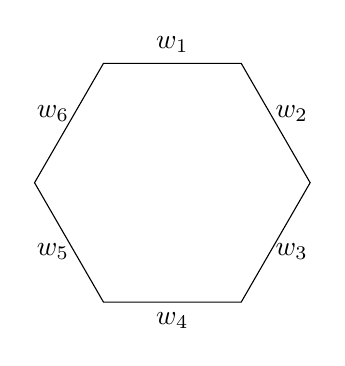
\begin{tikzpicture}
   \newdimen\R
\R=1.75cm
   \draw (0:\R)
   \foreach \x in {60,120,...,360} {  -- (\x:\R) }
 -- cycle (330:\R) node {$w_3$}
 -- cycle (270:\R) node {$w_4$}
 -- cycle (210:\R) node {$w_5$}
 -- cycle (150:\R) node {$w_6$}
 -- cycle  (90:\R) node {$w_1$}
 -- cycle  (30:\R) node {$w_2$};
\end{tikzpicture}
\caption{Sections of city walls}
\label{fig:city-walls}
\end{figure}

Given the scenario described above, as one could expect, the sentence in \ref{ex:explicit-partitives-wall-coll-italian} would be true if two parts of two distinct walls making up the complex were red, e.g., a part of $w_1$ and a part of $w_3$. But surprisingly, unlike \ref{ex:explicit-partitives-wall-pl-italian}, it would also be true if two distinct individual walls making up the complex were red, e.g., the wall $w_1$ and the wall $w_3$, or if two continuous sections of the walls making up the complex were red, e.g., the subsets $\{w_1, w_2\}$ and $\{w_4, w_5\}$. In other words, the meanings that are impossible in explicit set partitives with regular plurals, are easily available with irregular plurals. However, as already mentioned, there is a crucial constraint on possible interpretations of \ref{ex:explicit-partitives-wall-coll-italian}. Namely, one can count parts of the plurality consisting of the walls in question as one as long as they form a contiguous section of the whole structure, i.e., \ref{ex:explicit-partitives-wall-coll-italian} would not be true of two arbitrary pluralities constituted by walls that are not in a tangential relationship with each other. In particular, it would be false if, say, the wall $w_1$ as well as the walls $\{w_3, w_5\}$ were red.\footnote{I assume here the `exact $n$' interpretation of numerals (e.g., \citealt{horn1992said,geurts1998scalars,breheny2005some}; see also \citealt{geurts2006take} for an overview). Notice that the judgments do not change if the numeral is modified by overt \textit{exactly}.}\largerpage[2]

Likewise, assume a slightly morbid scenario involving a decaying human bone or skeleton and consider the contrasts between the examples in \ref{ex:explicit-partitives-bone-italian}.  

\ex.\label{ex:explicit-partitives-bone-italian} Italian (Enrico Flor, p.c.)
\ag. Tre   parti del    osso sono cariate.\label{ex:explicit-partitives-bone-sg-italian}\\
    three parts of.the bone are  decayed\\
    `Three parts of the bone are decayed.'
\bg. Tre parti degli ossi sono cariate.\label{ex:explicit-partitives-bone-pl-italian}\\
    three parts of.the bones are  decayed\\
    `Three parts of the bones are decayed.'
    \a. part-of-a-singularity reading
    \b. \#part-of-a-plurality reading
    \z.
\bg. Tre   parti delle  ossa sono cariate.\label{ex:explicit-partitives-bone-coll-italian}\\
    three parts of.the bones.\textsc{coll} are  decayed\\
    `Three parts of the skeleton are decayed.'
    \a. part-of-a-singularity reading
    \b. part-of-a-plurality reading
    \z.

Given that there is one relevant bone, the entity partitive in \ref{ex:explicit-partitives-bone-sg-italian} gets a part-of-a-singularity reading as usual, and thus the sentence would be true if there were three decayed spots on, e.g., a femur. This is not surprising and, similar to the interpretation of \ref{ex:explicit-partitives-bone-pl-italian}, fits the discussed semantic shift regarding modified explicit set partitives. However, the partitive involving the irregular plural \textit{ossa} in \ref{ex:explicit-partitives-bone-coll-italian} behaves differently. Seemingly, the most readily available interpretation of the example concerns three groups of connected bones making up the skeleton, e.g., it would be true of a decayed femur and knee, a decayed ulna and radius, and the decayed neck and skull. The sentence would be felicitous if three separate bones decayed though, e.g., a femur, ulna, and the skull. Furthermore, analogously to \ref{ex:explicit-partitives-bone-pl-italian} it would be judged true if there were decayed parts on three distinct bones, e.g., a part of the femur, a part of the ulna, and a part of the skull. But again, the reading that \ref{ex:explicit-partitives-bone-coll-italian} cannot get involves three collections of disconnected bones. For instance, it would be infelicitous in a scenario where, say, a femur and the skull, a radius and a knee, and a rib and an ankle bone are decayed. That is because these pairs of bones do not form cohesive wholes, i.e., topologically continuous entities of a particular sort, and consequently cannot be conceptualized as units one could quantify over.

\tabref{tab:properties-of-italian-parte} summarizes the patterns we have observed so far. Specifically, the quantificational behavior of the Italian part-word \textit{parte} depends on certain denotational properties of expressions it combines with. The labels `bare' and `count' in the table stand for bare explicit partitives and count explicit partitives, respectively, each of which can include a singular, a regular plural, or an irregular plural DP.

    \begin{table}[h]
    \centering
\begin{tabular}{lcccccc}
\lsptoprule
                           & \multicolumn{2}{c}{\textsc{singulars}}          & \multicolumn{2}{c}{\textsc{regular pl}}    & \multicolumn{2}{c}{\textsc{irregular pl}}  \\
                           & bare & count & bare & count & bare & count \\ \midrule
subatomic quantification   & $\checked$                   & $\checked$                    & *                              & $\checked$                    & $\checked$                   & $\checked$                    \\
quantification over wholes & *                              & *                               & $\checked$                   & *                               & $\checked$                   & $\checked$                    \\ \lspbottomrule
\end{tabular}
\caption{Properties of Italian \textit{parte} `part' in explicit partitives}
\label{tab:properties-of-italian-parte}
\end{table}

The investigation into the interaction between cardinal numerals and partitives involving Italian irregular plurals leads to a somewhat surprising conclusion. It turns out that the cross-linguistic observation concerning different properties of partitive words in entity and set partitives as discussed in \sectref{sec:partitivity-and-countability} actually does not provide evidence for distinct part-whole structures for singulars and plurals, as suggested by \citet{schwarzschild1996pluralities}. That is not to say that there is no difference in how constitution of objects as opposed to sums thereof is conceptualized. That is to say that the Italian data suggest that the difference does not regard the relation between parts and a whole, but rather that it regards the relation governing how parts are organized in space with respect to each other. In particular, regular plurals encode no topological relations between entities making up pluralities or, in other words, simply denote arbitrary sums of individuals. Consequently, parts of a plurality do not form an integrated entity that could be considered as a unit one could assign a number to, which seems to be a prerequisite for numerical quantification. On the other hand, despite the plurality inference, Italian irregular forms in \textit{-a} differ significantly from regular plurals and somewhat resemble singulars in that they do encode how parts are organized with respect to each other. Specifically, their extensions consist of cohesive aggregates, i.e., pluralities arranged in a particular spatial configurations such that individual objects making up a plurality are either connected or at least stay in a relatively stable proximity. Given that the domain of quantification consists of entities conceptualized as such clusters, counting parts consisting of several singularities is possible as long as they form integrated fragments or continuous sections of the whole. Therefore, I posit that the explanation of the patterns summarized in \tabref{tab:properties-of-partitive-words} and \ref{tab:properties-of-italian-parte} should be contingent on the manner how we conceptualize topological relations holding between parts of different types of entities as well as on the sensitivity of quantificational operations employed in natural language to such relations.

\section{Parts vs. subsets}\label{sec:parts-vs-subsets}

The Italian data provide intriguing evidence but let us hold on for a minute and reconsider the claim that being countable is a property of only those entities that are integrated wholes. One could wonder to what extent the fact that count explicit partitives involving regular plural DPs cannot quantify over sums and can only refer to parts of singular objects tells us anything about the nature of countability. After all, to the extent they are pragmatically admissible, sentences in which the cardinal modifies an expression such as \textit{subset} instead of a part-word are definitely compatible with an interpretation where the domain of quantification consists of collections of individuals, i.e., felicitous when counting subsets of a larger set. For instance, unlike \ref{ex:partitive-numeral-part-polish} the sentence in \ref{ex:partitive-numeral-subset-polish} would be true in a situation where there are, say, ten relevant apples $\{a_1, \dots, a_{10}\}$ and three arbitrary subsets of the apples got spoiled, e.g., $\{a_1, a_2\}$, $\{a_3, a_4, a_5\}$ and $\{a_6, a_7\}$.\footnote{This reading is different from a type of reading discussed in \sectref{sec:mass-parts-quantitifes-and-pieces} where reference to three-fourths of the total volume of the apples would be involved. What is crucial for the discussion of \ref{ex:partitive-numeral-part-polish} is that the quantified subsets of individuals cannot be arbitrary.} In other words, is it really the case that counting requires units that are integrated objects? Or maybe there is simply something weird about partitive words and we should not jump to a conclusion concerning countability based on the partitive data? 

\ex.\label{ex:partitive-numeral-subset-part-polish} Polish
\ag. Trzy podzbiory jabłek zgniły.\label{ex:partitive-numeral-subset-polish}\\
three subsets apples\textsc{.gen} rotted\\
`Three subsets of the apples got spoiled.'
\bg. Trzy części jabłek zgniły.\label{ex:partitive-numeral-part-polish}\\
three parts apples\textsc{.gen} rotted\\
`Three parts of the apples got spoiled.'
\a. part-of-a-singularity reading
\b. \#part-of-a-plurality reading
\z.

At first blush, this seems to be a justified objection and I think it should be taken seriously. However, there are a number of empirical facts suggesting that what happens in \ref{ex:partitive-numeral-subset-polish} is very different from what happens in \ref{ex:partitive-numeral-part-polish}. First of all, it is crucial to emphasize that natural language expressions such as \textit{set} or \textit{subset} are not merely linguistic reflections of set-theoretic concepts involving notions such as $\{\dots\}$ or relations $\subseteq$ and $\subset$. On the contrary, such expressions have a number of properties that classify them on a par with group nouns such as \textit{committee}, \textit{band}, or \textit{pile}.\footnote{In the following text, I will ignore the evidence for distinguishing between different classes of group nouns \citep[see][]{pearson2011new,henderson2017swarms,docekal_wagiel2018decomposing} and assume that for our purposes there are no relevant differences between nouns such as \textit{band} and \textit{pile}.} On the other hand, similarly to bare plurals set partitives refer to pluralities but part-words are not collectives, as attested by a number of tests involving predicate non-sharing. 

It has been proposed in the literature that group nouns and plural NPs do not co-refer since one can find multiple contrasts concerning (in)compatibility with certain predicates \citep{barker1992group,schwarzschild1996pluralities}. For instance, the sentence with a collective DP as a subject is perfectly fine with the predicate \textit{have five members}, see \ref{ex:collectives-members}, but its altered version involving a plural DP as in \ref{ex:plurals-members} is not.

\ex.\label{ex:collectives-plurals-members} English \citep[p. 153]{lonning1987mass}
\a. The committee has five members.\label{ex:collectives-members}
\b. \#The men have five members.\label{ex:plurals-members}

Now, let us test the behavior of the Polish part-word \textit{część} `part' with respect to plurals, regular collective nouns, and the expression \textit{podzbiór} `subset'.\footnote{It needs to be admitted that due to the restricted distribution of the noun \textit{podzbiór} (often limited to mathematical and computational contexts) the following sentences involving this expression is not how people usually talk. Rather, these examples sound nerdy or somewhat like clumsily worded math exercises rather than something a regular person would say. Nevertheless, despite the slight lexical oddity the judgments concerning compatibility with different predicates, interactions in co-variational contexts and with overt distributive operators seem to be rather clear.} The contrasts in \ref{ex:plurals-part-collectives-subset-polish-elements} show that bare plurals and bare explicit set partitives differ from the typical group noun \textit{stos} `pile' as well as \textit{podzbiór} in that they are not compatible with predicates of the type \textit{have ten elements}, which are assumed to indicate bunches \citep{schwarzschild1996pluralities}. 

\ex.\label{ex:plurals-part-collectives-subset-polish-elements} Polish
\ag. \#Jabłka składają się z dziesięciu sztuk.\label{ex:plurals-polish-elements}\\
apples consist \textsc{refl} from ten\textsc{.gen} items\textsc{.gen}\\
Intended: `The apples consist of ten items.'
\bg. \#Część jabłek składa się z dziesięciu sztuk.\label{ex:part-polish-elements}\\
part apples\textsc{.gen} consist \textsc{refl} from ten\textsc{.gen} items\textsc{.gen}\\
Intended: `Some of the apples consist of ten items.'
\bg. Stos jabłek składa się z dziesięciu sztuk.\label{ex:collectives-polish-elements}\\
pile apples\textsc{.gen} consist \textsc{refl} from ten\textsc{.gen} elements\textsc{.gen}\\
`The pile of apples consists of ten items.'
\bg. Podzbiór jabłek składa się z dziesięciu sztuk.\label{ex:subset-polish-elements}\\
subset apples\textsc{.gen} consist \textsc{refl} from ten\textsc{.gen} elements\textsc{.gen}\\
`The subset of apples consists of ten items.'

The same pattern can be observed when the examined expressions appear as first arguments of the two-place predicate \textit{należy do} `belongs to' which arguably designates assignment of objects to some abstract entity representing a collection. Though both \ref{ex:collectives-polish-belong} and \ref{ex:subset-polish-belong} are felicitous, the sentences including plurals and explicit set partitives in \ref{ex:plurals-polish-belong} and \ref{ex:part-polish-belong}, respectively, cannot saturate the predicate.

\ex.\label{ex:plurals-part-collectives-subset-polish-belong} Polish
\ag. \#Ta papierówka należy do jabłek.\label{ex:plurals-polish-belong}\\
this white.transparent belongs to apples\textsc{.gen}\\
Intended: `This white transparent apple belongs to the apples.'
\bg. \#Ta papierówka należy do części jabłek.\label{ex:part-polish-belong}\\
this white.transparent belongs to part\textsc{.gen} apples\textsc{.gen}\\
Intended: `This white transparent apple belongs to some of the apples.'
\bg. Ta papierówka należy do stosu jabłek.\label{ex:collectives-polish-belong}\\
this white.transparent belongs to pile\textsc{.gen} apples\textsc{.gen}\\
`This white transparent apple belongs to the pile of apples.'
\bg. Ta papierówka należy do podzbioru jabłek.\label{ex:subset-polish-belong}\\
this white.transparent belongs to subset\textsc{.gen} apples\textsc{.gen}\\
`This white transparent apple belongs to the subset of apples.'

Another contrast between plurals and collective nouns concerns distribution with reciprocals, as demonstrated in \ref{ex:reciprocals}. 

\ex.\label{ex:reciprocals} English \citep[p. 168]{schwarzschild1996pluralities}
\a. The rocks in that pile are touching each other.\label{ex:reciprocals-plural}
\b. \# That pile is touching each other.\label{ex:reciprocals-group}

Polish examples such as those in \ref{ex:plurals-part-collectives-subset-polish-reciprocals} show that there is a contrast between bare plurals and bare explicit set partitives, on the one hand, and typical collectives such as \textit{stos} and \textit{podzbiór}, on the other. 

\ex.\label{ex:plurals-part-collectives-subset-polish-reciprocals} Polish
\ag. Jabłka dotykają się nawzajem.\label{ex:plurals-polish-reciprocals}\\
apples touch \textsc{refl} each-other\\
`The apples are touching each other.'
\bg. Część jabłek dotyka się nawzajem.\label{ex:part-polish-reciprocals}\\
part apples\textsc{.gen} touches \textsc{refl} each-other\\
`Some of the apples are touching each other.'
\bg. \#Stos jabłek dotyka się nawzajem.\label{ex:collectives-polish-reciprocals}\\
pile apples\textsc{.gen} touches \textsc{refl} each-other\\
Intended: `The pile of apples touches each other.'
\bg. \#Podzbiór jabłek dotyka się nawzajem.\label{ex:subset-polish-reciprocals}\\
subset apples\textsc{.gen} touches \textsc{refl} each-other\\
Intended: `The subset of the apples touches each other.'

Plurals and explicit set partitives combine felicitously with reciprocal expressions, whereas collectives do not. In particular, \ref{ex:plurals-polish-reciprocals} and \ref{ex:part-polish-reciprocals} indicate either strong or intermediate reciprocity \citep{fiengo_lasnik1973logical,dalrymple1998reciprocal,beck2001reciprocals}, i.e., either each of the apples in question is touching all the other apples or any  two of the apples are connected by a chain of apples that  stand in the reciprocal relation. Nevertheless, it is impossible to define such truth conditions for \ref{ex:collectives-polish-reciprocals} and \ref{ex:subset-polish-reciprocals}.

A similar distribution is attested in contexts where the reciprocal is covert, see \ref{ex:covert-reciprocal}, including co-variational environments such as \ref{ex:covariation}. Specifically, plurals do combine with predicates triggering covariation, whereas group nouns do not. 

\ex.\label{ex:covert-reciprocal} English \citep{dougherty1970grammar}
\b.[] \# The trio collided. 

\ex.\label{ex:covariation} English \citep[p. 168]{schwarzschild1996pluralities}
\a. The members of group A live in different cities.\label{ex:covariation-plural}
\b. \# Group A lives in different cities.\label{ex:covariation-group}

Let us then consider Polish examples involving plurals, explicit partitives, group nouns, and phrases headed by \textit{podzbiór} in subject position, as provided in \ref{ex:covariation-polish} and \ref{ex:distributivity-polish}. In \ref{ex:covariation-polish-plural}, the sentence-internal \textit{different} expression \textit{w różnych miastach} `in different cities' is bound within a clause to express covariation with a plural argument due to a built-in distributive operator \citep{carlson1987same,beck2000semantics,brasoveanu2008sentence,dotlacil2010anaphora}. As a result, the sentence would be true if for each of the musicians it were the case that they lived in a city that is different from the cities other musicians live in. Due to this kind of meaning, sentence-internal \textit{different} expressions are good indicators of distributivity.\largerpage

    \ex. Polish\label{ex:covariation-polish} 
    \ag. Muzycy mieszkają w różnych miastach.\label{ex:covariation-polish-plural}\\
	musicians live in different\textsc{.loc} cities\textsc{.loc}\\
	`The musicians live in different cities.'
	\bg. Część muzyków mieszka w różnych miastach.\label{ex:covariation-polish-part}\\
	part musicians\textsc{.gen} lives in different\textsc{.loc} cities\textsc{.loc}\\
	`Some of the musicians live in different cities.'
	\bg. \# Zespół mieszka w różnych miastach.\label{ex:covariation-polish-group}\\
	band live in different\textsc{.loc} cities\textsc{.loc}\\
	Intended: `The band lives in different cities.'
    \bg. \# Podzbiór muzyków mieszka w różnych miastach.\label{ex:covariation-polish-subset}\\
	subset musicians\textsc{.gen} lives in different\textsc{.loc} cities\textsc{.loc}\\
	Intended: `A subset of the musicians lives in different cities.'

The sentences in \ref{ex:distributivity-polish} include the distributive preposition \textit{po} which is a marker for distant distributivity in Polish \citep[e.g.,][]{przepiorkowski2008generalised,przepiorkowski2010towards,przepiorkowski2014distance,przepiorkowski-patejuk2013syntax}.\footnote{For detailed studies on distant distributivity and distributive \textit{po} in Slavic see also, e.g., \citet{franks1994parametric,franks1995parameters}, \citet{harves2003getting}, and \citet{knezevic2015numerals}.} As such, similarly to binominal \textit{each} \citep[e.g.,][]{safir_stowell1988binominal,zimmermann2002boys,dotlacil2012binominal,champollion2012each} and distributive numerals \citep[e.g.,][]{gil2002distributive,oh2005plurality,cable2014distributive,hofherr_etxeberria2017distributive} \textit{po} marks the distributive share and distributes it over the distributive key denoted by a different phrase, here the subject DP. As a result, the possibility of a collective reading is ruled out and a sentence in which \textit{po} occurs is obligatorily interpreted distributively, e.g., in \ref{ex:distributivity-polish-plural} each of the musicians played a song. This conflicts with the semantics of group nouns which in general do not allow for the access to individual members of a collection, hence \ref{ex:distributivity-polish-group} is an awkward sentence. As witnessed by the contrast between \ref{ex:distributivity-polish-part} and \ref{ex:distributivity-polish-subset}, explicit set partitives pattern with plurals, whereas \textit{podzbiór} behaves as typical collectives.

	\ex. Polish\label{ex:distributivity-polish}
    \ag. Muzycy zagrali po piosence.\label{ex:distributivity-polish-plural}\\
	musicians played \textsc{distr} song\textsc{.loc}\\
	`The musicians played a song each.'
	\bg. Część muzyków zagrała po piosence.\label{ex:distributivity-polish-part}\\
	part musicians\textsc{.gen} played \textsc{distr} song\textsc{.loc}\\
	`Some of the musicians played a song each.'
	\bg. \# Zespół zagrał po piosence.\label{ex:distributivity-polish-group}\\
	band played \textsc{distr} song\textsc{.loc}\\
	Intended: `The band played a song each.'
    \bg. \# Podzbiór muzyków zagrał po piosence.\label{ex:distributivity-polish-subset}\\
	subset musicians\textsc{.gen} played \textsc{distr} song\textsc{.loc}\\
	Intended: `A subset of the musicians played a song each.'
    
Yet another diagnostic involves the VP disjunction test proposed by \citet[pp. 30--31]{de_vries2015shifting}. When the test is applied, \textit{część} does not exhibit the kind of behavior associated with group nouns. To illustrate this, let us consider the sentences in \ref{ex:vp-disjunction-plural}.

\ex. English \citep[p. 31; adapted]{de_vries2015shifting}
\a. The children are singing or dancing.\label{ex:vp-disjunction-plural}
\a. collective reading\label{ex:vp-disjunction-plural-coll}
\b. distributive reading\label{ex:vp-disjunction-plural-distr}
\z.
\b. The team is singing or dancing.\label{ex:vp-disjunction-group}
\a. collective reading\label{ex:vp-disjunction-group-coll}
\b. \#distributive reading\label{ex:vp-disjunction-group-distr}
\z.

In \ref{ex:vp-disjunction-plural}, the definite plural DP \textit{the children} serves as a subject of the disjunctive sentence. There are two possible interpretations of \ref{ex:vp-disjunction-plural}. On the collective interpretation, see \ref{ex:vp-disjunction-plural-coll}, the disjunction \textit{singing or dancing} holds of the plurality as a whole. In other words, it is either the case that all the relevant children are singing or that all the relevant children are dancing. However, there is yet another reading of \ref{ex:vp-disjunction-plural}, namely the distributive interpretation, see \ref{ex:vp-disjunction-plural-distr}, according to which the disjoined VPs hold not of the plurality of children as a whole but rather of each individual child. Thus, some of the children might be singing while others might be dancing. Crucially, when the definite plural is replaced with a group noun such as \textit{team} as in \ref{ex:vp-disjunction-group}, the distributive interpretation is no longer available. The only reading such a sentence can get is that the whole plurality was either involved in singing or in dancing.

Now, let us examine the behavior of Polish nouns \textit{część} and \textit{podzbiór} compared to plurals and group nominals in sentences involving VP disjunction such as those in \ref{ex:vp-disjunction-polish}. 
	
	\ex.\label{ex:vp-disjunction-polish} Polish
    \ag. Dzieci tańczą lub śpiewają.\label{ex:vp-disjunction-polish-plural}\\
	children dance or sing\\
	`The children are dancing or singing.'
	\a. collective reading
	\b. distributive reading
	\z.
	\bg. Grupa dzieci tańczy lub śpiewa.\label{ex:vp-disjunction-polish-group}\\
	group children\textsc{.gen} dances or sings\\
	`The group of children is dancing or singing.'
	\a. collective reading
	\b. \#distributive reading
	\z.
	\bg. Część dzieci tańczy lub śpiewa.\label{ex:vp-disjunction-polish-part}\\
	part children\textsc{.gen} dances or sings\\
	`Some children are dancing or singing.'
	\a. collective reading
	\b. distributive reading
    \z.
   \pagebreak\bg. Pozbiór dzieci tańczy lub śpiewa.\label{ex:vp-disjunction-polish-subset}\\
   subset children\textsc{.gen} dances or sings\\
   `A subset of children is dancing or dancing.'
   	\a. collective reading
	\b. \#distributive reading
    \z.

The example \ref{ex:vp-disjunction-polish-plural} can have either a collective or a distributive reading, i.e., it would be true either when all the children are dancing or singing or when some are dancing whereas others are singing. On the other hand, a sentence with a group noun as a subject like \ref{ex:vp-disjunction-polish-group} can only be interpreted collectively. That is also the case in \ref{ex:vp-disjunction-polish-subset}, i.e., all the children in the relevant subset need to be either dancing or singing. However, \ref{ex:vp-disjunction-polish-part} is felicitous in both collective and distributive scenarios. Once again, the \textit{part} word \textit{część} patterns with plurals rather than collectives, which definitely proves that it differs from expressions such as \textit{subset}.

Notice that whatever theory of the relationship between agreement and collectivity/distributivity one might have (e.g., \citealt{de_vries2015shifting}; see also \citealt{schwarzschild1996pluralities} and \citealt{pearson2011new} for the discussion of group nouns in British English as well as  \citealt{bosnic2016distributivity} for experimental data concerning distributivity and agreement mismatches in BCS), it cannot explain the semantic difference between \textit{part} expressions and group nouns. In Polish, \textit{część} just like \textit{zespół} (and any other group noun) triggers singular agreement on the verb. As witnessed by the glosses in the examples provided above, in sentences with both explicit partitives and group nouns, see \ref{ex:covariation-polish-part}--\ref{ex:covariation-polish-group} and \ref{ex:vp-disjunction-polish-group}--\ref{ex:vp-disjunction-polish-part}, the verbs agree in number with the subjects. Furthermore, both in \ref{ex:distributivity-polish-part} and \ref{ex:distributivity-polish-group} the past participles agree with \textit{część} and \textit{zespół} in gender by taking the feminine and masculine form, respectively. Therefore, it is not the agreement pattern but rather lexical properties of \textit{część} that are accountable for the semantic difference.

Finally, despite being distinct syntactic categories partitive words pattern with cardinal numerals in that in general they allow for modification by class A/B modifiers such as \textit{more than} and \textit{at least} \citep{nouwen2010two,nouwen2016plurality,brasoveanu2012modified}, see \ref{ex:partitives-polish-modifiers}.\footnote{Since there are some restrictions in this respect which I believe result from the indefinite nature of some partitive words, I present here only parallel examples with class B modifiers.} This again suggests that their semantics includes a purely quantificational component.

\ex.\label{ex:partitives-polish-modifiers} Polish
\ag. {Co najmniej} część murów jest czerwona.\label{ex:explicit-partitives-polish-at-least} \\
at.least part walls\textsc{.gen} is red\\
`At least some of the walls are red.'
\bg. {Co najwyżej} część murów jest czerwona.\label{ex:explicit-partitives-polish-at-most} \\
at.most part walls\textsc{.gen} is red\\
`At most some of the walls are red.'
\bg. {Co najmniej} połowa murów jest czerwona.\label{ex:proportional-partitives-polish-at-least} \\
at.least half walls\textsc{.gen} is red\\
`At least half of the walls are red.'
\bg. {Co najwyżej} połowa murów jest czerwona.\label{ex:proportional-partitives-polish-at-most} \\
at.most half walls\textsc{.gen} is red\\
`At most half of the walls are red.'
\bg. {Co najmniej} pięć murów jest czerwonych.\label{ex:count-partitives-polish-at-least} \\
at.least five walls\textsc{.gen} is red\\
`At least five of the walls are red.'
\bg. {Co najwyżej} pięć murów jest czerwonych.\label{ex:count-partitives-polish-at-most} \\
at.most five walls\textsc{.gen} is red\\
`At most five of the walls are red.'

The results of a battery of tests applied to the Polish nouns \textit{część} `part' and \textit{podzbiór} `subset' unequivocally indicate that \textit{podzbiór} is a group noun,\footnote{\citeauthor{schwarzschild1996pluralities} (\citeyear[p. 168]{schwarzschild1996pluralities}) actually lists \textit{set} among group nouns.} and thus triggers obligatory collective interpretations of sentences in which it occurs, whereas \textit{część} patterns with plurals including being ambiguous between collective and distributive readings. This is a significant contrast between the expressions in question suggesting that their extensions differ in a significant way. In particular, it has been commonly advocated in the literature that group nouns do not refer to pluralities but rather to atomic individuals, i.e., somewhat abstract singularities that might be associated with their members \citep[e.g.,][]{barker1992group,schwarzschild1996pluralities,winter2001flexibility,champollion2017parts}.\footnote{But see, e.g., \citet{link1984hydras,link1998algebraic}, \citet{landman1989groupsi,landman1989groupsii,landman2000events}, and \citet{de_vries2015shifting} for an alternative view on which a group noun denotes a special type of plurality shifted to an impure atom or group-atom depending on a particular approach. \citet{pearson2011new}, on the other hand, proposes that group nouns are predicates of individual concepts.} Whatever extraordinary properties such atoms have, it is plausible to assume that they are conceptualized as something distinct from mere sums of objects.

Therefore, I conclude that explicit partitives refer to genuine pluralities where\-as group nouns including expressions such as \textit{set} and \textit{subset} denote abstract entities that are associated with pluralities of their members but are ontologically distinct from them. Having this in mind, there is nothing surprising about the fact that count explicit set partitives do not quantify over sums of individuals, and in fact, it turns out that part-words actually pattern with regular nominals, as will be shown below. 

It has been observed for a long time that the semantics of numeral phrases in languages such as English poses a compositional puzzle. On the one hand, cardinal numerals higher than \textit{one} combine only with plural nominals, on the other, plural NPs modified by cardinals are interpreted as singular expressions. Specifically, although plurals denote sums of entities, the domain of quantification is always a set of atomic individuals (\citealt{kratzer1989investigation}; \citealt{chierchia1998reference}; \citealt{landman2000events}; see also \citealt{kobuchi-philip2006identity}). Contrary to what one would expect if numerals simply counted elements in a given set \citep[e.g.,][]{barwise_cooper1981generalized} and combined with plural nouns in a straightforward manner, cardinals seem to be sensitive only to singular individuals in the sense that they do not assign numbers to sums of objects. Actually, this fact has already been realized in the system of \citet{link1983logical} where the extension of a phrase such as \textit{three children} is supposed to contain only special types of elements, namely exactly three atoms. To illustrate why such a restriction is necessary, let us consider the sentence in \ref{ex:domain-of-quantification-example}.   

\ex.\label{ex:domain-of-quantification} \a. Three children slept.\label{ex:domain-of-quantification-example}		
	 \b. $\llbracket \text{children} \rrbracket = \{a, b, c, d, ab, ac, ad, bc, bd, cd, abc, abd, acd, bcd, abcd\}$\label{ex:domain-of-quantification-numeral-phrase}
     \b. $\llbracket \text{three children} \rrbracket \cap \llbracket \text{slept} \rrbracket = \{a, ab, abcd\}$\label{ex:domain-of-quantification-wrong-meaning1}
     \b. $\llbracket \text{three children} \rrbracket \cap \llbracket \text{slept} \rrbracket = \{a, b, ab\}$\label{ex:domain-of-quantification-wrong-meaning2}

Let us assume that there are four relevant children in the universe of discourse, say, Anne, Betty, Carl, and Danny, i.e., $a$, $b$, $c$, and $d$ respectively. Then the meaning of the plural noun \textit{children} is the set involving both atomic children and all the sums generated by joining the atoms, see \ref{ex:domain-of-quantification-numeral-phrase}. If \textit{three} simply counted the elements in the set denoted by the modified noun, among the possible verifications of the sentence in \ref{ex:domain-of-quantification-example} would be \ref{ex:domain-of-quantification-wrong-meaning1} and \ref{ex:domain-of-quantification-wrong-meaning2} since in both cases the set of children that slept consists of three elements.

The truth conditions in \ref{ex:domain-of-quantification-wrong-meaning1} and \ref{ex:domain-of-quantification-wrong-meaning2} predict \ref{ex:domain-of-quantification-example} to be true both in a scenario where there were four individual children sleeping and in a scenario where only two individual children slept. However, this not how the sentence is understood. It seems that what cardinals in a language such as English do is that they restrict possible verifications of sentences including numeral phrases in such a way that sums of individuals are excluded from the domain of quantification.\footnote{Alternatively, one might assume that there is a null classifier responsible for this restriction \citep[e.g.,][]{selkirk1977some,kobuchi-philip2006identity}.} 

With this in mind, let us return to count explicit partitives such as the Italian examples in \ref{ex:count-explicit-partitives-italian}, repeated here as \ref{ex:count-explicit-partitives-italian2}. Similarly to regular plural DPs, unmodified explicit set partitives denote pluralities or, more precisely, sub-pluralities. However, when combined with a numeral they do not allow for quantification over sub-pluralities but only over material parts of individuals making up pluralities.  

\ex.\label{ex:count-explicit-partitives-italian2} Italian \citep[p. 186; adapted]{schwarzschild1996pluralities}
\ag. tre parti del muro\label{ex:count-explicit-entity-partitives-italian2}\\
three parts of.the wall\\
`three parts of the wall'
\bg. tre parti dei muri\label{ex:count-explicit-set-partitives-italian2}\\
three parts of.the walls\\
`three parts of the walls'
\a. part-of-a-singularity reading
\b. \#part-of-a-plurality reading
\z.

At first blush, it seems surprising but actually in languages such as English the same effect can be found in numeral phrases. Specifically, the numeral combines with the plural noun which denotes a set of pluralities; however, the domain of quantification does not consist of pluralities but rather atomic individuals. Hence, as demonstrated in \ref{ex:count-explicit-partitives-numeral-phrases} the phrase \textit{three walls} does not mean three pluralities of walls but rather a plurality of three walls. Likewise, the Italian partitive phrase in \ref{ex:count-explicit-set-partitives-italian2} cannot be interpreted as three pluralities of sub-pluralities of walls. Instead, it would be felicitously paraphrased as a plurality of three parts of walls.

		\ex. Pluralities of wholes and parts\label{ex:count-explicit-partitives-numeral-phrases}
        \a. three walls
		\a. \#three pluralities of walls
		\b. plurality of three walls
        \z.
        \b. tre parti dei muri
		\a. \#three pluralities of parts-of-a-plurality of walls
		\b. plurality of three parts of walls
		\z.
		
In this section, I argued that set partitives differ from collectives and discussed a number of issues regarding the domain of quantification in count explicit partitives as well as group nouns and plurals modified by cardinal numerals. An important question that arises after examining the evidence explored in this chapter is why natural language does not allow for counting a sum of entities as one thing unless it satisfies certain topological (or other) criteria. 

\section{Summary}\label{sec:summary-ch2}

The data discussed in this chapter provide compelling evidence that cross-linguis\-tically it is common for the same partitive word including proportional quantifiers such as half-words to appear both in entity and set partitives. This fact suggests that such expressions can operate both at the superatomic and subatomic level depending on what structure is provided by the embedded DP. Furthermore, on the basis of the zeugma test involving German partitives with conjoined singular and plural DPs I showed that it is empirically inadequate to account for the parallelism between explicit and proportional entity and set partitives in terms of semantic ambiguity. 

However, at the same time explicit partitives modified by a cardinal numeral can only quantify over material parts of singular individuals irrespective of \linebreak whether the complement DP is singular or plural. At first sight, this fact seems to be at variance with the claim that there is unified parthood utilized by partitive words in both entity and set partitives. Nonetheless, an important empirical finding concerning Italian irregular plurals showed that if a plural expression encodes a certain topological configuration, i.e., denotes entities conceptualized as cohesive pluralities, count explicit partitives can get a part-of-a-plurality reading in such a case. This fact demonstrates that the uncountability of explicit partitives with plurals does not indicate per se different part-whole structures for singularities and pluralities. Rather, countability results from the interplay between the meaning of a partitive word and the extension of a singular or plural DP it combines with, and topological constraints play a crucial role in this interaction.

Given the cross-linguistic and intra-linguistic evidence explored in this chapter, the two remaining possibilities are the following. It is either the case that singulars and plurals employ a unified part-whole structure or that their mereologies do differ but at the same time partitive words involve a derived indeterminate notion of parthood which allows them to quantify over elements of whatever part-whole structure they are applied to. I argue for the first option. However, by advocating this claim I do not advance a view that singulars and plurals employ the same structures. What I claim is that it is not the part-whole relation that differs but rather that there is another notion involved which is responsible for how parts are topologically arranged with respect to each other. Intuitively, this seems correct since we conceptually distinguish between integrated wholes and arbitrary sums of parts, and quantification in natural language is sensitive to the distinction. Specifically, only things conceptualized as integrated parts of integrated wholes can be assigned numbers when counting. On the other hand, scattered entities such as pluralities are prohibited from the domain of quantification cardinal numerals establish unless certain individuation criteria are satisfied. In addition, Italian irregular plurals provide evidence that there are natural language expressions involving yet another type of structure. In particular, such nominals designate entities that are similar to plurals in that they consist of multiple integrated objects, but at the same time the sum thereof is arranged in a particular way, i.e., it constitutes a cluster.

So far, I have argued that explicit and proportional partitives provide evidence that countability is restricted to entities that form an integrated whole as typically denoted by concrete singular count nouns, while the arbitrary sums of parts regular plural nouns refer to cannot be counted. Furthermore, the data concerning subatomic quantification suggests that this constraint is also applicable at the level of material parts of individuals. If that is correct, one would expect that there are natural language expressions dedicated exclusively to quantification over integrated parts similar to cardinal numerals that count integrated wholes. In the next section, I will introduce novel data concerning distinct types of half-words in Polish as well as other partitive expressions.

\chapter{Exploring topological sensitivity}\label{ch:exploring-topological-sensitivity}

In the previous chapter, I discussed data concerning quantification over parts in explicit entity and set partitives. Specifically, I presented  evidence suggesting that only integrated parts of integrated wholes can be subject to counting. As I have already indicated in the introduction, in English the difference can be captured by the contrast between bare \textit{part} and \textit{a part}. I argued that expressions corresponding to the former refer to arbitrary parts of a whole including discontinuous portions of a substance making up a whole, and thus are uncountable. On the other hand, expressions corresponding to the latter refer to continuous integrated parts of a whole and as such can pluralize and combine with cardinals. In this chapter, I explore to what extent natural language is sensitive to this distinction. To this end, I will provide novel evidence from different types of Polish partitive words that encode the contrast formally. It will turn out that this phenomenon is not something idiosyncratic, but rather cross-linguistic evidence suggests that it is relatively widespread with different languages using different means to express it. Moreover, based on the data concerning whole-adjectives I will demonstrate the linguistic relevance of two aspects of being whole, namely maximality and integrity.\footnote{The scope of this chapter would be much narrower if it were not for my informants with whom I tested the interpretation of expressions in languages other than Polish. In particular, I am very grateful to Jonathan Bobaljik, Jeffrey Parrott, and Guy Tabachnick for their judgments and discussion concerning English, to Berit Gehrke, Nina Haslinger, and Maximilian Prüller for German, Erlinde Meertens and Izabela Jordanoska for Dutch, Muriel Assmann for Brazilian Portuguese, and Chang Liu for Mandarin. I would also like to thank Adam Przepiórkowski for sharing his observations regarding Polish with me.}

\section{Continuous and discontinuous parts}\label{sec:continuous-discontinuous-parts}

Given the meaning of the plural in languages such as English, it follows that expressions such as \textit{a part} are incompatible with predicates denoting pluralities. Intuitively, the reason is that the extension of a phrase headed by \textit{a part} comprises integrated portions, i.e., parts that come in one piece, whereas plurals denote arbitrary sums, i.e., scattered entities consisting of discontinuous elements. However, if the plural were augmented with an additional semantic feature guaranteeing that a plurality of integrated objects is itself an integrated object, as is arguably the case in at least some Italian irregular plurals, then an expression corresponding to English \textit{a part} is able to combine with such a plural expression. In such a case, it would yield a part of a plurality whose constituents are in a particular topological relation, namely they are connected to each other.

But is there any additional reason to assume that natural language expressions are sensitive to topological relations operating alongside part-whole structures? And if so, to what extent do the discussed phenomena really tell us something important about countability? The claim advanced here is that what counts as one needs to be an integrated part (proper or improper) of an integrated whole. Though this might seem intuitively correct, a question arises where the property of `coming in one piece' comes from. After all, countability is the ability of an expression to appear in morpho-syntactic environments related to counting, but counting is a semantic operation of assigning numbers to units of a particular type. Hence, one could wonder whether there is evidence that there is something in an expression's meaning that corresponds to the notion of being an integrated entity, and thus being countable. One prominent view holds that countability is not a property of a particular class of nouns but rather of full DPs (e.g., \citealt{borer2005name}, see also \citealt{allan1980nouns} and \citealt{pelletier_schubert1989mass} and the following work by \citeauthor{pelletier2011descriptive}), and thus arises within a complex nominal syntactic structure. On the other hand, other approaches posit that it is lexical meaning that determines countability patterns  \citep[e.g.,][]{wierzbicka1988semantics,wisniewski_lamb_middleteon2003conceptual}. However, the evidence discussed in the literature is mainly restricted to cases of quantification over wholes and almost totally ignores constructions in which what is counted are bits of objects rather than whole individuals.

In this section, I will provide additional evidence for the significance of the role of spatial integrity, i.e., compactness, of parts in subatomic quantification. The core data come from the distribution and semantic properties of distinct classes of Polish half-words.

\subsection{Polish half-words}\label{sec:polish-half-words}

Polish distinguishes lexically between three distinct half-words, as presented in \ref{ex:polish-half-words-morphology}. They are morphologically derived from one another with \textit{pół} being morphologically the least marked form with no derivational affixes. As presented in \ref{ex:polish-half-pol-morphology}, \textit{pół} consists only of a root and null inflectional marker. On the other hand, \textit{połowa} and \textit{połówka} are derived forms involving in addition the morpheme \textit{-ow-/-ów-} as well as the diminutive suffix \textit{-k-} in the latter case, see \ref{ex:polish-half-polowa-morphology}--\ref{ex:polish-half-polowka-morphology}.

		\ex. Polish\label{ex:polish-half-words-morphology}
        \ag. pół-$\varnothing$\\
		root-inflectional.marker\\
		`half$_1$'\label{ex:polish-half-pol-morphology}
		\bg. poł-ow-a\\
		root-derivational.suffix-inflectional.marker\\
		`half$_2$'\label{ex:polish-half-polowa-morphology}
        \bg. poł-ów-k-a\\
		root-deriv.suffix$_1$-deriv.suffix$_2$-infl.marker\\
		`half$_3$'\label{ex:polish-half-polowka-morphology}

In terms of $\phi$-features, \textit{pół} shows neuter agreement whereas \textit{połowa} and \textit{połówka} are feminine, as demonstrated in \ref{ex:polish-half-words-agreement}. Furthermore, similarly to vague quantifiers such as \textit{dużo} `many/much', \textit{pół} is defective in that it has only the nominative/accusative form (though it can also appear in some genitive positions).\footnote{\label{fn:plural-pol}Based on examples from the National Corpus of Polish (NCP) like \ref{ex:inherent-plural}, \citet{przepiorkowski2006inherentnej} argues that \textit{pół} `half' is inherently plural because it can be modified by the plural demonstrative \textit{te} `these'. Notice, however, that though there are definitely varieties of Polish in which \ref{ex:inherent-plural} is well-formed, there are also many speakers (including myself) for whom it is ungrammatical. Furthermore, in modern Polish the neuter singular demonstrative \textit{to} `this' is being gradually replaced by the colloquial form \textit{te} `this' which is homophonous to the plural \textit{te} `these'. It is possible that the acceptability of \ref{ex:inherent-plural} is correlated with this process.

\ex. Polish (NCP)
\bg.[] \%Zaczną się niebawem prace polowe, więc te pół kilometra jest konieczne.\\
will.begin \textsc{refl} soon works field.\textsc{adj} so these half kilometer.\textsc{gen} is necessary\\
`Field work will start soon, so it is necessary (to finish) this half kilometer (road).'\label{ex:inherent-plural}

}\largerpage[2]

\ex. Polish\label{ex:polish-half-words-agreement}
\ag. To czerwone pół jabłka zgniło.\\
this\textsc{.nom.n} red\textsc{.nom.sg.n} half$_{1}$\textsc{.nom.n} apple\textsc{.gen.n} rotted\textsc{.sg.n}\\
`This red half of the apple got spoiled.'
\bg. Ta czerwona połowa jabłka zgniła.\\
this\textsc{.nom.f} red\textsc{.nom.sg.f} half$_{2}$\textsc{.nom.f} apple\textsc{.gen.n} rotted\textsc{.sg.f}\\
`This red half of the apple got spoiled.'
\bg. Ta czerwona połówka jabłka zgniła.\\
this\textsc{.nom.f} red\textsc{.nom.sg.f} half$_{3}$\textsc{.nom.f} apple\textsc{.gen.n} rotted\textsc{.sg.f}\\
`This red half of the apple got spoiled.'

At first blush, the Polish half-words in \ref{ex:polish-half-words-agreement} are mere synonyms making the same contribution to the interpretation of the discussed sentences. However, closer investigation reveals intriguing differences in their distribution and meaning. Let us first consider the most frequent and semantically least marked \textit{half} expression, i.e., \textit{połowa}. As witnessed in \ref{ex:distribution-polowa}, there are no constraints on its distribution and it can felicitously combine with all types of entity-denoting predicates including count singulars, collectives, plurals, and mass terms.\footnote{In this section, I provide the examples with collective nouns only for the sake of completeness, i.e., in order to show the distributional difference between \textit{pół} and \textit{połówka}. In the remaining part of this chapter (except of \sectref{sec:quarter-words}), I will not investigate the interaction between partitives and collectives.}
		
		\ex. Polish\label{ex:distribution-polowa}
        \ag. połowa jabłka\\
		half$_2$ apple\textsc{.gen}\\
		`half of the apple'\label{ex:distribution-polowa-sg}
		\bg. połowa  stosu (jabłek)\\
		half$_2$ pile\textsc{.gen} (apples\textsc{.gen})\\
		`half of the pile (of apples)'\label{ex:distribution-polowa-group}
		\bg. połowa jabłek\\
		half$_2$ apples\textsc{.gen}\\
		`half of the apples'\label{ex:distribution-polowa-pl}
		\bg. połowa soku\\
		half$_2$ juice\textsc{.gen}\\
		`half of the juice'\label{ex:distribution-polowa-mass}

On the other hand, \textit{pół} has a more restricted distribution since it is incompatible with cumulative predicates such as plurals and mass nouns, see \ref{ex:distribution-pol}. Thus, it can only combine with regular count singulars and collective nouns.\largerpage
		
		\ex. Polish\label{ex:distribution-pol}
        \ag. pół jabłka\\
		half$_1$ apple\textsc{.gen}\\
		`half of the apple'\label{ex:distribution-pol-sg}
		\bg. pół stosu \minsp{(} jabłek)\\
		half$_1$ pile\textsc{.gen} {} apples\textsc{.gen}\\
		`half of the pile (of apples)'\label{ex:distribution-pol-group}
		\bg. \# pół jabłek\\
		half$_1$ apples\textsc{.gen}\label{ex:distribution-pol-pl}\\
		Intended: `half of the apples'
		\bg. \# pół soku\\
		half$_1$ juice\textsc{.gen}\label{ex:distribution-pol-mass}\\
		Intended: `half of the juice'

Notice that the constraint on the distribution of \textit{pół} is not morpho-syntactic. The phrases in \ref{ex:pl.tantum-pol} show that it can felicitously combine with pluralia tantum. However, in such a case the whole partitive phrase gets a part-of-a-singularity interpretation. Specifically, \ref{ex:pl.tantum-pol-scissors} cannot refer to 50\% of the relevant utensils but only to a half of one pair of scissors. In a similar vein, \ref{ex:pl.tantum-pol-dried-fruit} involves the noun \textit{bakalie} `dried fruit' which is a plurale tantum expression in Polish and as such it can either denote one piece of dried fruit or a plurality thereof. The half-word \textit{pół} can combine with \textit{bakalie} as long as it quantifies over material parts of a single foodstuff. For instance, it would be true of a half of a raisin but not of, say, five out of ten raisins. 

	\ex. Polish\label{ex:pl.tantum-pol}
    \ag. pół nożyczek\\ 
	half$_1$ scissors\textsc{.gen}\\
	`half of the scissors'\label{ex:pl.tantum-pol-scissors}
	\bg. pół bakalii\\ 
	half$_1$ dried.fruit\textsc{.gen.pl}\\
	`half of the dried fruit'\label{ex:pl.tantum-pol-dried-fruit}

Furthermore, the claim that \textit{pół} is incompatible with mass nouns is somewhat imprecise and requires elaboration. In fact, when it can combine with mass terms, it enforces a mass-count shift via the Universal Packager \citep[see, e.g.,][]{bach1986algebra,jackendoff1991parts,landman1991structures}.\footnote{Actually, this interpretation is also possible for some pluralia tantum. For instance, \ref{ex:pl.tantum-pol-dried-fruit} can refer to a half of a package of dried fruit.} In other words, the phrases in \ref{ex:packaged-mass-pol}  are only felicitous on the portion reading, i.e., \ref{ex:packaged-mass-pol-juice} would only be true of half a glass of juice whereas \ref{ex:packaged-mass-pol-beer} refers to half a pint of beer or some other standardized or contextually salient measure of volume. This shows that \textit{pół} is sensitive to the semantics of embedded DPs in partitive construtions. In particular, cumulative predicates are disallowed because they denote scattered entities such as arbitrary sums or amorphous substances.

	\ex.\label{ex:packaged-mass-pol} Polish
    \ag. pół soku\label{ex:packaged-mass-pol-juice}\\ 
	half$_1$ juice\textsc{.gen}\\
	`half of the juice'
    \a. \#substance reading
    \b. portion reading
    \z.
	\bg. pół piwa\label{ex:packaged-mass-pol-beer}\\ 
	half$_1$ beer\textsc{.gen}\\
	`half of the beer'
    \a. \#substance reading
    \b. portion reading
    \z.

Finally, the distribution of the third Polish half-word, i.e., \textit{połówka}, is even further constrained since it is compatible only with regular concrete singular nouns, as witnessed by the contrasts in \ref{ex:distribution-polowka}. Prototypically, it takes nominals denoting solid objects one could easily cut or divide into separate parts such as food terms or building materials like bricks. Similarly to \textit{pół}, it is distinctively odd with plurals and mass terms. Moreover, it does not work with collective nouns. 

		\ex.\label{ex:distribution-polowka} Polish
        \ag. połówka jabłka\label{ex:distribution-polowka-sg}\\
		half$_3$ apple\textsc{.gen}\\
		`half of the apple'
		\bg. \#połówka stosu \minsp{(} jabłek)\label{ex:distribution-polowka-group}\\
		half$_3$ pile\textsc{.gen} {} apples\textsc{.gen}\\
		Intended: `half of the pile (of apples)'
		\bg. \# połówka jabłek\label{ex:distribution-polowka-pl}\\
		half$_3$ apples\textsc{.gen}\\
		Intended: `half of the apples'
		\bg. \# połówka soku\label{ex:distribution-polowka-mass}\\
		half$_3$ juice\textsc{.gen}\\
		Intended: `half of the juice'

The distributional facts concerning particular Polish half-words are summarized in \tabref{tab:distribution-of-polish-half-words}. While the distribution of \textit{połowa} is unconstrained, i.e., it can appear in all types of proportional partitives including entity, set, and mass partitives, the distributional potential of \textit{pół} and \textit{połówka} is significantly restricted in that neither of them can modify cumulative predicates such as plurals and mass terms, and thus they can only occur in entity partitives. The different distribution of particular expressions with respect to different types of nominals suggests distinct semantic properties of those lexical items. Given that the only type of nominals that is compatible with all the Polish half-words is singular count nouns, let us discuss in detail intuitions about the meanings of entity partitive phrases such as those in \ref{ex:distribution-polowa-sg}, \ref{ex:distribution-pol-sg}, and \ref{ex:distribution-polowka-sg}.

		\begin{table}[h!]
			\centering
			\begin{tabular}{lccccc}
				\lsptoprule
				& \textsc{singulars} & \textsc{collectives} & \textsc{plurals} & \textsc{mass nouns} \\ \midrule
				połowa  & $\checked$ & $\checked$ & $\checked$ & $\checked$ \\
				pół     & $\checked$ & $\checked$    & * & * \\
				połówka & $\checked$ & * & * & * \\ \lspbottomrule
			\end{tabular}
			\caption{Distribution of Polish half-words}\label{tab:distribution-of-polish-half-words}
		\end{table}

In order to do so, consider two different subdivisions of an entity, as depicted in \figref{fig:apple_cont-half} and \ref{fig:apple_discont-half}. In both cases, the dashed lines mark an area designating a portion of the apple that constitutes approximately 50\% of the whole. However, there is a crucial difference between the two depicted situations in terms of the topological configuration of the stuff making up the halves. The part represented in \figref{fig:apple_cont-half} constitutes a continuous half of the apple and as such it can be conceived of as a solid object in its own right within the whole, whereas \figref{fig:apple_discont-half} illustrates just an arbitrary portion that is not contiguous, i.e., the apple stuff does not form an integrated part of the apple. In other words, the marked quantity in \figref{fig:apple_cont-half} is an integrated part, whereas the portion in \figref{fig:apple_discont-half} is not.


\begin{figure}
\begin{floatrow}
\captionsetup{margin=.05\linewidth}
\ffigbox{\caption{Continuous half}\label{fig:apple_cont-half}}
        {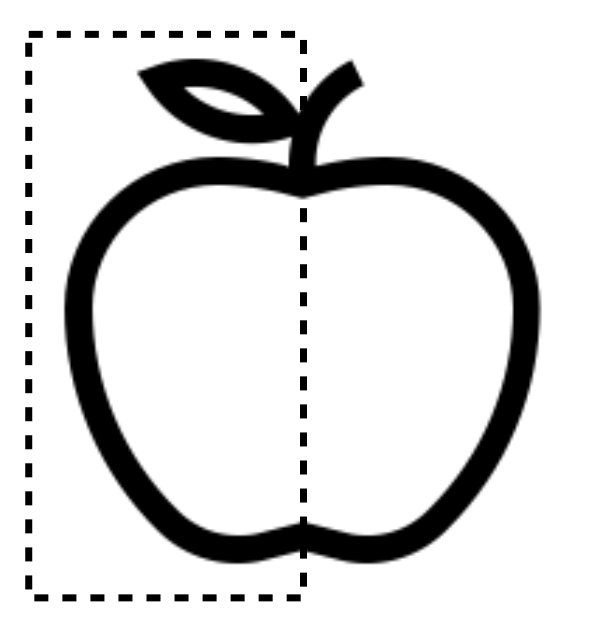
\includegraphics[scale=0.5]{figures/apple_cont-half.png}}
\ffigbox{\caption{Discontinuous half}\label{fig:apple_discont-half}}
        {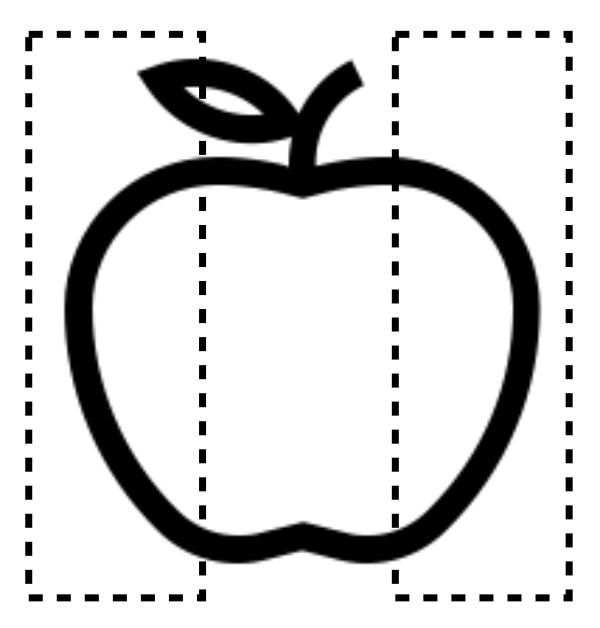
\includegraphics[scale=0.5]{figures/apple_discont-half.png}}
\end{floatrow}
\end{figure}


Let us now discuss possible extensions of proportional entity partitives involving \textit{pół}, \textit{połowa}, and \textit{połówka}. The phrases in \ref{ex:distribution-polowa-sg} (with \textit{połowa}) and \ref{ex:distribution-pol-sg} (with \textit{pół}) are true of both the object depicted in \figref{fig:apple_cont-half} and the entity in  \figref{fig:apple_discont-half}. Out of the blue, the continuous half reading is definitely the dominant one, however the discontinuous half interpretation can become salient in multiple contexts.\footnote{For most of the speakers I consulted the preferred reading of \ref{ex:distribution-polowa-sg} (with \textit{połowa}) is as in \figref{fig:apple_cont-half} though \figref{fig:apple_discont-half} is also possible. This preference seems to be much weaker in the case of \ref{ex:distribution-pol-sg} (with \textit{pół}).} For instance, it gets extremely relevant in a cooking scenario where pragmatically halves might be considered in terms of volume rather than individuated parts. Crucially, the ambiguity is systematic in entity partitives involving both \textit{połowa} and \textit{pół} and the sentences in \ref{ex:polish-half-words-pol-sentences} and \ref{ex:polish-half-words-polowa-sentences} are true both in a situation where the marked half in  \figref{fig:apple_cont-half} is red and when the designated portion in \figref{fig:apple_discont-half} is red. Now, it is quite intriguing that the partitive construction in \ref{ex:distribution-polowka-sg} (with \textit{połówka}) does not denote entities such as the one illustrated in \figref{fig:apple_discont-half}. Therefore, entity partitives with \textit{połówka} refer only to continuous integrated halves of an object denoted by the downstairs DP. Consequently, the sentence in \ref{ex:polish-half-words-polowka-sentences} would be judged true if the part indicated in \figref{fig:apple_cont-half} were red and false with respect to the portion in \figref{fig:apple_discont-half}.

\ex.\label{ex:polish-half-words-sentences} Polish
\ag. Pół jabłka jest czerwone.\label{ex:polish-half-words-pol-sentences}\\
half$_1$ apple\textsc{.gen} is red\\
`Half the apple is red.'
\bg. Połowa jabłka jest czerwona.\label{ex:polish-half-words-polowa-sentences}\\
half$_2$ apple\textsc{.gen} is red\\
`Half the apple is red.'
\bg. Połówka jabłka jest czerwona.\label{ex:polish-half-words-polowka-sentences}\\
half$_3$ apple\textsc{.gen} is red\\
`A half of the apple is red.'

A similar phenomenon can be observed in object position. In the sentences in \ref{ex:polish-half-words-sentences-object}, the partitives appear as arguments of a verb of consumption and as such denote an incremental theme \citep[see, e.g.,][]{dowty1991thematic,krifka1998origins,filip1999aspect,rothstein2003structuring}. Again, there is a contrast between \ref{ex:polish-half-words-pol-sentences-object} and \ref{ex:polish-half-words-polowa-sentences-object}, on the one hand, and \ref{ex:polish-half-words-polowka-sentences-object}, on the other, in terms of truth conditions. The first two sentences denote weaker propositions since for them to be judged true it would be enough for Marysia to eat a quantity of the apple in question corresponding approximately to 50\% of the apple's total volume. However, in many scenarios in which \ref{ex:polish-half-words-pol-sentences-object} and \ref{ex:polish-half-words-polowa-sentences-object} would be true the sentence in \ref{ex:polish-half-words-polowka-sentences-object} would not. This is because the proportional partitive headed by \textit{połówka} denotes a contiguous half, i.e., an integrated object within the whole as opposed to arbitrary portions of the apple mass. This stronger meaning results in that \ref{ex:polish-half-words-polowka-sentences-object} is true of a scenario such as the one illustrated in \figref{fig:apple_cont-half} and false with respect to \figref{fig:apple_discont-half}.

\ex.\label{ex:polish-half-words-sentences-object} Polish
\ag. Marysia zjadła pół jabłka.\label{ex:polish-half-words-pol-sentences-object}\\
Marysia ate half$_1$ apple\textsc{.gen}\\
`Marysia ate half the apple.'
\bg. Marysia zjadła połowę jabłka.\label{ex:polish-half-words-polowa-sentences-object}\\
Marysia ate half$_2$ apple\textsc{.gen}\\
`Marysia ate half the apple.'
\bg. Marysia zjadła połówkę jabłka.\label{ex:polish-half-words-polowka-sentences-object}\\
Marysia ate half$_3$ apple\textsc{.gen}\\
`Marysia ate a half of the apple.'

Furthermore, analogously to \textit{pół} proportional partitives involving \textit{połówka} and pluralia tantum get a part-of-a-singularity reading. The phrases in \ref{ex:pl.tantum-polowka-scissors} and \ref{ex:pl.tantum-polowka-dried-fruit} refer to halves of one object.\footnote{Some speakers report that \ref{ex:pl.tantum-polowka-scissors} is somewhat odd. I suspect that the reason is that scissors are not a kind of thing one normally divides into separate parts. My own intuition, however, is that though the phrase is certainly unusual, it is definitely interpretable and sounds absolutely natural in examples such as \ref{ex:polish-polowka-scissors-stabbing}.

\ex. Polish
\bg.[] Ofiara została zasztyletowana połówką nożyczek.\\
victim was stabbed half\textsubscript{3}\textsc{.ins} scissors\textsc{.gen}\\
`The victim was stabbed with a half of scissors.'\label{ex:polish-polowka-scissors-stabbing}

} In addition, similarly to the previously discussed examples a part yielded as a result of subatomic quantification has to be integrated. Thus, \ref{ex:pl.tantum-polowka-scissors} and \ref{ex:pl.tantum-polowka-dried-fruit} would be true of one scissor blade and, say, one continuous half of a raisin, respectively.\largerpage[2]

	\ex.\label{ex:pl.tantum-polowka} Polish
    \ag. \%połówka nożyczek\label{ex:pl.tantum-polowka-scissors}\\ 
	half$_3$ scissors\textsc{.gen}\\
	`a scissors half'
	\bg. połówka bakalii\label{ex:pl.tantum-polowka-dried-fruit}\\ 
	half$_3$ dried.fruit\textsc{.gen.pl}\\
	`a half of a dried fruit'

Given the non-trivial truth conditions of the sentence in \ref{ex:polish-half-words-polowka-sentences}, let us consider several naturally occurring examples involving entity partitives headed by the half-word \textit{połówka} from the National Corpus of Polish (NCP) \citep{przepiorkowski_et-al2012narodowy}, as given in \ref{ex:nkjp-polowka}.

\ex.\label{ex:nkjp-polowka} Polish (NCP)
\ag. [\dots] {zjadł [\dots]} połówkę sztokfisza.\label{ex:nkjp-polowka-cod}\\
{} he.ate half$_{3}$\textsc{.acc} dried.cod\textsc{.gen}\\
`[\dots] he ate [\dots] a half of a dried cod.'
\bg. [\dots] masz ochotę {na [\dots]} drink w połówce kokosa?\label{ex:nkjp-polowka-coconut}\\
{} you.have desire\textsc{.acc} on cocktail\textsc{.acc} in half$_{3}$\textsc{.loc} coconut\textsc{.gen}\\
`[\dots] would you like [\dots] a cocktail in a coconut half?'
\bg. [\dots] jesteśmy jak te dwie połówki jajka.\label{ex:nkjp-polowka-egg}\\
{} we.are like these two halves$_3$ egg\textsc{.gen}\\
`[\dots] we're like those two halves of an egg.'
\bg. [\dots] połówki {okna [\dots]} trzasnęły o ścianę.\label{ex:nkjp-polowka-window}\\
{} halves$_{3}$ window\textsc{.gen} banged about wall\textsc{.acc}\\
`[\dots] the window halves [\dots] banged on a wall.'
\bg. Otworzył portfel i {wyjął [\dots]} połówkę karty.\label{ex:nkjp-polowka-card}\\
he.opened wallet\textsc{.acc} and he.took.out half$_{3}$\textsc{.acc} card\textsc{.gen}\\
`He opened his wallet and took [\dots] a half of a card out of it.'

The first three examples in the sample, see \ref{ex:nkjp-polowka-cod}--\ref{ex:nkjp-polowka-egg}, involve reference to foodstuffs. The sentence in \ref{ex:nkjp-polowka-cod} would be true if the man in question consumed one half of a dried cod. Importantly, however, it would not be true in a situation where he ate, say, the tail and took some bites of the front left side and middle right side of the fish even if the total amount consumed equaled 50\% of the whole issue. The man had to eat either the left side or the right side of the cod or alternatively the half starting from the head or the half starting from the tail. Likewise, the question in \ref{ex:nkjp-polowka-coconut} makes reference to a half of a coconut coming in one piece, i.e., one would feel deceived if after answering ``yes'' they got several pieces of a coconut shell filled with portions of a cocktail they ordered. On the other hand, the use of \textit{połówka} in \ref{ex:nkjp-polowka-egg} is somewhat metaphorical. The inference here is that the speaker asserts that they and the addressee are like two individuated halves of an egg that fit well together. Again, the halves need to be continuous parts one receives after a clear horizontal or vertical cut. Yet another example is provided in \ref{ex:nkjp-polowka-window}. Here, however, the downstairs DP in the partitive does not refer to food but to a solid object of another type, i.e., a window consisting of two casements. The partitive phrase clearly implies that the halves in question are individuated and easily distinguishable parts, hence the casement window interpretation. Finally, the sentence in \ref{ex:nkjp-polowka-card} would be judged true only if the man in question took out a half of a card in one piece, i.e., it would necessarily be false if he took out several torn scraps of a card.

The discussion of \ref{ex:polish-half-words-polowka-sentences} as well as the attested examples from the National Corpus of Polish in \ref{ex:nkjp-polowka} leave no doubt that \textit{połówka} requires the referents of a partitive it occurs in to constitute an integrated part. Such a finding is quite remarkable and forces us to abandon the initial intuition that Polish half-words are semantically synonymous. The recapitulation of referential properties of explicit partitives involving the expressions in question is given in \tabref{tab:denotations-of-polish-half-words}. The main contrast between less marked \textit{połowa} and \textit{pół}, on the one hand, and more marked \textit{połówka}, on the other, lies in that the first two can designate discontinuous portions of stuff making up a whole, whereas the latter denotes only such divisions that constitute continuous, i.e., integrated, halves of an object.\footnote{According to many speakers, the semantics of \textit{połówka} is even stronger and indicates a half that is both integrated and symmetrical (or maybe at least comparable with the other half in terms of shape), i.e., the result of splitting is an object roughly along a line (or plane) of symmetry. However, since intuitions seem to be very subtle and not all speakers I consulted agree with the strong symmetrical requirement, I leave this issue for careful psycholinguistic experimentation to be pursued in the future.}

\begin{table}[h]
			\centering
			\begin{tabular}{lcc}
				\lsptoprule
				& \textsc{continuous part} & \textsc{discontinous part} \\ \midrule
				połowa  & $\checked$    & $\checked$      \\
				pół     & $\checked$    & $\checked$      \\
				połówka & $\checked$    & *                 \\ \lspbottomrule
			\end{tabular}
			\caption{Denotations of Polish half-words}\label{tab:denotations-of-polish-half-words}
		\end{table}

The novelty of the data introduced here is twofold. First of all, Polish half-words provide strong evidence that natural language is sensitive to the topological arrangement of parts of an entity. Second, the data imply that individuation is also possible at the subatomic level, i.e., quantification over parts in natural language reflects the fact that some parts might be assigned the status of an individual in its own right. In general, the distinction between different half-words in Polish can be described as follows. The least semantically marked expression \textit{połowa} is topologically neutral, i.e., the spatial make-up of an entity denoted by the downstairs DP in a partitive is irrelevant as long as it constitutes approximately 50\% of a whole. That is why \textit{połowa} does not discriminate between count singulars, plurals, and mass terms, and can felicitously appear in entity, set, and mass partitives. It simply separates out a half of whatever entity it is applied to. Furthermore, in this case subatomic quantification does not encode any constraints on what kind of entity is yielded. Hence, the result might be either a scattered entity such as a plurality or a discontinuous portion of matter. On the other hand, \textit{pół} and \textit{połówka} are topologically sensitive. They both require a DP they combine with to denote an integrated object, i.e., a cohesive whole. That explains why they cannot co-occur with expressions referring to scattered entities such as arbitrary sums of individuals or portions of a substance as typically denoted by plurals and mass nouns. The difference between the two is that \textit{pół} is similar to \textit{połowa} in that it does not impose any topological constraints on the resulting entity, whereas \textit{połówka} does. In other words, while \textit{pół} selects for an integrated object and returns either its continuous or discontinuous half, \textit{połówka} yields an integrated half of an integrated whole.

\subsection{Inherent vagueness}\label{sec:inherent-vagueness}
		
Similarly to other proportional quantifiers, expressions such as English \textit{half} appear to be inherently vague. Though disregarded by prescriptive grammars as an oxymoron, the concept of a bigger and smaller half is present in lexicons of many languages, as attested in the English, German, and Polish examples in \ref{ex:bigger-smaller-half-english}--\ref{ex:bigger-smaller-half-polish}. Interestingly, such phrases cannot be explained as bleached expressions meaning simply something like \textit{part}. For instance, for Polish speakers who would use or at least accept the NP in \ref{ex:bigger-half-polish}, i.e., speakers who have not internalized the linguistic prescription in question, it would be definitely true of a part constituting 55\% of a whole. However, it is unlikely that it would be judged true of 75\% of a whole and intuitively it seems definitely false of 90\% of a whole.

\ex.\label{ex:bigger-smaller-half-english} English
\a. \%bigger half\label{ex:bigger-half-english}
\b. \%smaller half\label{ex:smaller-half-english}

		\ex.\label{ex:bigger-smaller-half-german} German
        \ag. \%größere Hälfte\label{ex:bigger-half-german}\\
		bigger half\\
		`bigger half'
		\bg. \%kleinere Hälfte\label{ex:smaller-half-german}\\
		smaller half\\
		`smaller half'

		\ex.\label{ex:bigger-smaller-half-polish} Polish
        \ag. \%większa połowa\label{ex:bigger-half-polish}\\
		bigger half$_2$\\
		`bigger half'
		\bg. \%mniejsza połowa\label{ex:smaller-half-polish}\\
		smaller half$_2$\\
		`smaller half'

Given the possible interpretations discussed above, it seems plausible to assume that in natural language proportional quantifiers such as English \textit{half} denote a relation of constituting approximately 50\% share of a whole. In other words, their meaning is fuzzy in the sense that it allows for unequal parts as long as the disproportion falls within a particular range defined contextually.

\section{More topology-sensitive partitive words}\label{sec:more-topology-sensitive-partitive-words}

The observations made in \sectref{sec:continuous-discontinuous-parts} provide interesting evidence for certain semantic properties of natural language expressions that have not been recognized so far in the formal study of meaning. Nevertheless, a question might arise whether topological sensitivity is a marginal issue or whether it constitutes a broader phenomenon associated with a number of expressions in a language. Interestingly, it appears that half-words are not the sole category in Polish that displays the distinction between topological neutrality and topological sensitivity. In this section, I will examine more data from Polish partitive words indicating that the pattern is robust. 

\subsection{Quarter-words}\label{sec:quarter-words}

Let us first consider the contrasts between two other proportional partitives involving what I will refer to as quarter-words \textit{ćwierć} and \textit{ćwiartka} `quarter', as provided in \ref{ex:polish-quarter-words-morphology}. Analogously to \textit{połówka}, see \ref{ex:polish-half-polowka-morphology}, \textit{ćwiartka} is a morphologically complex expression derived from \textit{ćwierć} by the suffix \textit{-k-}.

		\ex. Polish\label{ex:polish-quarter-words-morphology}
        \ag. ćwierć-$\varnothing$\\
		root-inflectional.marker\\
		`quarter$_1$'\label{ex:polish-half-cwierc-morphology}
		\bg. ćwiart-k-a\\
		root-derivational.suffix$_1$-infl.marker\\
		`quarter$_2$'\label{ex:polish-half-cwiartka-morphology}

In terms of agreement, similarly to the distinction between \textit{pół} and \textit{połówka}, see \ref{ex:polish-half-words-agreement}, \textit{ćwierć} is neuter, whereas \textit{ćwiartka} triggers feminine agreement on adjectives and pronouns, as demonstrated in \ref{ex:polish-quarter-words-agreement}.\footnote{Similarly to \textit{pół}, some Polish speakers allow \textit{ćwierć} to combine with the demonstrative \textit{te} `these/this' (see fn. \ref{fn:plural-pol} and \citealt{przepiorkowski2006inherentnej}).}

\ex.\label{ex:polish-quarter-words-agreement} Polish
\ag. To czerwone ćwierć jabłka zgniło.\\
this\textsc{.nom.n} red\textsc{.nom.sg.n} quarter$_{1}$\textsc{.nom.n} apple\textsc{.gen.n} rotted\textsc{.sg.n}\\
`This red quarter of the apple got spoiled.'
\bg. Ta czerwona ćwiartka jabłka zgniła.\\
this\textsc{.nom.f} red\textsc{.nom.sg.f} quarter$_{2}$\textsc{.nom.f} apple\textsc{.gen.n} rotted\textsc{.sg.f}\\
`This red quarter of the apple got spoiled.'

The distribution of \textit{ćwierć} and \textit{ćwiartka} mimics the pattern observed in the \textit{pół} and \textit{połówka} alternation, i.e., both quarter-words appear to be sensitive to the type of nominal they combine with, see \ref{ex:distribution-cwierc} and \ref{ex:distribution-cwiartka}, respectively. In particular, as witnessed by the infelicity of the phrases in \ref{ex:distribution-cwierc-pl}--\ref{ex:distribution-cwierc-mass} as well as \ref{ex:distribution-cwiartka-pl}--\ref{ex:distribution-cwiartka-mass} neither of them occurs in set and mass partitives and only \textit{ćwierć} combines with collective nouns. Like \textit{połówka}, \textit{ćwiartka} typically combines with food terms or nominals denoting objects people usually cut into comparable pieces.\largerpage

		\ex.\label{ex:distribution-cwierc} Polish
        \ag. ćwierć jabłka\label{ex:distribution-cwierc-sg}\\
		quarter$_1$ apple\textsc{.gen}\\
		`quarter of the apple'
		\bg. ćwierć  stosu \minsp{(} jabłek)\label{ex:distribution-cwierc-group}\\
		quarter$_1$ pile\textsc{.gen} {} apples\textsc{.gen}\\
		`quarter of the pile of apples'
		\bg. \#ćwierć jabłek\label{ex:distribution-cwierc-pl}\\
		quarter$_1$ apples\textsc{.gen}\\
		Intended: `quarter of apples'
		\bg. \#ćwierć soku\label{ex:distribution-cwierc-mass}\\
		quarter$_1$ juice\textsc{.gen}\\
		Intended: `quarter of juice'

\ex.\label{ex:distribution-cwiartka} Polish
        \ag. ćwiartka jabłka\label{ex:distribution-cwiartka-sg}\\
		quarter$_2$ apple\textsc{.gen}\\
		`quarter of the apple'
		\bg. \#ćwiartka  stosu \minsp{(} jabłek)\label{ex:distribution-cwiartka-group}\\
		quarter$_2$ pile\textsc{.gen} {} apples\textsc{.gen}\\
		Intended: `quarter of the pile (of apples)'
		\bg. \#ćwiartka jabłek\label{ex:distribution-cwiartka-pl}\\
		quarter$_2$ apples\textsc{.gen}\\
		Intended: `quarter of the apples'
		\bg. \#ćwiartka soku\label{ex:distribution-cwiartka-mass}\\
		quarter$_2$ juice\textsc{.gen}\\
		Intended: `quarter of the juice'

This kind of behavior can be contrasted with a regular fraction expression such as \textit{jedna czwarta} `one-fourth', see \ref{ex:distribution-jedna-czwarta}. Unlike quarter-words or the half-words \textit{pół} and \textit{połówka}, fractions show no distributional constraints and can freely combine both with quantized predicates involving count singulars and with collectives and cumulative predicates such as plural nouns and mass terms.

\ex.\label{ex:distribution-jedna-czwarta} Polish
        \ag. {jedna czwarta} jabłka\label{ex:distribution-jedna-czwarta-sg}\\
		one-fourth apple\textsc{.gen}\\
		`one-fourth of the apple'
		\bg. {jedna czwarta}  stosu \minsp{(} jabłek)\label{ex:distribution-jedna-czwarta-group}\\
		one-fourth pile\textsc{.gen} {} apples\textsc{.gen}\\
		`one-fourth of the pile (of apples)'
		\bg. {jedna czwarta} jabłek\label{ex:distribution-jedna-czwarta-pl}\\
		one-fourth apples\textsc{.gen}\\
		`one-fourth of the apples'
		\bg. {jedna czwarta} soku\label{ex:distribution-jedna-czwarta-mass}\\
		one-fourth juice\textsc{.gen}\\
		`one-fourth of the juice'

Based on the distributional evidence, I posit that similarly to \textit{pół} and \textit{połówka} the quarter-words \textit{ćwierć} and \textit{ćwiartka} are topology-sensitive. Specifically, they quantify only over parts of integrated wholes. To put it differently, expressions having scattered entities such as arbitrary portions of matter or sums of individuals are disallowed as their input. On the other hand, fractions do not show such requirements and can yield a proportion of an entity of any kind. \tabref{tab:distribution-of-polish-quarter-words} summarizes the observations, namely the possibility of fraction entity, set, and mass partitives as opposed to the non-existence of proportional set and mass partitives headed by the quarter-words in Polish.

		\begin{table}[h]
			\centering
			\begin{tabular}{lccccc}
				\lsptoprule
				& \textsc{singulars} & \textsc{collectives} & \textsc{plurals} & \textsc{mass nouns} \\ \midrule
				jedna czwarta     & $\checked$ & $\checked$    & $\checked$ & $\checked$ \\
                ćwierć     & $\checked$ & $\checked$    & * & * \\
				ćwiartka & $\checked$ & * & * & * \\ \lspbottomrule
			\end{tabular}
			\caption{Distribution of Polish quarter-words}\label{tab:distribution-of-polish-quarter-words}
		\end{table}

\begin{sloppypar}
Moreover, the pattern is further corroborated by the differences in truth conditions of sentences involving fraction partitives and proportional partitives headed by \textit{ćwierć}, on the one hand, and proportional partitives headed by \textit{ćwiartka}, on the other. Analogously to the distinction discussed with respect to half-words, see \ref{ex:polish-half-words-sentences} and \ref{ex:polish-half-words-sentences-object}, there is a contrast in terms of possible verifications of \ref{ex:polish-quarter-words-fraction-sentences} and \ref{ex:polish-quarter-words-cwierc-sentences}, on the one hand, and \ref{ex:polish-quarter-words-cwiartka-sentences}, on the other. The first two sentences are true if any proportion of the apple constituting approximately 25\% of the whole apple is red regardless of whether it forms a discontinuous or continuous part. On the other hand, \ref{ex:polish-quarter-words-cwiartka-sentences} would only be true if an integrated quarter of the surface of the apple were red, i.e., similarly to sentences involving \textit{połówka} the partitive headed by \textit{ćwiartka} would not be true of a discontinuous part. 
\end{sloppypar}

\ex. Polish\label{ex:polish-quarter-words-sentences}
\ag. {Jedna czwarta} jabłka jest czerwona.\label{ex:polish-quarter-words-fraction-sentences}\\
one-fourth apple\textsc{.gen} is red\\
`One-fourth of the apple is red.'
\bg. Ćwierć jabłka jest czerwone.\label{ex:polish-quarter-words-cwierc-sentences}\\
quarter$_{1}$ apple\textsc{.gen} is red\\
`A quarter of the apple is red.'
\bg. Ćwiartka jabłka jest czerwona.\label{ex:polish-quarter-words-cwiartka-sentences}\\
quarter$_{2}$ apple\textsc{.gen} is red\\
`A quarter of the apple is red.'

Again, the same effect appears in object position. The incremental themes expressed by fraction partitives and proportional partitives with \textit{ćwierć} can refer either to continuous or discontinuous entities. Hence, the sentences \ref{ex:polish-quarter-words-fraction-sentences-object} and \ref{ex:polish-quarter-words-cwierc-sentences-object} would be true in a scenario where Marysia ate one piece of the apple as well as in a scenario where she took several unconnected bites constituting approximately 25\% of the total volume. In contrast, \ref{ex:polish-quarter-words-cwiartka-sentences-object} requires the theme of the verb of consumption to be an integrated object, i.e., it would be judged false in the second scenario.

\ex. Polish\label{ex:polish-quarter-words-sentences-object}
\ag. Marysia zjadła {jedną czwartą} jabłka.\label{ex:polish-quarter-words-fraction-sentences-object}\\
Marysia ate one-fourth apple\textsc{.gen}\\
`Marysia ate one-fourth of the apple.'
\bg. Marysia zjadła ćwierć jabłka.\label{ex:polish-quarter-words-cwierc-sentences-object}\\
Marysia ate quarter$_1$ apple\textsc{.gen}\\
`Marysia ate a quarter of the apple.'
\bg. Marysia zjadła ćwiartkę jabłka.\label{ex:polish-quarter-words-cwiartka-sentences-object}\\
Marysia ate quarter$_2$ apple\textsc{.gen}\\
`Marysia ate a quarter of the apple.'

Furthermore, examples naturally occurring in the NCP seem to corroborate the intuitions described above. The sentences in \ref{ex:nkjp-cwiartka-chicken} and \ref{ex:nkjp-cwiartka-baguette} involve reference to foodstuffs. The first does not report that the best meal in the place in question consisted of, say, fried chicken strips, but rather that the portion of meat was processed in one piece. In a similar vein, \ref{ex:nkjp-cwiartka-baguette} means that there was a continuous part of a baguette in a bag and not, e.g., several slices. Finally, \ref{ex:nkjp-cwiartka-paper} would be judged as false if what slided out were some scraps of a paper sheet.

\ex.\label{ex:nkjp-cwiartka} Polish (NCP)
\ag. Najlepsza tu kolacja: ćwiartka kurczaka [\dots]\label{ex:nkjp-cwiartka-chicken}\\
best here dinner quarter$_2$ chicken {}\\
`The best dinner here was a quarter of a chicken [\dots]'
\bg. {Biorę [\dots]} torebkę, w której leży {ćwiartka [\dots]} {bagietki [\dots]}\label{ex:nkjp-cwiartka-baguette}\\
I.take bag\textsc{.acc} in which\textsc{.loc} lies quarter$_2$ baguette\textsc{.gen}\\
`I'm taking a bag in which there is a quarter of a baguette [\dots]'
\bg. Ze środka wysunęła się ćwiartka papieru.\label{ex:nkjp-cwiartka-paper}\\
from interior\textsc{.gen} slided.out \textsc{refl} quarter$_2$ paper\textsc{.gen}\\
`A quarter of a paper sheet slided out from inside.'

The comparison of extensional properties of partitives involving fractions, \textit{ćwierć}, and \textit{ćwiartka} with regard to topological relations is given in \tabref{tab:denotations-of-polish-quarter-words}. The results show the very same pattern as discussed with regard to Polish half-words, see \tabref{tab:denotations-of-polish-half-words}.

\begin{table}[h]
			\centering
			\begin{tabular}{lcc}
				\lsptoprule
				& \textsc{continuous part} & \textsc{discontinous part} \\ \midrule
                jedna czwarta     & $\checked$    & $\checked$      \\				
                ćwierć     & $\checked$    & $\checked$      \\
				ćwiartka & $\checked$    & *                 \\ \lspbottomrule
			\end{tabular}
			\caption{Denotations of Polish quarter-words}\label{tab:denotations-of-polish-quarter-words}
		\end{table}

The comparison of Polish quarter-words with fractions mirrors the pattern observed for the distinction between topology-neutral and topology-sensitive half-words summarized in \tabref{tab:denotations-of-polish-half-words}. In the next section, I will discuss further evidence from partitive words.

\subsection{Piece-words}\label{sec:piece-words}

Another class of expressions displaying topological sensitivity consists of piece-words. Polish distinguishes between two such expressions, namely \textit{cząstka} and \textit{kawałek} `piece'. The first  is derived from the partitive word \textit{część} `part' by the suffix \textit{-k-}, compare \ref{ex:polish-piece-czesc-morphology} and \ref{ex:polish-piece-czastka-morphology}, whereas the second appears to be a basic form.\footnote{In fact, \textit{kawałek} is also morphologically complex and from a diachronic point of view it has been formed from \textit{kawał} `large share'. However, from the perspective of contemporary Polish, the relationship between the two is rather obscure and since the latter is semantically marked, it appears as if it were actually derived by means of the deletion of \textit{-ek-} from the first. This seems to be further corroborated by the fact that it is only possible to derive verbs from \textit{kawałek} and not from \textit{kawał}, e.g., \textit{kawałkować} `to portion' $\sim$ *\textit{kawałować}.} Similarly to English \textit{piece}, in many contexts \textit{kawałek} and \textit{cząstka} can be used interchangeably with the part-word \textit{część} though the former is a more frequent expression than the latter.\footnote{Another meaning of the noun \textit{cząstka} is `physical particle, corpuscule'. This meaning, however, will not be discussed here.} Nonetheless, like in other Polish partitive words also in this case there are some interesting topological properties worth discussing.\largerpage 
		
		\ex. Polish\label{ex:polish-piece-words-morphology}
        \ag. część-$\varnothing$\label{ex:polish-piece-czesc-morphology}\\
        root-inflectional.marker\\
        `part'
        \bg. cząst-k-a\label{ex:polish-piece-czastka-morphology}\\
		root-derivational.suffix-infl.marker\\
        `piece$_1$'
        \bg. kawałek-$\varnothing$\label{ex:polish-piece-kawalek-morphology}\\
        root-inflectional.marker\\
        `piece$_2$'

The distribution of the two expressions in question shows that they both resist combining with plural DPs, see \ref{ex:distribution-czastka-pl} and \ref{ex:distribution-kawalek-pl}. Furthermore, the infelicity of phrases such as \ref{ex:distribution-czastka-mass} and \ref{ex:distribution-kawalek-mass} suggests that both \textit{kawałek} and \textit{cząstka} impose the same topological restrictions on DPs they combine with as the partitive words \textit{pół}, \textit{połówka}, \textit{ćwierć}, and \textit{ćwiartka}, i.e., they disallow cumulative predicates denoting scattered entities.

  \ex. Polish\label{ex:distribution-czastka}
  \ag. cząstka jabłka\label{ex:distribution-czastka-sg}\\
  piece$_1$ apple\textsc{.gen}\\
  `piece of an apple'
  \bg. \# cząstka jabłek\label{ex:distribution-czastka-pl}\\
  piece$_1$ apples\textsc{.gen}\\
  Intended: `piece of apples'
  \bg. \# cząstka soku\label{ex:distribution-czastka-mass}\\
  piece$_1$ juice\textsc{.gen}\\
  Intended: `piece of juice'

  \ex. Polish\label{ex:distribution-kawalek}
  \ag. kawałek jabłka\label{ex:distribution-kawalek-sg}\\
  piece$_2$ apple\textsc{.gen}\\
  `piece of an apple'
  \bg. \# kawałek jabłek\label{ex:distribution-kawalek-pl}\\
  piece$_2$ apples\textsc{.gen}\\
  Intended: `piece of apples'
  \bg. \# kawałek soku\label{ex:distribution-kawalek-mass}\\
  piece$_2$ juice\textsc{.gen}\\
  Intended: `piece of juice'

Nevertheless, under closer inspection it turns out that in fact the piece-word \textit{kawałek} is not incompatible with all mass nouns but rather only with one particular class of such expressions. As witnessed in \ref{ex:distribution-mass-kawalek}, mass partitives headed by \textit{kawałek} are possible as long as the downstairs DP does not involve a liquid term, see \ref{ex:distribution-kawalek-mass-liquid}.\footnote{Gas terms are also infelicitous.} In particular, \textit{kawałek} can felicitously combine with mass expressions denoting solid substances as well as granular and artifactual aggregates.\footnote{Although examples such as \ref{ex:distribution-kawalek-mass-granular} and \ref{ex:distribution-kawalek-mass-fake} are not frequent and seem quite unusual, they are definitely interpretable and the intuitions regarding their meaning are clear. Notice also that a similar pattern is observed with respect to German \textit{Stück} `piece' as well as the diminutive forms such as \textit{Stückchen} and \textit{Stückerl} (Nina Haslinger, p.c.).} 

\ex. Polish\label{ex:distribution-mass-kawalek}
  \ag. \#kawałek wody\label{ex:distribution-kawalek-mass-liquid}\\
  piece$_2$ water\textsc{.gen}\\
  Intended: `piece of water'
  \bg. kawałek złota\label{ex:distribution-kawalek-mass-solid}\\
  piece$_2$ gold\textsc{.gen}\\
  `piece of gold'
  \bg. kawałek żwiru\label{ex:distribution-kawalek-mass-granular}\\
  piece$_2$ gravel\textsc{.gen}\\
  `piece of gravel'
  \bg. kawałek obuwia\label{ex:distribution-kawalek-mass-fake}\\
  piece$_2$ footwear\textsc{.gen}\\
  `piece of an item of footwear'

Interestingly, the partitive in \ref{ex:distribution-kawalek-mass-solid} does not simply refer to any portion of gold but rather to to an integrated (though most probably amorphous) lump, i.e., to a nugget. Likewise, the phrases in \ref{ex:distribution-kawalek-mass-granular} and \ref{ex:distribution-kawalek-mass-fake} have contiguous entities in their extension. Granular mass terms denote aggregates of objects such as grains of rice or granules of gravel that seem too small or not significant enough to be perceived as individuals in their own right \citep{grimm2012number,sutton_filip2016mass}. Instead, they are conceptualized as clusters of elements. As is well-known, those elements cannot be accessed by regular quantificational expressions such as distributive quantifiers or cardinal numerals, hence the possibility for granular concepts to be lexicalized as mass. However, the piece-word \textit{kawałek} in \ref{ex:distribution-kawalek-mass-granular} can access the part-whole structure of the granular and designate a single granule, i.e., a piece of gravel. 

Similarly, object mass nouns refer to stable discrete entities such as pieces of furniture or items of tableware \citep{gillon1992towards,chierchia1998plurality,chierchia2010mass,barner_snedeker2005quantity,bale_barner2009interpretation,rothstein2010counting,landman2011count}. Despite  their denotations, object mass nouns are uncountable, i.e., do not allow for quantification over individual objects they refer to. However, \textit{kawałek} yet again can reach the part-whole structure of an aggregate. Even more interestingly, it can quantify over parts of such discrete objects and trigger subatomic quantification, i.e., quantification over parts of a single item. As a result, \ref{ex:distribution-kawalek-mass-fake} can be interpreted as referring to a piece of a shoe. Admittedly, this effect appears to be marginal. However, it can be observed, e.g., in the attested fragment of discourse in \ref{ex:kawalek-mass-fake-attested}, where the phrase \textit{kawałek obuwia} `piece of an item of footwear' refers back to the noun \textit{obcas} `heel' showing clearly that the part-of-a-singularity interpretation is intended.\footnote{Source (accessed on 10th November 2020): \url{https://www.wattpad.com/525823126-troubles-up-your-sleeve-bellamy-blake-2-rozdzia\%C5\%82-2}.}

\ex. Polish (Internet)
\bg.[] Ale najpierw, oddaj \minsp{[} obcas]$_i$. -- Wyciągnął po niego rękę. Blondynka przełknęła cicho ślinę i wyciągnęła\hspace{3pt} \minsp{[} kawałek obuwia]$_i$ z rękawa [\dots]\\
but first give.back\textsc{.imp} {} heel\textsc{.acc} {} he.pulled.out for it\textsc{.acc} hand\textsc{.acc} blonde.woman swallowed silently saliva\textsc{.acc} and pulled.out {} piece\textsc{.acc} footwear\textsc{.gen} from sleeve\textsc{.gen} {}\\
`{``}But first, give me back the heel.'' He reached out for it. The blonde gulped silently and pulled out the piece of an item of footwear from her sleeve [\dots]'\label{ex:kawalek-mass-fake-attested}

The findings concerning the distribution of Polish piece-words in comparison to the part-word \textit{część} are summarized in  \tabref{tab:distribution-of-polish-piece-words}. Both \textit{cząstka} and \textit{kawałek} have a selectional restriction prohibiting them from combining with expressions denoting arbitrary sums of individuals, i.e., plurals. However, the main difference concerns the distribution with uncountable nouns. Unlike \textit{cząstka} which is generally incompatible with mass terms, \textit{kawałek} is sensitive to the properties of referents of a particular uncountable noun. In particular, it seems to require a certain stability of form so that parts singled out from a whole can sustain a fixed constant shape. In other words, \textit{kawałek} accepts entities displaying any kind of topological arrangement as long as it guarantees that the spatial form of pieces is relatively stable. This way it rejects liquid terms but can combine with expressions denoting solid substances, granular aggregates as well as artifacts, i.e., discrete entities related in terms of similar origin and functionality.

\begin{table}[h]
\centering
\begin{tabular}{lcccc}
\lsptoprule
\multirow{2}{*}{} & \multirow{2}{*}{\textsc{singulars}} & \multirow{2}{*}{\textsc{plurals}} & \multicolumn{2}{c}{\textsc{mass nouns}} \\
                  &                                                      &                                                    & liquids                  & others                        \\ \midrule
część             & $\checked$                                         & $\checked$                                       & $\checked$ & $\checked$                         \\
cząstka           & $\checked$                                         & *                                                  & * & *                                    \\
kawałek           & $\checked$                                         & *                                                  & *                        & $\checked$                  \\ \lspbottomrule
\end{tabular}
\caption{Distribution of Polish piece-words}\label{tab:distribution-of-polish-piece-words}
\end{table}

Another issue concerns the internal structure of objects denoted by partitives headed by piece-words. As provided in  \tabref{tab:denotations-of-polish-piece-words}, analogously to the partitive words \textit{połówka} and \textit{ćwiartka}, both \textit{cząstka} and \textit{kawałek} yield parts that can be recognized as contiguous integrated entities within a whole. This contrasts with the standard part-word \textit{część} which just like, e.g., the half-word \textit{połowa}, can deliver both continuous and scattered parts. What is especially interesting about \textit{kawałek} is that unlike \textit{połówka} and \textit{ćwiartka} it does not require the whole to be an integrated object. As long as it is not an arbitrary sum of individuals or a constantly deforming substance, \textit{kawałek} yields a portion of the whole that is one piece.

\begin{table}[h]
			\centering
			\begin{tabular}{lcc}
				\lsptoprule
				& \textsc{continuous part} & \textsc{discontinous part} \\ \midrule
                część    & $\checked$    & $\checked$      \\				
                cząstka     & $\checked$    & *      \\
				kawałek & $\checked$    & *                 \\ \lspbottomrule
			\end{tabular}
			\caption{Denotations of Polish piece-words}\label{tab:denotations-of-polish-piece-words}
		\end{table}

The properties of the piece-word \textit{kawałek} seem to relate to the scale of individuation proposed by \citet{grimm2012number}. However, there seems to be an interesting discrepancy. In \citeauthor{grimm2012number}'s original proposal, see \ref{ex:scale-of-individuation-original}, liquids and solid substances are grouped together with no ordering relation between them, i.e., \textit{water} falls into the same category as \textit{gold}. 

\ex. Fragment of the scale of individuation \citep[p. 80; adapted]{grimm2012number}\\
liquid/solid substance < granular aggregate < artifactual aggregate\dots\label{ex:scale-of-individuation}\label{ex:scale-of-individuation-original}

Yet the data concerning the distribution of the Polish piece-word \textit{kawałek} seem to suggest that an even more fine-grained distinction might be necessary to account for some grammatical phenomena in natural language. Since partitive phrases headed by \textit{kawałek} can only denote stable objects that come in one piece and are able to sustain their shape, they cannot combine with liquid terms such as \textit{water} simply because fluids continually deform, i.e., lack a given shape. Thus, it is possible that distinguishing between liquids and solid substances in terms of ordering on the scale of individuation, as proposed in \ref{ex:scale-of-individuation-modified}, might appear to be required.\footnote{It would be an interesting enterprise to explore whether there are more natural language expressions sensitive to the distinction between liquid and solid substance terms and if so whether that fact provides any interesting insights into the semantics of mass nouns. However, such a research project lies far beyond the scope of this study (for a discussion of related psychological evidence that infants can discriminate between solid objects and amorphous substances, see \sectref{sec:object-substance-distinction}).}

\ex. Modified fragment of the scale of individuation\\
liquid < solid substance < granular aggregate < artifactual aggregate\dots\label{ex:scale-of-individuation-modified}

Before we move on to discussing how the interplay of quantification and topology looks like from a cross-linguistic perspective and whether other languages can shed new light on the issues related to this phenomenon, let us briefly discuss the somewhat surprising fact that mass partitives are countable. In the next section, I will consider the relationship between substances and portions thereof.

\section{Mass, parts, quantities, and pieces}\label{sec:mass-parts-quantitifes-and-pieces}\largerpage

One of the very few attempts to link the issue of countability with partitivity and pseudo-partitivity \citep[see, e.g.,][]{selkirk1977some,koptjevskaja2001piece} has been pursued in \citet{chierchia2010mass}, who raises an interesting question concerning how it can be that one cannot count mass, whereas portions of mass are countable.\footnote{See also \citet{khrizman_et-al2015portion} and \citet{landman2016iceberg} for related considerations.} Specifically, how come expressions such as \ref{ex:mass-uncountable} and \ref{ex:mass-quantity-countable} can have a different status with respect to the mass/count distinction and yet refer to the very same entity.

 \ex. English (\citealt{chierchia2010mass}; adapted)\label{ex:mass-quantity}
 \a. That water is contaminated.\label{ex:mass-uncountable}
 \b. Those three quantities of water are contaminated.\label{ex:mass-quantity-countable} 

\citeauthor{chierchia2010mass} examines English relational expressions such as \textit{quantity}, \textit{part}, and \textit{piece} in partitive and pseudo-partitive constructions such as those in \ref{ex:quantity-chierchia}--\ref{ex:piece-chierchia} and observes a number of differences in their distribution.\footnote{A pseudo-partitive (sometimes called a quantitative), e.g.,\textit{a piece of cake}, differs from a partitive, e.g., \textit{a piece of that cake}, in that it does not indicate a part or a subset of an entity or a set, but rather it simply denotes either an amount of something or the number of members in a set.}

  	\ex. English (\citealt{chierchia2010mass}; adapted)\label{ex:quantity-chierchia}
  	\a. \jdg{(?)}a quantity of that person\label{ex:quantity-chierchia-sg}
  	\b. a quantity of apples\label{ex:quantity-chierchia-pl}   
	\b. two quantities of gold\label{ex:quantity-chierchia-mass}
    
    \ex. English (\citealt{chierchia2010mass}; adapted)\label{ex:part-chierchia}
	\a. a part of that person
	\b. \# a part of apples\label{ex:part-chierchia-pl}
	\b. \# a part of gold\label{ex:part-chierchia-mass}
    
    \ex. English (\citealt{chierchia2010mass}; adapted)\label{ex:piece-chierchia}
  	\a. a piece of that pizza\label{ex:piece-chierchia-sg}
  	\b. \# a piece of apples\label{ex:piece-chierchia-pl}
	\b. a piece of gold\label{ex:piece-chierchia-mass}

Though \textit{quantity} is slightly degraded with singular count nouns in entity partitives such as \ref{ex:quantity-chierchia-sg}, it combines felicitously with bare plurals and mass terms, see \ref{ex:quantity-chierchia-pl} and \ref{ex:quantity-chierchia-mass}, respectively. On the other hand, as we have already seen in \sectref{sec:entity-and-set-partitives-across-languages}, the English expression \textit{a part of} is incompatible with bare plurals, illustrated here by \ref{ex:part-chierchia-pl}. Moreover, it fails to take bare mass nouns as its complements, see \ref{ex:part-chierchia-mass}. Finally, \textit{piece} seems to fall somewhere in between the two categories since it can head partitives involving singular definite DPs like \ref{ex:piece-chierchia-sg} and bare mass nouns, as in \ref{ex:piece-chierchia-mass}, but cannot combine with bare plurals, see \ref{ex:piece-chierchia-pl}.

\citeauthor{chierchia2010mass} analyzes \textit{quantity}, \textit{part}, and \textit{piece} in terms of partitions imposing relative atomicity and non-overlap of members and attributes their selectional restrictions to the input requirements of the functions denoted by these expressions. Specifically, while \textit{quantity} is defined over properties of sums of entities, \textit{part} is defined over singular individuals and \textit{piece} displays a hybrid behavior.\footnote{I will return to \citeauthor{chierchia2010mass}'s proposal in \sectref{sec:doing-without-atoms}.} Although this approach is definitely thought-provoking, it seems that it misses an important point regarding the contrast between the expressions in question for at least two reasons. First, it neglects the role of topological sensitivity, as discussed above. But it also seems to ignore the distinction between counting and measuring \citep[see, e.g.,][]{rothstein2009individuating,rothstein2010counting,rothstein2011counting,rothstein2017semantics,partee_borschev2012sortal,khrizman_et-al2015portion,landman2016iceberg}. Intuitively, the difference between the two operations is that while counting is about specifying how many discrete objects of a certain kind there are, measuring determines some quantity in relevant units. To foreshadow, I will argue that counting is sensitive to topological characteristics such as being conceptualized as an integrated object, whereas measuring is not.\footnote{I will discuss the distinction between the two operations in detail in \sectref{sec:general-counting-principles}.} 

For a start, let us consider the count partitives in \ref{ex:quantity-chierchia-count} and \ref{ex:part-chierchia-count}.\footnote{Notice that a reviewer finds \ref{ex:part-chierchia-count} a bit awkward to interpret. Here, I ignore possible interspeaker variation and simply discuss the data, as reported by \citeauthor{chierchia2010mass}.} 

    \ex. English (\citealt{chierchia2010mass}; adapted)\label{ex:quantity-part-chierchia}
	\a. two quantities of that pizza\label{ex:quantity-chierchia-count}
	\b. two parts of that rice\label{ex:part-chierchia-count}

It seems that what happens in both cases is that at a certain level of the semantic derivation some sort of quantification in terms of volume is involved. The resulting measure is then subject to a shift that returns a count interpretation. In the literature, a number of operations that relate mass and count denotations have been proposed. For instance, one possibility is that the singular count noun \textit{pizza} in \ref{ex:quantity-chierchia-count} is shifted to the mass interpretation via the Universal Grinder \citep{pelletier1975nonsingular} or a similar operation and then the partitive word designates some amount of the mass before the entire phrase is shifted to a count denotation. Alternatively, the portion interpretation is derived via the measure interpretation by a special operator applied to the meaning of the partitive word \citep{khrizman_et-al2015portion}. Likewise, the part-word in \ref{ex:part-chierchia-count} could be paraphrased as \textit{portion} or \textit{proportion} and it essentially designates a particular volume of the rice in question.

Why is the distinction between counting and measuring of any significance here? Intuitively, quantities are about volume, pieces involve some form of individuation, i.e., are conceived of as independent objects, and parts can shift between these two aspects of quantification. However, to address this question more properly, let us consider the difference between the Polish part-word \textit{część} and piece-word \textit{kawałek}. Similarly to multiple other languages, Polish does not allow mass terms to combine with cardinal numerals (modulo coercion), see \ref{ex:mass-numerals}.

\ex. Polish\label{ex:mass-numerals}
  \ag. \#dwa złota\label{ex:mass-solid-numerals}\\
  two golds\\
  Intended: `two golds'
  \bg. \#dwa ryże\label{ex:mass-granular-numerals}\\
  two rices\\
  Intended: `two rices'

Interestingly, though, as witnessed in \ref{ex:mass-czesc-numerals}, mass partitives headed by \textit{część} are countable. In this case, the part-word gets a proportion interpretation, i.e., it measures the extension of the mass noun in terms of volume and indicates that the total volume is perceived as consisting of disjoint roughly equal sized quantities. For instance, the phrase in \ref{ex:czesc-mass-solid-numerals} designates two out of some number of more or less equally large amounts the total quantity of gold was divided into, irrespective of the size and shape of individual pieces of gold. Analogously, \ref{ex:czesc-mass-granular-numerals} indicates two comparable amounts out of the total amount of gravel.

\ex. Polish\label{ex:mass-czesc-numerals}
\ag. dwie części złota\label{ex:czesc-mass-solid-numerals}\\
  two parts gold\textsc{.gen}\\
  `two parts of the gold'
\bg. dwie części żwiru\label{ex:czesc-mass-granular-numerals}\\
  two parts gravel\textsc{.gen}\\
  `two parts of the gravel' 

On the other hand, the minimal pair examples involving the piece-word \textit{kawałek} in \ref{ex:mass-kawalek-numerals} lack the proportion reading, which suggests that the meaning of this expression does not merely concern quantification in terms of volume but rather it serves as a basis for counting individuated solid objects. Neither \ref{ex:kawalek-mass-solid-numerals} nor \ref{ex:kawalek-mass-granular-numerals} can get the volume interpretations available for \ref{ex:czesc-mass-solid-numerals} and \ref{ex:czesc-mass-granular-numerals}, respectively. They can only denote pluralities of pieces, i.e., solid integrated parts, of gold and gravel, respectively.\pagebreak

\ex. Polish\label{ex:mass-kawalek-numerals}
\ag. dwa kawałki złota\label{ex:kawalek-mass-solid-numerals}\\
  two pieces$_2$ gold\textsc{.gen}\\
  `two pieces of gold'
    \a. quantification in terms of objects
  \b. \#quantification in terms of volume
  \z.
\bg. dwa kawałki żwiru\label{ex:kawalek-mass-granular-numerals}\\
  two pieces$_2$ gravel\textsc{.gen}\\
  `two pieces of gravel'
  \a. quantification in terms of objects
  \b. \#quantification in terms of volume
  \z.

\begin{sloppypar}
To better illustrate the contrast, let us consider several natural sentences. Proportion uses of part-words are especially frequent in recipes and other cooking-related contexts. For instance, consider the examples in \ref{ex:recipes-czesc}, which are constructed based on typical recipes. Both in \ref{ex:recipes-czesc-mass} and \ref{ex:recipes-czesc-granular}, the count explicit partitives make reference to a particular volume of water and rice, respectively. 
\end{sloppypar}

\ex. Polish\label{ex:recipes-czesc}
\ag. Dolej do garnka dwie części wody, a w trzeciej namocz fasolę.\label{ex:recipes-czesc-mass}\\
you.pour\textsc{.imp} to pot\textsc{.gen} two\textsc{.acc} parts\textsc{.acc} water\textsc{.gen} and in third\textsc{.loc} you.soak\textsc{.imp} bean\textsc{.acc}\\
`Add two thirds of the water to the pot and soak the beans in the third part.'
\bg. Wymieszaj kaszę w proporcji 2:1, to znaczy dwie części ryżu na jedną część prosa.\label{ex:recipes-czesc-granular}\\
you.mix\textsc{.imp} porridge\textsc{.acc} in proportion\textsc{.loc} 2:1 this means two\textsc{.acc} parts\textsc{.acc} rice\textsc{.gen} on one\textsc{.acc} part\textsc{.acc} millet\textsc{.gen}\\
`Mix the porridge in the 2:1 ratio, which means two parts of rice for one part of millet.'

A similar effect can be observed in count partitives with plural nouns. For instance, consider the contrast in \ref{ex:recipes-czesc-kawalek}.\largerpage[2]

\ex. Polish\label{ex:recipes-czesc-kawalek}
\ag. Dwie części jabłek rozłóż równomiernie na blasze do pieczenia, a pozostałą część rozmiksuj.\label{ex:recipes-czesc-count}\\
two\textsc{.acc} parts\textsc{.acc} apples\textsc{.gen} you.put\textsc{.imp} evenly on tray\textsc{.loc} to baking\textsc{.gen} and remaining\textsc{.acc} part\textsc{.acc} you.blend\textsc{.imp}\\
`Put two thirds of the apples evenly on the baking tray and blend the remaining part.'
\bg.  Dwa kawałki jabłek rozłóż równomiernie na blasze do pieczenia, a pozostały kawałek rozmiksuj.\label{ex:recipes-kawalek-count}\\
two\textsc{.acc} pieces\textsc{.acc} apples\textsc{.gen} you.put\textsc{.imp} evenly on tray\textsc{.loc} to baking\textsc{.gen} and remaining\textsc{.acc} piece\textsc{.acc} you.blend\textsc{.imp}\\
`Put two apple pieces evenly on the baking tray and blend the remaining piece.'
  \a. quantification in terms of objects
  \b. \#quantification in terms of volume
  \z.

The count plural \textit{jabłka} `apples' in \ref{ex:recipes-czesc-count} is shifted to the mass denotation and the part-word \textit{część} quantifies over proportions of the apple mass making up the relevant apples and not over the apples as separate individuated objects. Whether the ingredients in question are stored as wholes or are cut into pieces plays no role for the truth conditions of the sentences in question. Consequently, if in response to \ref{ex:recipes-czesc-count} one apple was put on the baking tray and one half of an apple was blended or, alternatively, four apples were put on the baking tray and two apples were blended, the instruction would be followed correctly. Crucially, however, if we swap the part-word \textit{część} in \ref{ex:recipes-czesc-count} for the piece-word \textit{kawałek}, we get a significant contrast. Specifically, the sentence in \ref{ex:recipes-kawalek-count} cannot get a proportion reading, i.e., it cannot be understood as instructing one to put four apples on the baking tray and to blend the remaining two. Instead, it says you should put two integrated parts of different apples on the baking tray as well as blend one such part. Therefore, while the proportion interpretation of explicit partitives such as \ref{ex:mass-czesc-numerals} involves quantification in terms of volume along with the similarity in size restriction, piece-words do not trigger such a constraint.

In fact, English also allows for a proportion use of \textit{part} in numeral noun constructions when describing ratios, as in \ref{ex:ratio-part}.\footnote{The example in \ref{ex:ratio-part-plural} comes from a book by Rebecca Earle \textit{Feeding the people: The politics of the potato} (p. 93) accessed via Google. Source (accessed on 10th November 2020): \url{https://books.google.cz/books?id=WxzhDwAAQBAJ}.} This use is most natural with mass nouns, see \ref{ex:ratio-part-mass}, but it seems to work with plural count nouns too, as attested in \ref{ex:ratio-part-plural}.

\ex. English (Peter Sutton, p.c.)\label{ex:ratio-part}
\a. The ideal G\&T is four parts tonic to one part gin.\label{ex:ratio-part-mass}
\b. Potatoes constituted the core of the recipe, which required two parts of potatoes for every one of barley with dried peas.\label{ex:ratio-part-plural}

At this point, a preliminary conclusion can be drawn. The structure of parts can be such that it is merely a scattered entity, an unconnected configuration of bits related merely by virtue of belonging to the same whole. However, some parts are arranged in such a manner that they form a spatially contiguous entity that can be conceptualized as an individual in its own right. It appears that natural language is sensitive to this contrast and the Polish data show that this semantic distinction can be encoded formally in the lexicon. Although not every partitive word imposes topological restrictions regarding the spatial form of a portion of an entity the whole partitive construction denotes, there are some that do. Furthermore, it appears that counting and measuring differ with respect to topological properties of quantified entities. While the former operation requires integrated objects, the latter does not. 

The facts discussed above suggest that accounts that neglect the distinction in question most probably miss something crucial about how we humans conceptualize part-whole structures and how it relates to the phenomenon of countability in grammar. In the next section, I will inspect cross-linguistic evidence that further corroborates this claim.

\section{Cross-linguistic parallels}\label{sec:cross-linguistic-parallels}

Polish gives important insight into the role of topological notions in quantification over wholes and parts. However, one could wonder to what extent the semantic behavior of proportional partitives discussed above is a Polish idiosyncrasy. In this section, I will discuss cross-linguistic evidence suggesting that to\-po\-logy-sensitive expressions are a relatively widespread phenomenon in partitive constructions though not necessarily expressed by distinct lexical items. For instance, my informants report that the English sentences in \ref{ex:half-an-english} and \ref{ex:half-of-english} have different truth conditions. While the former is simply true in a scenario where 50\% of an apple was eaten by Mary, the meaning of the latter is stronger since it is true only if Mary ate a continuous half of an apple such as the one depicted in \figref{fig:apple_cont-half}.

\ex. English (Guy Tabachnick, p.c.)\label{ex:half-an-half-of-english}
\a. Mary ate half an apple.\label{ex:half-an-english}
\b. Mary ate a half of an apple.\label{ex:half-of-english}

However, the semantic difference between \ref{ex:half-an-english} and \ref{ex:half-of-english} is very slight and in multiple contexts it might be extremely hard to detect. Therefore, before we discuss data from English, German, Dutch, Brazilian Portuguese, and Mandarin, let us briefly elaborate on the method developed to tell an integrated-part and a scattered-part reading apart. For the sake of clarity, I will limit the discussion of subatomic topological sensitivity to proportional partitives involving half-words.

Since topological aspects of partitivity can be very subtle and intuitions in this respect tend to be somewhat obscure, in order to develop a proper diagnostic to detect topology-sensitive partitive expressions it seems necessary to come up with plain test objects readily divisible into comparable continuous and discontinuous parts differentiated by easily distinguishable properties. For instance, consider the flag test, as represented in \figref{fig:flag-AB} and \ref{fig:flag-ABA}. The Maltese-like flag in \figref{fig:flag-AB} consists of two continuous areas each constituting 50\% of the flag's surface. It is easy to distinguish between the halves since the left one is red whereas the right one is white. Therefore, the spatial arrangement of the parts fit what I will call an AB pattern. On the other hand, the red area in the Canadian-like flag illustrated in \figref{fig:flag-ABA} is discontinuous, i.e., it does not constitute an integrated half. I will call such an arrangement an ABA pattern.
		

\begin{figure}
\begin{floatrow}
\ffigbox{\caption{Flag AB}\label{fig:flag-AB}}
        {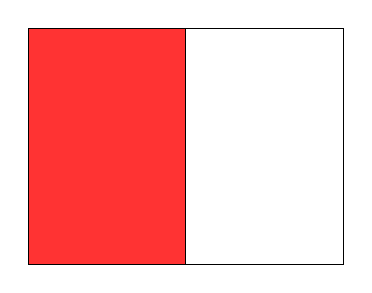
\begin{tikzpicture}
        \draw[fill=red!80] (0,0) -- (0,3) -- (2,3) -- (2,0) -- (0,0);
        \draw (2,3) -- (4,3) -- (4,0) -- (2,0) -- (2,3);
        \end{tikzpicture}}
\ffigbox{\caption{Flag ABA}\label{fig:flag-ABA}}
        {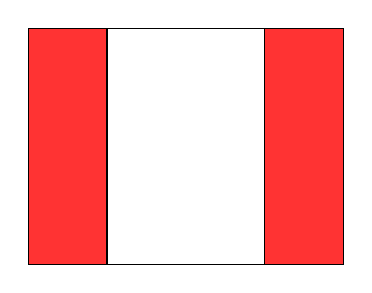
\begin{tikzpicture}
        \draw[fill=red!80] (0,0) -- (0,3) -- (1,3) -- (1,0) -- (0,0);
        \draw (1,3) -- (3,3) -- (3,0) -- (1,0) -- (1,3);
        \draw[fill=red!80] (3,3) -- (4,3) -- (4,0) -- (3,0) -- (3,3);
        \end{tikzpicture}}
\end{floatrow}
\end{figure}

As we saw in the previous sections, Polish encodes topological sensitivity lexically by differentiating between distinct partitive words. As in Polish, Brazilian Portuguese distinguishes between distinct half-words, namely \textit{metade} and \textit{meio} `half'. The former has nominal features and takes the partitive \textit{da}-phrase, whereas the latter is an adjectival expression agreeing with a modified noun in number and gender. Interestingly, similarly to Polish half-words \textit{metade} and \textit{meio} differ with respect to both their distributional and referential properties.\largerpage

Let us first consider the difference in the distribution of the two Brazilian Portuguese partitive expressions. While \textit{metade} patterns with \textit{połowa} in not being picky about the type of predicate within the \textit{da}-phrase it can combine with, see \ref{ex:distribution-metade}, \textit{meio} appears to correspond to \textit{pół} and \textit{połówka}. 

\ex. Brazilian Portuguese (Muriel Assmann, p.c.)\label{ex:distribution-metade}
\ag. metade da ma{\c{c}}{\~{a}}\label{ex:distribution-metade-sg}\\
half$_1$ the\textsc{.sg.f} apple\textsc{.f}\\
`half of the apple'
\bg. metade das ma{\c{c}}{\~{a}}s\label{ex:distribution-metade-pl}\\
half$_1$ the\textsc{.pl.f} apples\textsc{.f}\\
`half of the apples'
\bg. metade do suco\label{ex:distribution-metade-mass}\\
half$_1$ the\textsc{.sg.m} juice\textsc{.m}\\
`half of the juice'

As demonstrated in \ref{ex:distribution-meio-mass}, \textit{meio} cannot form a partitive with a mass term. Moreover, when combined with a plural noun it lacks a half-of-a-plurality reading, i.e., it cannot be interpreted as a quantifier over individuals making up the denoted plurality. Instead it can only operate on the subatomic level of particular members of the plurality denoted by a modified noun, i.e., it gets a half-of-a-singularity interpretation exclusively. In other words, \textit{meio} can only occur in an entity partitive and not in a set partitive. For instance, \ref{ex:distribution-meio-pl} cannot refer to a half of the total number of apples. The only interpretation available regards a plurality of apple halves.\largerpage

\ex. Brazilian Portuguese (Muriel Assmann, p.c.)\label{ex:distribution-meio}
\ag. meia ma{\c{c}}{\~{a}}\label{ex:distribution-meio-sg}\\
half$_{2}$\textsc{.sg.f} apple\textsc{.f}\\
`half of the apple'
\bg. meias ma{\c{c}}{\~{a}}s\label{ex:distribution-meio-pl}\\
half$_{2}$\textsc{.pl.f} apples\textsc{.f}\\
`apple halves'
\a. part-of-a-singularity reading
\b. \#part-of-a-plurality reading
\z. 
\bg. \#meio suco\label{ex:distribution-meio-mass}\\
half$_{2}$\textsc{.sg.m} juice\textsc{.m}\\
Intended: `half of the juice'

It seems plausible to posit that the contrasts between the phrases in \ref{ex:distribution-metade} and \ref{ex:distribution-meio} follow from topological restrictions imposed by \textit{meio} and \textit{metade} on what they select, analogously to the distinction between Polish \textit{pół} and \textit{połówka}, on the one hand, and \textit{połowa}, on the other. In other words, the nominal half-word \textit{metade} is topology-neutral, and thus can combine with DPs that denote integrated objects as well as those that have scattered entities in their extensions. On the other hand, adjectival \textit{meio} appears to be sensitive to the type of topological relations holding between parts of the referents of NPs it modifies. In particular, it requires integrated wholes. From a syntactic perspective, \textit{meio} as a nominal modifier sits lower in the structure than \textit{metade} which takes the whole DP as its complement. In other words, \textit{meio} is an adjective that is merged with the NP. Assuming that the NumP is higher than the AP \citep[e.g.,][]{ritter1991two,ritter1992cross}, this might explain scopal properties of \textit{meio} when it comes to subatomic quantification with respect to regular plurals, i.e., why \ref{ex:distribution-meio-pl} denotes a plurality of halves rather than half of a plurality. However, \textit{meio} can also combine with lexical plurals such as pluralia tantum, see \ref{ex:distribution-meio-pl.tant}, and it has been argued that the plural in lexical plurals is significantly lower, i.e., inside the \textit{n}P \citep[see, e.g.,][]{acquaviva2008lexical,alexiadou2011plural,smith2015feature,smith2017lexical}.\largerpage[2]

\ex. Brazilian Portuguese (Muriel Assmann, p.c.)
\bg.[] meio {\'{o}}culos\label{ex:distribution-meio-pl.tant}\\
half$_{2}$\textsc{.m} eye-glasses\textsc{.m}\\
`half of a pair of eye-glasses' or\\
`halves of eye-glasses'
\a. part-of-a-singularity reading
\b. \#part-of-a-plurality reading
\z.

Notice that \ref{ex:distribution-meio-pl.tant} gets a similar interpretation as the phrase in \ref{ex:distribution-meio-pl}, i.e., denotes a plurality of halves or rather, due to the number-neutrality of \textit{{\'{o}}culos} `eye-glasses', either a plurality of halves or one half of an object. I argue that this fact alongside the infelicity of phrases where \textit{meio} modifies mass terms, see \ref{ex:distribution-meio-mass}, supports the semantic explanation of the observed behavior in terms of topological sensitivity.

Even more interestingly, the results of the flag test show that \textit{meio} in fact patterns with Polish \textit{połówka}. As reported by my informant, the sentence with the proportional partitive with \textit{metade} in \ref{ex:flag-test-portuguese-metade} is true both in the flag AB scenario, see \figref{fig:flag-AB}, and in the flag ABA scenario, see \figref{fig:flag-ABA}. However, the sentence involving \ref{ex:flag-test-portuguese-meio} is judged true only in the former case and false in the latter. This means that \textit{metade} does not impose any topological restrictions on the portion of an entity denoted by the downstairs DP, wheres \textit{meio} yields only integrated parts.

		\ex. Brazilian Portuguese (Muriel Assmann, p.c.)\label{ex:flag-test-portuguese}
        \ag. Metade da bandeira é vermelha.\label{ex:flag-test-portuguese-metade}\\
		half$_1$ the flag is red\\
		`Half the flag is red.'
		\a. AB
		\b. ABA
		\z.
		\bg. Meia bandeira é vermelha.\label{ex:flag-test-portuguese-meio}\\
		half$_2$ flag is red\\
		`A half of the flag is red.'
		\a. AB
		\b. \#ABA
		\z.

A similar pattern is attested in Dutch where the distinction between the nominal expression \textit{helft} `half', on the one hand, see \ref{ex:flag-test-dutch-de-helft-van}, and adjectival \textit{half} `half', on the other, see \ref{ex:flag-test-dutch-halve}, is used in order to indicate the discussed contrast.\largerpage

\ex. Dutch (Erlinde Meertens, Izabela Jordanoska, p.c.)\label{ex:flag-test-dutch}
\ag. De helft van de vlag is rood.\label{ex:flag-test-dutch-de-helft-van}\\
		the half$_1$ of the flag is red\\
		`Half the flag is red.'
		\a. AB
		\b. ABA
		\z.
		\bg. De halve vlag is rood.\label{ex:flag-test-dutch-halve}\\
		the half$_2$ flag is red\\
		`A half of the flag is red.'
		\a. AB
		\b. \#ABA
		\z.

The half-word \textit{helft} forms a standard proportional entity partitive by combining with the prepositional \textit{van}-phrase which takes a singular DP as its complement (\citealt{de_hoop1997semantic,de_hoop2003partitivity}; see also \citealt[pp. 16--18]{cleven2013syntax}). On the other hand, Dutch \textit{half} resembles \textit{meio} in that it shows agreement with the modified NP. The suffix \textit{-e} on \textit{half} shows up when the noun is either definite or common gender, or both, as in the case of \ref{ex:flag-test-dutch-halve}, where it is spelled as \textit{halve}. As in the Brazilian Portuguese example, the flag test shows that \textit{helft} licenses both a continuous-half and a discontinuous-half interpretation, whereas adjectival \textit{half/halve} disallows the latter reading. In other words, while the sentence in \ref{ex:flag-test-dutch-de-helft-van} is reported to be true of both \figref{fig:flag-AB} and \ref{fig:flag-ABA}, \ref{ex:flag-test-dutch-halve} is judged false in the ABA flag scenario. This fact strongly suggests that Dutch lexicalized the distinction between topologically neutral and topologically sensitive partitive words. While \textit{helft} is similar to Polish \textit{połowa} or Brazilian Portuguese \textit{metade} in that it simply returns an entity constituting 50\% of a whole, truth conditions imposed by \textit{half/halve} are stronger, i.e., the partitive yields a half that needs to be integrated.  

It turns out that, as in Polish, Brazilian Portuguese and Dutch distinguish between topology-neutral and topology-sensitive half-words lexically. However, it is not the only way the distinction can be encoded in natural language. Thus, let us now consider a few strategies languages use to differentiate between the two partitive meanings in question that I identified in this chapter. Interestingly, different structures give rise to similar semantic effects concerning topological relations in subatomic quantification. The sample discussed here is relatively small, but the discussed data suggest that the observed semantic phenomenon is systematic and cross-linguistically valid. 

Let us start with the syntactic distinction occurring in English, as already mentioned in \ref{ex:half-an-half-of-english}. From a morphological point of view there is no contrast between the partitive word \textit{half} in \ref{ex:flag-test-english-half} and \ref{ex:flag-test-english-a-half-of}. Nevertheless, the syntactic structures in which it appears in each of the two sentences significantly differ (see \citealt{vannestal2004syntactic} for discussion). 
		
		\ex.\label{ex:flag-test-english} English (Jonathan Bobaljik, Jeffrey Parrott, p.c.)
        \a. Half the flag is red.\label{ex:flag-test-english-half}
		\a. AB
		\b. ABA
		\z.
		\b. A half of the flag is red.\label{ex:flag-test-english-a-half-of}
		\a. AB
		\b. \#ABA
		\z.

In \ref{ex:flag-test-english-half}, \textit{half} is a predeterminer since it can occur before regular determiners such as articles and demonstratives \citep[pp. 257--258]{quirk_greenbaum_leech_svartvik1985comprehensive}. On the other hand, in \ref{ex:flag-test-english-a-half-of} \textit{half} forms a standard proportional entity partitive by taking the \textit{of}-phrase with a singular DP as its complement. In this environment it seems to have nominal properties since it can be preceded by a determiner and it allows for numeral and adjectival modification \citep[p. 434]{huddleston_pullum2002cambridge}. The syntactic distinction translates into a semantic difference. Specifically, the sentence in \ref{ex:flag-test-english-half} is considered appropriate with respect to both the AB and ABA flag in \figref{fig:flag-AB} and \ref{fig:flag-ABA}, respectively, whereas \ref{ex:flag-test-english-a-half-of} would be judged true only in the first scenario.\footnote{A reviewer comments that they prefer \textit{one half of the flag} over \textit{a half of the flag} in this context. Though this raises an interesting question concerning interspeaker and/or dialectal variation, I ignore this issue here and simply report on my informants' judgments.} The contrast shows the relevance of topology in subatomic quantification even in the absence of distinct lexical items differentiating between a continuous-part and a discontinuous-part interpretation. In other words, it appears that natural language can employ purely syntactic means in order to indicate the notion of topological integrity of parts. Notice that the half-word in \ref{ex:flag-test-english-a-half-of} is preceded by the article. Superficially, the distinction between \textit{half} and \textit{a half of} resembles to some extent the contrast between the \textit{part}-expressions \textit{part of} and \textit{a part of}. The appearance of the indefinite article suggests that the latter should be treated on a par with count nominals and countability seems to imply spatial integrity.\largerpage

Another strategy is employed in German. At first blush, it might appear to pattern with Brazilian Portuguese and Dutch since it also distinguishes between the nominal half-word \textit{Hälfte} `half' and adjectival \textit{halb} `half'. However, German half-words display non-trivial interactions with determiners. While \textit{Hälfte} with the definite article \textit{die} shows similar behavior with respect to count singulars, plurals, and mass terms as Brazilian Portuguese \textit{metade}, see \ref{ex:distribution-halfte-def}, it is infelicitous with mass nouns when preceded by indefinite \textit{eine}, see \ref{ex:distribution-halfte}. 

\ex. German (Berit Gehrke, p.c.)\label{ex:distribution-halfte-def}
\ag. die Hälfte des Apfels\label{ex:distribution-halfte-sg-def}\\
the half$_1$ the\textsc{.gen} apple\textsc{.gen} \\
`half of the apple'
\bg. die Hälfte der Äpfel\label{ex:distribution-halfte-pl-def}\\
the half$_1$ the\textsc{.gen}  apples\textsc{.gen} \\
`half of the apples'
\bg. die Hälfte des Saftes\label{ex:distribution-halfte-mass-def}\\
the half$_1$ the\textsc{.gen}  juice\textsc{.gen} \\
`half of the juice'

\ex. German (Berit Gehrke, p.c.)\label{ex:distribution-halfte}
\ag. eine Hälfte des Apfels\label{ex:distribution-halfte-sg}\\
a half$_1$ the\textsc{.gen} apple\textsc{.gen} \\
`a half of the apple'
\bg. eine Hälfte der Äpfel\label{ex:distribution-halfte-pl}\\
a half$_1$ the\textsc{.gen}  apples\textsc{.gen} \\
`half of the apples'
\bg. \#eine Hälfte des Saftes\label{ex:distribution-halfte-mass}\\
a half$_1$ the\textsc{.gen}  juice\textsc{.gen} \\
Intended: `half of the juice'

On the other hand, definite DPs with adjectival \textit{halb} differ from Brazilian Portuguese phrases with \textit{meio} in that they can combine felicitously with all the types of expressions in question including mass nouns, see \ref{ex:distribution-halb-definite}. However, when preceded by the definite article, \textit{halb} is odd with mass nouns, and thus patterns with \textit{meio}, see \ref{ex:distribution-halb}.\largerpage

\ex. German (Nina Haslinger, p.c.)\label{ex:distribution-halb-definite}
\ag. der halbe Apfel\label{ex:distribution-halb-definite-sg}\\
the\textsc{.sg.m} half$_{2}$\textsc{.sg.m} apple\textsc{.m}\\
`the apple half'
\bg. die halben Äpfel\label{ex:distribution-halb-definite-pl}\\
the\textsc{.pl} half$_{2}$\textsc{.pl} apples\\
`the apple halves'
\a. part-of-a-singularity reading
\b. \#part-of-a-plurality reading
\z.
\bg. der halbe Saft\label{ex:distribution-halb-definite-mass}\\
the\textsc{.sg.m} half$_{2}$\textsc{.sg.m} juice\textsc{.m}\\
`half of the juice'

\ex. German (Nina Haslinger, p.c.)\label{ex:distribution-halb}
\ag. ein halber Apfel\label{ex:distribution-halb-sg}\\
a\textsc{.sg.m}  half$_{2}$\textsc{.sg.m} apple\textsc{.m}\\
`apple half'
\bg. halbe Äpfel\label{ex:distribution-halb-pl}\\
half$_{2}$\textsc{.pl}  apples\\
`apple halves'
\a. part-of-a-singularity reading
\b. \#part-of-a-plurality reading
\z.
\bg. \#halber Saft\label{ex:distribution-halb-mass}\\
half$_{2}$\textsc{.sg.m} juice\textsc{.m} \\
Intended: `half of the juice'

In addition, the examples with the definite article in \ref{ex:distribution-halb-definite} seem to also have an additional expressive intensifier reading of the sort `all those apples'. For instance, it would be appropriate when half of the apples were splattered across the street and the speaker were expressive about this situation (somewhat like \textit{totally}).\footnote{I would like to thank Berit Gehrke for sharing this observation with me.}\largerpage

The facts discussed above suggest that whether \textit{Hälfte} and \textit{halb} are sensitive to the spatial constitution of referents of the NP they attach to depends on the determiner. In particular, their selectional restrictions suggest that German definite DPs with half-words are topology-neutral, whereas their indefinite counterparts are topology-sensitive. The results of the flag test seem to support that idea. As witnessed in \ref{ex:flag-test-german-halfte} and \ref{ex:flag-test-german-halb}, sentences with definite DPs involving \textit{Hälfte} and \textit{halb} are judged true in both the AB and the ABA flag scenario. Unlike in the case of Brazilian Portuguese \textit{meio}, there is no contrast between \textit{Hälfte} and the expressive reading of \textit{halb} with respect to the the spatial make up of the partial entity they yield here.\footnote{Note, however, that \ref{ex:flag-test-german-halb} has also a strongly individuating reading that there is one piece of cloth, which is half a flag (the other half is ripped off), and that half-flag is red.}

\ex. German (Berit Gehrke, Nina Haslinger, Maximilan Prüller, p.c.)\label{ex:flag-test-german}
\ag. Die Hälfte der Fahne ist rot.\label{ex:flag-test-german-halfte}\\
		the half$_1$ the\textsc{.gen} flag is red\\
		`Half the flag is red.'
		\a. AB
		\b. ABA
		\z.
		\bg. Die halbe Fahne ist rot.\label{ex:flag-test-german-halb}\\
		the half$_2$ flag is red\\
		`Half the flag is red.'
		\a. AB
		\b. ABA
		\z.

Now, consider the indefinite counterparts of \ref{ex:flag-test-german} in \ref{ex:flag-test-german-indef}. Both \ref{ex:flag-test-german-halfte-indef} and \ref{ex:flag-test-german-halb-indef} display the kind of semantic behavior observed in typologically sensitive expressions such as Polish \textit{połówka}, Brazilian Portuguese \textit{meio}, and Dutch \textit{half}, i.e., they would be true only if a continuous part of the flag were red.\footnote{Again, the non-expressive reading of \ref{ex:flag-test-german-halb-indef} is that there is a half of the flag that is cut off or separated from the rest.} This shows that the source of topological sensitivity is the interaction between the half-word and the determiner rather than that it is encoded lexically.  

\ex. German (Berit Gehrke, p.c.)\label{ex:flag-test-german-indef}
\ag. Eine Hälfte der Fahne ist rot.\label{ex:flag-test-german-halfte-indef}\\
a half$_1$ the\textsc{.gen} flag is red\\
`A/One half of the flag is red.'
		\a. AB
		\b. \#ABA
		\z.
\bg. Eine halbe Fahne ist rot.\label{ex:flag-test-german-halb-indef}\\
a half$_2$  flag is red\\
`One piece, which is half a flag, is red.'
		\a. AB
		\b. \#ABA
		\z.

Furthermore, there is yet another topology-sensitive construction in German. In particular, consider the subject of the sentence in \ref{ex:german-eine-halfte-definite-article} involving the half-word \textit{Hälfte} preceded by both what at first blush appears to be an indefinite article and the definite article \textit{die}. Notice, however, that \textit{eine} in this environment is not an indefinite article, but rather the numeral `one'. The mere fact that it can combine with the definite article \textit{die} suggests that it is an expression of a different type. Furthermore, unlike regular indefinite articles, it is always stressed. As shown by the ungrammaticality of \ref{ex:german-halfte-stress}, in this construction one cannot put stress on the half-word.\largerpage

\ex. German (Berit Gehrke, Maximilian Prüller, p.c.)\label{ex:german-eine-halfte}
\ag. Die EINE Hälfte der Fahne ist rot.\label{ex:german-eine-halfte-definite-article}\\
the one half$_1$ the\textsc{.gen} flag is red.\\
`The half of the flag is red.'
\bg. *Die eine HÄLFTE der Fahne ist rot.\label{ex:german-halfte-stress}\\
the a half$_1$ the\textsc{.gen} flag is red.\\
Intended: `The half of the flag is red.'

The truth conditions of sentences with the \textit{die eine Hälfte} partitive expression contrast with the truth conditions of the sentences involving definite proportional partitives examined so far. For instance, consider \ref{ex:flag-test-german2}.  

\ex. German (Berit Gehrke, Nina Haslinger, Maximilan Prüller, p.c.)\label{ex:flag-test-german2}
\ag. Die Hälfte der Fahne ist rot.\label{ex:flag-test-german-die-halfte}\\
		the half$_1$ the.\textsc{gen} flag is red\\
		`Half the flag is red.'
		\a. AB
		\b. ABA
		\z.
		\bg. Die eine Hälfte der Fahne ist rot.\label{ex:flag-test-german-die-eine-halfte}\\
		the a/one half$_1$ the\textsc{.gen} flag is red\\
		`One half of the flag is red.'
		\a. AB
		\b. \#ABA
		\z.

As we have already discussed, \ref{ex:flag-test-german-die-halfte} is true of both relevant scenarios, i.e.,  \figref{fig:flag-AB} and \ref{fig:flag-ABA}. However, \ref{ex:flag-test-german-die-eine-halfte} is consistently judged false in the flag ABA situation. This shows that German developed a rather complex system in which the semantic distinction between different proportional partitive expressions, i.e., topologically neutral partitives, on the one hand, and topology-sensitive expressions, on the other, results from the interaction between the half-word, definiteness, and the numeral. The expressions are distinguished from each other both lexically and structurally with the most marked form being at the same time  semantically most complex.

Finally, the examined contrast involving yet another two types of constructions is found in Mandarin. The two structures are provided in \ref{ex:flag-test-mandarin}. 

		\ex. Mandarin (Chang Liu, p.c.)\label{ex:flag-test-mandarin}
        \ag. gu{\'{o}} q{\'{i}} de y{\'{i}}-b{\`{a}}n sh{\`{i}} h{\'{o}}ng de.\label{ex:flag-test-mandarin-yiban}\\
		national flag \textsc{lnk} one-half \textsc{cop} red \textsc{lnk}\\
		`Half the national flag is red.'
		\a. AB
		\b. ABA
		\z.
		\pagebreak\bg. b{\`{a}}n-mi{\`{a}}n gu{\'{o}} q{\'{i}} sh{\`{i}} h{\'{o}}ng de.\label{ex:flag-test-mandarin-banmian}\\
		half-\textsc{clf} national flag \textsc{cop} red \textsc{lnk}\\
		`A half of the national flag is red.'
		\a. AB
		\b. \#ABA
		\z.

In \ref{ex:flag-test-mandarin-yiban}, the partitive meaning is conveyed by the phrase involving the proportional expression \textit{y{\'{i}}-b{\`{a}}n} `half' related by the associative marker \textit{de} to the nominal \textit{gu{\'{o}} q{\'{i}}} `national flag' (\citealt[p. 294]{jing-schmidt2005dramatized}; \citealt{jin2018partition}). In this construction, the half-word \textit{b{\`{a}}n} does not follow a classifier and combines directly with the preceding cardinal numeral \textit{y{\'{i}}} `one' forming a constituent. It is possible that \textit{y{\'{i}}} in \textit{y{\'{i}}-b{\`{a}}n} is in fact a grammaticalized expression interpreted as an indefinite rather than a numeral (see \citealt[p. 127]{hsieh2008internal}; \citealt{jin2018partition}).\footnote{See also \citet[p. 46]{hsieh2008internal} and \citet{zhang2011constituency} for the discussion of issues regarding constituency and other types of environments \textit{b{\`{a}}n} appears in.} In any case, this structure is topologically neutral and yields both integrated and discontinuous halves of entities since sentences such as \ref{ex:flag-test-mandarin-yiban} are reported to be true of the flag in \figref{fig:flag-AB} as well as the one in \figref{fig:flag-ABA}. In \ref{ex:flag-test-mandarin-banmian}, however, the partitive morpheme \textit{b{\`{a}}n} behaves more like a quantifier since it needs to combine with the classifier \textit{mi{\`{a}}n} dedicated to counting flat and smooth objects such as mirrors in order to quantify over parts of the national flag denoted by the nominal. Therefore, it appears that in this case the syntactic status of the half-word is on a par with cardinals. And again, a different structure corresponds to a different semantics. Unlike \ref{ex:flag-test-mandarin-yiban}, the sentence in \ref{ex:flag-test-mandarin-banmian} can only mean that an integrated half of the national flag is red, i.e., it would be judged false in the scenario represented in \figref{fig:apple_discont-half}.

The Mandarin example discussed above concludes this brief exploration of cross-linguistic strategies of encoding sensitivity to topological notions in partitive expressions. Though the sample of languages examined here was relatively small and most probably more strategies await to be discovered within a future thorough cross-linguistic investigation, the presented evidence proves that natural language encodes subtle topological distinctions in the domain of partitivity. The contrasts examined here are often very slight but a careful examination suggests that the topology-related phenomena in question are not something idiosyncratic but rather occur systematically across languages.

In the next section, I will discuss yet another class of expressions that might shed new light on the issues related to the interplay of quantification and topology. In particular, I will consider some similarities and contrasts concerning two whole-adjectives in Polish, namely \textit{cały} `whole' and \textit{kompletny} `complete'. To this end, I will explore two different respects of being entire as well as the interaction between whole-adjectives and different types of nominals from the perspective of subatomic quantification and topological sensitivity.

\section{Whole-adjectives}\label{sec:whole-adjectives}

Due to contrasts parallel to the one illustrated in \ref{ex:whole-adjectives-ferret}, adjectives such as \textit{whole} and \textit{entire} have been analyzed as universal quantifiers over parts \citep{moltmann1997parts} or maximizing modifiers, i.e., expressions restricting exception tolerance \citep{morzycki2002wholes}.\footnote{\citet{morzycki2002wholes} builds on \citeposst{brisson1998distributivity} analysis of \textit{all} in terms of maximizing modification.} There is a strong intuition that compared to \ref{ex:ferret} the sentence in \ref{ex:whole-ferret} implies that no part of the entity in question is exempt from having to satisfy the main predicate. In particular, \ref{ex:ferret} would be true if a sufficiently significant proportion of the ferret were under the water, i.e., if part of a paw or a tail were not submerged, under most circumstances the sentence would not be considered false. However, the proposition expressed by \ref{ex:whole-ferret} is stronger. It states that all the parts of the ferret are submerged.

\ex. English (\citealt{morzycki2002wholes}; adapted)\label{ex:whole-adjectives-ferret}
\a. The ferret is submerged.\label{ex:ferret}
\b. The \{whole/entire\} ferret is submerged.\label{ex:whole-ferret}

In Polish, alongside the standard whole-adjective \textit{cały} `whole', there is yet another expression that shares some of its semantic properties yet differs in an interesting respect, namely the adjective \textit{kompletny} `complete'. Though there is a partial overlap between the two expressions in question in terms of their distribution, they show quite different patterns. 

Let us first consider the distributional potential of the whole-adjective \textit{cały}. What is interesting about this expression is that it can be used for universal quantification over parts of stuff denoted both by singular count nouns and mass terms. Specifically, \ref{ex:distribution-caly-sg} refers to all the material parts making up a particular apple, whereas \ref{ex:distribution-caly-mass} is true of an entity comprising all the quantities of juice in a relevant context, i.e., the total amount of juice. Interestingly, when modifying a plural expression such as \ref{ex:distribution-caly-pl}, in some contexts \textit{cały} can scope over the plural. In other words, \ref{ex:distribution-caly-pl} is true of a plurality of whole apples but it can also be true of a whole plurality of not necessarily whole apples.\largerpage[-1]\pagebreak

		\ex. Polish\label{ex:distribution-caly}
        \ag. całe jabłko\label{ex:distribution-caly-sg}\\
		whole\textsc{.sg.n} apple\textsc{.n}\\
		`whole apple' or\\`all (of) the apple'
        \bg. cały sok\label{ex:distribution-caly-mass}\\
		whole\textsc{.sg.m} juice\textsc{.m}\\
		`all (of) the juice'
		\bg. całe jabłka\label{ex:distribution-caly-pl}\\
		whole\textsc{.pl} apples\\
		`whole apples' or\\`all (of) the apples'
        \a. plural > whole
        \b. whole > plural
        \z.

Admittedly, the cases in which \textit{cały} can outscope the plural are restricted and in many environments such a reading is either unavailable or marked. However, there are contexts in which it is definitely possible. One such example is illustrated by the sentence in \ref{ex:caly-scope}.

\ex. Polish (Adam Przepiórkowski, p.c.)\label{ex:caly-scope}
\bg.[] Szczury zjadły całe jabłka, choć większość {i tak} była już wcześniej nadgryziona przez myszy.\\
rats ate whole\textsc{.acc} apples\textsc{.acc} though most anyway was already earlier nibbled by mice\textsc{.acc}\\
`Rats ate all of the apples, although most of them were already nibbled off by mice.'
		
Compared to \textit{cały}, the distribution of \textit{kompletny} is significantly restricted. Intuitively, this is due to the fact that it seems to presuppose a certain complexity in terms of a part-whole structure. In particular, it can only modify nominals referring to objects consisting of multiple easily recognizable and distinguishable parts such as utensils and clothes.\footnote{There is yet another meaning of \textit{kompletny} that could be glossed as `total' which does not impose such a constraint. This use is especially frequent in colloquial Polish; however, it will not be considered here.} 

In addition to this restriction, the whole-adjective \textit{kompletny} differs from \textit{cały} in that it can never scope over the plural. For instance, due to the fact that computers consist of many detachable elements, \ref{ex:distribution-kompletny-sg} is a meaningful phrase in Polish. Similarly, when combined with an object mass term it implies that all discrete objects comprising the extension of the noun are in place. For example, \ref{ex:distribution-kompletny-mass} would be true of a collection of equipment where there is no item missing. Moreover, \textit{kompletny} frequently appears with collective nouns such as \textit{zestaw} `set' and \textit{kolekcja} `collection', which denote groups of artifacts. On the other hand, when modifying a plural expression, as in \ref{ex:distribution-kompletny-pl}, \textit{kompletny} cannot assert the denoted property of a plurality as such, but rather of singular individuals. In other words, \ref{ex:distribution-kompletny-pl} means that individual computers are complete and not the plurality thereof.

		\ex. Polish\label{ex:distribution-kompletny}
        \ag. kompletny komputer\label{ex:distribution-kompletny-sg}\\
		complete\textsc{.sg.m} computer\textsc{.m}\\
		`complete computer'
        \bg. kompletny sprzęt\label{ex:distribution-kompletny-mass}\\
		complete\textsc{.sg.m} equipment\textsc{.m}\\
        `complete equipment'
		\bg. kompletne komputery\label{ex:distribution-kompletny-pl}\\
		complete\textsc{.pl} computers\\
		`complete computers'
        \a. plural > complete
        \b. \#complete > plural
        \z.

Notice also that both \textit{cały} and \textit{kompletny} can combine with pluralia tantum, see \ref{ex:caly-pl.tant}--\ref{ex:kompletny-pl.tant}. The plurale tantum nominal \textit{nożyczki laparaskopowe} `laparoscopic graspers' denotes a specialized object consisting of multiple detachable and replaceable elements, which makes it a proper expression to be modified by \textit{kompletny}. In both cases, the whole phrase is ambiguous between a singular and a plural reading, i.e., it either refers to one whole or complete object, respectively, or to a plurality of whole or complete objects. 

\ex. Polish\label{ex:calykompletny-pl.tant}
\ag. całe nożyczki laparoskopowe\label{ex:caly-pl.tant}\\
whole\textsc{.pl} scissors laparoscopic\textsc{.pl}\\
`whole laparoscopic graspers' or\\
`all of the laparoscopic graspers'
\bg. kompletne nożyczki laparoskopowe\label{ex:kompletny-pl.tant}\\
complete\textsc{.pl} scissors laparoscopic\textsc{.pl}\\
`complete laparoscopic graspers'

The reading on which the whole-adjective would impose a semantic restriction on a plurality can be available only for \ref{ex:caly-pl.tant}, i.e., only this phrase can mean something like a whole plurality of laparoscopic graspers. This can be observed in a shopping context, where a sentence such as \ref{ex:caly-pl.tant-scope} means that the owners of the store ran out of laparoscopic gaspers. Given the fact that the plural in plurale tantum nouns was argued to be inside the \textit{n}P \citep[see, e.g.,][]{acquaviva2008lexical,alexiadou2011plural,smith2015feature,smith2017lexical}, data like \ref{ex:caly-pl.tant-scope} suggest that \textit{cały} can enter into a scopal relation with a plurality even when it is encoded very low in the structure.

\ex. Polish\label{ex:caly-pl.tant-scope}
\bg.[] Dziś było tyle zamówień ze szpitali, że sprzedaliśmy całe nożyczki laparoskopowe.\\
today was so.many orders\textsc{.gen} from hospitals\textsc{.gen} that we.sold whole\textsc{.pl} scissors laparoscopic\textsc{.pl}\\
`Today there were so many orders from hospitals that we sold out all laparoscopic graspers.' 

\tabref{tab:distribution-of-polish-whole-adjectives} gives an overview of the distribution of the Polish whole-adjectives \textit{cały} and \textit{kompletny} as discussed above. While both can co-occur with singular count nouns and mass terms, the latter requires the modified noun to refer to complex entities consisting of multiple easily individuated parts. On the other hand, when combined with regular plurals, only \textit{cały} can scope over the plural. In other words, what is targeted by \textit{kompletny} is always the part-whole structure of a particular singular individual, whereas \textit{cały} in some cases can trigger universal quantification over singular objects making up a plural entity. 

		\begin{table}[h]
			\centering
			\begin{tabular}{lcccccc}
				\lsptoprule
				& \textsc{singulars} & \textsc{mass nouns}   & \textsc{plurals} \\ \midrule
				cały & $\checked$  & $\checked$    & $\checked$            \\ 
				kompletny & $\checked$    &  $\checked$    & \#            \\
				\lspbottomrule
			\end{tabular}
			\caption{Distribution of Polish \textit{whole} adjectives}
            \label{tab:distribution-of-polish-whole-adjectives}
		\end{table}

The evidence regarding the distribution of the Polish whole-adjectives in question suggests the distinction between integrated objects as prototypically denoted by singular count nouns and scattered entities designated by mass terms, on the one hand, and arbitrary sums of individuals referred to plural expressions, on the other. To some extent this contrast resembles what was observed with respect to the distribution of the piece-word \textit{kawałek} in \sectref{sec:piece-words} and \sectref{sec:mass-parts-quantitifes-and-pieces}. Before I move on to discussing some semantic differences between \textit{cały} and \textit{kompletny}, let us briefly examine a cross-linguistic context which might shed more light on the pattern observed in Polish. In the next section, I will consider data concerning a German whole-adjective modifying plural nouns.

\subsection{German \textit{ganz} and plurals}\label{sec:german-ganz-and-plurals}

As in Polish, in German the whole-adjective \textit{ganz} `whole' can be used as a universal quantifier over parts of matter making up referents of both singular count nouns as well as mass terms, as demonstrated in \ref{ex:distribution-ganz-sg}--\ref{ex:distribution-ganz-mass} \citep[see also][pp. 123--127]{moltmann1997parts}.

\ex. German (Nina Haslinger, p.c.)\label{ex:distribution-ganz}
        \ag. der ganze Apfel\label{ex:distribution-ganz-sg}\\
		the\textsc{.sg.m} whole\textsc{.sg} Apfel\textsc{.m}\\
		`the whole apple' or\\`all (of) the apple'
        \bg. der ganze Saft\label{ex:distribution-ganz-mass}\\
		the\textsc{.sg.m} whole\textsc{.sg} juice\textsc{.m}\\
        `all (of) the juice'

In addition, it has also been reported that at least in some German dialects the adjective \textit{ganz} `whole' gives rise to a universal quantification interpretation when modifying plural DPs (\citealt[pp. 123--127]{moltmann1997parts}; see also \citealt{igel-toappear-part}). This is claimed to be possible with plurals referring to sums constituting natural \linebreak wholes, i.e., sums whose members are considered as having less individuality, and thus do not appear to be prominent with respect to the whole \citep[p. 125]{moltmann1997parts}. For instance, consider \ref{ex:german-ganz}. 

\ex. German \citep[p. 125; adapted]{moltmann1997parts}\label{ex:german-ganz}
\ag. Die ganzen Kinder sind gekommen.\label{ex:german-ganz-children}\\
the\textsc{.pl} whole\textsc{.pl} children are come\\
`All the children have come.'
\bg. Die ganzen Bienen haben Maria gestochen.\label{ex:german-ganz-bees}\\
the\textsc{.pl} whole\textsc{.pl} bees have Maria stung\\
`All the bees have stung Maria.'

In the sentence in \ref{ex:german-ganz-children}, children are part of a more or less anonymous group, whereas in \ref{ex:german-ganz-bees} bees are perceived as constituents of a swarm. In both cases, the modifier \textit{ganz} seemingly quantifies over individuals making up the pluralities and the whole DP yields the total number of children and bees involved in coming and stinging, respectively.

However, under more rigorous investigation it appears that at least in one Austrian dialect showing the discussed behavior there is an important distinction between \textit{ganz} and the universal quantifier \textit{alle} `all'. Whatever the exact semantic contribution of \textit{ganz}, it seems that unlike \textit{alle} it allows for exceptions. For instance, consider the contrast given in \ref{ex:german-ganz-alle-exceptions}. While the sentence in \ref{ex:german-ganz-exceptions} can be supplemented with another clause stating that not all of the children have come, \ref{ex:german-alle-exceptions} obviously excludes such a continuation.\footnote{In \ref{ex:german-ganz-alle-exceptions}, I ignored dialectal phonological features and simply provided Standard German spelling.}

\ex. Viennese German (Maximilian Prüller, p.c.)\label{ex:german-ganz-alle-exceptions}\\
\textit{Scenario}: My neighbors have 10 children and I don't like them but have to invite them.
\ag. Dann sind die Nachbarn mit ihren ganzen Kindern gekommen. Zwei waren krank zuhause, und es waren {immer noch} acht!\label{ex:german-ganz-exceptions}\\
then are the neighbors with their\textsc{.dat} whole\textsc{.dat.pl} children\textsc{.dat} come two were ill at.home and it were still eight\\
`Then the neighbors have come with their children. Two of them were ill and stayed home, but there were still eight!'
\bg. \# Dann sind die Nachbarn mit allen ihren Kindern gekommen. Zwei waren krank zuhause, und es waren {immer noch} acht!\label{ex:german-alle-exceptions}\\
then are the neighbors with all\textsc{.dat} their\textsc{.dat} children\textsc{.dat} come two were ill at.home and it were still eight\\
Intended: `Then the neighbors have come with all their children. Two of them were ill and stayed home, but there were still eight!'

Although definitely more systematic research is required to establish what exactly the properties of \textit{ganz} are, I take the data in \ref{ex:german-ganz} as evidence suggesting that German \textit{ganz} patterns in the relevant respect with Polish \textit{cały}. In the next section, I will return to the alternation between \textit{cały} and \textit{kompletny} and examine two different aspects of wholeness.

\subsection{Integrity vs. maximality}\label{sec:integrity-vs-maximality}

There is yet another difference between the Polish whole-adjectives \textit{cały} and \textit{kompletny}, which also intuitively appears to be the most significant one. The difference relates to the distinction between two aspects of wholeness, which I will call an integrity component and a maximality component. The former is topological in nature and indicates that the parts of a whole are connected in such a way that they form an intact integrated object.\footnote{See also \citep[p. 127]{moltmann1997parts} for a remark on the integrity reading of German \textit{ganz} in predicate position as, e.g., in \ref{ex:german-ganz-integrity}.

\ex. German \citep[p. 127; adapted]{moltmann1997parts}\label{ex:german-ganz-integrity}
\bg.[] Das Glas ist noch ganz.\\
the glass is still whole\\
`The glass is still intact.'

} The latter, on the other hand, simply employs universal quantification over parts or mereological exhaustivity, and thus indicates that no part of a whole is missing.\footnote{However, see \citet{morzycki2002wholes} for arguments against treating whole-adjectives as universal quantifiers over parts based on the anaphoric and scope properties they give rise to. Instead, he proposes to treat them as maximizing modifiers. Since the main point here concerns the distinction between quantification over wholes and subatomic quantification, I only signal the problem here and leave it unaddressed.} 

Under ordinary circumstances these two aspects of wholeness are interrelated. Hence, the contrast between the two meanings might seem somewhat subtle and in many contexts it is probably difficult to detect. However, it is relatively easy to come up with examples where it becomes significant. For instance, consider the scenario described in \ref{ex:aspects-wholeness-caly}. 

\ex. Polish\\
\textit{Scenario}: Jan bought his daughter Marysia a model aircraft. After Marysia unwrapped the gift and opened the box, her brother Piotruś asks:\label{ex:aspects-wholeness-caly}
\ag. Czy ten samolot jest cały?\label{ex:aspects-wholeness-caly-int}\\
\textsc{int} this model.aircraft is whole\\
`Is this model aircraft whole?'
\bg. Nie, brakuje śmigła.\label{ex:aspects-wholeness-caly-exhaustive}\\
no it.lacks propeller\textsc{.gen}\\
`No, it lacks the propeller.'
\bg. Nie, trzeba go złożyć.\label{ex:aspects-wholeness-caly-integrity}\\
no, it.needs it\textsc{.acc} assemble\\
`No, it needs to be assembled.'

Notice that there are two kinds of model aircraft Jan might have bought for Marysia, namely either a pre-built model that has already been put together or a construction kit with a collection of separate parts that require gluing. Then, depending on whether Marysia got the former or the latter, her brother Piotruś's question in \ref{ex:aspects-wholeness-caly-int} can be understood along the lines of topological integrity or mereological exhaustivity. In particular, \ref{ex:aspects-wholeness-caly-exhaustive} provides an answer to a question implying a maximality reading, i.e., whether no part is missing, whereas \ref{ex:aspects-wholeness-caly-integrity} is a reply in terms of an integrity interpretation, i.e., whether the parts are connected. This shows that though the two ways in which being a whole can be understood are frequently related, they are in fact separate semantic phenomena and in some contexts only one of them can become prominent if not the only relevant aspect.

Now, let us compare what was observed in \ref{ex:aspects-wholeness-caly} with what happens in the same context when the question in \ref{ex:aspects-wholeness-kompletny-int} is slightly modified. Specifically, instead of \textit{cały} what appears in predicate position is the whole-adjective \textit{kompletny}. 

\ex. Polish\\
\textit{Scenario}: Jan bought his daughter Marysia a model aircraft. After Marysia unwrapped the gift and opened the box, her brother Piotruś asks:\label{ex:aspects-wholeness-kompletny}
\ag. Czy ten samolot jest kompletny?\label{ex:aspects-wholeness-kompletny-int}\\
\textsc{int} this model.aircraft is complete\\
`Is this model aircraft complete?'
\bg. Nie, brakuje śmigła.\label{ex:aspects-wholeness-kompletny-exhaustive}\\
no it.lacks propeller\textsc{.gen}\\
`No, it lacks the propeller.'
\bg. \#Nie, trzeba go złożyć.\label{ex:aspects-wholeness-kompletny-integrity}\\
no, it.needs it\textsc{.acc} assemble\\
`No, it needs to be assembled.'

Here, the only meaningful answer is the one in \ref{ex:aspects-wholeness-kompletny-exhaustive}. The reply in \ref{ex:aspects-wholeness-kompletny-integrity} is just remarkably odd. That is because \textit{kompletny}, unlike \textit{cały}, lacks the semantic component invoking integrity and implies exclusively the maximality aspect of wholeness. Therefore, the question in \ref{ex:aspects-wholeness-kompletny-int} can only be interpreted as whether the box includes all the relevant parts of the model aircraft. 

The contrast between the number of possible answers in \ref{ex:aspects-wholeness-caly} and \ref{ex:aspects-wholeness-kompletny} shows that \textit{cały} has two meaning components which correspond to maximality, on the one hand, and integrity, on the other. In contrast, \textit{kompletny} can be interpreted exclusively in terms of maximality. Importantly, however, it is not the case that \textit{cały} is ambiguous between two different readings. Rather, both aspects of wholeness need to be present. The reason is that in the context of \ref{ex:aspects-wholeness-caly-ambiguity} neither of the answers to the question in \ref{ex:aspects-wholeness-caly-ambiguity-int} makes much sense. If \textit{cały} were ambiguous, both \ref{ex:aspects-wholeness-caly-ambiguity-1} and \ref{ex:aspects-wholeness-caly-ambiguity-2} would be legitimate.

\ex. Polish (Adam Przepiórkowski, p.c.)\\
\textit{Scenario}: Jan bought his daughter Marysia a model aircraft. After Marysia unwrapped the gift and opened the box, her brother Piotruś asks:\label{ex:aspects-wholeness-caly-ambiguity}
\ag. Czy ten samolot jest cały?\label{ex:aspects-wholeness-caly-ambiguity-int}\\
\textsc{int} this model.aircraft is whole\\
`Is this model aircraft whole?'
\bg. \#Tak, jest cały, tylko trzeba go złożyć.\\
yes is whole only needs it\textsc{.acc} assemble\\
`Yes, it is whole, but it needs to be assembled.'\label{ex:aspects-wholeness-caly-ambiguity-1}
\bg. \#Tak, jest cały, tylko brakuje mu śmigła.\\
yes is whole only lacks it\textsc{.dat} propeller\textsc{.gen}\\
`Yes, it is whole, it only lacks the propeller.'\label{ex:aspects-wholeness-caly-ambiguity-2}

Though the distinction discussed in this section is subtle, it is systematic and can be detected in multiple environments. Even out of the blue the intuitions regarding the contrast between the sentence in \ref{ex:caly-interpretation} and \ref{ex:kompletny-interpretation} are very clear. The former states that all the relevant parts of the toy are in place or that the parts are connected, or most probably both, whereas the latter implies only that no relevant part of the toy is missing.\footnote{It is possible that the semantics of \textit{cały} is even stronger. As suggested by Adam Przepiórkowski (p.c.), in some contexts it seems to require that the object in question is not only maximal in the mereological sense and integrated in the topological sense, but also undamaged. Such a requirement seems to invoke a stronger topological notion, perhaps the notion of homeomorphism in the sense that, e.g., a broken sphere is not homeomorphic with an unbroken sphere. Though this is definitely a very interesting idea, I will leave careful investigation of its implications for future research.}\largerpage
		
		\ex. Polish\label{ex:caly-kompletny-interpretation}
        \ag. Ta zabawka jest cała.\label{ex:caly-interpretation}\\
		this toy is whole\\
		`This toy is whole.'
		\a. maximality meaning
		\b. integrity meaning
		\z.
		\bg. Ta zabawka jest kompletna.\label{ex:kompletny-interpretation}\\
		this toy is complete\\
		`This toy is complete.'
		\a. maximality meaning
		\b. \#integrity meaning
        \z.

\tabref{tab:interpretations-of-polish-whole-adjectives} recapitulates the findings. Distinguishing between the maximality and the integrity meaning component of wholeness allows us to conclude that while the Polish whole-adjective \textit{kompletny} is topology-neutral, \textit{cały} is not.  

		\begin{table}[h]
			\centering
			\begin{tabular}{lcccc}
				\lsptoprule
				& \textsc{maximality} & \textsc{integrity} \\ \midrule
				cały  & $\checked$    & $\checked$  \\
				kompletny & $\checked$   & * \\ \lspbottomrule
			\end{tabular}
			\caption{Interpretations of Polish whole-adjectives}
            \label{tab:interpretations-of-polish-whole-adjectives}
		\end{table}

The contrast concerning possible interpretations of the Polish whole-ad\-jec\-tives discussed in this section provides yet another piece of evidence that some natural language expressions are sensitive to topological relations holding between particular entities. Specifically, the whole-adjective \textit{cały} can be used to imply that all the parts of an object remain in such a spatial configuration that the object in question constitutes an integrated whole. In the next section, I will focus on the maximality aspect of wholeness. In particular, assuming that the semantics of \textit{cały} involves universal quantification over entities of some sort I will examine what exactly can constitute the domain of such quantification.

\subsection{Universal quantification over parts and wholes}\label{sec:universal-quantification-over-parts-and-wholes}

Though the Polish whole-adjective \textit{cały} can combine with a wide range of expressions including singular count nouns, prototypical mass terms, granulars, object mass nouns, and plurals, in each case the interpretation of the whole NP depends on the structure of the denotation of the modified noun. The difference becomes apparent when we distinguish between subatomic quantification, i.e., quantification over material parts making up building blocks of the denotation of a certain noun, and what, for the lack of a better term, I will call non-subatomic quantification, i.e., quantification above the subatomic level. Specifically, non-subatomic quantification covers both atomic quantification, i.e., quantification over singular individuals constituting pluralities of objects, as well as quantification over portions of substances as long as it does not target the internal structure of minimal building blocks of mass denotations, assuming there are any.\footnote{Though for a long time it was commonly assumed that there are no minimal building blocks in the denotations of mass nouns \citep[e.g.,][]{ter_meulen1980substances,link1983logical,bunt1985mass,landman1991structures}, some theories postulate that the denotations of mass nouns do in fact consist of minimal building blocks but these building blocks are in some way inaccessible for counting \citep[e.g.,][]{chierchia1998plurality,chierchia2010mass}. For an overview, see \citet{landman2011count}.} 

To illustrate the distinction, let us first consider the interpretative contrast between singular count nouns and liquid terms. For instance, the phrase in \ref{ex:quantification-caly-sg} involves subatomic quantification, whereas \ref{ex:quantification-caly-mass} does not. 

		\ex. Polish\label{ex:quantification-caly-sg-mass}
        \ag. całe jabłko\label{ex:quantification-caly-sg}\\
		whole\textsc{.sg.n} apple\textsc{.n}\\
		`whole apple' or\\
		`all (of) the apple'
		\a. subatomic quantification
		\b. \#non-subatomic quantification
        \z.
		\bg. cała woda\label{ex:quantification-caly-mass}\\
		whole\textsc{.sg.f} water\textsc{.f}\\
		`all (of) the water'
		\a. \#subatomic quantification
		\b. non-subatomic quantification
		\z.

The whole-adjective \textit{cały} in \ref{ex:quantification-caly-sg} quantifies universally over material parts of a single apple rather than, e.g., over individual apples making up a collection of apples. In other words, \ref{ex:quantification-caly-sg} does not mean something like `all apples' when the set of relevant apples consists of one object. On the other hand, in \ref{ex:quantification-caly-mass} \textit{cały} triggers universal quantification over entities in the extension of the modified mass noun, but it is impossible to interpret the phrase as meaning that some quantity of individual drops or molecules of water are whole. Rather, \ref{ex:quantification-caly-mass} designates the entire amount of the water in question. In addition, unlike \ref{ex:quantification-caly-sg}, the phrase in \ref{ex:quantification-caly-mass} does not imply the sense of integrity. The translations of the sentences in \ref{ex:quantification-caly-sg-subatomic} illustrate the difference.\largerpage[-1]

\ex. Polish\label{ex:quantification-caly-sg-subatomic}
\ag. Marysia zjadła całe jabłko.\\
Marysia ate whole\textsc{.acc} apple\textsc{.acc}\\
`Marysia ate the whole apple.' or\\
`Marysia ate all the apple.'
\bg. Marysia wypiła całą wodę.\label{ex:quantification-caly-mass-superatomic}\\
Marysia drank whole\textsc{.acc} water\textsc{.acc}\\
`Marysia drank all the water.'

The distinction between subatomic and non-subatomic quantification becomes more evident in the case of plurals as well as granular and object mass nouns since these expressions allow for both types of quantification in question. Let us start the discussion of these classes of expressions with the examples in \ref{ex:quantification-caly-granular-object}. In particular, the NP in \ref{ex:quantification-caly-granular} can either refer to the total amount of rice in question irrespective of the structure of individual grains constituting that amount or to an unspecified amount of rice involving whole grains, as opposed to milled rice. Similarly, \ref{ex:quantification-caly-object} is either true of an unspecified number of whole shoes or of the total number of shoes in a given context.

		\ex. Polish\label{ex:quantification-caly-granular-object}
        \ag. cały ryż\label{ex:quantification-caly-granular}\\
		whole\textsc{.sg.m} rice\textsc{.m}\\
		`whole rice' or\\
		`all (of) the rice'
		\a. subatomic quantification
		\b. non-subatomic quantification
        \z. 
		\bg. całe obuwie\label{ex:quantification-caly-object}\\
		whole\textsc{.sg.n} footwear\textsc{.n}\\
		`whole footwear' or\\
		`all (of) the footwear'
		\a. subatomic quantification
		\b. non-subatomic quantification
        \z.

The contrast can be clearly demonstrated by considering non-trivial truth-con\-ditional differences between \ref{ex:quantification-caly-granular-superatomic} and \ref{ex:quantification-caly-object-superatomic}, on the one hand, and between \ref{ex:quantification-caly-granular-subatomic} and \ref{ex:quantification-caly-object-subatomic}, on the other. The most prominent interpretation of \ref{ex:quantification-caly-granular-superatomic} is that there is no rice left. On the other hand, the sentence in \ref{ex:quantification-caly-granular-subatomic} does not infer that Marysia bought all the rice, but rather that she bought whole grain rice, i.e., rice that has not been milled. 

\ex. Polish\label{ex:quantification-caly-granular-ambiguity}
\ag. Marysia zjadła cały ryż.\label{ex:quantification-caly-granular-superatomic}\\
Marysia ate whole\textsc{.acc} rice\textsc{.acc}\\
`Marysia ate all the rice.'
\bg. Marysia kupiła cały ryż, natomist Jan mączkę ryżową.\label{ex:quantification-caly-granular-subatomic}\\
Marysia bought whole\textsc{.acc} rice\textsc{.acc} whereas Jan flour\textsc{.acc} rice\textsc{.adj.acc}\\
`Marysia bought whole rice, whereas Jan bought rice flour.'

\pagebreak Likewise, \ref{ex:quantification-caly-object-superatomic} is true only if there were no shoe left in the shop last year, whereas the context rules out this interpretation in \ref{ex:quantification-caly-object-subatomic}. Instead, the available reading states, that the factory produces complete shoes. 

\ex. Polish\label{ex:quantification-caly-object-ambiguity}
\ag. W tym roku nasz sklep wyprzedał całe obuwie.\label{ex:quantification-caly-object-superatomic}\\
in this\textsc{.loc} year\textsc{.loc} our shop sold.out whole\textsc{.acc} footwear\textsc{.acc}\\
`This year, our shop sold out all the footwear.'
\bg. Nasza fabryka produkuje całe obuwie, natomiast konkurencja jedynie podeszwy.\label{ex:quantification-caly-object-subatomic}\\
our factory produces whole\textsc{.acc} footwear\textsc{.acc} whereas competitors only soles\textsc{.acc}\\
`Our factory produces whole footwear, whereas our competitors produce only soles.'

Moreover, as already discussed in \sectref{sec:whole-adjectives}, in some environments \textit{cały} can scope over the plural, recall \ref{ex:caly-scope} and \ref{ex:caly-pl.tant-scope}. Consequently, a phrase such as \ref{ex:quantification-caly-pl} denotes a plurality of whole objects but in some contexts it can also designate a whole plurality of objects. This behavior is irrespective of whether the modified nominal is a regular plural or a plurale tantum noun, see \ref{ex:quantification-caly-pl.tant}.
		
		\ex. Polish\label{ex:quantification-caly-pl-pl.tant}
        \ag. całe jabłka\label{ex:quantification-caly-pl}\\
		whole\textsc{.pl} apples\\
		`whole apples' or\\
		`all (of) the apples'
		\a. subatomic quantification
		\b. non-subatomic quantification
        \z.
        \bg. całe nożyczki\label{ex:quantification-caly-pl.tant}\\
		whole\textsc{.pl} scissors\\
		`whole scissors' or\\
		`all (of) the scissors'
		\a. subatomic quantification
		\b. non-subatomic quantification
        \z.

The quantificational behavior of \textit{cały} modifying plurals is well illustrated by the interpretative contrast between the two sentences in \ref{ex:quantification-caly-pl-subatomic}, where \ref{ex:caly-scope-2} repeats the example already provided in \ref{ex:caly-scope}.\pagebreak

\ex. Polish\label{ex:quantification-caly-pl-subatomic}
\ag. Marysia zjadła całe jabłka, natomiast Jan zostawił ogryzki.\\
Marysia ate whole\textsc{.acc} apples\textsc{.acc} whereas Jan left apple.cores\textsc{.acc}\\
`Marysia ate the whole apples, whereas Jan left the apple cores.'\label{ex:quantification-caly-pl-subatomic-1}
\bg. Szczury zjadły całe jabłka, choć większość {i tak} była już wcześniej nadgryziona przez myszy.\\
rats ate whole\textsc{.acc} apples\textsc{.acc} though most anyway was already earlier nibbled by mice\textsc{.acc}\\
`Rats ate all of the apples, although most of them were already nibbled off by mice.'\label{ex:caly-scope-2}

While \ref{ex:quantification-caly-pl-subatomic-1} makes it clear that in this case the whole-adjective indicates that no part of each relevant apple is exempt from being consumed, \ref{ex:caly-scope-2} is most naturally interpreted in terms of universal quantification over individual apples.

The quantificational properties of the Polish whole-adjective \textit{cały} `whole' are summarized in  \tabref{tab:quantificational-properties-of-polish-caly}. The crucial observation is that the domain of quantification depends in a non-trivial manner on the extension of the modified nominal. Specifically, \textit{cały} can quantify either over material parts or individual parts of an entity denoted by the nominal it combines with. Expressions that indicate objects conceptualized as integrated wholes allow for subatomic quantification, whereas substance mass nouns do not. On the other hand, \textit{cały} can also trigger non-subatomic universal quantification over entities making up a plurality or a substance. 

		\begin{table}[h]
			\centering
			\begin{tabular}{lcccc}
				\lsptoprule
				& & & \multicolumn{2}{c}{\textsc{mass}}\\
				& \textsc{singulars} & \textsc{plurals} & object & mess \\ \midrule
				subatomic quantification  & $\checked$    & $\checked$           & $\checked$      & *  \\
				non-subatomic quantification & *              & $\checked$ & $\checked$      & $\checked$            \\ \lspbottomrule
			\end{tabular}
			\caption{Quantificational properties of Polish \textit{cały} `whole'}
            \label{tab:quantificational-properties-of-polish-caly}
		\end{table}

This concludes the investigations into the relevance of topological sensitivity with respect to part-whole structures in natural language.

\section{Summary}\label{sec:summary-ch3}\largerpage

In this chapter, I provided additional evidence for the relevance of the notion of spatial integrity for subatomic quantification. In particular, novel evidence shows that the distinction between topology-neutral and topology-sensitive partitive words is lexicalized in Polish. Specifically, Polish has three morphologically distinct half-words, i.e., \textit{połowa}, \textit{pół}, and \textit{połówka}. What they share is that when applied to an entity they return a part constituting approximately 50\% of a whole. They differ, however, regarding the type of entity they select for, as well as the type of part they yield. Given different distributional and referential properties the data could be explained as follows. The half-word \textit{połowa} is topology-neutral, i.e., it measures halves of any type of entity, be it a solid individual, mass substance, aggregate, or an arbitrary plurality of individuals. The outcome of quantification is a portion of a whole which is topologically indeterminate. In other words, \textit{połowa} can either designate an integrated entity within the part-whole structure of an individual or merely an arbitrary discontinuous sum of pieces making up the whole. Unlike \textit{połowa}, \textit{pół} is sensitive to the type of entity denoted by its complement. Specifically, it selects only for integrated individuals, i.e., individuated objects that come in one piece.\footnote{This is a slight simplification since \textit{pół} can also combine with collective nouns. However, as explained above, I will ignore this issue here.} Nonetheless, analogously to \textit{połowa} the resulting partitive phrase can refer either to a continuous or discontinuous half but in this case it has to be part of an integrated whole. Finally, the meaning of \textit{połówka} is the most constrained. It shares selectional restrictions with \textit{pół}, i.e., it excludes scattered entities such as substances and granular aggregates as denoted typically by mass terms as well as pluralities of individuals, but in addition it imposes topological constraints on the extension of the resulting partitive construction. To put it in a different way, \textit{połówka} cuts out an integrated part constituting approximately 50\% of the volume of a continuous individuated object.

In a similar vein, the alternation between fractions and the quarter-words \textit{ćwierć} and \textit{ćwiartka} `quarter' corresponds to the pattern observed in half-words. In particular, fractions are topology-neutral, whereas \textit{ćwierć} patterns with \textit{pół} and \textit{ćwiartka} mirrors the behavior of \textit{połówka} in that it requires a portion of an object to form a contiguous entity. Polish further distinguishes between distinct piece-words, one of which, i.e., \textit{kawałek}, yields an integrated object within a part-whole structure as long as the whole does not denote an arbitrary sum of individuals. Furthermore, the contrast between two types of Polish whole-adjectives, i.e., \textit{cały} and \textit{kompletny}, makes it easier to determine two distinct aspects of wholeness, namely maximality and integrity.

The cross-linguistic investigation revealed that the phenomenon observed in Polish partitives is not a peculiarity of one language but rather appears in at least several other languages. The distinction is not always expressed lexically and sometimes it manifests itself in different interpretations assigned to different syntactic structures. It turns out that Brazilian Portuguese and Dutch distinguish between the topology-neutral half-words \textit{metade} and \textit{helft}, on the one hand, and the topology-sensitive adjectives \textit{meio} and \textit{half} semantically resembling Polish \textit{połówka}, on the other. In contrast, English does not differentiate between distinct lexical items but rather distinguishes two constructions, i.e., the topology-neutral \textit{half} DP phrase as opposed to the \textit{a half of} DP structure, which again shows a semantic behavior similar to \textit{połówka}. The same contrast is reported to hold between the \textit{y{\'{i}}-b{\`{a}}n} and \textit{b{\`{a}}n}-\textsc{clf} constructions in Mandarin. Finally, the German data suggest an interaction between half-words and (in)definiteness. While definite DPs involving half-words are topology-neutral, their indefinite counterparts behave analogously to what is attested in Polish. Furthermore, there is an additional construction involving the nominal half-word, the definite article, and the numeral `one', namely \textit{die eine Hälfte}, which is also topology-sensitive.

The significance of the data discussed here lies primarily in revealing the relevance of topological relations holding between parts of individuals forcing us to recognize that natural language semantics is sensitive to whether parts come in one piece or constitute discontinuous entities. In the following section, I will introduce yet another set of evidence concerning subatomic quantification. In particular, I will show that similarly to cardinal numerals, which are dedicated to counting wholes, there are numerical expressions in natural language dedicated to counting parts.

\chapter{Multipliers}\label{ch:multipliers}

In the previous chapters, I provided robust linguistic evidence for the relevance of subatomic quantification in natural language as well as for the significant role the topological notion of integrity plays with respect to that phenomenon. I examined multiple types of partitive constructions including count explicit partitives and topology-sensitive proportional partitives. What these two types of expressions have in common is that they impose a certain constraint on how the denoted parts of objects are conceptualized. Specifically, they require the parts to constitute integrated continuous elements. On the other hand, we saw that subatomic quantification is not restricted to partitive constructions and is also attested in the adjectival domain, e.g., German and Romance adjectival half-words as well as different types of whole-adjectives. At this point, one could expect that given the amount of evidence for the relevance of part-whole structures in different types of constructions there should be quantificational expressions in natural language that are specialized for counting parts of entities. It turns out that in fact in many languages there are such expressions.\largerpage[3]  

In this chapter, I will present novel data concerning subatomic quantification in the adjectival domain. In particular, I will examine semantic properties of numerical expressions such as English \textit{double} and \textit{triple} which I will refer to as \textsc{multipliers} \citep[following][]{quirk_greenbaum_leech_svartvik1985comprehensive,huddleston_pullum2002cambridge}. In particular, I will focus mostly on Slavic multipliers exemplified by Polish \textit{podwójny}, Czech \textit{dvojitý}, Russian \textit{dvojnoj}, and Bosnian-Croatian-Serbian (BCS) \textit{dvostruki}, all `double', which all seem to have identical properties. Unlike cardinal numerals, multipliers do not count entities, but rather their particular parts. I have chosen Slavic multipliers due to their morphological complexity which suggests a rich semantic structure that is not expressed formally in a language such as English. To foreshadow, I will argue that since multipliers in Slavic are derivationally complex, they are in fact compositional. Though the distribution of multipliers is relatively broad, I will mainly concentrate on a subset of environments in which they can occur, which allows us for novel insights with respect to the phenomena discussed in this study.\footnote{Most of the data discussed in this chapter come from linguistic corpora. However, I would like to sincerely thank Mojmír Dočekal, Pavel Caha, and Markéta Ziková, Tetiana Kamyshanova, Boban Arsenijević, Kurt Erbach and Guy Tabachnick, and Viola Schmitt for confirming my intuitions concerning some of the Czech, Russian, BCS, English, and German phrases, respectively.}

\section{Significance of multipliers}\label{sec:significance-of-multipliers}\largerpage[2]

Since the early days of formal semantics \citep[starting with][]{montague1973proper} the meaning of quantificational expressions such as numerals has been constantly receiving a lot of attention. Over the last several decades, extensive and extremely important work has been done in this area leading to a number of influential theories of cardinals \citep[e.g.,][]{barwise_cooper1981generalized,scha1981distributive,landman2004indefinites,ionin_matushansky2006composition}. Nevertheless, it seems that there is still a vast territory left unchartered since natural languages exhibit multiple classes of numerical expressions that did not receive nearly as much recognition as cardinal numerals. In this chapter, I will contribute to the study of such somewhat neglected classes of quantifiers by providing evidence considering multipliers. Though such expressions are cross-linguistically common, see \ref{ex:multipliers-intro}, as for now their semantic properties are surprisingly understudied and I am not aware of any formal attempt to account for their behavior and meaning.\footnote{An exception is \citet{wagiel2020entities} on which the whole chapter is loosely based.}

\ex.\label{ex:multipliers-intro} \a. English\\
double
\b. German\\
doppelt
\b. Italian\\
doppio
\b. Lithuanian\\
dvigubas
\b. Finnish\\
kaksinkertainen
\b. Hungarian\\
dupla
\b. Mandarin\\
shu{\=a}ng

The fact that multipliers have been somewhat overlooked is even more striking given that they exhibit non-trivial quantificational behavior that differs significantly from the one observed in cardinal numerals. For instance, consider examples such as those in \ref{ex:crown-two-double}. 

\ex. English\label{ex:crown-two-double}
\a. crown\label{ex:crown}
\b. two crowns\label{ex:two-crowns}
\b. double crown\label{ex:double-crown}

The noun phrase in \ref{ex:crown} simply denotes a set of singular entities having the property of being a crown. Interestingly, although the phrase in \ref{ex:two-crowns} is true of a plurality of two entities, \ref{ex:double-crown} can only be interpreted as referring to a single individual, similarly to \ref{ex:crown}. There is, however, a crucial difference between the two expressions since \ref{ex:double-crown} seems to involve subatomic quantification. In particular, the multiplier appears to quantify over elements within the inner structure of a denoted entity. In other words, \textit{double} in \ref{ex:double-crown} restricts the denotation of the noun to only those crowns that have a particular complex form.

In the following parts of this chapter, I will discuss the distribution and semantic properties of Slavic multipliers with a special focus on Polish. I will argue that such expressions are compositional and involve quantification over objects that are conceptualized as integrated parts of integrated wholes. Furthermore, I will suggest a generalization concerning the meaning of a representative subset of the data, i.e., multiplier phrases involving concrete singular nouns, and point out some non-trivial consequences as well as discuss other types of nominals multipliers that combine with and how it relates to subatomic quantification.

\subsection{Morphological complexity of Slavic multipliers}\label{sec:morphological-complexity-of-slavic-multipliers}

Since it is widely recognized that derivational morphology in Slavic languages is particularly rich, in recent years increasing attention has been drawn to the semantics of Slavic morphologically complex numerical expressions. The research has led to a number of insightful investigations concerning such constructions in Czech \citep[e.g.,][]{docekal2012atoms,docekal2013numerals,docekal_wagiel2018event,grimm_docekal-toappear-counting}, Polish \citep[e.g.,][]{wagiel2014boys,wagiel2015sums,wagiel2020entities,wagiel2020several,wagiel-toappear-grammatical}, and Russian \citep[e.g.,][]{khrizman2015cardinal}. However, while previous research focused mainly on the impact of numeral morphology on the collective/distributive alternation with respect to different types of numerals, in this study I will examine the adjectival domain and present evidence of the significance of multipliers for subatomic quantification, i.e., quantification over cognitively salient parts of entities. In \sectref{sec:continuous-discontinuous-parts} and \sectref{sec:more-topology-sensitive-partitive-words}, we saw how formal complexity correlates with topology-sensitive semantics in partitive words in Polish. In this section, I will focus on the morphology of Polish, Czech, Russian, and BCS multipliers which unlike their English counterparts exhibit a complex derivational structure. I believe this choice of data will be instructive since it will allow us to confront multipliers with cardinals in a straightforward manner that will reveal intriguing similarities as well as differences between the two classes. 

The examined lexical items in question will be exemplified in the following sections by expressions derived from the numeral root $\sqrt{\textit{dw}}$~/~$\sqrt{\textit{dv}}$ corresponding to the number 2. Let us assume the morphological make-up of the basic cardinals and matching multipliers as in \ref{ex:cardinal-multiplier-morphology-polish}--\ref{ex:cardinal-multiplier-morphology-bcs}.\footnote{For convenience, I provide only unmarked forms for cardinals in \ref{ex:cardinal-morphology-polish}--\ref{ex:cardinal-morphology-bcs}. In a similar vein, in \ref{ex:multiplier-morphology-polish}--\ref{ex:multiplier-morphology-bcs} masculine forms represent whole declensional paradigms. For BCS in \ref{ex:multiplier-morphology-bcs}, the derivationally complex adjective \textit{dvostruki} `double' has been chosen for sake of exposition despite the fact that there is also another BCS multiplier, namely \textit{dupli} `double'. Although it seems that there is a difference in the distribution of the two forms, I assume that there is no relevant semantic distinction between them with respect to the phenomena discussed here.}

\ex. Polish\label{ex:cardinal-multiplier-morphology-polish}
\a. dw-a\\
numeral.root-inflectional.marker\\
`two'\label{ex:cardinal-morphology-polish}
\b. po$\rangle$dw-ój$\langle$n-y\\
circumfix$\rangle$numeral.root-non.card.stem$\langle$circumfix-infl.marker\\
`double'\label{ex:multiplier-morphology-polish}

\ex. Czech\label{ex:cardinal-multiplier-morphology-czech}
\a. dv-a\\
numeral.root-inflectional.marker\\
`two'\label{ex:cardinal-morphology-czech}
\b. dv-oj-it-ý\\
numeral.root-non.cardinal.stem-deriv.suffix-infl.marker\\
`double'\label{ex:multiplier-morphology-czech}

\ex. Russian\label{ex:cardinal-multiplier-morphology-russian}
\a. dv-a\\
numeral.root-inflectional.marker\\
`two'\label{ex:cardinal-morphology-russian}
\b. dv-oj-n-oj\\
numeral.root-non.cardinal.stem-deriv.suffix-infl.marker\\
`double'\label{ex:multiplier-morphology-russian}

\ex. BCS\label{ex:cardinal-multiplier-morphology-bcs}
\a. dv-a\label{ex:cardinal-morphology-bcs}\\
numeral.root-inflectional.marker\\
`two'
\b. dv-o-struk-i\\
numeral.root-non.cardinal.stem-deriv.suffix-infl.marker\\
`double'\label{ex:multiplier-morphology-bcs}

As can be witnessed in the morpheme orderings in \ref{ex:multiplier-morphology-polish}--\ref{ex:multiplier-morphology-bcs}, all the multipliers in question consist of numeral roots shared with corresponding cardinals and some additional morphology including the affixes \textit{po}$\rangle$\dots$\langle$\textit{n-}/\textit{-it-}/\textit{-n-}/\textit{-struk-} and the morphemes \textit{-ój-}/\textit{-oj-}/\textit{-o-}, which mark a non-cardinal stem as well as inflectional markers. Notice that the morphemes \textit{-ój-}/\textit{-oj-}/\textit{-o-} appear in multipliers derived from numeral roots referring to the numbers 2--3. In multipliers derived from roots referring to the number 4, the suffix \textit{-ór-}/\textit{-er-}/\textit{-oro-} occurs instead, e.g., Polish \textit{po}$\rangle$\textit{czw-ór}$\langle$\textit{n-y}, Czech \textit{čtv-er-n-ý}, Russian\textit{ četv-er-n-oj}, and BCS \textit{četv-oro-stuk-i}, all meaning `quadruple'.

In general, Slavic multipliers exhibit adjectival morphology and agree with modified nouns in case, number, and gender, as in \ref{ex:multiplier-agreement-polish}. 

\ex. Polish\label{ex:multiplier-agreement-polish}
\bg.[] Ta podwójna szyba się stłukła.\\
this\textsc{.nom.sg.f} double\textsc{.nom.sg.f} glass\textsc{.nom.sg.f} \textsc{refl} broke\textsc{.sg.f}\\
`This double glazing broke.'

I will refer to the derivational circumfix \textit{po}$\rangle$\dots$\langle$\textit{n-} in Polish and the suffixes \textit{-it-}, \mbox{\textit{-n-},} and \textit{-struk-} in Czech, Russian, and BCS, respectively, as multiplicative morphemes. Moreover, I will assume here that inflectional markers and morphemes constituting non-cardinal stems have no contribution to the semantics of multipliers. Therefore, in the analysis to come I will focus only on the interaction between numeral roots and multiplicative morphemes.

An approach neglecting the semantic role of some of the examined morphemes in composition might seem in fact a considerable simplification since affixes marking non-cardinal stems are attested not only in multipliers, but also in a variety of other numerical expressions. For instance, consider Polish denumeral group nouns such as \textit{dwójka} `(group of) two', derived numerals presupposing that a plurality is heterogeneous with respect to the natural gender of referents such as \textit{dwoje} `two (one male and one female)', taxonomic numerals like \textit{dwojaki} or \textit{dwoisty}, both `twofold', as well as denumeral verbs such as \textit{podwoić} `to double'.\footnote{See \citet{wagiel2014boys,wagiel2015sums} for a discussion and possible analysis of expressions such as \textit{dwójka} and \textit{dwoje}. Notice also that \textit{-ój-}, \textit{-oj-}, and \textit{-oi}- are allomorphs.} At first blush, it seems appealing to assume that the appearance of non-cardinal stem markers in all the above cases is non-coincidental from a semantic point of view. Therefore, an alternative approach could assign, e.g., Polish \textit{-ój-}/\textit{-oj-}/\textit{-oi-} a meaning general enough to cover the whole variety of considered expressions, i.e., an underspecified operation on numbers that is different from the one employed in cardinals. Nevertheless, in this study I will remain agnostic with respect to that possibility. Instead, I will assume that the discussed markers are semantically vacuous and that their sole function is purely structural, specifically they simply form stems. For the sake of simplicity I will also ignore all the intricacies related to the semantics of gender as well as its relationship with quantification \citep[see, e.g.,][]{arsenijevic2017gender,fassi_fehri2016semantic,fassi_fehri2018constructing,wagiel-toappear-grammatical} and the role of inflectional markers in coding such an interaction.

\subsection{Subatomic quantifiers}\label{sec:subatomic-quantifiers}

In the previous section, we saw that in Slavic the morphological make-up of multipliers resembles that of cardinals with the crucial difference that the former consistently involve more structure. Let us now consider the meaning of phrases in which multipliers modify a noun. I will start with the set of examples in \ref{ex:double-crown-polish}--\ref{ex:double-crown-bcs}, which are semantically analogous and equivalent to the English phrase in \ref{ex:double-crown}. 

\ex. Polish (NCP)\label{ex:double-crown-polish}
\bg.[] podwójna korona\\
double\textsc{.sg.f} crown\textsc{.f}\\
`double crown'

\ex. Czech (CNC)\label{ex:double-crown-czech}
\bg.[] dvojitá	koruna\\
double\textsc{.sg.f} crown\textsc{.f}\\
`double crown'

\ex. Russian (RNC)\label{ex:double-crown-russian}
\bg.[] dvojnaja	korona\\
double\textsc{.sg.f} crown\textsc{.f}\\
`double crown'

\ex. BCS (CrNC)\label{ex:double-crown-bcs}
\bg.[] dvostruka kruna\\
double\textsc{.sg.f} crown\textsc{.f}\\
`double crown'

The examples provided above will be considered as illustrative since they are all attested in representative Slavic text corpora such as the National Corpus of Polish (NCP) \citep{przepiorkowski_et-al2012narodowy}, the Czech National Corpus (CNC) \citep{kren_et-al2020syn2020}, the Russian National Corpus (RNC) \citep{apresjan_et-al2006syntactically}, and the Croatian National Corpus (CrNC) \citep{tadic2009new}.\footnote{NCP: \url{http://nkjp.pl/}, CNC: \url{https://www.korpus.cz/}, RNC: \url{https://ruscorpora.ru/new/}, CrnC: \url{http://filip.ffzg.hr/cgi-bin/run.cgi/first_form}.} Furthermore, the Polish noun \textit{korona} `crown' ranks at the 13th place on the list of collocation candidates within two-words collocations for the form \textit{podwójna} `double' in the balanced sample of the National Corpus of Polish whereas the Czech noun \textit{koruna} `crown' ranks at the 7th place for the form \textit{dvojitá} `double' in a corresponding Czech sample in the Czech National Corpus. Moreover, the example is of historical relevance since it resembles the famous case of the complex papal crown discussed in the philosophical literature \citep[see][p. 70]{wiggins1980sameness}, which I will also briefly address below.

As already mentioned, noun phrases such as those in \ref{ex:double-crown-polish}--\ref{ex:double-crown-bcs} denote sets of singular (and not plural) entities despite the fact that in the morphological make-up of multipliers modifying a noun there are numeral roots which involve reference to the number 2. Given the classical perspective on the meaning of numerals, at first sight this fact might appear somewhat puzzling. Nevertheless, it seems clear that in all the multiplier examples discussed in this chapter quantification is involved albeit it is not quantification over wholes. To illustrate this claim, let us consider the historical example in \ref{ex:pschent-entailment}.\footnote{In the following part of this section, the phenomena will be discussed mainly on the basis of Polish examples. However, the generalizations are intended to hold for every language in question.} 

\ex. Polish\label{ex:pschent-entailment}
\ag. \jdg{} Pszent to podwójna korona.\\
{} Pschent this double crown\\
`The Pschent is a double crown.'\label{ex:pschent-entailment-double-crown}
\bg. \jdg{$\models$} Pszent składa się z dwóch części.\\
 {} Pschent consists \textsc{refl} from two\textsc{.gen} parts\textsc{.gen}\\
`The Pschent consists of two parts.'\label{ex:pschent-entailment-two-parts}

The sentence in \ref{ex:pschent-entailment-double-crown} indicates a complex inner structure of the Pschent, and thus entails the sentence in \ref{ex:pschent-entailment-two-parts}. If it is true of an object that it is a double crown, it has to be a crown and it has to consist of (at least) two elements.

However, it is not sufficient that the object referred to by the noun \textit{Pszent} consists of any two elements since it is not the case that every crown consisting of two parts is a double crown. Rather, the two relevant elements need to have a particular property, i.e., a property comparable to the property of the whole. In other words, a double crown consists of two parts which can be considered crowns themselves. For instance, a reader familiar with ancient history will recognize the Pschent as a crown worn by rulers of Ancient Egypt. Historically, as demonstrated in \figref{fig:pschent} the Pschent combined two parts, i.e., the Red Deshret Crown of Lower Egypt, see \figref{fig:deshret}, and the White Hedjet Crown of Upper Egypt, see \figref{fig:hedjet}.\footnote{The pictures in \figref{fig:pschent}--\ref{fig:hedjet} are based on the work by fi:Käyttäjä:kompak shared on Wikimedia Commons under the CC-BY-SA 2.5 license. Sources: \url{https://commons.wikimedia.org/wiki/File:Pschent2.svg}, \url{https://commons.wikimedia.org/wiki/File:Deshret.svg}, and \url{https://commons.wikimedia.org/wiki/File:Hedjet.svg}.} Its design represented the pharaoh's power over all of the unified kingdom. Due to the discussed features of the relevant parts of the Pschent, one could say it is a two-in-one crown.

\begin{figure}[h!]
\begin{floatrow}
\captionsetup{margin=.05\linewidth}
\ffigbox[.33\textwidth]{\caption{Pschent}\label{fig:pschent}}
        {
\includegraphics[scale=0.14]{figures/pschent.png}}
\ffigbox[.33\textwidth]{\caption{Deshret}\label{fig:deshret}}
        {
\includegraphics[scale=0.07]{figures/deshret.png}}
\ffigbox[.33\textwidth]{\caption{Hedjet}\label{fig:hedjet}}
        {
\includegraphics[scale=0.12]{figures/hedjet.png}}
\end{floatrow}
\end{figure}

Note that there is only one cut that divides the Pschent into the Deshret and Hedjet and this characteristic can be generalized to any hypothetical double crown. In other words, not every part of a double crown is a crown itself. On the contrary, in this and similar cases within the set of all the parts of a whole there are exactly two parts of which a property comparable to the property of the whole holds. Therefore, the semantics of Slavic predicates such as those in \ref{ex:double-crown-polish}--\ref{ex:double-crown-bcs} and others corresponding to the English phrase \textit{double crown} does not involve the property of divisive reference which is sometimes assumed to hold for mass nouns \citep[e.g.,][]{cheng1973comments}.\footnote{I do not share this view. For an overview of the problems related to treating divisive reference as the hallmark of mass terms see, e.g., \citet[pp. 111--119]{grimm2012number}.} Notice also that the referents of multiplier phrases differ from things designated by nouns like \textit{twig}, \textit{rock}, and \textit{fence}. Though such entities also involve parts that have the property of a whole, e.g., parts of a twig are also twigs and parts of a rock are also rocks \citep[e.g.,]{zucchi_white2001twigs,rothstein2010counting}, the crucial distinction lies in the level of the arbitrariness of subdivisions. While objects in the extensions of \textit{twig}-like expressions can be partitioned in an arbitrary manner and the resulting parts will still have the property of a whole (assuming some level of granularity) as long as they form continuous segments, complex individuals denoted by multiplier phrases typically require a very specific subdivision in order to identify the salient parts. This property makes them on a par with the already mentioned example of the papal tiara \citep[see][p. 70]{wiggins1980sameness} which is a complex object constituting a triple crown. What I believe to be the signature property of such individuals is that they are simultaneously perceived as one integrated entity and as a configuration of parts that could be considered independent objects in their own rights.

At this point, one might object that the double crown example is somewhat fancy and does not really reveal the meaning of multipliers. However, the characteristic described above is also valid for many other examples including nouns ranked relatively high as collocation candidates in the NCP. For instance, consider \ref{ex:double-examples}.

\ex. Polish (NCP)\label{ex:double-examples}
\ag. podwójne drzwi\\
double\textsc{.pl} doors\\
`double door'\label{ex:double-door}
\bg. podwójny garaż\\
double\textsc{.sg.m} garage\textsc{.m}\\
`double garage'\label{ex:double-garage}

As for \ref{ex:double-door}, the noun \textit{drzwi} `door' ranks at the 23rd place on the NCP collocation list for the non-virile/neuter form \textit{podwójne}.\footnote{Notice that in Polish the noun \textit{drzwi} `door' is a plurale tantum.} An object referred to by the phrase is a door made of two independently moving leafs, i.e., entities that could be perceived as self-sufficient doors. Likewise, a double garage denoted by the expression in \ref{ex:double-garage} can be a building with two entrances leading to separate parking spaces.\footnote{Notice, however, that similarly to the English phrase \textit{double garage} \ref{ex:double-garage} can also mean simply a garage that is big enough to fit two cars.} Again, it appears that the structure of the entity in question involves parts that can be considered as having a property similar to the property of the whole. 

The same way of thinking about multiplier phrases also applies to examples that at first blush appear to be less obvious than those discussed above. For instance, Polish multipliers frequently occur in constructions such as those provided in \ref{ex:double-examples-vague}.\largerpage

\ex. Polish (NCP)\label{ex:double-examples-vague}
\ag. podwójna warstwa\\
double\textsc{.sg.f} layer\textsc{.f}\\
`double layer'\label{ex:double-layer}
\bg. podwójna powłoka\\
double\textsc{.sg.f} coating\textsc{.f}\\
`double coating'\label{ex:double-coating}

The intuitions about frequencies are corroborated by the fact that, e.g., the noun \textit{warstwa} `layer' ranks at the 7th place on the NCP collocation list for the feminine form \textit{podwójna}. At first sight, it seems that expressions such as \ref{ex:double-layer} and \ref{ex:double-coating} refer to homogeneous entities and as such do not designate objects involving a complex structure. However, under closer inspection it turns out that even in these cases division into parts is not arbitrary. Specifically, a double layer is normally taken to be a layer consisting of two layers merged together. Since layers are flat entities spread over some surface, only a cut alongside a certain plane can divide the two parts constituting an entity denoted by the phrase in \ref{ex:double-layer}. Similarly, the expression in \ref{ex:double-coating} designates an entity whose structure can be partitioned only in a particular manner in order to separate the salient parts. Intuitively, a double coating consists of two parts that themselves are coverings applied to the surface of some object.

Certainly, examples such as those in \ref{ex:double-crown-polish}--\ref{ex:double-crown-bcs} and \ref{ex:double-examples}--\ref{ex:double-examples-vague} do not exhaust the combinatorial potential of Slavic multipliers and some more problematic cases will be discussed subsequently in \sectref{sec:less-obvious-cases}. Nevertheless, the data discussed above indicate that at least a subset of constructions involving multipliers indicates clear cases of subatomic quantification. Noun phrases such as those in \ref{ex:double-crown-polish}--\ref{ex:double-crown-bcs} and \ref{ex:double-examples}--\ref{ex:double-examples-vague} denote sets of things conceptualized as singular objects with a complex inner structure. The role of multipliers in the discussed constructions is to quantify over particular parts of such structures, i.e., parts that have a property comparable to the property of the whole. I will refer to such elements as self-sufficient parts. However, before we turn our attention to some less obvious examples and see how far the generalization proposed above can get us, let us briefly examine to what extent the described semantic properties are representative for multiplier phrases in general.

\subsection{Cross-linguistic similarities}\label{sec:cross-linguistic-similarities}

In this section, I will discuss corpus-based evidence suggesting that the semantic behavior of multipliers discussed in the previous section is not a Slavic idiosyncrasy but it is actually widespread in languages such as English and German. In particular, I will inspect a number of phrases mostly involving some of the most frequent collocates of \textit{double} as specified by the Corpus of Contemporary American English (COCA) \citep{davies2009coca} and supplement them with German equivalents found in the German Reference Corpus (GRC) \citep{kupietz_keibel2009mannheim}.\footnote{COCA: \url{https://www.english-corpora.org/coca/}, GRC: \url{https://www.ids-mannheim.de/digspra/kl/projekte/korpora/}.} This brief investigation will both provide a slightly broader cross-linguistic perspective and prepare the ground for a discussion of more problematic cases in \sectref{sec:less-obvious-cases}.

Let us start with the English phrases in \ref{ex:double-coca-self-sufficient}.

\ex. English (COCA)\label{ex:double-coca-self-sufficient}
\a. double bracket\label{ex:double-coca-self-sufficient-bracket}
\b. double sink\label{ex:double-coca-self-sufficient-sink}
\b. double oven\label{ex:double-coca-self-sufficient-oven}
\b. double knot\label{ex:double-coca-self-sufficient-knot}

The expression in \ref{ex:double-coca-self-sufficient-bracket} is a somewhat metalinguistic example. Specifically, the symbol $\llbracket\dots\rrbracket$ used to indicate the semantic evaluation function every formal semanticist knows so well, is referred to by the pluralized phrase in \ref{ex:double-coca-self-sufficient-bracket}, i.e., \textit{double brackets}. The structure of the entity is such that each of the two parts of the, say, opening bracket can be considered a bracket itself. However, since they are spatially arranged in such a way that they form an integrated object perceived as one, under ordinary circumstances it would be rather awkward to refer to a double bracket as \textit{two brackets}. An analogous effect can be observed with respect to the meaning of the phrase in \ref{ex:double-coca-self-sufficient-sink} which refers to a basin designed in such a way that it includes two parts each of which is a sink itself. Similarly, \ref{ex:double-coca-self-sufficient-oven} is true of a cooking device that consists of two merged ovens, i.e., two parts that have a property comparable with the property of the whole. The expression \ref{ex:double-coca-self-sufficient-knot} refers to a knot wound twice which typically results in an object consisting of two recognizable parts that are knots themselves. 

Other examples of the discussed sort involve relatively frequent multiplier phrases such as those in \ref{ex:double-coca-self-sufficient-more}. 

\ex. English (COCA)\label{ex:double-coca-self-sufficient-more}
\a. double staircase\label{ex:double-coca-self-sufficient-more-staircase}
\b. double tomb\label{ex:double-coca-self-sufficient-more-tomb}
\b. double canoe\label{ex:double-coca-self-sufficient-more-canoe}
\b. double flute\label{ex:double-coca-self-sufficient-more-flute}
\b. double needle\label{ex:double-coca-self-sufficient-more-needle}
\b. double chin\label{ex:double-coca-self-sufficient-more-chin}

Each of the expressions provided above refers to an entity perceived as a complex object involving two salient parts with a property comparable to the one of the whole. Specifically, \ref{ex:double-coca-self-sufficient-more-staircase} and \ref{ex:double-coca-self-sufficient-more-tomb} denote a staircase consisting of two connected staircases and a tomb built in such a way that it comprises two tombs in one structure, respectively. Analogously, the phrases in \ref{ex:double-coca-self-sufficient-more-canoe}--\ref{ex:double-coca-self-sufficient-more-needle} designate entities conceptualized as one object consisting of two merged individuals in their own right. Finally, the frequent expression in \ref{ex:double-coca-self-sufficient-more-chin} refers to a body part that due to the excessive amount of fat or skin looks as if it were a two-layered chin.

In parallel to phrases such as \ref{ex:double-examples-vague}, the COCA provides examples of homogeneous entities involving self-sufficient parts, see \ref{ex:double-coca-vague}. The same observations I have discussed with respect to the Polish data also apply to the English expressions.

\ex. English (COCA)\label{ex:double-coca-vague}
\a. double layer\label{ex:double-coca-vague-layer}
\b. double glazing\label{ex:double-coca-vague-glazing}
\b. double stitching\label{ex:double-coca-vague-stitching}

Sometimes, parts of an individual denoted by a multiplier phrase are not actually connected but remain in such proximity that they are perceived as forming one complex entity. For instance, the phrases in \ref{ex:double-coca-self-sufficient-close-rainbow} and \ref{ex:double-coca-self-sufficient-close-star} refer to close-set pairs of meteorological and astronomical objects, respectively. In such cases, the perceived distance between individual rainbows and stars is considered so small that a pair is conceptualized as a complex entity consisting of two parts each of which has a property comparable to the one of the whole. Similar examples include, e.g., \textit{double nebula} and \textit{double cluster} which also refer to astronomical objects perceived as complex dual entities.

\ex. English (COCA)\label{ex:double-coca-self-sufficient-close}
\a. double rainbow\label{ex:double-coca-self-sufficient-close-rainbow}
\b. double star\label{ex:double-coca-self-sufficient-close-star}

The results of several quick searches in the German Reference Corpus (GRC) consulted with native speakers demonstrate that the reported effects are also attested in German. The phrases in \ref{ex:multipliers-grc} exemplify different types of referents of multiplier phrases including homogeneous entities, see \ref{ex:multipliers-grc-glazing}, and phenomena perceived as wholes consisting of similar objects remaining in relative proximity, see \ref{ex:multipliers-grc-rainbow}.\footnote{In fact, German distinguishes between two distinct, though morphologically related, multiplier expressions, e.g., adjectival \textit{doppelt} and prefixal \textit{Doppel-}. Though it seems that their distribution differs, for the sake of brevity I will not examine the alternation here and leave such an investigation for future research.}

\ex. German (GRC)\label{ex:multipliers-grc}
\ag. Doppelkrone\\
double.crown\\
`double crown'\label{ex:multipliers-grc-crown}
\bg. Doppelverglasung\\
double.glazing\\
`double glazing'\label{ex:multipliers-grc-glazing}
\bg. Doppelregenbogen\\
double.rainbow\\
`double rainbow'\label{ex:multipliers-grc-rainbow}

The quick overview of some of the frequent contexts multipliers appear in shows that the double crown example discussed in \sectref{sec:subatomic-quantifiers} is not some extravagant case. Rather, it represents common semantic behavior of multipliers. I conclude that the English and German evidence based on the collocation list from the COCA and searches in the GRC suggests that the pattern is robust. 

\subsection{Multipliers as degree modifiers}\label{sec:multipliers-as-degree-modifiers}

Briefly, I will return to the data both from Slavic and English to examine somewhat more problematic examples. Nonetheless, before I move on to the discussion of cases where at least at first sight intuitions concerning the subatomic structure of entities denoted by multiplier phrases are not that clear, let us discuss yet another use of the expressions in question. In English, multipliers can be used as predeterminer modifiers, i.e., external modifiers of the whole DP occurring before the central determiner such as the definite article (see, e.g., \citealt[pp. 257--258]{quirk_greenbaum_leech_svartvik1985comprehensive}; \citealt[pp. 433--436]{huddleston_pullum2002cambridge}).\footnote{Actually, the term predeterminer modifier is used only by \citeauthor{huddleston_pullum2002cambridge}. \citeauthor{quirk_greenbaum_leech_svartvik1985comprehensive} use the term predeterminer instead.} Examples of such uses are given in \ref{ex:multipliers-predeterminers}. 

\ex. English (\citealt[p. 257]{quirk_greenbaum_leech_svartvik1985comprehensive}; \citealt[p. 434; adapted]{huddleston_pullum2002cambridge})\label{ex:multipliers-predeterminers}
\a. double the amount\label{ex:multipliers-predeterminers-sum}
\b. triple the size\label{ex:multipliers-predeterminers-size}
\b. quadruple the fun\label{ex:multipliers-predeterminers-fun}

The nominals provided in \ref{ex:multipliers-predeterminers} appear to be degree-related \citep[see][]{morzycki2009degree}. For instance, the meaning of the noun \textit{size} in \ref{ex:multipliers-predeterminers-size} could be thought of as corresponding to some degree of volume. Likewise, the noun \textit{fun} is clearly gradable since it allows for degree modification as witnessed by the well-formedness of the comparative phrase \textit{more fun}. Consequently, I conclude that multipliers used as predeterminer modifiers involve degree modification and as such are expressions of a different type.

At some abstract level it might seem appealing to try to associate the use of multipliers as degree modifiers with the use related to subatomic quantification we are interested in here. However, in this book I will not pursue such an attempt for two reasons. First, the phrases in \ref{ex:multipliers-predeterminers} have a different structure than, e.g., those in \ref{ex:double-coca-self-sufficient}. In the former, multipliers combine with NPs whereas in the latter they modify whole DPs. I argue that this fact indicates that there are good reasons to believe that in each case they introduce a semantic operation of a different type. The second reason has to do with the cross-linguistic distribution of multipliers. For instance, Czech distinguishes lexically between subatomic multipliers such as \textit{dvojitý} `double, consisting of two parts' and \textit{dvojnásobný} `double, twice as large' (see \citealt{docekal_wagiel2018event} for a related discussion). This  fact further suggests that the semantics of English multipliers used as degree modifiers differs from what is the main interest of this study.

\section{Less obvious cases}\label{sec:less-obvious-cases}

In the previous section, I discussed model examples of multiplier phrases denoting complex entities with self-sufficient parts. I signaled that the distribution of multipliers in the examined Slavic languages as well as in English and German is richer. In this section, I will discuss other types of nominals that can be modified by numerical expressions such as \textit{double} and show how the perspective posited above allows us to capture the meaning of less obvious cases.  

\subsection{Essential parts}\label{sec:essential-parts}

So far, I have discussed examples of multiplier phrases denoting objects involving self-sufficient parts, i.e., elements that have a property comparable to the property of the whole. However, it is possible to come across phrases in which the multiplier does quantify over parts of an individual, but crucially those parts are not self-sufficient. Examples of such expressions are frequent in the fast food culture and involve, e.g., Slavic phrases such as those in \ref{ex:double-hamburger-polish}--\ref{ex:double-hamburger-bcs}. 

\ex. Polish\label{ex:double-hamburger-polish}
\bg.[] podwójny hamburger\\
double\textsc{.sg.m} hamburger\textsc{.m}\\
`double hamburger'

\ex. Czech\label{ex:double-hamburger-czech}
\bg.[] dvojitý hamburger\\
double\textsc{.sg.m} hamburger\textsc{.m}\\
`double hamburger'

\ex. Russian\label{ex:double-hamburger-russian}
\bg.[] dvojnoj gamburger\\
double\textsc{.sg.m} hamburger\textsc{.m}\\
`double hamburger'

\ex. BCS\label{ex:double-hamburger-bcs}
\bg.[] dupli hamburger\\
double\textsc{.sg.m} hamburger\textsc{.sg.m}\\
`double hamburger'

In each of these phrases given above, it is not the case that its referent consists of two parts that are hamburgers themselves, but rather that it consists of two patties in a bun. This seems to differ significantly from the cases discussed so far. However, the fact that the parts that multipliers quantify over are not self-sufficient does not mean that they are arbitrary. In fact, they appear to be the most salient parts of the whole thing since in the fast food context it is commonly assumed that the essential element of a hamburger is a patty whereas other parts of a sandwich are considered to be merely a garnish.

The fact that a certain part of an entity is perceived as more salient than others corresponds to what is sometimes called structured parthood \citep{champollion_krifka2016mereology}. As mentioned in Chapter \ref{ch:introduction}, the term has been postulated to account for the fact that some parts appear to have a more significant status than others or, in other words, are perceptibly distinguished within a whole.\footnote{For an overview and discussion of related philosophical issues see, e.g., \citet{simons1987parts} and \citet{varzi2016mereology}.} The difference between structured and unstructured elements is that the former are cognitively salient parts of a whole whereas the latter are not. \tabref{tab:examples-structured-parthood-simons} gives some examples of structured part relations.

\begin{table}[h!]
\centering
\begin{tabular}{ll}
\lsptoprule
\textsc{whole}   & \textsc{part}     \\ \midrule
a (certain) man  & his head          \\
a (certain) tree & its trunk         \\
a house          & its roof          \\
a mountain       & its summit        \\
a battle         & its opening shot  \\
an insect’s life & its larval stage  \\
a novel          & its first chapter \\ \lspbottomrule
\end{tabular}
\caption{Examples of structured parthood \citep[p. 10]{simons1987parts}}
\label{tab:examples-structured-parthood-simons}
\end{table}

For some time, it has been recognized that structured parthood plays an important role in organizing lexicons of natural languages, specifically via semantic relations such as meronymy and hyponymy \citep[see, e.g.,][]{cruse1986lexical}. However, in contemporary research on natural language, the impact of structured part relations on compositional semantics seems to be somewhat neglected \citep[e.g.,][]{champollion2012linguistic,champollion_krifka2016mereology}. Yet, it appears that multipliers provide evidence that cognitively salient parts are relevant from a quantificational perspective. In particular, I would like to suggest that counting self-sufficient parts is a particular instance of a more general subatomic quantification over particular elements within a make-up of an entity. Consequently, I posit that the inner structure of objects such as hamburgers is in fact linguistically encoded in some way and that multipliers are sensitive to its most cognitively salient parts. In particular, they select for such essential elements within the part-whole structure of a certain whole and quantify over them. Within such a view, self-sufficient parts constitute a particular case within a class of structured parts, specifically a subclass of cognitively most salient elements, i.e., essential parts.

However, what counts as an essential part is somewhat vague and can be subject to different conceptualizations under different circumstances. To illustrate this claim, let us consider another sample from the COCA collocate list for the English multiplier \textit{double}, as provided in \ref{ex:double-coca-essential}. 

\ex. English (COCA)\label{ex:double-coca-essential}
\a. double arrow\label{ex:double-coca-essential-arrow}
\b. double dagger\label{ex:double-coca-essential-dagger}
\b. double sword\label{ex:double-coca-essential-sword}
\b. double shotgun\label{ex:double-coca-essential-shotgun}

For instance, consider the term in \ref{ex:double-coca-essential-arrow} one can stumble across in the context of typography. Though in the Unicode standard the expression refers to the symbol $\Rightarrow$, it is commonly used to designate also the symbols $\leftrightarrow$ and $\gg$. In the Unicode terminology, what appears to be considered the most salient, and thus multiplied, part is the horizontal line. However, in the more common and lax use of the expression, it seems that it is the arrowhead that is taken to be the essential part. In typography, the phrase in \ref{ex:double-coca-essential-dagger} refers to the symbol $\ddagger$. Its design indicates that the parts worth quantification over are the handles. Nonetheless, in a military, martial arts, or gaming context the very same expression or a similar phrase such as \ref{ex:double-coca-essential-sword} is much more likely to denote thrusting weapons with two blades. On the other hand, there are some examples that display a stable meaning. For instance, the phrase in \ref{ex:double-coca-essential-shotgun} refers to a gun with two joint barrels. From a ballistic point of view, the barrel ensures functionality of a gun, whereas in terms of size it also constitutes its most significant portion. Consequently, it is perceived as the essential part of a weapon and when the noun \textit{shotgun} combines with a multiplier, the resulting phrase designates objects consisting of two merged barrels.

Some other examples of the sort discussed above are the expressions in \ref{ex:double-kurt-essential}, which were all attested on the English Internet. 

\ex. English (Internet)\label{ex:double-kurt-essential}
\a. double stroller\label{ex:double-kurt-essential-stroller}
\b. double trolley\label{ex:double-kurt-essential-trolley}
\b. double tooth\label{ex:double-kurt-essential-tooth}
\b. double Axel\label{ex:double-kurt-essential-axel} 

For instance, the phrases in \ref{ex:double-kurt-essential-stroller} and \ref{ex:double-kurt-essential-trolley} can refer to objects that have two components installed on a single set of wheels. The former can denote a pushchair with two baby seats arranged one over the other, whereas the latter would be true of a cart with two trays or two columns for trays. Likewise, the expression in \ref{ex:double-kurt-essential-tooth} describes a condition known also as tooth gemination when a person has a single dental root with a single crown that has a cleft in it. As a result, the tooth looks like consisting of two smaller teeth. Finally, the phrase in \ref{ex:double-kurt-essential-axel} is not true of a figure skating element in which a skater jumps, spins in the air, lands and jumps, spins in the air, and lands again.\footnote{A single Axel jump involves one spin in the air.} Rather, it refers to a single jump with two spins.

At this point, it is clear that the generalization concerning multipliers as quantifiers over self-sufficient parts requires an adjustment. In fact, multipliers count essential, i.e., cognitively most salient, elements within the subatomic part-whole structure encoded by the modified noun. Self-sufficient parts constitute only a subset of such entities. In the next section, I will discuss the case of mass nouns where at first blush talking about essential parts does not make any sense.

\subsection{Measures}\label{sec:portions}

In the previous sections, I discussed examples involving count nouns. Nevertheless, just like equivalent expressions in other languages Slavic multipliers co-occur also with mass terms. At first sight, it might appear to be problematic for the proposed perspective since it is somewhat odd to think about referents of prototypical mass nouns in terms of consisting of essential parts. For instance, consider the phrases in \ref{ex:double-coffee-polish}--\ref{ex:double-coffee-bcs}. 

\ex. Polish\label{ex:double-coffee-polish}
\bg.[] podwójna kawa\\
double\textsc{.sg.f} coffee\textsc{.f}\\
`double coffee'

\ex. Czech\label{ex:double-coffee-czech}
\bg.[] dvojitá káva\\
double\textsc{.sg.f} coffee\textsc{.f}\\
`double coffee'

\ex. Russian\label{ex:double-coffee-russian}
\bg.[] dvojnoj kofe\\
double\textsc{.sg.m} coffee\textsc{.m}\\
`double coffee'

\ex. BCS\label{ex:double-coffee-bcs}
\bg.[] dupla kahva/kava/kafa\\
double\textsc{.sg.f} coffee\textsc{.f}\\
`double coffee'

Prima facie, it may seem that there is no straightforward correlation between the semantic behavior of multipliers we have observed so far and the examples introduced above since none of the expressions refers to some cognitively salient parts of coffee, e.g., coffee grounds. However, a more careful examination reveals some non-trivial facts about such examples. More specifically, the contrast appears to fade when we realize that multiplier phrases involving mass terms in fact are not mass. Notice that the expressions in \ref{ex:double-coffee-polish}--\ref{ex:double-coffee-bcs} neither denote a scattered entity, i.e., a substance in general, nor do they refer to some arbitrary quantity thereof. Instead, they designate a standard amount, i.e., a big cup of coffee, which consists of two standard amounts of coffee or, in other words, it is equivalent to two regular cups of coffee.

Let us consider the relationship between bare mass nouns and mass nouns modified by multipliers more closely on the basis of Polish data. As already mentioned in  \sectref{sec:mass-parts-quantitifes-and-pieces}, Polish mass terms are generally incompatible with cardinal numerals unless they are coerced into a count reading via some sort of packaging or portioning.\footnote{Another possible coercion involves a taxonomic interpretation where the cardinal quantifies over subkinds of a particular kind. For the sake of brevity, I ignore this phenomenon here.} Consequently, a phrase such as \ref{ex:three-coffees-polish-portion} lacks a substance interpretation and can only refer to a standard or contextually determined portion of coffee. As I have already stated, the same is true of a multiplier phrase such as that in \ref{ex:double-coffee-polish}. In this respect, multipliers pattern with cardinals in that they coerce the meaning of the modified mass noun. Furthermore, as can be witnessed by the felicity of \ref{ex:three-double-coffees}, multiplier phrases involving mass terms are countable. When combined with a cardinal, they denote a plurality of portions that consist of some number of standard measures.

\ex. Polish\label{ex:double-coffee-polish-portion}
\ag. trzy kawy\\
three coffees\\
`three coffees'\label{ex:three-coffees-polish-portion}
\a. portion interpretation
\b. \# substance interpretation
\z.
\bg. trzy podwójne kawy\\
three double\textsc{.pl} coffees\\
`three double coffees'\label{ex:three-double-coffees}

Given the portion interpretation of examples such as \ref{ex:double-coffee-polish}--\ref{ex:double-coffee-bcs}, describing their meaning in terms of an interaction between quantification over self-sufficient parts and some sort of a mass-count shift appears as a plausible possibility. For this purpose, one can adopt the standard Universal Packager operation which yields quantized portions or packages of a substance for a given mass entity.\footnote{An alternative approach to be taken is to enrich the structure with a classifier. As suggested by \citet{selkirk1977some} and subsequent work, it is plausible to assume that possibly every natural language uses classifiers which are often null.} Assuming that the mass noun \textit{kawa} `coffee' is shifted by the Universal Packager or some other equivalent operation \citep[see, e.g.,][]{rothstein2011counting,khrizman_et-al2015portion,landman2016iceberg} before it is modified by the multiplier, the resulting count noun refers to a standard or contextually determined portion of coffee, specifically a cup of coffee.\footnote{There are good reasons to presume that the denotation of the mass noun is in fact coerced prior to the application of the multiplier since only after the shift mass nouns can combine with number words.} The multiplier then asserts that within the package there are two standard or contextually determined measures, i.e., two cups of coffee. As a result, we obtain a double coffee, i.e., a standard quantity consisting of two smaller parts that have a property of being a standard quantity of coffee as well or, in other words, a cup of coffee to the measure of two cups-worth. This is actually quite similar to the cases provided in \ref{ex:double-crown-polish}--\ref{ex:double-crown-bcs}. Furthermore, note that in the discussed coffee scenario the portion of beverage is defined pragmatically and is at least to some extend fixed. In other words, there are exactly two parts of the amount of coffee constituting double coffee that are standard measures. Smaller or bigger amounts are simply not standard with respect to coffee. Yet of course the standard can differ with respect to other beverages or food-stuffs. For instance, multiplier phrases such as those in \ref{ex:double-coca-portions} refer to different amounts of substance.

\ex. English (COCA)\label{ex:double-coca-portions}
\a. double vodka\label{ex:double-coca-portions-vodka}
\b. double martini\label{ex:double-coca-portions-martini}
\b. double ice cream\label{ex:double-coca-ice-cream}

Interestingly, it seems that there is a deep relationship between multipliers and packaging. One could easily imagine that multipliers would also interact with another mass-count shift, specifically with Universal Sorter \citep[see][]{bunt1985mass}, which coerces the mass noun denotation into a count denotation referring to quantized subkinds. However, it seems that at least in Slavic there is no such interaction since phrases such as those in \ref{ex:double-coffee-polish}--\ref{ex:double-coffee-bcs} lack the relevant interpretation. In particular, \ref{ex:double-coffee-polish} is not true of a substance consisting of two kinds of coffee, say a drink brewed from a mixture of \textit{Coffea arabica} and \textit{Coffea canephora} beans. This fact seems to suggest that multipliers operate only on mereologies involving object-level entities, i.e., tokens, and cannot count parts of kind-level individuals, i.e., types.\footnote{I leave aside the question what a part of a kind could be.}

Up to this point, I have focused on multiplier phrases involving concrete nouns since they are the subject of this study. However, as can be witnessed by the collocation lists in the examined corpora many of such constructions comprise also nominals of different sorts. For the sake of completeness, in the next two sections I will briefly discuss how the observations collected so far can inform us about the meaning of two other types of multipliers phrases.

\subsection{Events}\label{sec:events}

I believe that the discussion of the data examined so far gives some intriguing insights into issues concerning subatomic quantification in the adjectival domain. The proposed generalization seems to cover a significant subset of constructions in which multipliers appear, including examples such as those in \ref{ex:double-crown-polish}--\ref{ex:double-crown-bcs} and many others provided in this chapter. Nonetheless, as attested in the examined corpora, multipliers can co-occur also with nouns that at first sight might appear to be problematic since they do not refer to concrete entities such as crowns, hamburgers, or portions of coffee. For instance, as indicated by examples such as those in \ref{ex:double-event-polish} Polish multipliers can also combine with deverbal nouns which do not involve reference to entities, but rather to some abstract objects. Neither murder nor victory are spatial objects as opposed to all previously discussed cases.

\ex. Polish (NCP)\label{ex:double-event-polish}
\ag. podwójne morderstwo\\
double\textsc{.sg.n} murder\textsc{.n}\\
`double murder'\label{ex:double-event-polish-murder}
\bg. podwójne zwycięstwo\\
double\textsc{.sg.n} victory\textsc{.n}\\
`double victory'\label{ex:double-event-polish-victory}

It is usually assumed that deverbal nominalizations with the exception of participant and result nominals denote properties of events \citep[e.g.,][]{grimshaw2011deverbal}, i.e., spatiotemporal particulars with a location and time \citep{davidson1967logical}. A standard test  reveals that a noun such as Polish \textit{morderstwo} `murder' refers to an event since it can be felicitously modified by event-modifying predicates such as \textit{mieć miejsce} `take place' and \textit{być świadkiem} `witness' \citep[e.g.,][]{grimshaw1990argument}, as indicated in \ref{ex:murder-take-place} and \ref{ex:murder-witness}, respectively. 

\ex. Polish\label{ex:murder-take-place-witness}
\ag. Morderstwo miało miejsce w piątek.\\
murder had place\textsc{.acc} in Friday\textsc{.acc}\\
`The murder took place on Friday.'\label{ex:murder-take-place}
\bg. Jan był świadkiem morderstwa.\\
Jan was witness\textsc{.ins} murder\textsc{.gen}\\
`Jan witnessed the murder.'\label{ex:murder-witness}

\pagebreak If multipliers can count essential parts of not only entities but also events, the proposed view naturally extends to examples such as those in \ref{ex:double-event-polish}. An intuitive way to understand subatomic quantification within the structure of an event involves temporal characteristics. Within this view, a self-sufficient part of an event is a subevent of which the same property as the one of the whole event holds. For instance, in a murder scenario in which a maniac stabbed to death two victims with a knife one after another there would be two relevant parts of the whole murdering event, i.e., stabbing victim 1 and stabbing victim 2, and each of those subevents can be considered a murder as well, see  \figref{fig:parts-of-a-double-murder-event-in-a-knife-stabbing-scenario}. In such a case the multiplier in, e.g., \ref{ex:double-event-polish-murder} quantifies over self-sufficient parts of the murdering event, i.e., subevents that are murders themselves. Since there is no murder without a victim, the phrase infers that there were two individuals murdered during the complex murdering event which seems to be the expected result.

\begin{figure}[h!]
\centering
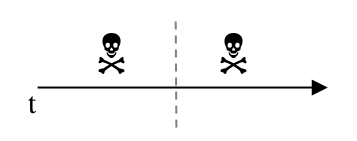
\includegraphics[scale=0.5]{figures/double-murder-knife-stabbing.png}
\captionof{figure}{Parts of a double murder event in a knife-stabbing scenario}\label{fig:parts-of-a-double-murder-event-in-a-knife-stabbing-scenario}
\end{figure}

Nonetheless, one could object that such an approach cannot account for situations such as a bomb scenario in which an intended explosion affected two victims leading to a double homicide. In such a case, quantification over temporally subsequent subevents is not possible since the explosion had an immediate effect and there was virtually no running time of the event. However, I believe there is no reason to assume that temporal chunks are the only possible parts that can constitute an event. Since events are complex peculiarities involving not only times, but also locations, in a bomb scenario described above it is still possible to differentiate between parts of an event in spatial terms. Consider the situation depicted in \figref{fig:parts-of-a-double-murder-event-in-a-bomb-scenario}. 

\begin{figure}[h!]
\centering
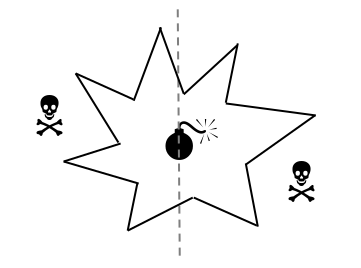
\includegraphics[scale=0.5]{figures/double-murder-bomb.png}
\captionof{figure}{Parts of a double murder event in a bomb scenario}\label{fig:parts-of-a-double-murder-event-in-a-bomb-scenario}
\end{figure}

Even with no temporally defined subevents it is quite straightforward that one could specify two areas within the space in which the explosion took place, as indicated by the dashed line. As a result, we obtain two parts of the murdering event each of which turns out to have the property of the whole and since individuals are in general assumed to occupy space, it should be possible to draw divisions like that with respect to any event.

Another way of explaining scenarios such as the one depicted in \figref{fig:parts-of-a-double-murder-event-in-a-bomb-scenario} would be to assume the uniqueness of roles condition on the individuation of events \citep[see][]{parsons1990events}. In such a case, the bomb explosion event can be described as consisting of two murdering subevents by distributing to different victims.

All things considered, it seems that the way of thinking about the meaning of multipliers I argue for can be easily extended to phrases involving reference to abstract peculiarities such as eventualities. Adopting a typal distinction between entities and events as typically assumed in standard Neo-Davidsonian frameworks \citep[e.g.,][]{carlson1984thematic,dowty1989semantic,parsons1990events}, along with the proposal that pluralities of events are obtained similarly to pluralities of entities \citep{bach1986algebra}, would simply require to ensure that the semantics of multipliers is general enough to cover both types of objects. In the next section, I will inspect yet another type of expression that is often modified by multipliers and does not necessarily denote concrete things. 

\subsection{Social roles}\label{sec:social-roles}

The final piece of data that appears to be problematic for the claim that multipliers are in fact subatomic quantifiers is constituted by phrases with nouns referring to social roles in examples such as those in \ref{ex:double-agent-polish}. 

\ex. Polish (NCP)\label{ex:double-agent-polish}
\ag. podwójny agent\\
double\textsc{.sg.m} agent\textsc{.m}\\
`double agent'\label{ex:double-agent-polish-agent}
\bg. podwójny mistrz\\
double\textsc{.sg.m} master\textsc{.m}\\
`double champion'\label{ex:double-agent-polish-champion}

Under ordinary circumstances, the phrase in \ref{ex:double-agent-polish-agent} does not refer to an individual who consists of two parts, e.g., Siamese twins working as spies, but rather they seem to involve a relationship between an individual and two other entities. To be an agent means to be an agent for some intelligence agency, i.e., one cannot be an agent without an employer for whom they spy. Likewise, \ref{ex:double-agent-polish-champion} refers to one person who is a champion in two disciplines. In both cases, the multiplier seems to quantify over entities denoted by the argument of the noun which at first blush is not expected given the previously discussed semantic behavior.

At this stage, it is not entirely clear how to integrate the ideas developed in this chapter with the treatment of examples such as those in \ref{ex:double-agent-polish}. However, a possible extension of the proposed view is to assume that nouns such as \textit{agent} involve some kind of an abstract association to entities related to denoted individuals, e.g., an association between agents and intelligence agencies, and that such an association is subject to part-whole relations. A promising perspective to pursue involves adopting the notion of roles into semantic theory \citep[see][]{sowa1984conceptual,steimann2000representation,zobel2017sensitivity,wagiel-toappear-slavic}. Intuitively, roles are functions or capacities of individuals, i.e., social constructs independent of the individuals that bear them. Crucially for our purposes, for an individual to bear a particular role, it must stand in a certain relationship to other individuals. Following \citet{zobel2017sensitivity}, one could distinguish between class nouns such as \textit{man}, i.e., properties of individuals of type $\langle e,t\rangle$, and role nouns such as \textit{agent} by adding a new type $r$ referring to roles and a shifting mechanism relating roles and individuals. Role nouns would then essentially denote properties of roles at type $\langle r,t\rangle$, but they could be shifted to refer to properties of entities as well. Within this view, multipliers would quantify over essential parts of roles rather than individuals and the whole phrase could then be shifted to refer to entities if required. This would account for the fact that expressions such as those in \ref{ex:double-agent-polish} denote individuals performing a complex role, i.e., individuals involved in activities and bearing responsibilities related to two distinct intelligence agencies. However, exploring the interaction between subatomic quantification and roles is rather challenging and goes beyond the scope of this study. Instead, in the next section I will return to the relationship between multipliers and cardinals.

\section{Multipliers vs. cardinals}\label{sec:multipliers-vs-cardinals}

As we saw in \sectref{sec:morphological-complexity-of-slavic-multipliers}, Slavic multipliers display morphological complexity, which suggests semantic compositionality. For instance, the Polish multiplier \textit{podwójny} `double' consists of the numeral root $\sqrt{\textit{dw}}$ corresponding to the number 2 present also in other types of numerical expressions, e.g., the cardinal \textit{dwa} `two', as well as additional morphemes including a special multiplicative circumfix \textit{po}$\rangle\dots\langle$\textit{n-}. This fact indicates that what multipliers and cardinals have in common is some sort of reference to integers. Though they both indicate that the number of quantified things equals 2, they differ in that they are devised to count entities of a distinct type. In particular, cardinals are semantically dedicated to count wholes. It is true that in Chapter \ref{ch:partitives-and-part-whole-structures} and \ref{ch:exploring-topological-sensitivity} we saw that they can be used in count explicit partitives in order to quantify over parts of objects, but notice that it is only possible when they modify a partitive word. In such a case, entities denoted by the whole partitive are treated as objects in their own right. Hence, the source of subatomic quantification is in fact the partitive, and the cardinal simply counts provided entities in their relative entirety. Bare cardinals can never access elements within a part-whole structure of a given entity. Rather, they always count entire objects in the denotation of a modified noun. On the other hand, multipliers are essentially subatomic quantifiers. They count parts of objects referred to by a modified nominal.

To better illustrate the claim introduced above, let us closely consider the contrasts between the truth conditions of the sentences involving numerical expressions in \ref{ex:cardinals-multipliers-crown-vault}. 

\ex. English (Guy Tabachnick, p.c.)\label{ex:cardinals-multipliers-crown-vault}
\a. There are two crowns in the vault.\label{ex:two-crown-vault}
\b. There are two parts of the crown in the vault.\label{ex:two-parts-crown-vault}
\b. There is a double crown in the vault.\label{ex:double-crown-vault}
\b. There are three double crowns in the vault.\label{two-double-crowns-crown-vault}

Under normal circumstances, there is no way the statement in \ref{ex:two-crown-vault} could be judged true if there were only two parts of a crown or crowns, e.g., an orb and a jewel, in the vault. The numeral phrase simply cannot be understood as referring to two parts instead of two entire objects.\footnote{Of course, what portion of an entity counts as an entire object is rather vague and might differ with respect to a particular predicate and a particular context. However, this is not at issue here.} In other words, cardinals are semantically devised to counting wholes. This is not in contradiction with the fact that in a sentence including a count explicit partitive construction as in \ref{ex:two-parts-crown-vault} the cardinal does count parts of a whole object. Consequently, \ref{ex:two-parts-crown-vault} would be true if there were only, say, an orb and a cross in the vault. Notice, however, that it is the partitive word that employs subatomic quantification. The cardinal here simply counts parts provided by the partitive construction as if they were considered objects in their own right. In other words, it does not operate on the part-whole structure of a given part. This contrasts with the meaning of \ref{ex:double-crown-vault} which would be true in a scenario where there were just one object in the vault. Crucially, however, that object would have to have two essential parts or, to put it differently, two parts having a property of being sort of a crown. Finally, the felicity of the sentence in \ref{two-double-crowns-crown-vault} shows that both types of quantification can co-occur within one phrase. Here, the multiplier triggers subatomic quantification constrained as discussed above, whereas the cardinal quantifies over wholes having the inner structure imposed by the multiplier. Consequently, the sentence would be true in a situation where in the vault there were three crowns such that each of them consisted of two self-sufficient parts. Notice that the relative order of the cardinal and multiplier as well as adjectival properties of the latter further suggest that subatomic quantification takes place first and only after the resulting wholes are counted.

The discussed contrast between cardinals and multipliers becomes even more salient if we consider what happens when the latter modify partitive words. Compare the examples in \ref{ex:two-double-part-adapter}. 

\ex. Polish\label{ex:two-double-part-adapter}
\ag. dwie części adaptera\\
two parts adapter\textsc{.gen}\\
`two parts of the adapter'\label{ex:two-part-adapter}
\bg. podwójna część adaptera\\
double part adapter\textsc{.gen}\\
`double part of the adapter'\label{ex:double-part-adapter}

We have already examined in detail count explicit partitives such as \ref{ex:two-part-adapter}, but let us now contemplate the meaning of an equivalent multiplier phrase such as \ref{ex:double-part-adapter}. Crucially, the multiplier quantifies over parts of a part of the adapter. The whole expression would be true of an entity that is an adapter part and consists of two comparable parts. Yet again, the multiplier employs quantification within the part-whole structure of a thing denoted by the nominal no matter what that thing is. Though such a use is for sure very rare, the phrase is definitely interpretable.\footnote{The example was actually found on a website of a producer of adapters with a picture of a described part. Source (accessed on 10th November 2020): \url{https://www.kstools.com/pl/produkty/narzedzia-specjalistyczne-do-samochodow-osobowych/silnik-system-paliwowy/czesci-pojedyncze/2159/podwojna-czesc-adaptera}.}

A natural example of a sentence with the discussed construction attested in the NCP is provided in \ref{ex:double-part-wall}.

\ex. Polish (NCP)\label{ex:double-part-wall}
\bg.[] Skrzynkę horyzontalną otwiera się podobnie jak podwójną część przedniej ścianki [\dots]\\
box\textsc{.acc} horizontal\textsc{.acc} opens \textsc{refl} similar how double\textsc{.acc} part\textsc{.acc} front\textsc{.gen} wall\textsc{.gen}\\
`The horizontal box can be opened similar to the double part of the front wall [\dots]'

I conclude that the purpose of cardinals is essentially to count whole entities in the extension of a modified nominal. If they modify a regular noun, they simply quantify over objects in its denotation. Similarly, if they appear in a count explicit partitive, they count provided parts in their entirety as if they were wholes. At the same time, natural language developed a special type of expression dedicated to numerical subatomic quantification, namely multipliers. Multipliers differ from cardinals in that they always count essential parts of objects denoted by a modified nominal be it a whole or a part. In other words, they are equipped to count parts within a whole. On the other hand, the two categories are similar in that although they typically count, sometimes they seem to measure. The quantificational properties of the two numerical expressions in question are summarized in  \tabref{tab:properties-of-cardinals-and-multipliers}.

    \begin{table}[h]
    \centering
\begin{tabular}{lcc}
\lsptoprule
                           & \textsc{cardinals} & \textsc{multipliers}  \\ \midrule
subatomic quantification   & *               & $\checked$    \\
quantification over wholes & $\checked$               & *    \\ \lspbottomrule
\end{tabular}
\caption{Properties of cardinals and multipliers}
\label{tab:properties-of-cardinals-and-multipliers}
\end{table}

This concludes the examination of some non-trivial properties of the neglected class of multipliers with respect to the issues concerning subatomic quantification. 

\section{Summary}\label{sec:summary-ch4}

In this chapter, I focused on a key topic concerning subatomic quantification. Specifically, I presented novel evidence demonstrating that in natural language there are numerical expressions devised for the purpose of quantification over parts, namely multipliers such as English \textit{double}. The fact that such lexical items are cross-linguistically widespread indicates the relevance of part-whole structures of singular objects for the interaction between parthood and quantification in natural language semantics. The morphological evidence from Slavic demonstrates that Polish, Czech, Russian, and Bosnian-Croatian-Serbian multipliers are formally complex expressions derived from numeral roots of corresponding cardinals. I argued that the morphological complexity of Slavic multipliers suggests semantic compositionality. 

Multipliers are sensitive to the internal part-whole structure of objects denoted by nouns they modify and involve quantification over cognitively most salient elements of those objects. Often, such elements are self-sufficient parts, i.e., entities that have a property comparable with the property of the whole. Sometimes, they are not self-sufficient but rather they are considered the most significant parts within the inner structure of an object. I generalized that multipliers count essential parts, i.e., parts perceived as crucial for an entity to be considered as having a particular property, with self-sufficient parts constituting a subset thereof. Moreover, I examined multiplier phrases involving mass terms. Interestingly, such expressions receive a portion interpretation and as such are countable. This fact indicates that multipliers either perform or require a mass-count shift in terms of packaging. Furthermore, I proposed how the view argued for here could be extended to cover cases of multiplier phrases involving other types of NPs, namely event nominals and role nouns. Incorporating abstract objects such as eventualities and roles into the ontology would allow us to capture the meaning of virtually all multiplier phrases in terms of one unified mechanism. Finally, I discussed how multipliers differ from cardinals. The crucial distinction between the two boils down to what type of entity they count in terms of part-whole structure. In particular, while cardinals always quantify over wholes, multipliers always count parts of a singular object which, similarly to complex entities or events they constitute, have themselves a property considered essential for an entity to fall in the denotation of a modified noun. 

This chapter concludes the empirical part of this book. The most important insights could be summarized as follows. First, singulars and plurals share a unified part-whole structure. Second, natural language is sensitive to topological relations holding between parts of entities in the denotations of nominal expressions and allows for quantification at the subatomic level. Third, only entities that are perceived as constituting integrated wholes are conceptualized as countable. Finally, though different types of numerical expressions specialize in quantification either over wholes or over parts, the underlying mechanism is the same. In the next chapter, I will introduce the conceptual background that will serve as an informal notional basis for a formal account for subatomic quantification.

\chapter{Conceptual background}\label{ch:conceptual-background}

In the previous three chapters, I discussed novel data concerning the interaction between partitivity and countability. In particular, I presented linguistic evidence suggesting that singulars and plurals do not differ with respect to the part-whole relation they employ but rather that parts of singularities remain in a particular topological configuration ensuring that the whole constitutes an integrated object, whereas parts of pluralities do not, and thus form a scattered entity. This claim is motivated by two linguistic facts. First, cross-linguistically the same partitive words can appear both in entity and set partitives. Second, the contrast between regular plurals  and Italian irregular plurals reveals a crucial topological distinction between the two. Furthermore, I showed that natural language does not allow for counting arbitrary sums of topologically unrelated parts. Only entities that are conceptualized as constituting continuous objects can be subject to counting. This restriction appears to hold both on the level of wholes and on the subatomic level, as the evidence concerning topology-sensitive partitive words as well as the semantic behavior of multipliers indicate. In other words, quantification in natural language is sensitive to topological relations between parts of entities it operates on.  

In this chapter, I will discuss the conceptual background concerning countability and subatomic quantification I assume here. In particular I will present three claims regarding the relevance of topological notions in nominal semantics, general counting principles, and their significance for subatomic quantification. This informal conceptual framework will motivate the formal account for the core phenomena explored in this study, which I will develop in Chapters \ref{ch:theory-of-parts-and-wholes} and \ref{ch:mereotopological-account-for-subatomic-quantification}. However, before I present in detail the notional core of this study, let us cgonsider a more general cognitive context. Though the linguistic evidence presented so far is compelling and entirely motivates the claims, I believe it is useful to confront it with what we know from psychological research in order to provide supplementary support. 

\section{Psychological evidence}\label{sec:psychological-evidence}

In this section, I will review psychological evidence that demonstrates several factors concerning human cognition that correlate with the linguistic evidence introduced in Chapters \ref{ch:partitives-and-part-whole-structures}, \ref{ch:exploring-topological-sensitivity}, and \ref{ch:multipliers}. First, I will discuss the relevance of how spatial categories such as solidity, shape, and most importantly integrity of entities are conceptualized with respect to the mass/count distinction in grammar. Furthermore, I will consider the significance of the part/whole distinction for language acquisition and review the evidence that humans have simultaneous perception of an object as a whole and as a collection of parts. Finally, I will discuss what cognitive studies tell us on number sense in humans, especially on the relation between integrity and counting in young children. The literature on each topic is abundant. For the sake of brevity, in each case I will only refer to a few representative studies.

\subsection{Object/substance distinction}\label{sec:object-substance-distinction}

I will start with a brief overview of the research in cognitive psychology relating individuation with the difference in perception of solid objects and amorphous substances, which suggests that this distinction is relevant to the phenomenon of countability in natural language. In the past 30 years, convincing evidence has been presented that indicates that the distinction between objects and substances is not merely an alternation based on grammar. Contrary to \citeposst{quine1960word} influential claim that it is language what provides the means for individuation of objects \citep[see also][]{pelletier_schubert1989mass}, it appears that count and mass syntax reflect on how we see entities in the world rather than the other way round. In other words, the research to be discussed here shows that the distinction between objects and substances is not something conventional, formal, or arbitrary imposed by the way a particular language is devised, i.e., a way of speaking so to say. To the contrary, it appears to be a deeply embedded component of human cognition manifesting itself in non-verbal infants at a few months of age and shared with non-human species. 

Multiple experiments demonstrate that children associate count nouns with solid discrete objects at an early age \citep[see, e.g.,][]{landau_smith_jones1988importance,soja_carey_spelke1991ontological,imai_gentner1997crosslinguistic}. The evidence comes from the results of the so-called word extension task, which concerns learning new words by subjects. The procedure is as follows. First, a child is presented with a novel entity and instructed on what it is called. That entity can be either a solid object or a shapeless portion of a substance. Next, two other entities resembling the initial one with respect to different perceptual features are introduced. One would match the already introduced entity in shape, whereas the other would be of the same material. Interestingly, extensive research shows that children extend the name of a novel item to items of the same shape only if the initial entity was a solid discrete object. On the other hand, if they were first presented an amorphous portion of a novel substance, they do not extend its name to items of a similar shape, but rather to objects made out of the same material.

Based on such evidence, \citet{soja_carey_spelke1991ontological} argue that certain ontological commitments are prior to the linguistic mass/count distinction, contrary to \citeauthor{quine1960word}'s claim. Additional support for such a conclusion comes from the fact that the results were replicated in populations using languages with syntax significantly different from English. For instance, \citet{imai_gentner1997crosslinguistic} demonstrate parallel evidence based on the same experimental paradigm using the word extension task in the Japanese speaking environment. Though Japanese lacks a straightforward morpho-syntactic equivalent of the distinction between mass and count nouns present in languages such as English, Japanese speaking children distinguish between objects and substances just as well as their English speaking peers.

A number of studies provide varied and carefully controlled evidence that preverbal children are endowed with certain assumptions concerning the nature of objects \citep[e.g.,][]{carey1985conceptual,spelke1990principles,soja_carey_spelke1991ontological,carey_spelke1996science}. For instance, they expect objects to be bounded and cohesive. The former assumption reflects on an entity having natural boundaries, whereas the latter translates into an anticipation that objects have parts that stick together. Furthermore, objects are expected to move across space as wholes along continuous paths and to retain identity upon collisions with other entities. On the other hand, substances lack any of those properties. An exemplary experimental paradigm is as follows. An infant is introduced either to a solid object, e.g., a teddy bear, or a portion of substance, e.g., clay, displayed in front of them. Next, the entity is covered by a screen and the child sees that a second item is placed behind the screen. Finally, depending on an experimental condition after the screen was removed either there were two items revealed or due to the manipulation by an experimenter only one item could be seen. Interestingly, if the initially introduced entity was a discrete solid object, children reacted with great surprise if after removing the screen they could find only one item. On the other hand, no such reaction was recorded if they were introduced to a portion of a substance at the beginning. The conclusion is that preverbal children appear to know the difference between objects, pluralities thereof, and substances. They expect that if one adds a teddy bear to a teddy bear, the result should be two teddy bears, whereas if one combines clay with clay, one does not get a plurality of clay. Since similar results were also found in non-human primates (see, e.g., \citealt{hauser_carey2003spontaneous,hauser_spaulding2006wild} on rhesus monkeys), it seems plausible to assume that this property of human cognition has some evolutionary history. I will come back to the issue of number in \sectref{sec:number-sense}.

However, though the difference between discrete solid objects and amorphous substances has a significant status in the cognitive and linguistic development of children, it turns out that the correlation between this distinction and mass/count syntax is imperfect. A corpus study on toddler vocabulary pursued by \citet{samuelson_smith1999early} shows a significant asymmetry between particular syntactic categories. Specifically, while the large majority of nouns that English speaking children learn early are count nouns (74\% of the vocabulary), only a small portion involves mass nouns (10\% of the vocabulary). There is also a third class of expressions that is considered ambiguous between count and mass (16\% of the vocabulary). The results of the examination in order to find out whether the object/substance distinction correlates with the mass/count distinction are somewhat surprising. In general, a correspondence between solid objects and count nouns, on the one hand, and non-solid entities, on the other, was in fact observed. However, it was imperfect and \citeauthor{samuelson_smith1999early} recognized a number of interesting mismatches. Surprisingly, while solidity and shape turn out to be good predictors of count nouns, mass nouns appear to be less correlated with non-solidity and shapelessness.\footnote{Notice that probably the main reason explaining this result is the existence of the category of object mass nouns such as \textit{furniture} and \textit{kitchenware}.}

Yet another strand of research provides support for the findings discussed above. In particular, \citet{prasada_ferenz_haskell2002conceiving} demonstrate that categorization of a noun as countable or uncountable does not reduce to establishing an immutable ontological distinction between an object and a substance. Rather, it seems that speakers of languages such as English categorize nouns in terms of countability based on whether they construe entities they refer to as objects or as substances. A series of experiments utilizing novel vocabulary tasks show that a novel item that has an irregular shape is less probable to be referred to by a novel count noun when contrasted with entities of a regular shape. However, the same item is significantly more probable to be considered countable when displayed among other similar entities having such an irregular shape. This means that it is not the case that some objective properties of things influence the way grammar is directly. Instead, the mass/count distinction appears to reflect how humans conceptualize entities in the world.

To conclude, the psychological research reviewed in this section indicates that contrary to \citeauthor{quine1960word}'s claim, human beings apparently do have certain ontological commitments prior to acquiring the syntax of a particular language. Specifically, the way children are biased towards perceiving objects as opposed to substances correlates with the mass/count distinction in grammar. However, this correspondence is not of a one-to-one  type and there are well-known cases of mismatches. Yet, it is crucial that the distinction in grammar is not due to different ontological categories in some objective sense, but rather it reflects on how entities in the world are conceptualized. In the next section, I will discuss the relevance of part-whole structures in the process of language acquisition. In particular, I will briefly review how a certain bias concerning what it means to be a whole guides children in how they learn lexical meanings of nouns. 

\subsection{Whole object assumption}\label{sec:whole-object-assumption}

Since at least the early 1990's, language acquisition studies have shown that vocabulary development is constrained by certain mechanisms that govern it in order to ensure its effectiveness. In particular, children are guided by a number of word learning biases i.e., endowed assumptions that allow us to eliminate unlikely alternatives in order to efficiently process and learn new lexical meanings \citep[see, e.g.,][]{markman1990constraints,hollich_golinkoff_hirsh-pasek2007young,hansen_markman2009children}. Such assumptions begin to manifest around the age of 18 months when rapid expansion of a child's vocabulary starts. They are crucial in deciding what the reference of a new noun is, e.g., what aspect of an object it designates, as well as in solving the problem of indeterminacy. One of the word learning biases that will be of special interest to us here is the so-called whole object assumption \citep{markman1990constraints}. 

The whole object assumption allows children to constrain the meaning of novel words by guaranteeing that a child relates a new noun with an object in its entirety rather than with some arbitrary part or property of that object \citep{markman1990constraints}. For instance, if an adult points to an item and labels it, e.g., by uttering \textit{a doll}, a child assumes that the noun \textit{doll} is meant to refer to the whole object and not to its part or its certain characteristic. Though in principle the adult's verbal behavior might have been interpreted as referring to the doll's head, leg, dress, color, or size, children intuitively rule out such possibilities and associate the label with the whole item.\footnote{See \citet{quine1960word} for a related problem of the inscrutability of reference.} This bias holds even in situations where an object's color or a certain dynamic activity are made salient to a child \citep{hansen_markman2009children}.

Though the original research regarded 18-month-year old children and older, later studies have demonstrated that in fact infants can associate nouns with whole objects already at the age of 12 months \citep{hollich_golinkoff_hirsh-pasek2007young}. Crucially, the effect was attested despite the fact that test items could be viewed as two separate objects and even when a certain part of an item was made salient. Interestingly, similar results were obtained in experiments where participants were adult. Hence, the mechanism appears to be deeply embedded. Its relevance lies in that it enables children to determine which of the numerous logically possible meanings a word could have is actually the correct one.

In this section, we saw that children distinguish intuitively between parts and wholes. In the process of language acquisition, when exposed to a novel noun, they do not attribute its meaning to a part of an object it refers to but rather immediately assume it is true of a whole thing. The whole object assumption has often been related to the findings concerning infants' perception of objects discussed in the previous section. It has been hypothesized that the constraint in question reflects the non-linguistic status of objects \citep{hollich_golinkoff_hirsh-pasek2007young}. This might suggest that from the perspective of a child the fact that wholes involve parts is somewhat discriminated. However, the evidence is much more complex. In the next section, I will provide a brief overview of the study of part-whole perception in children.

\subsection{Part-whole perception}\label{sec:part-whole-perception}

It is a cognitive fact that we often conceive of entities as being made up of smaller entities related to each other in a particular manner. Experimental evidence shows that humans have two simultaneous perceptions concerning part-whole structures of entities \citep[e.g.,][]{witkin1950individual,meili-dworetzki1956development}. On the one hand, we possess the ability to discriminate parts from a whole, i.e., decompose an entire object into distinct elements making it up. On the other hand, we are able to integrate the total sum of the parts into a complete whole. This phenomenon is usually referred to as part-whole perception and it is standardly attributed to the ability of an individual to decenter, i.e., to shift attention from parts to the whole or vice versa \citep[see][]{piaget_morf1958isomorphismes}.

Though adults in general show part-whole perception, it has been subject to controversy in the psychological literature at what age it emerges. In the early Piagetian studies, the experimental results suggested that this ability is absent in young children \citep{elkind_koegler_go1964studies}. In a typical experiment, a child was presented a drawing of a whole consisting of parts that were independent objects in their own right, e.g., a person made out of fruits as in \figref{fig:part-whole-perception}, and was instructed verbally to report what they see. 

\begin{figure}[h!]
\centering

\includegraphics[scale=0.3]{figures/fruitman.png}
\captionof{figure}{Part-whole perception \citep{elkind_koegler_go1964studies}}\label{fig:part-whole-perception}
\end{figure}

According to \citeauthor{elkind_koegler_go1964studies}, children report that they perceive simultaneously a whole and parts attributed to the same form, e.g. both a man and fruits, only at the age of 8. Before that age, subjects failed in complete decentration with 5-to-6-year-olds showing complete centration, i.e., they reported that they saw only parts, e.g., fruits but not a person, and older children gradually improved. However, later studies suggest that part-whole perception develops much earlier. For instance, \citet{kimchi1993basic} provides evidence that 5-year-old children show sensitivity to parts and to part-whole relations and that this sensitivity improves with age. Even more interestingly, \citet{boisvert_standing_moller1999successful} show that 3-year-olds demonstrate good performance in part-whole perception tasks using multiple-choice tests instead of Piagetian verbal tasks used in earlier studies. Finally, \citeposst{quinn_burke_rush1993part} results indicate that 3-month-old infants can group elements of visual pattern information into larger perceptual units based on lightness similarity in a way that suggests at least some component of part-whole perception.

I interpret the experimental results presented above as suggesting that human cognition is devised to be sensitive to part-whole structures since even very young individuals can decompose a whole into pieces by discriminating its parts as well as represent individual elements as making up an integrated collection that is a whole. Since these two perceptions are simultaneous, one could expect that we intuitively categorize entities as certain configurations of smaller things that despite their often complex inner structure are singular objects. At the same time, parts of such objects remain cognitively salient and if required, can be easily accessed. If the conclusions from the experiments reported above are on the right track, this property of the human mind appears to be either innate or at least to emerge at an early stage of cognitive development.

\subsection{Number sense}\label{sec:number-sense}

The final piece of cognitive evidence to be discussed here concerns human number sense, i.e., an intuitive understanding of what numbers mean and how they can be affected by various operations (see, e.g., \citealt{dehaene1997number} for an overview). This mental mechanism allows for a special type of sensory perception through which the cardinality of a given set of entities can be perceived with similar ease as their size, color, shape, or position and as such provides the basis for various forms of calculation. In humans, number sense is based on two different cognitive systems, specifically the approximate number system (ANS) and the object tracking system (OTS) \citep[see, e.g.,][]{hyde2011two}. The ANS is a cognitive system supporting the imprecise estimation of the numerical magnitude of a collection of objects without relying on symbolic representations (see, e.g., \citealt{feigenson_et-al2004core,nieder_dehaene2009representation} for an overview). It manifests already in infants and gets more developed with age \citep{cantlon_et-al2006functional}. In contrast, the OTS is the mental ability to independently track up to 4 entities without counting by means of parallel individuation (see, e.g., \citealt{carey1998knowledge,carey2009origin} for an overview). Though the acquisition of abstract number concepts, even for low numbers, appears to require more than only the ANS and the OTS, both capacities seem to support this process (e.g., \citealt{hyde2011two}; but see \citealt{piazza2010neurocognitive} for arguments for the crucial role of the ANS rather than the OTS).

It appears that there is evidence indicating that humans are at least to some extent predisposed to develop certain numerical abilities such as the concept of exact number and simple arithmetic based on their number sense. For instance, \citet{gelman_gallistel1978child} argue that children are endowed with innate principles of counting and have intuitive understanding of the cardinality of a set of entities and its conservation under changes that do not affect quantity. It seems that a lot of knowledge concerning how to put objects in a one-to-one correspondence with numbers is intuitively understood by children though it is never taught or formulated in an explicit way. In particular, when learning to count children are not taught that each entity must be counted once and only once, or that one number cannot be associated with more than one entity, but this principle is taken for granted. Moreover, children know intuitively that number words are supposed to be recited in a fixed order and that the last numeral represents the cardinality of the whole enumerated set. According to this view, innate knowledge regarding counting principles precedes and facilitates the acquisition of that part of the lexicon that includes number words and guides its application in a particular situation of counting.\footnote{However, see \citet{fuson1988springer} for an opposing view claiming that children learn counting by imitation. For instance, \citeauthor{fuson1988springer} argues that children recite strings such as \textit{onetwothreefourfive}\dots {} as uninterrupted sequences and only later on they segment them in order to delimitate numerals, learn to extend them to larger values and to apply them to particular situations.}

The above introduced hypothesis seems to be corroborated by further experimental evidence that suggests that at the age of 2.5 years children understand that counting is an abstract procedure that can be applied to different kinds of objects including concrete entities as well as events \citep{wynn1990children}. 3.5-year-olds know that the order in which they recite numerals is crucial, whereas the order of pointing at counted items is irrelevant as long as each item is counted and no one item is counted twice. Furthermore, children are able to indicate and correct subtle errors that result from violations of basic counting principles such as reciting numerals out of order, counting the same object twice, or omitting an item while counting \citep{gelman_meck1983preschoolers,gelman_meck_merkin1986young}. By the age of 4 years, children show that they have already mastered the basics of counting and that they can generalize the procedure to novel situations. Older children often spontaneously reinvent arithmetic developing new strategies for calculating that best fit for a particular problem \citep[p. 119]{dehaene1997number}.

However, probably the most intriguing finding from the perspective of the interest of this study is a tight link between spatial integrity and numerical information observed in young children. Specifically, \citet{shipley_shepperson1990countable} provide a particularly striking demonstration of the relevance of objects understood as integrated discrete physical entities for the cognition of 3-to-4-year-olds. In the experiment, children were presented sets of items and instructed specifically what they were supposed to count. For instance, an array of forks with one item broken in two pieces as illustrated in  \figref{fig:relevance-of-integrity-in-counting} was displayed in front of a child who was then asked to count the forks. 

\begin{figure}[h!]
\centering
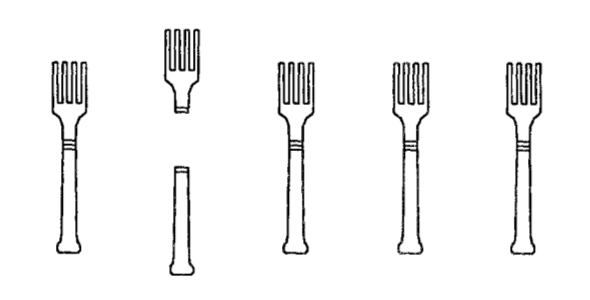
\includegraphics[scale=0.4]{figures/forks.png}
\captionof{figure}{Relevance of integrity in counting (\citealt[p. 60]{dehaene1997number}; adapted from \citealt{shipley_shepperson1990countable})}\label{fig:relevance-of-integrity-in-counting}
\end{figure}

Unlike adults and older children, children between 3 and 4 years of age did not answer that there are five forks, but rather that there six of them, i.e., they counted each detached part of a fork as a separate entity. Similarly, when instructed to count kinds, e.g., different kinds of animals, or properties, e.g. different colors, in a setup where each kind or property was exemplified by a number of distinct discrete items, children included each separate object in their count.

The results demonstrate that the canonical countable entity for a young child is a discrete physical object that comes in a single piece. The role of spatial integrity is crucial in determining what counts as one and this bias precedes the process of learning how to count. In other words, at an early stage of development of arithmetic abilities young children simply cannot avoid counting each discrete integral object as one unit. It is very likely that the assumption that number is a property of sets consisting of discrete spatially contiguous objects is a deeply embedded principle that facilitates mastery of counting.\largerpage[2]

The findings of \citeauthor{shipley_shepperson1990countable} were further confirmed for other forms of linguistic quantification in experiments based on quantity judgment tasks involving comparative constructions and pluralization \citep{melgoza_pogue_barner2008broken}. In particular, when presented an object divided into three parts, e.g., a broken fork, on the one hand, and two whole objects, e.g., two integral forks, on the other, 4-year-old children judged the former to be more objects than the latter. Furthermore, in an elicitation task children often labeled broken objects using plural morphology. For instance, a phrase \textit{some forks} was used to refer to three separated pieces of a broken fork. The results presented by \citeauthor{melgoza_pogue_barner2008broken} not only confirm the findings of \citeauthor{shipley_shepperson1990countable} but also indicate the existence of a spatial bias for many forms of quantification in natural language. In all tested cases, the spatial criterion of integrity was preferred over other factors in order to establish what counts as one. In other words, when children quantify sets, they seem to define individual set members in terms of spatial contiguity in the first place. I take these results to be  evidence suggesting that countability as a property of sets of discrete separate entities is a deeply embedded principle. Though as we know from every-day life experience adults can develop a mechanism to retrieve the original part-whole structure of counted entities, e.g., reconstruct a whole fork by combining separate pieces in thought, I hypothesize that the underlying quantificational procedure is based on a principle relating numbers with things that are conceptualized as coming in one piece.{\interfootnotelinepenalty=10000\footnote{Admittedly, one can also count concrete entities such as functional units that do not seem to be integrated in a topological sense. For instance, a pestle and mortar can count as a single piece of kitchenware \citep{sutton_filip2016counting}. Nevertheless, I argue that in such cases the notion of integrity still applies, though it is not physical integrity but rather functional units are conceptually integrated in the sense that they are united under some functional role \citep[see][]{grimm_levin2017artifacts}. I will come back to this issue in \sectref{sec:functional-units}.\label{fn:artifacts}}} However, before I conclude, I will briefly discuss how human quantification differs from number sense in other animals.

Massive evidence indicates that number sense is not exclusive to human mind. Well-established research in etiology shows that apprehension, comparison, and even approximate addition of quantities is also present in animals (see, e.g., \citealt[pp. 13--40]{davis_perusse1988numerical,gallistel1989animal,dehaene1997number} for overview). The most well-known evidence concerns the ability to represent and discriminate quantities of relative sizes in primates \citep[e.g.,][]{woodruff_premack1981primative,matsuzawa1985use,rumbaugh_et-al1987summation,washburn_rumbaugh1991ordinal,boysen_et-al1996quantity}, but it is also found in other mammals such as dolphins \citep{mitchell_et-al1985discriminative}, cats \citep{thompson_et-al1970number}, and rats \citep{capaldi_miller1988counting}, as well as birds \citep{pepperberg1987evidence} and even fish \citep{agrillo_et-al2012evidence}. Furthermore, recent studies in botanics suggest that there are reasons to also assume plant arithmetic \citep{bohm_et-al2016venus}. The evidence indicates either that number sense is an evolutionary ancient part of cognition or that there were multiple convergent evolution events. In any case, it is a widespread phenomenon shared by a wide range of species.

However, despite the large body of evidence indicating that many non-human animals have the approximate number system, their number sense seems to differ significantly from that of humans. Though there are well-documented cases of approximate quantification in animals, no case of symbolic addition is known in any species other than the chimpanzee, and there only after long training dedicated to learning a small set of digits and with frequent errors in computation \citep[p. 39]{dehaene1997number}. On the other hand, young children spontaneously count on their fingers, often up to 10 before the age of three and acquire the syntax of complex numerals with ease. Thus, the more lax concept of numerosity is often used with respect to animal quantification in order to distinguish it from the symbolic and verbal representation of number in humans. To conclude, though some forms of quantification appear to be frequent in the animal kingdom, they seem to differ significantly from what humans do when they count. While non-human animals estimate quantities on a regular basis, it seems that the ability to establish a one-to-one correspondence between an object and a discrete symbol which allows for computation of the exact number of entities in a given set is an extremely rare property among species. 

It seems that counting as performed by humans is a quite unique ability which associates discrete entities with abstract representations of number. I hypothesize that the core  mechanism underlying all counting manifests in early childhood and concerns establishing a one-to-one correspondence between integral physical objects that come in one piece and integers. In other words, I assume that the topological notion of spatial integrity is the basis for what counts as one, and only later humans develop ways of abstracting away from this principle, e.g., by extending it to quantification over abstract entities such as kinds and properties, or by being able to retrieve the original connection between detached parts. In the following sections, I will attempt to relate the linguistic evidence presented in Chapters \ref{ch:partitives-and-part-whole-structures}, \ref{ch:exploring-topological-sensitivity}, and \ref{ch:multipliers} with the conclusions of cognitive psychology in order to develop the three main claims of this study that will serve as a conceptual background for the formal account for subatomic quantification in natural language, to be developed in Chapters \ref{ch:theory-of-parts-and-wholes} and \ref{ch:mereotopological-account-for-subatomic-quantification}.

\section{The three claims}\label{sec:the-three-claims}

I have already presented a broad range of data demonstrating both the relevance of subatomic structures in natural language and the important role that the way entities including parts of a whole are spatially related to each other plays with respect to quantification. Furthermore, in the previous section I reviewed additional psychological evidence suggesting that these issues are deeply embedded in human cognition. Now is the time to discuss in detail what I believe to be the conceptual core of this study, namely the three claims I make with respect to the interaction between parthood, topology, and quantification in natural language. I will start with postulating that natural language semantics is sensitive to topological relations holding between elements within part-whole structures designated by nominal expressions. Next, I will posit a set of general counting principles, including constraints concerning non-overlap, maximality, and integrity of counted things. Finally, I will postulate that the very same universal mechanism applies irrespective of whether one quantifies over entire entities or over parts of a whole.

\subsection{Relevance of topological notions with respect to part-whole structures}\label{sec:relevance-of-topological-notions-with-respect-to-part-whole-structures}

It is well-known that topological notions play an important role in natural language. The existence of locative expressions involving prepositions such as \textit{inside}, \textit{near}, \textit{under}, \textit{between}, and \textit{far} shows that relations concerning how we conceptualize position and space are deeply rooted in grammar. Arguably, they constitute universal components of human cognition and natural language semantics. Though the research on locative PPs is well-established and contributed to our understanding what means language uses to encode information regarding location of objects with respect to each other \citep[e.g.,][]{clark1973space,herskovits1985semantics,zwarts_winter1997semantic,kracht2002semantics}, the question concerning spatial constitution of entities remained somewhat elusive in the study of meaning. One line of argumentation justifying why those kinds of issues should remain unaddressed is that they simply stem from every-day world knowledge, and thus, as extra-linguistic factors, are not supposed to be incorporated into semantic theory. For instance, \citet{schwarzschild1996pluralities} famously argues that the fact that \ref{ex:bill-texas} entails \ref{ex:brain-texas} has nothing to do with referential properties of the subject DPs in both sentences. Rather, the inference simply results from facts concerning what we know about where brains are located. 

\ex. English \citep[p. 187]{schwarzschild1996pluralities}\label{ex:bill-brain-texas}
\a. Bill is in Texas.\label{ex:bill-texas}
\b. Bill's brain is in Texas.\label{ex:brain-texas}

\citeauthor{schwarzschild1996pluralities} might seem right for examples such as \ref{ex:bill-brain-texas}. However, in previous chapters of this study we saw that there are a number of natural language expressions that are sensitive to topological properties of part-whole structures corresponding to their referents. My view is that if we want to account for the meaning of nouns in its entire complexity, topology-related phenomena deserve serious consideration.

It has been acknowledged for a long time that nominal semantics differentiates between count singulars referring to integrated objects, on the one hand, and mass terms and plurals denoting scattered entities and arbitrary sums of individuals, respectively, on the other. As we saw in \sectref{sec:object-substance-distinction}, there are good reasons to assume that this contrast correlates with some fundamental properties of human cognition. Soon, we will see that the distinction can be captured in terms of how parts constituting a whole are spatially arranged. However, before I even start considering how to develop a proper account, it is crucial to realize that the extent to which topology plays a role in part-whole structures associated with referents of nominals is highly underestimated, if not neglected, in the contemporary mainstream research on pluralities and countability. One of the important empirical contributions of this study is about compensating this deficit. 

The data presented in Chapter \ref{ch:partitives-and-part-whole-structures} and \ref{ch:exploring-topological-sensitivity} show that certain classes of nouns encode certain types of spatial configurations of entities making up a whole. In particular, at least some Italian irregular plurals discussed in \sectref{sec:italian-irregular-plurals} denote integrated pluralities, i.e., sums of individuals that form cohesive wholes. On the other hand, different types of topology-sensitive partitive words explored in \sectref{sec:continuous-discontinuous-parts} and \sectref{sec:more-topology-sensitive-partitive-words} involve reference to continuous parts whereas extensions of their topology-neutral counterparts comprise also discontinuous portions of a whole. Though the evidence explored in this study emphasizes specifically the role of integrity in subatomic quantification, recent research on different types of collective nouns and mass terms points to a similar conclusion regarding the relevance of topology in nominal semantics on independent grounds. In particular, \citet{grimm2012number} proposes that a subset of mass nouns that denote aggregates of granular objects, hence granular mass terms like \textit{rice} and \textit{gravel}, involve reference to clustered individuals, i.e., bundled entities transitively connected to each other. In a similar vein, \citet{henderson2017swarms} argues that swarm nouns such as \textit{grove}, \textit{horde}, and \textit{swarm} denote large pluralities whose constituents remain in proximity within a certain spatial configuration. Moreover, \citet{grimm_docekal-toappear-counting} and \citet{wagiel-toappear-slavic} discuss a particular class of Slavic derived mass nouns, such as Czech \textit{list} `leaf' $\sim$ \textit{listí} `foliage', that refer to collections of singular entities that are easily distinguishable yet conceptualized as aggregates.\footnote{For experimental investigation into the meaning of such expressions in Czech and Polish, see \citet{docekal_wagiel2018decomposing}.} Finally, as proposed by \citet{grimm2012number}, referents of concrete count nouns can be viewed as entities whose part-whole structure is constrained in such a way that it forms an integrated object in its own right.

The psychological evidence discussed in \sectref{sec:psychological-evidence} emphasizes the role of spatial integrity of objects, on the one hand, and our ability to simultaneously perceive individual parts of such cohesive wholes as entities in their own right, on the other. Given the amount of linguistic evidence supplemented with findings concerning human cognition, I argue that semantic theory needs to accommodate those facts. In other words, my first claim is as follows. There is more to the meaning of common nouns than usually assumed, and without a proper approach incorporating the insights concerning the role of topological notions in part-whole structures many phenomena will be left unexplained or even unnoticed. I posit that a good starting point is to try to capture the difference between count singulars, regular plurals, and mass nouns in terms of different topological relations encoded within corresponding part-whole structures. Specifically, count singulars refer to entities that constitute integrated wholes whose parts stick together, rather than mere collections of spatially unrelated portions of matter. On the other hand, plural nouns denote arbitrary sums of such individuals, i.e., they require their parts to be constrained by spatial integrity but impose no topological restrictions on configurations in which they appear. Finally, a proper treatment of mass terms should account for the fact that their prototypical referents are scattered unbounded entities. An additional advantage of such a novel perspective is that it suggests that different part-whole structures do not emerge due to distinct parthood relations. Instead, it seems that different part-whole structures arise as a result of the interaction between one unified parthood relation with distinct topological notions. In the next section, I will posit that the postulated view on what it means to be a whole can shed new light on countability.

\subsection{General counting principles}\label{sec:general-counting-principles}

In general, I follow a well-established linguistic tradition assuming that the mass\slash count distinction corresponds to a contrast concerning how different types of entities are conceptualized \citep[e.g.,][]{wierzbicka1988semantics,chierchia1998plurality,chierchia1998reference,chierchia2010mass,chierchia2015universal,grimm2012number}. As we saw in \sectref{sec:psychological-evidence}, a substantive body of research in cognitive psychology provides evidence that human beings categorize stable bounded things that preserve shape differently than amorphous substances. The former are considered delimited objects whose spatial identity can be tracked easily throughout time, whereas the latter are perceived merely as unindividuated portions of matter. On the other hand, there appears to be rich intuitive knowledge concerning what counting is, which seems to be part of human cognitive endowment. The exact nature of how cognitive facts relate to natural language semantics and grammar, i.e., the structure and meaning of certain syntactic constructions,  might not be straightforward. Therefore, the view that I propose here is most probably a simplified account. Nevertheless, I believe that it reveals what I argue is an advantageous perspective on what it means to be countable. 

Usually in the study of countability, at some point when it comes to defining what counting is something like `counting is quantification over what counts as one' is stated. Often, `what counts as one' is understood in terms of atomicity. In particular, an atom in a technical sense is an object that has no proper parts. Though at first blush this notion seems rather counterintuitive (see \citealt{champollion2010parts,champollion2017parts} for discussion), it has been very influential in the research on countability.\footnote{I will come back to this issue in \sectref{sec:doing-without-atoms}.} To the extent that counting is often implicitly assumed to be simply quantification over atoms, spelling out the exact nature of the mechanism is rarely provided. In this section, I will attempt to elaborate a bit more on what counting is and how it differs from other forms of quantification. For this purpose, I will consider three conditions entities need to satisfy in order to be able to be put in a one-to-one correspondence with natural numbers based on what we know what humans do when they count. In particular, I will propose three general counting principles that will allow us to better understand countability in a more general manner. Though the proposed mechanism, as described below, is intended to apply only to concrete entities and will require certain additional assumptions with respect to (at least some) artifacts and functional units, I believe that in principle it can be generalized to cover also more abstract domains. As we will soon see, this novel perspective will also prove of great significance with respect to subatomic quantification.

Counting is usually understood as establishing a one-to-one correspondence between what is being counted and natural numbers. This kind of association is necessary to determine the cardinality of a particular set of entities. Though there are a number of aspects of counting, as well as many morphologically distinct numerical expressions dedicated to particular quantificational purposes, including cardinal numerals, ordinals, fractions, percentage expressions, nominals such as \textit{dozen}, approximators like \textit{hundreds}, and numerical adverbials, e.g., \textit{twice}, it is usually assumed that at the end their interpretation is based on number \citep[see][]{rothstein2017semantics}.\footnote{Notice also that both complex numerical expressions are necessary if a language is to be able to enumerate the infinite series of numbers since in order to do so it requires a recursive system \citep[pp. 12--13]{rothstein2017semantics}.} In particular, different types of numerical expressions appear to represent enumerations of different types of sets, e.g., sets of entities as opposed to sets of events.

However, though the definition introduced above involves a significant component of counting, it is incomplete, and thus fails to capture what counting really is and how it differs from other quantificational operations such as measuring. As we will soon see, there are a number of situations where despite successfully establishing a one-to-one correspondence between entities and numbers we would intuitively reject a particular enumeration as counting. Therefore, a more specific characterization is required. In particular, I take counting to be a quantificational operation that is governed by three general principles restricting what kind of object can be assigned a number. I will refer to those constraints as the principle of \textsc{non-overlap}, \textsc{maximality}, and \textsc{integrity}. It is not unlikely that their knowledge is inherent, and thus when talking about counting, their existence is taken for granted. That is precisely why I believe it might be useful to formulate them explicitly in order to get a better understanding of the phenomenon of countability. 

The principle of non-overlap ensures that things that count as one must not overlap, i.e., do not share a part \citep[see][]{landman2011count,landman2016iceberg}. Guaranteeing disjointness of units of counting is necessary to avoid the possibility of an entity being counted twice. For instance, assume portions of matter $a$, $b$, $c$, and $d$ arranged in such a way that $c$ overlaps with both $a$ and $b$, specifically $c = a\sqcup b$. Now, one could imagine an operation that would assign numbers to all $a$, $b$, $c$, and $d$. Summing them up would yield number 4 but this result is incorrect if one wanted to count how many portions of matter there are. The reason is that $c$ is not disjoint from $a$ and $b$, and thus should not be associated with a number.\footnote{Notice that this effect can also be captured by ensuring that the counted set is quantized \citep{krifka1989nominal}, which is a weaker notion than non-overlap. However, I prefer the notion of non-overlap in order to provide a unified system that explains the difference between counting and measuring, see \sectref{sec:counting-vs-measuring}.} To put it differently, when counting it is disallowed to count a thing two times.  

Though prototypical count nouns such as \textit{cat} and \textit{apple} denote sets of mutually disjoint entities, i.e., individual apples have no part in common and the same applies to individual cats, mass overlap, i.e., overlap between material parts of different entities is not inconceivable. For instance, it is possible to imagine three entities conceptualized as distinct objects $a$, $b$, and $c$ such that $a$ consists of three parts $d$, $e$ and $f$ ($a = d\sqcup e \sqcup f$), $b$ consists and of $f$, $g$, and $h$ ($b = f\sqcup g \sqcup h$), and $c$ consists of $h$, $i$, and $j$ ($c = h\sqcup i \sqcup j$). Or to use \citeposst{landman2011count} example, two hands of a certain person and their ten fingers are countable objects despite the fact that each hand shares material parts with its five fingers. Nonetheless, it seems that the way counting operates is that if we can count entities simultaneously as one, in that very counting situation we perceive them as disjoint objects, and any potential mass overlap is ignored. In other words, entities in the count domain are conceptualized as if they do not overlap, irrespective of what the exact structure of the corresponding things in the external world looks like. Given the human part-whole perception discussed in \sectref{sec:part-whole-perception}, I suggest that an ability to perceive objects this way is likely. 

Furthermore, \citet{rothstein2010counting} shows that though a non-prototypical count noun such as \textit{fence} might denote overlapping entities, in a particular situation its denotation is restricted to eliminate overlap. For instance, consider rectangular fence structure $a$ consisting of four fences $b$, $c$, $d$, and $e$ constructed by four different persons; thus, $a = b\sqcup c\sqcup d\sqcup e$. Depending on the context, we could count it as one fence ($a$) or as four fences ($b$, $c$, $d$, and $e$), but never as five fences in a single counting situation. In addition, \citet{krifka2009counting} discusses cases in which one counts configurations such as outfits, e.g., outfits $a$ and $b$ may both consist of pants $c$ and shirts $d$ and $e$, respectively. Such configurations can be conceptualized as distinct things despite the overlap. Crucially, however, such entities cannot exist simultaneously in one and the same situation. Rather, each of the possible combinations can come into being only if the other one is not chosen. Therefore, I conclude that counting typically requires non-overlap while in some non-typical cases it makes overlap irrelevant for how objects are conceptualized. 

The second principle concerns maximality understood in terms of mereological exhaustivity. It states that counting requires that what is associated with a number needs to be a maximal entity of which a certain property holds in a given counting situation. In other words, objects need to be counted in their entirety, i.e., all relevant parts of a thing need to be put in correspondence with a particular number and it is disallowed to leave some of them out. To illustrate this, let us consider a situation where there are three distinct cuboid entities $a$, $b$, and $c$ such that $c$ consists of two non-overlapping parts $d$ and $e$ ($c = d\sqcup e$), as depicted in \figref{fig:counting-and-maximality}. 

\begin{figure}[h!]
\centering
\begin{tikzpicture}
  \draw (0,0) -- (2.5,0) -- (2.5,2) -- (0,2) -- (0,0);
  \draw (3.5,0) -- (5,0) -- (5,2) -- (3.5,2) -- (3.5,0);
  \draw (6,0) -- (9,0) -- (9,2) -- (6,2) -- (6,0);
  \draw[dashed] (7.25,0) -- (7.25,2);
  \node at (1.25,1) {$a$};
  \node at (4.25,1) {$b$};
  \node[fill=white] at (7.5,1) {$c$};
  \node at (6.625,0.5) {$d$};
  \node at (8.125,0.5) {$e$};
\end{tikzpicture}
\caption{Counting and maximality}
\label{fig:counting-and-maximality}
\end{figure}

Now, let us assume that we are counting cuboids and that that is all what the context specifies. We can then imagine a quantificational operation that satisfies the non-overlap constraint but is not restricted by the principle of maximality. In this particular counting situation, when applied to the set of things in question, it might very well yield 4 since $a$, $b$, $d$, and $e$ are disjoint cuboid entities, whereas $c$ shares a part with both $d$ and $e$. However, such an operation would not be of great help if one wanted to know how many cuboids there are since it fails to differentiate between wholes and their parts. Likewise, if one asked for two cuboids and got object $c$ as a result of the request, they surely would not be satisfied.

Of course, situations such as the one described above are rare. Typically, the combination of the predicate and the context provide enough information to specify a counting situation unambiguously, so that there is little doubt regarding what counts as one. For instance, let us suppose that the rectangles in \figref{fig:counting-and-maximality} represent buildings such that $a$ and $b$ are each a detached house, whereas $c$ is a building consisting of two semi-detached houses $d$ and $e$. If one wanted to know the number of houses, the answer would be four ($a$, $b$, $d$, and $e$; assuming that $c$ is not in the extension of the predicate \textit{house}). If, on the other hand, we were counting buildings, then the answer would be three ($a$, $b$, and $c$). Therefore, it might seem that in this particular case the principle of maximality is not playing a role. However, it is possible to find examples which demonstrate that the principle of maximality does apply after the enforcement of contextual disjointness. 

In order to show the relevance of the interaction between maximality and context, let us consider the configuration in \figref{fig:counting-maximality-and-context}, depicting a scenario in the spirit of \citet{rothstein2010counting}. 

\begin{figure}
\centering
\begin{tikzpicture}
  \draw (-2.0,1.0) -- (-2.0,2.0) -- (-1.0,2.0) -- (-1.0,1.0) -- (-2.0,1.0);
  \draw (0,0) -- (0,3) -- (3,3) -- (3,0) -- (0,0);
  \draw[dashed] (2.75,1.5) -- (3.25,1.5);
  \draw[pattern=south east lines,pattern color=gray!25] (1.0,1.0) -- (1.0,2.0) -- (2.0,2.0) -- (2.0,1.0) -- (1.0,1.0);
  \draw (1.0,4.0) -- (1.0,4.5) -- (1.5,4.5) -- (1.5,4.0) -- (1.0,4.0);
  \draw (1.5,-1.5) -- (1.5,-1.0) -- (2.0,-1.0) -- (2.0,-1.5) -- (1.5,-1.5);
  \draw (4.0,0.0) -- (4.0,0.5) -- (4.5,0.5) -- (4.5,0.0) -- (4.0,0.0);
  \draw (4.0,2.5) -- (4.0,3.0) -- (4.5,3.0) -- (4.5,2.5) -- (4.0,2.5);
  \node at (1.5,3.25) {$a$};
  \node at (-0.25,1.5) {$b$};
  \node at (1.5,-0.25) {$c$};
  \node at (3.5,1.5) {$d$};
  \node at (2.75,2.25) {$e$};
  \node at (2.75,0.75) {$f$};
\end{tikzpicture}
\caption{Counting, maximality and context}
\label{fig:counting-maximality-and-context}
\end{figure}

In \figref{fig:counting-maximality-and-context}, lines $a$, $b$, $c$, and $d$ represent straight fences that form a fencing structure ($a\sqcup b\sqcup c\sqcup d$) around the owner's house represented by the dashed square such that each side separates
that house from a different house (represented by white squares). Importantly, $d$ consists of two parts $e$ and $f$ each of which also separates the owner's house from a neighboring house. Suppose that $d$ is homogeneous in the sense that there is no visible separation between $e$ and $f$ such as a gate or some difference in the color or shape of the two parts, but both $e$ and $f$ completely cover the view of a corresponding smaller house to the right. Now, depending on the situation one could count $a\sqcup b\sqcup c\sqcup d$ either as one fence, e.g., if one were supposed to pay a special tax for each fence, or as four fences, e.g., if one were to get a subsidy for each fence they had to build in order to separate their house from their neighbours. However, even though the property of separating the owner's house from other houses is contextually salient, it would be strange to say that there are five fences in \figref{fig:counting-maximality-and-context}. I argue that that is because the principle of maximality operates on top of what the predicate along with the context specify. It is simply very hard to conceptualize $e$ and $f$ as separate objects in their own right. Rather, they are merely parts of $d$. 

Based on the examples discussed above, I conclude that counting is about recognizing that though what counts as one might be constituted of smaller elements, for the purpose of quantification the maximal sum of those elements is considered a whole unit relative to the relevant predicate and counting situation. Again, counting ensures that an entity is not assigned two numbers. Notice also that this constraint accounts for how we count homogeneous entities such as twigs and rocks. Given a particular counting situation, what counts as one is always the thing perceived as the maximal entity relative to what is relevant and irrespective of how its part-whole structure is construed in that situation.

Finally, the principle of integrity requires what counts as one to be conceptualized as an integrated whole. It is crucial that for an individual to be assigned a number it is not enough to be mereologically maximal and disjoint from other entities. In addition, its parts need to be in a particular spatial configuration, i.e., they need to be connected. This means that scattered entities such as substances and arbitrary sums of individuals normally are not assumed to count as one. In the next chapter, I will introduce a theory of wholes spelling out those concepts in a formal way. Notice, however, that the words `integrated' and `connected' are used in a somewhat liberal sense here and should be rather understood as `conceptualized as integrated/connected'. If the connection between parts is easily retrievable, e.g., parts are physically dissected but remain in proximity to the original place of attachment, then with great probability the principle of integrity would be satisfied. Thus, individuation in terms of integrity is about how human beings categorize objects in the world rather than about objective properties of mind-external entities. As we will see in the next section, this property is also useful for distinguishing counting from another quantificational operation, namely measuring. However, before I discuss the difference between the two in detail, let us consider examples of proper counting as opposed to what I call illegal counting.\footnote{Notice that in accordance with the focus of this study the proposed principles are intended to account for quantification over concrete physical objects. In fact, they might be more abstract in order to be extendable to quantification over abstract entities such \textit{two ideas} and \textit{three proposals} \citep[e.g.,][]{grimm2014individuating,sutton_filip2020informational}, as well as imaginary individuals like \textit{four monsters} \citep[e.g.,][]{haslinger_schmitt-toappear-distinguishing}. Though I will not pursue this possibility here, I will return to the issue of artifacts in \sectref{sec:functional-units}.}

Given the counting principles of non-overlap, maximality, and integrity discussed above, we expect that counting works as illustrated schematically below. In an apple counting situation, each of the apples in \figref{fig:counting} can be associated with integers since they all satisfy the requirements in question. First, the apples are disjoint from each other, i.e., they do not share parts. Second, in each case what is assigned a number is a whole apple, i.e., a maximal sum of parts making up an object. This means that counting is complete. In other words, after the procedure is finished, there are no entities left that have not been associated with an integer. Finally, individual apples constitute objects that are conceptualized as integrated wholes, i.e., configurations of parts that are connected to each other. This fact guarantees that each apple can be tracked in space and time, and thus is easily recognizable as an object distinct from other entities. The interplay of the three factors in question results in that the procedure illustrated in \figref{fig:counting} satisfies conditions on counting. Given the depicted set of apples, after performing it we would get an integer corresponding to the total number of apples.

\begin{figure}[h!]
\centering
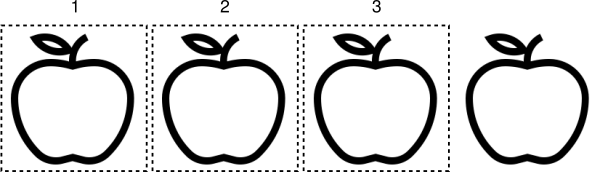
\includegraphics[scale=0.5]{figures/apples_counting.png}
\captionof{figure}{Counting}\label{fig:counting}
\end{figure}

According to the general counting principles, counting is devised to be what we see in \figref{fig:counting}. However, one could easily imagine an operation where, e.g., assigning a number to less than a whole entity or summing up complementary parts of corresponding entities to make up what counts as one is not prohibited. For instance, consider a quantificational operation that satisfies the general counting principle of non-overlap, but violates the principle of integrity. To illustrate this, let us assume illegal counting as depicted in \figref{fig:illegal-counting}.

\begin{figure}[h!]
\centering
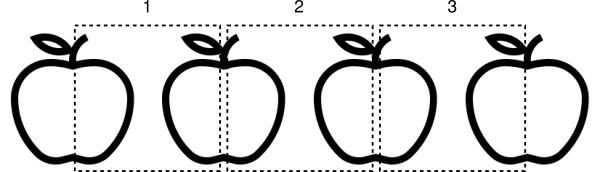
\includegraphics[scale=0.5]{figures/apples_not-counting.png}
\captionof{figure}{Illegal counting}\label{fig:illegal-counting}
\end{figure}

In contrast to \figref{fig:counting}, in this case numbers are associated with arbitrary sums of parts of distinct entities. Notice that those sums can be guaranteed to cover the total volume of all the relevant apples. If this were somehow ensured, in the discussed scenario we could obtain the same number as in \figref{fig:counting}. However, intuitively this operation is very different from counting. It is simply not what we do when we count.

Though the procedure illustrated in \figref{fig:illegal-counting} is not counting, it does not mean that it does not represent another quantificational operation human beings utilize for different purposes. In the next paragraphs, I will discuss what I believe to be the crucial difference between counting and measuring.

\subsection{Counting vs. measuring}\label{sec:counting-vs-measuring}

Intuitively, the difference between counting and measuring relies essentially on the fact that the former is about specifying how many objects of a certain kind there are in a particular context, whereas the latter concerns determining the quantity of a particular substance in relevant measure units. In principle, there are three possible views on the relationship between the two operations in question. The first one reduces measuring to a particular type of counting \citep[e.g.,][]{gil2013numeral}. The intuition behind such an approach is that measure words individuate in terms of quantity \citep{lyons1977semantics}. Consequently, instead of quantification over objects measuring is about counting units determined by measure words. An opposing approach is to view counting as a form of measuring. In particular, counting can be understood as measuring a quantity of an object in terms of natural units \citep{krifka1989nominal,krifka1995common}. Finally, the third option is to postulate that counting and measuring are two independent operations \citep{rothstein2017semantics}. In this study, I adopt the third perspective and present novel evidence in its favor. In particular, I propose that the distinction between counting and measuring can be reformulated in terms of quantificational principles introduced in the previous section. Though both counting and measuring obey the principle of non-overlap and maximality, only the former satisfies the principle of integrity. Measured quantities of a substance cannot overlap in order to ensure that things are not measured twice. Furthermore, a unit of measurement needs to correspond to the maximal quantity of matter to guarantee that measuring is exhaustive. However, only counting is sensitive to the topological make-up of entities it applies to.

To better understand the essence of the distinction, let us consider the following two scenarios. In the first scenario, illustrated in  \figref{fig:measuring-and-integrity}, someone has spilled some liquid on the table in such a way that there are two separate blobs $a$ and $b$ whose volume is one and a half milliliters each. In the second scenario, see \figref{fig:counting-and-integrity}, someone has simply put two cubes $c$ and $d$ on the table. Let us also assume that apart from the liquid and the cubes there is nothing else on the table in each of the cases, respectively.

\begin{figure}[h!]
	\centering
	\begin{tikzpicture}
	\coordinate (a) at (1.0,0.0);
	\coordinate (b) at (5.0,0.0);
	\draw[rounded corners=1mm] (a) \irregularcircle{1cm}{1mm};
	\draw[rounded corners=1mm] (b) \irregularcircle{1cm}{1mm};
	\node at (1.0,0.0) {$a$};
	\node at (5.0,0.0) {$b$};
	\end{tikzpicture}
	\caption{Measuring and integrity}
	\label{fig:measuring-and-integrity}
\end{figure}

\begin{figure}[h!]
	\centering
	\begin{tikzpicture}
	\draw (2.0,0.0) -- (4.0,0.0) -- (4.0,2.0) -- (2.0,2.0) -- (2.0,0.0);
	\draw (6.0,0.0) -- (8.0,0.0) -- (8.0,2.0) -- (6.0,2.0) -- (6.0,0.0);
	\node at (3.0,1.0) {$c$};
	\node at (7.0,1.0) {$d$};
	\end{tikzpicture}
	\caption{Counting and integrity}
	\label{fig:counting-and-integrity}
\end{figure}

Now, let us examine the sentences in \ref{ex:measuring-integrity} and \ref{ex:counting-integrity} describing the situations depicted in Figures \ref{fig:measuring-and-integrity} and \ref{fig:counting-and-integrity}, respectively. The statement in \ref{ex:measuring-integrity} is true despite the fact that one of the three milliliters must be split between a portion of $a$ and a portion of $b$ since each of the blobs consists of one and a half milliliters of liquid. On the other hand, \ref{ex:counting-integrity} is simply false. This contrast shows that units of measurement such as milliliters are not objects. In other words, unlike counting measuring does not care about individuation in terms of integrity and it indeed appears to be a distinct operation.

\ex. English (Guy Tabachnick, p.c.)\label{ex:measuring-counting-integrity}
\a. There are three milliliters of liquid on the table.\label{ex:measuring-integrity}
\b. \#There are three objects on the table.\label{ex:counting-integrity}

I argue that this is because counting is topology-sensitive whereas measuring is not. In other words, in measuring, units of measurement are not required to be assigned only to contiguous entities. There are multiple ways in which one could assign particular milliliters $u_1$, $u_2$, and $u_3$ to particular portions of $a$ and $b$, and \figref{fig:measuring-in-units} illustrates one possible distribution, with $u_2$ corresponding to the volume of liquid of a sum of one-third of $a$ and one-third of $b$. As long as the total volume of $a$ and $b$ equals three milliliters, \ref{ex:measuring-integrity} is true with respect to \figref{fig:measuring-and-integrity}.

\vfill
\begin{figure}[H]
	\centering
	\begin{tikzpicture}
	\coordinate (a) at (1.0,0.0);
	\coordinate (b) at (5.0,0.0);
	\draw[rounded corners=1mm] (a) \irregularcircle{1cm}{1mm};
	\draw[rounded corners=1mm] (b) \irregularcircle{1cm}{1mm};
	\draw[dashed] (1.29,-0.9) -- (1.29,0.9);
	\draw[dashed] (4.7,-0.9) -- (4.7,0.9);
	\node at (0.66,0.0) {$u_1$};
	\node at (3.0,0.0) {$u_2$};
	\node at (5.33,0.0) {$u_3$};
	\end{tikzpicture}
	\caption{Measuring in units}
	\label{fig:measuring-in-units}
\end{figure}
\vfill\pagebreak

Unlike measuring, counting is sensitive to what kind of topological structure entities in its domain have. In parallel to \figref{fig:measuring-in-units}, one could imagine that two-thirds of $c$ correspond to an object $o_1$, one-third of $c$ plus one-third of $d$ make up $o_2$, and the remaining two-thirds of $d$ correspond to $o_3$, as depicted in \figref{fig:counting-objects}. However, this is not how counting typically works. The statement in \ref{ex:counting-integrity} is false with respect to \figref{fig:counting-and-integrity} because counting assigns numbers to integrated individuated entities rather than arbitrary portions thereof.

\begin{figure}[h!]
	\centering
	\begin{tikzpicture}
	\draw (2.0,0.0) -- (4.0,0.0) -- (4.0,2.0) -- (2.0,2.0) -- (2.0,0.0);
	\draw (6.0,0.0) -- (8.0,0.0) -- (8.0,2.0) -- (6.0,2.0) -- (6.0,0.0);
	\draw[dashed] (3.33,0.0) -- (3.33,2.0);
	\draw[dashed] (6.66,0.0) -- (6.66,2.0);
	\node at (2.66,1.0) {$o_1$};
	\node at (5.0,1.0) {$o_2$};
	\node at (7.32,1.0) {$o_3$};
	\end{tikzpicture}
	\caption{Counting objects}
	\label{fig:counting-objects}
\end{figure}

I argue that what the contrast between truth-conditions of \ref{ex:measuring-integrity} and \ref{ex:counting-integrity} discussed above shows is that counting and measuring are in fact two distinct semantic operations, as proposed by \citet{rothstein2017semantics}. The core difference between the two boils down to the fact that counting is topology-sensitive, whereas measuring is not. In other words, it is misleading to think of measuring in terms of counting measure units \citep[pace][]{gil2013numeral}. If it were, similarly to \figref{fig:counting-and-integrity}, we would expect \ref{ex:measuring-integrity} to be false with respect to \figref{fig:measuring-and-integrity}, contrary to fact. 

The distinction gets even more salient if we realize that many numeral phrases can get a measure interpretation.\footnote{See \citet[p. 3]{rothstein2017semantics} for extensive discussion of ambiguities of another sort, namely the alternation between individuating and content readings of container words such as \textit{glass of water}.} For instance, consider the contrast between the scenarios described in \ref{ex:cooking-counting} and \ref{ex:cooking-measuring}. In \ref{ex:cooking-counting-setup}, the numeral phrase \textit{three apples} denotes a plurality of integrated wholes, i.e., distinct individuated objects, and thus it can be felicitously continued by \ref{ex:cooking-counting-continuation}. In other words, since the referents of the phrase satisfy conditions specified by the general counting principles, they can be put in a one-to-one correspondence with numbers.  

\ex. English (Guy Tabachnick, p.c.)\\
	extit{Scenario}: John is cooking with his child. They put three whole apples on a table. John says:\label{ex:cooking-counting}
\a. There are three apples on the table\dots\label{ex:cooking-counting-setup}
\b. Let's count them together: one, two, three.\label{ex:cooking-counting-continuation}

On the other hand, the same phrase in the context of \ref{ex:cooking-measuring} gets a measure reading. Given that the slices in the bowl are placed in such a way that it is impossible to retrieve the original part-whole structures of individual apples, \textit{three apples} does not refer to distinct objects but rather to the volume corresponding to three apples. Consequently, it is distinctively odd to continue the sentence in \ref{ex:cooking-measuring-setup} with \ref{ex:cooking-measuring-continuation}. All things considered, \ref{ex:cooking-counting-setup} presumes an operation depicted in \figref{fig:counting}, whereas \ref{ex:cooking-measuring-setup} does not.

\ex. English (Guy Tabachnick, p.c.)\\
	extit{Scenario}: John is cooking with his child. They sliced three apples and put the slices into a bowl. John says:\label{ex:cooking-measuring}
\a. There are three apples in the bowl\dots\label{ex:cooking-measuring-setup}
\b. \# Let's count them together: one, two, three.\label{ex:cooking-measuring-continuation}

The contrasts discussed above prove that counting indicates integrity or at least easily retrievable traces of integrity of entities it applies to, whereas measuring ignores this factor. Though monotonic systems of measurement track part-whole relations \citep{schwarzschild2002grammar}, they do not seem to be sensitive to topological notions. On the other hand, counting does care about the spatial arrangement of parts making up wholes. This strongly suggests that the two operations in question are distinct from each other. Perhaps, one could argue that despite syntactic as well as semantic differences between numeral phrases and measure phrases \citep[see][]{rothstein2017semantics} counting is a very special case of measuring \citep[see][]{krifka1989nominal,krifka1995common}. In particular, measuring could be thought of as a more general quantificational procedure.  However, for the sake of what this study is about I will assume that measuring and counting are two distinct semantic operations. In the next section, I will propose how general counting principles extend to subatomic quantification.

\subsection{Subatomic quantification}\label{sec:subatomic-quantification}

In Chapters \ref{ch:partitives-and-part-whole-structures}, \ref{ch:exploring-topological-sensitivity}, and \ref{ch:multipliers}, we saw that there is substantial evidence showing that natural language semantics is sensitive to the fact that entities we refer to by means of nominal constructions consist of parts and that there are linguistic means to quantify over such parts. On the other hand, in the previous section I postulated the general counting principles of non-overlap, maximality, and integrity. So far, we have seen that there are good reasons to believe that these quantificational constraints capture what humans do when they count objects. In this section, I argue that the proposed set of rules constitutes a universal mechanism that can be applied not only to whole individuals but also when counting parts of objects. In other words, I posit that subatomic quantification is subject to the very same constraints as quantification over wholes.

Analogously to what we saw in \figref{fig:counting}, counting at the subatomic level presumes mereological maximality and topological integrity of entities subject to quantification. Typically, counting is sensitive to the fact that some parts are cognitively more salient within the part-whole structure of an object than others. This seems to correspond to what \citet{champollion_krifka2016mereology} call structured parthood as well as to the distinction between specific and arbitrary subdivisions of a whole into parts introduced in philosophical considerations, as already mentioned in Chapter \ref{ch:introduction} \citep[e.g.,][]{krecz1986parts,markosian1998brutal,jennings2010against}. Notice that what counts as a cognitively salient part can vary with respect to the context. For instance, consider the two sentences in \ref{ex:cognitively-salient-parts}. 

\ex. English (Guy Tabachnick, p.c.)\label{ex:cognitively-salient-parts}
\a. Both parts of the teddy bear are painted.\label{ex:cognitively-salient-parts-both}
\b. Two parts of the teddy bear are painted.\label{ex:cognitively-salient-parts-two}

Assume John's daughter has a teddy bear called Fuzzy Wuzzy. In a situation where she has covered Fuzzy Wuzzy's entire left half with red paint and its entire right half with black paint, John might want to say \ref{ex:cognitively-salient-parts-both}. In such a case, the total volume of matter making up the teddy bear is partitioned in such a way that the cognitively salient parts are its left half and its right half.\footnote{The sentence in \ref{ex:cognitively-salient-parts-both} appears to be slightly degraded due to the fact that instead of \textit{part} a more accurate partitive word, i.e., \textit{half}, could have been used. Many thanks to Guy Tabachnick for discussing the English examples with me.} On the other hand, in a scenario where John's daughter painted Fuzzy Wuzzy's left paw red and its right paw black, the count explicit partitive in \ref{ex:cognitively-salient-parts-two} refers to the teddy bear's body parts. Nevertheless, what cognitively salient parts have in common is that given a particular context they are disjoint. This brings us to the relevance of the principle of non-overlap in subatomic quantification.\largerpage

Since there are numerous ways in which one could divide an object into parts, there are multiple portions of matter of which the property of being part of that object holds. For instance, \figref{fig:overlapping-parts} illustrates a number of entities the phrase \textit{part of the apple} could refer to. Notice that none of them is disjoint from the others, i.e., all of them share a part with at least one other part. However, the principle of non-overlap states that such entities cannot be counted. Similarly to arbitrary portions of mass, e.g., juice, arbitrary parts of an apple avert individuation since they are not well-defined bounded integrated objects and it is virtually impossible to distinguish them from other parts. This means that not all parts are equal with respect to countability. Some of them are countable, whereas others are not. Crucially, only those divisions of a whole into parts can be enumerated that are perceived as involving only non-overlapping parts.

\begin{figure}[h!]
\centering
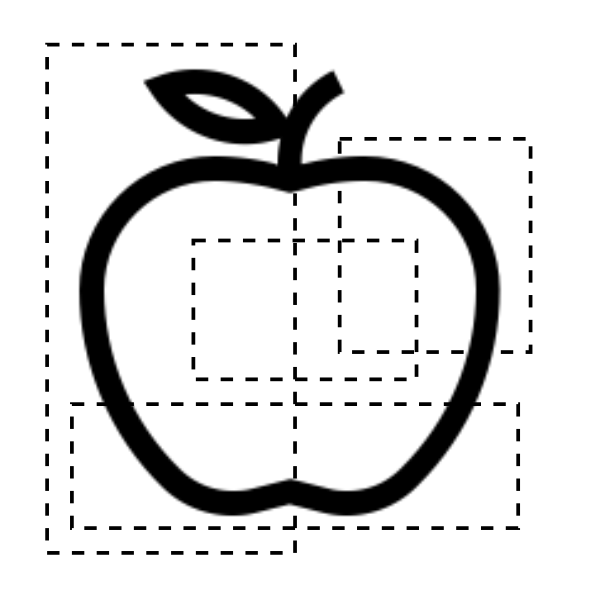
\includegraphics[scale=0.5]{figures/apple_overlap.png}
\captionof{figure}{Overlapping parts}\label{fig:overlapping-parts}
\end{figure}

Another issue concerns the principle of maximality. What counts as part of an object can also consist of smaller parts. Notice that such parts of parts also satisfy the property of being part of that object. However, the general counting principles require that only entities in their mereological entirety can be associated with a number. This means that once a particular division of an individual into parts has been executed in a given counting context, those parts are immutable and are treated as objects in their own right. Consequently, the principle of maximality applies as it would in a situation when one counts whole individuals. In other words, given a partition, non-overlapping parts are assumed to be maximal with respect to how the whole has been divided.

Finally, as we saw in the previous section, countability is also governed by the principle of integrity. However, as we saw in Chapter \ref{ch:exploring-topological-sensitivity}, extensions of expressions referring to parts of objects do not necessarily involve topological commitments, i.e., parts need not be continuous. For instance, let us consider explicit entity partitives. There is definitely a sense in which two or more separated portions of matter within an object are part of that object, and thus a topology-neutral explicit entity partitive construction would be true of such a configuration. Nevertheless, as any arbitrary sum such entity is not countable since associating it with a number would clearly violate the principle of integrity. Therefore, only sets including parts that are mereologically maximal integrated entities that do not overlap can be enumerated. In other words, only a subset of possible divisions of an object is fit for counting.

Having this in mind, let us see how the general counting principles apply in the context of subatomic quantification. For this purpose, let us assume John's daughter wants to count parts of her teddy bear Fuzzy Wuzzy. \figref{fig:counting-of-parts} represents an exemplary situation that intuitively fits what we expect from counting. 

\begin{figure}[h!]
\centering

\includegraphics[scale=0.5]{figures/toy_counting-parts.png}
\captionof{figure}{Counting of parts}\label{fig:counting-of-parts}
\end{figure}

The operation illustrated above assigns numbers to cognitively salient non-overlapping parts of Fuzzy Wuzzy, namely its ear, leg, and paw. Those parts constitute mereologically maximal and integrated entities, i.e., though they are elements of a larger whole, when counted they are treated as objects in their own right. This means that, e.g., number 1 is associated with Fuzzy Wuzzy's whole ear and there is no part of that ear that is left out. Also, an ear is a continuous part that comes in one piece. To sum up, since the depicted division of the teddy bear consists of elements that are disjoint, maximal, and integrated, all the counting principles are satisfied and the set of parts can be enumerated.

On the other hand, one could imagine another operation, e.g., one such as that illustrated in \figref{fig:illegal-counting-of-parts}. Though it is definitely logically possible, it seems weird and would intuitively be rejected as counting. There are two reasons why this is so. The first reason is that the indicated ear and leg do not constitute a continuous integrated part that would be cognitively salient. Therefore, assigning them the number 1 violates the principle of integrity. In other words, there is a sense in which an ear and a leg are part of the teddy bear, but they are not \textit{a part} of it and only entities that can be considered as such can satisfy the countability condition. The second reason is that the marked paw is not disjoint with the right half of the teddy bear which of course violates the principle of non-overlap. Given the division in \figref{fig:illegal-counting-of-parts}, the paw in question would be counted twice and since counting requires that an entity can be associated with a number once and once only, the depicted operation fails to satisfy the general counting principles and represents what I call illegal counting at the subatomic level, recall \figref{fig:illegal-counting}.

\begin{figure}[h!]
\centering

\includegraphics[scale=0.5]{figures/toy_not-counting-parts.png}
\captionof{figure}{Illegal counting of parts}\label{fig:illegal-counting-of-parts}
\end{figure}

All things considered, counting at the subatomic level presumes assigning numbers to salient parts of a whole constituting disjoint integrated entities that are maximal with respect to a given partition. In other words, once it is decided what counts as a part, it is treated as an individuated object in its own right and all discussed constraints concerning counting apply. The key conclusion is that there is one universal mechanism governing quantification over wholes as well as subatomic quantification, and exploring the latter can reveal some fundamental properties of countability in general that otherwise might be difficult to recognize.

\section{Summary}\label{sec:summary-ch5}

In this chapter, I provided a general conceptual framework that will serve as a basis for developing a formal account for subatomic quantification in natural language. I suggested how the linguistic evidence presented in Chapters \ref{ch:partitives-and-part-whole-structures}, \ref{ch:exploring-topological-sensitivity}, and \ref{ch:multipliers} correlates with findings in cognitive psychology. In particular, in the first part of the chapter I reviewed several representative studies in the research indicating the following. First, there is compelling evidence that humans possess an innate ability to perceptually distinguish between objects, i.e., bounded integrated entities, and substances, i.e., shapeless scattered portions of matter, and that this contrast correlates with the mass/count distinction in grammar, though the correspondence is imperfect. Specifically, integrated solid things are predictably referred to by count nouns, but there is a class of mass terms that also refer to objects. Importantly, the object/mass distinction is not based on ontological properties of entities in some objective sense but rather it is construed by human cognition. Second, the ability to simultaneously perceive parts as elements of a whole and a whole as a collection of parts manifests itself in early childhood. The capacity to intuitively distinguish between parts and wholes guides vocabulary acquisition. Finally, human number sense appears to be sensitive to whether counted items are conceptualized as integrated objects. Experimental evidence shows that young children always count each separate physical entity as one. Even if they are instructed to do otherwise or given clues that two elements might be considered one broken thing, they ignore them and simply cannot avoid counting contiguous entities. This suggests that further development of quantification in older humans rests on a mechanism  individuating singular objects in terms of spatial integrity.

In the second part of this chapter, I presented the three claims that constitute the conceptual core of this study. I postulated that natural language is sensitive to how the spatial relationship holding between parts of a particular entity is conceptualized. The relevance of the topological notion of integrity manifests itself primarily in how the nominal lexicon is classified into different grammatical categories. In particular, count singular nouns prototypically designate integrated wholes, i.e., encode information concerning a particular spatial configuration of parts their referents consist of, whereas plurals denote arbitrary sums thereof, i.e., presuppose integrated wholes as parts but impose no topological constraints on them.

The second claim regards what I call the general counting principles. I posit that counting is a special kind of quantificational operation that presumes certain properties of entities that are put in a one-to-one correspondence with numbers. Specifically, the principle of non-overlap guarantees that enumerated entities are disjoint, and thus no thing is counted twice. On the other hand, the principle of maximality requires that numbers are associated with entities in their mereological entirety, i.e., no part is left out. Finally, the principle of integrity ensures that what can be counted needs to be conceptualized as something that comes in one piece. This constraint excludes arbitrary sums of individuals as well as scattered entities such as substances. Altogether, the general counting principles guarantee that sets that can be enumerated consist only of elements that are discrete object.

The final claim extends the general counting principles to subatomic quantification. In other words, I postulate the quantificational mechanism described above is a universal mechanism that can apply both at the level of wholes and at the level of parts. In the next chapter, I will introduce a theory of wholes called mereotopology in which the formal account for subatomic quantification will be grounded. In particular, it will enable us to capture various subtle topological distinctions including the intuitive notion of an integrated whole as opposed to an arbitrary sum of parts. This will provide means to model not only the fact that some entity is part of something else but also how individual parts are spatially arranged within a whole configuration.

\chapter{Theory of parts and wholes}\label{ch:theory-of-parts-and-wholes}

Given the conceptual background described in the previous chapter, an account for subatomic quantification is supposed to capture the intuitive notions of parthood and integrity. In this chapter, I will introduce a theory of parts and wholes that provides the formal apparatus devised to model both concepts. This theory is usually referred to as mereotopology and as suggested by the name it involves two interrelated components. In the following sections, I will first introduce standard mereology, its axioms, and advantages. Next, I will turn to its limitations and discuss how it can be extended with topological notions such as connectedness. As a result, the sophisticated mereotopological framework to be presented will allow us to model integrated wholes as opposed to other types of entities. The mereotopological distinctions to be developed will play a crucial role in the formal account for subatomic quantification in natural language that I will propose in the next chapter.

\section{Mereology}\label{sec:mereology}

\textsc{mereology} (from the Greek $\mu\epsilon\rho o\zeta$ `part') is the study of parthood, i.e., relations between part and whole as well as between parts within a whole. It was proposed by \citet{lesniewski1916podstawy} and further developed by \citet{leonard_goodman1940calculus} and \citet{goodman1951structure} as an alternative to set theory. In particular, since set theory is founded on the notion of set membership $\in$, i.e., the relation between an element and a set, it distinguishes between a singleton set and its member, i.e. $\{a\} \neq a$. For this reason, the nominalist tradition from which mereology stems has considered set theory as ontologically suspect. In order to avoid potentially problematic ontological assumptions, mereology does not postulate abstract entities such as sets. Instead, the meronomic relation of parthood is postulated as the primitive notion of the theory. Therefore, in mereology there is no need to draw the distinction between a singleton set and its member. Though historically mereology was viewed as equivalent to a rejection of set theory, since at least \citet{eberle2012nominalistic} it has been gradually recognized that employing mereological concepts is possible irrespective of one's ontological position concerning sets.

The part-whole relation can hold between portions of masses, parts of individuals, members of groups, locations, events, times, and even abstract entities, as depicted in \tabref{tab:examples-wholes-part}  \citep[see][]{simons1987parts,winston_chaffin_herrmann1987taxonomy}. It is a prominent notion in how the world appears to be structured, how human beings perceive things and talk about things. Therefore, mereology plays an important role in ontology, cognitive psychology, and natural-language semantics. Since \citeposst{quine1960word} discussion of mass nouns as scattered objects (a clearly mereological concept), considering countability in mereological terms became standard in philosophy (see especially \citealt{sharvy1980more} for a treatment of mass definite descriptions in this spirit). However, it was \citet{link1983logical} who introduced formal mereology to linguistics in his lattice-theoretic approach to pluralities.\largerpage

\begin{table}[h!]
\centering
\begin{tabular}{ll}
\lsptoprule
\textsc{whole}   & \textsc{part}     \\ \midrule
some horses  & a subset of them          \\
a quantity of water & a portion of it         \\
John, Mary, and Bill         & John          \\
some jumping events       & a subset of them        \\
a running event from A to B         & its part from A halfway towards B  \\
a temporal interval & its initial half  \\
a spatial interval          & its northern half \\ \lspbottomrule
\end{tabular}
\caption{Examples of wholes and parts \citep[p. 12]{champollion2017parts}}
\label{tab:examples-wholes-part}
\end{table}

There are different ways in which one could spell out mereological intuitions and axiomatize the parthood relation (see, e.g., \citealt{simons1987parts,casati_varzi1999parts,varzi2016mereology} for thorough surveys of the field). However, in this chapter I will discuss only a system that gives rise to algebraic structures, i.e., sets with binary operations defined on them, which is often referred to as classical extensional mereology. For brevity, however, I will simply call it standard mereology since it is considered to be a standard in mereology (though see, e.g., \citealt{rescher1955axioms} for an alternative proposal) and is most commonly used in formal semantics for natural language (e.g., \citealt{link1983logical,krifka1989nominal,landman2000events,champollion2017parts}, to name just a few prominent approaches). The axiomatization of standard mereology presented here largely  follows the extensive discussions provided by \citet{simons1987parts} and \citet{casati_varzi1999parts} as well as the encyclopedic entry on linguistic applications of mereology by \citet{champollion_krifka2016mereology}. To avoid terminological confusion I will follow \citet{grimm2012number} in distinguishing between \textsc{individuals}, i.e., a pre-theoretic notion regarding well-defined physical entities, and \textsc{m-individuals}, i.e., objects in the mereological sense.

The most common view on the axiomatization of mereology takes the concept of \textsc{part} ($\sqsubseteq$) to be the basic notion. The part-of relationship $\sqsubseteq$ is the primitive relation which is reflexive, transitive, and antisymmetric.\footnote{I use the symbol $\sqsubseteq$ following \citet{landman1989groupsi,landman1989groupsii,landman2000events}. Other authors use $\leq$ instead. The main motivation behind this notational decision is to avoid potential confusion with the `less than or equal to' relation between numbers.} The axioms given in \ref{ex:reflexivity}--\ref{ex:antisymmetry} constrain $\sqsubseteq$ to be a partial order.

\ex. Reflexivity \citep[p. 515; adapted]{champollion_krifka2016mereology}\label{ex:reflexivity}\\
{$\forall x[x\sqsubseteq x]$}\\
(Every thing is part of itself.)

\ex. Transitivity \citep[p. 516; adapted]{champollion_krifka2016mereology}\label{ex:transitivity}\\
{$\forall x\forall y\forall z[(x\sqsubseteq y \wedge y\sqsubseteq z) \rightarrow x\sqsubseteq z]$}\\
(Any part of any part of a thing is itself part of that thing.)

\ex. Antisymmetry \citep[p. 516; adapted]{champollion_krifka2016mereology}\label{ex:antisymmetry}\\
$\forall x\forall y[(x\sqsubseteq y\wedge y\sqsubseteq x)\rightarrow x=y]$\\
(Two distinct things cannot both be part of each other.)

Given that the primitive $\sqsubseteq$ relation is defined in such a way that an m-individual is part of itself, it might be useful to introduce an auxiliary notion of parthood which is not reflexive. The formula in \ref{ex:proper-part} provides the definition of \textsc{proper part} ($\sqsubset$).

\ex. Proper part \citep[p. 36]{casati_varzi1999parts}\label{ex:proper-part}\\
$x \sqsubset y \eqdef x \sqsubseteq y \wedge \neg(y \sqsubseteq x)$\\
(A proper part of a thing is a part of a thing that is distinct from it.)

Furthermore, one might also want to account for the fact that entities can share parts. For this reason, an ancillary relation \textsc{overlap} (\cnst{o}) can be defined, as in \ref{ex:overlap}.\footnote{I use the $\cnst{o}(x,y)$ notation following \citet{casati_varzi1999parts}, \citet{varzi2007spatial}, and \citet{grimm2012number}. Other authors use $x \circ y$ instead.} From a mereological point of view, identity can be understood as a special case of overlap.

\ex. Overlap \citep[p. 516; adapted]{champollion_krifka2016mereology}\label{ex:overlap}\\ 
$\cnst{o}(x,y) \eqdef \exists z[z \sqsubseteq x \wedge z \sqsubseteq y]$\\
(Two things overlap if and only if they share a part.)

The parthood relation together with the derived notions of proper part and overlap constitute the core of standard mereology. However, without any further constraints the system developed so far gives rise to structures which have been traditionally dismissed as objects that a theory of part-whole relations should represent. For instance, \figref{fig:object-solitary-proper-part} illustrates a mereological relation between the m-individuals $a$ and $b$ such that $b$ is a proper part of $a$ and there is no other proper part of $a$.\footnote{The line represents $\sqsubseteq$ with the m-individual corresponding to the lower node being part of the m-individual corresponding to the higher node.} 

\begin{figure}[h!]
\centering
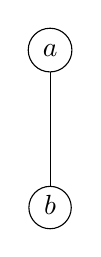
\begin{tikzpicture}[every node/.style={draw=black,thin,circle,inner sep=1pt,font=\strut}, node distance=2cm]
  \node (a) {$a$};
  \node (b) [below of=a] {$b$};
  \draw (a) -- (b);
\end{tikzpicture}
\caption{Object with a solitary proper part}
\label{fig:object-solitary-proper-part}
\end{figure}

Similarly, \figref{fig:objects-share-all-parts} depicts a model in which two distinct m-individuals $a$ and $c$ both share all parts. Though such models are allowed within the system, intuitively they are not what a theory of parts and wholes should account for. To remedy this, further constraints have to be introduced. 

\begin{figure}[h!]
\centering
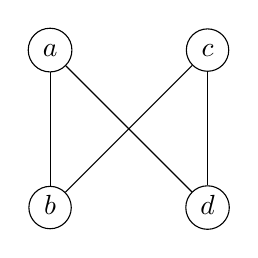
\begin{tikzpicture}[every node/.style={draw=black,thin,circle,inner sep=1pt,font=\strut}, node distance=2cm]
  \node (a) {$a$};
  \node (b) [below of=a] {$b$};
  \node (c) [right of=a] {$c$};
  \node (d) [right of=b] {$d$};
  \draw (a) -- (b);
  \draw (a) -- (d);
  \draw (b) -- (c);
  \draw (c) -- (d);
\end{tikzpicture}
\caption{Objects sharing all parts}
\label{fig:objects-share-all-parts}
\end{figure}

Standard mereology can be devised in order to restrict how an m-individual can be decomposed into parts. In particular, an additional axiom can be added that constrains mereological objects in such a way that every proper part must be supplemented by another disjoint part. In other words, there is always a mereological difference between a whole and its proper parts. An extension known as \textsc{remainder principle} or \textsc{supplementation}, see \ref{ex:supplementation}, guarantees that m-individ\-uals cannot consist of a single proper part, and thus models such as that in  \figref{fig:object-solitary-proper-part} are ruled out.\largerpage[2]

\ex. Supplementation \citep[p. 36]{casati_varzi1999parts}\label{ex:supplementation}\\
$x \sqsubset y \rightarrow \exists z[z \sqsubseteq y \wedge \neg\cnst{o}(z,x)]$\\
(Whenever a thing has a proper part, it has more than one.)

However, supplementation is insufficient to exclude structures like the one in \figref{fig:objects-share-all-parts}, and thus another extension needs to be implemented in order to ban them. Given $\sqsubseteq$, the notion of \cnst{sum} can be defined. Sums are devised to capture a pretheoretical concept of collections, i.e., the result of grouping several entities together. In natural language, conjoined terms and definite descriptions like \textit{the water} have been analyzed in terms of sums. In particular, in his influential paper \citet{link1983logical} treats expressions such as \textit{John and Mary} as referring to the sum of two individuals, namely John and Mary. In a similar vein, \citet{sharvy1980more} proposes that a definite expression such as \textit{the water} denotes the sum of all water. Here I will follow the classical definition of sum due to \citet{tarski1929fondements}, as presented in \ref{ex:sum} (for alternative definitions, see \citealt{simons1987parts,casati_varzi1999parts}).

\ex. Sum\label{ex:sum} \citep[p. 517; adapted]{champollion_krifka2016mereology}\\
$\cnst{sum}(x,P) \eqdef \forall y[P(y) \rightarrow y \sqsubseteq x] \wedge  \forall z[z \sqsubseteq x \rightarrow \exists z'[P(z') \wedge \cnst{o}(z,z')]]$

In prose, a sum of (the things in) a set $P$ is a thing that consists of everything in $P$ and whose parts each overlap with something in $P$. Since the part structures in standard mereology are closed under sum formation, for any two individuals there is also a sum of those two individuals. This is ensured by \textsc{uniqueness of sums}, which requires two things composed of the same parts to be identical, see \ref{ex:uniqueness-sums}. This principle excludes structures such as the one in \figref{fig:objects-share-all-parts}. Since $b$ and $d$ form two different sums, namely $a$ and $c$, uniqueness of sums is violated and the model is ruled out, as desired. Notice also that introducing uniqueness of sums makes the axioms of reflexivity and antisymmetry redundant since any transitive relation that satisfies uniqueness of sums is provably reflexive and antisymmetric \citep[see][]{hovda2009classical,champollion2017parts}. The axioms have been discussed for completeness though.

\ex. Uniqueness of sums \citep[p. 517; adapted]{champollion_krifka2016mereology}\label{ex:uniqueness-sums}\\
$\forall P[P \neq \varnothing \rightarrow \exists !z\ \cnst{sum}(z,P)]$\\
(Every non-empty set has a unique sum.)

Finally, the additional notions \textsc{binary sum} and \textsc{generalized sum} can be derived, as given in \ref{ex:binary-sum} and \ref{ex:generalized-sum}, respectively.\footnote{Again, I follow \citet{landman1989groupsi,landman1989groupsii,landman2000events} in the use of the symbols $\sqcup$ and $\bigsqcup$, respectively, which correspond to the symbols $\oplus$ and $\bigoplus$ one can often find in the literature.} The former operation allows us to refer explicitly to the sum of two m-individuals, whereas the latter to the sum of an arbitrary set.

\ex. Binary sum \citep[p. 518; adapted]{champollion_krifka2016mereology}\label{ex:binary-sum}\\
$x \sqcup y \eqdef \iota z\ \cnst{sum}(z,\{x,y\})$

\ex. Generalized sum \citep[p. 518; adapted]{champollion_krifka2016mereology}\label{ex:generalized-sum}\\
$\bigsqcup X \eqdef \iota z\ \cnst{sum}(z,X)$, where $X$ is any non-empty set

Consequently, the meaning of the coordinate phrase \textit{John and Mary} can be represented as $j \sqcup m$, whereas the semantics of the definite description \textit{the water} is represented as $\bigsqcup\textsc{water}$.

Alongside philosophical arguments for standard mereology, a significant advantage of this framework is that it involves a well-understood algebraic structure. In particular, as demonstrated by \citet{tarski1935grundlegung} models delivered by mereology are essentially isomorphic to Boolean algebras with their bottom element removed, or equivalently complete semi-lattices without the null element \citep[see also][]{pontow_schubert2006mathematical}.\footnote{The reason is that standard mereology does not allow for an object that is part of everything and since the empty set is a subset of every other set, it must be eliminated.} \figref{fig:semi-lattice} gives an example of a mereological structure licensed by standard mereology. Note that it is isomorphic to the powerset of the set $\{a,b,c\}$ with the bottom element removed. 

\begin{figure}[h!]
\centering
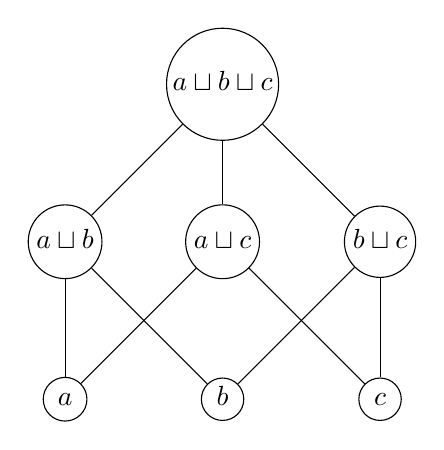
\begin{tikzpicture}[every node/.style={draw=black,thin,circle,inner sep=1pt,font=\strut}, node distance=2cm]
  \node (abc) {$a \sqcup b \sqcup c$};
  \node (ac) [below of=abc] {$a \sqcup c$};
  \node (ab) [left of=ac] {$a \sqcup b$};
  \node (bc) [right of=ac] {$b \sqcup c$};
  \node (a) [below of=ab] {$a$};
  \node (b) [right of=a] {$b$};
  \node (c) [right of=b] {$c$};
  \draw (a) -- (ab);
  \draw (a) -- (ac);
  \draw (b) -- (ab);
  \draw (b) -- (bc);
  \draw (c) -- (ac);
  \draw (c) -- (bc);
  \draw (ab) -- (abc);
  \draw (ac) -- (abc);
  \draw (bc) -- (abc);
\end{tikzpicture}
\caption{Semi-lattice}
\label{fig:semi-lattice}
\end{figure}

I will follow the well-established tradition in the semantic literature and refer to such models as complete semi-lattices. However, as pointed out by \citet{champollion2017parts} due to the lack of the null element the use of the term \textit{complete} is rather inadequate since it deviates from standard mathematical practice \citep[see also][]{landman1989groupsi}. The definition of such a structure is given in \ref{ex:complete-semi-lattice}.

\ex. Semi-lattice \citep[p. 17; adapted]{champollion2017parts}\\
Let $S$ be a set and $\sqsubseteq$ be a relation from $S$ to $S$. A pair $\langle S,\sqsubseteq \rangle$ is called a complete semi-lattice iff $\sqsubseteq$ satisfies the axioms of transitivity and uniqueness of sums.\label{ex:complete-semi-lattice}

Before we move on to the discussion of the limits of standard mereology that seem to have posed some serious problems in the study of natural language semantics adopting lattice-theoretic approaches, let us briefly contemplate some correspondences between mereology and set theory.

\subsection{Mereology vs. set theory}\label{sec:mereology-set-theory}

It can be easily noted that the notion of parthood in standard mereology has basically the same properties as the subset relation in standard set theory. Therefore, since $\sqsubseteq$ and $\subseteq$ are very much alike, there are a number of deep correspondences between the two axiom systems, some of which are illustrated in \tabref{tab:correspondences-mereology-set-theory}. Consequently, in many contexts it might be convenient to regard sums as sets, and a question arises on why mereology is preferable over set theory in modeling pluralities in natural language semantics.

\begin{table}[h]
\fittable{\begin{tabular}{lll}
\lsptoprule
\textsc{property}          & \textsc{mereology}    & \textsc{set theory}     \\ \midrule
reflexivity       & $x \sqsubseteq x$  & $x \subseteq x$ \\
transitivity      & $x \sqsubseteq y \wedge y \sqsubseteq z \rightarrow x \sqsubseteq z$     & $x \subseteq y \wedge y \subseteq z \rightarrow x \subseteq z$               \\
antisymmetry      & $x \sqsubseteq y \wedge y \sqsubseteq x \rightarrow x = y$                            & $x \subseteq y \wedge y \subseteq x \rightarrow x = y$               \\
interdefinability & $x \sqsubseteq y \Leftrightarrow x \sqcup y = y$                               & $x \subseteq y \Leftrightarrow x \cup y = y$                \\
unique sum/union  & $P \neq \varnothing \rightarrow \exists !z[\cnst{sum}(z,P)]$           & $\exists !z[z = \cup P]$               \\
associativity     & $x \sqcup (y \sqcup z) = (x \sqcup y) \sqcup z$                 & $x\cup (y\cup z)=(x\cup y)\cup z$               \\
commutativity     & $x \sqcup y = y \sqcup x$                                           & $x \cup y = y \cup x$               \\
idempotence       & $x \sqcup x = x$                                                      & $x \cup x = x$               \\
unique separation & $x \sqsubset y \rightarrow \exists !z[x\sqcup z = y \wedge \neg \cnst{o}(x,z)]$ & $x \subset y \rightarrow \exists !z[z = y - x]$ \\ \lspbottomrule
\end{tabular}}
\caption{Correspondences between mereology and set theory \citep[p. 519; adapted]{champollion_krifka2016mereology}}
\label{tab:correspondences-mereology-set-theory}
\end{table}

\begin{sloppypar}
Though early approaches to the semantics of plural expressions were grounded in set theory \citep{bennet1974some,hausser1974quantification}, a substantive body of contemporary research embraces systems based on the notion of parthood. The original motivation behind preferring mereology over set theory in the logic of plurality developed by \citet{link1983logical,link1998algebraic} was formulated on philosophical grounds. In particular, \citeauthor{link1998algebraic} argues that the traditional set-up of semantics taking the domain of individuals to be simply a non-empty set fails to represent various relations between objects. In other words, it is devised to capture only flat domains and cannot account for structured domains, as in modeling natural language. In terms of ontology, \citeauthor{link1998algebraic} describes his position as ``relative nominalism'' and argues that a set-theoretic approach is not desirable because by treating pluralities as sets, it commits us to assuming additional abstract objects. On the other hand, since in a mereological framework pluralities are treated on par with singularities as individuals, such an approach bears no additional ontological commitments, and thus is to be preferred.\footnote{But see \citet{landman1989groupsi} for a discussion challenging such a view.}
\end{sloppypar}

Another arguable advantage of using mereology rather than set theory in plural semantics is that it conveniently allows us to distinguish type-theoretically between the denotations of common nouns, i.e., set-denoting expressions of type $\langle e,t\rangle$, and plural individuals, i.e., individual-denoting expressions of type $e$ \citep[see also][]{vaillette2001flexible,champollion2017parts}. Due to the lack of sums set-theoretic approaches to pluralities conflate the meanings of these two types of expressions which can be considered an undesired result. 

A prominent linguistic application of standard mereology is the theory developed by \citet{champollion2017parts}, who adopts the order-theoretic perspective and treats $\sqsubseteq$ as primitive. On the other hand, \citet{krifka1998origins} derives $\sqsubseteq$ from $\sqcup$. Other influential theories that were intended to characterize standard mereology were developed by \citet{link1983logical,link1998algebraic} and \citet{landman1989groupsi,landman1991structures,landman2000events}.\footnote{But see a scrupulous review by \citet{hovda2009classical} who demonstrates in detail that these systems contain certain flaws, which result in them failing to describe standard mereology, as intended.}

\subsection{Limits of mereology}\label{sec:limits-of-mereology}

As has been pointed out by many authors, there is independent motivation for extending standard mereology with auxiliary notions. One factor concerns the criticism mereology faced with respect to its inadequacy in modeling objects in the real world. In particular, mereology is committed to unrestricted sum formation and as such it is insufficient to capture what it means to be a whole. This results in diametrical discrepancies between intuitions regarding the nature of entities in the world and objects mereology actually delivers. To use \citeposst{casati_varzi1999parts} example, imagine a cup and broken glass. Intuitively, the former constitutes an object, i.e., an individuated whole, something that counts as one, whereas the latter is just a collection of shards. However, this distinction cannot be captured by describing entities purely in terms of parthood. This is because in mereology for every whole there is a set of parts and to every arbitrary collection of parts there is their sum, i.e., a complete whole. As a result, a cup and broken glass have the very same mereological status. In other words, the allowance of scattered entities makes it impossible to differentiate between them and individuals constituting integrated wholes. Consequently, mereology has faced criticism that in principle it fails as a theory of individuals.

As suggested by \citet{grimm2012number}, it is very likely that at least some of the shortcomings of mereological approaches to pluralities and countability in natural language may be due to the general flaws of standard mereology in attempting to capture what it means to be a whole. Arguably, extending standard mereological frameworks with additional notions in order to develop a better theory of objects, as proposed, e.g., by \citet{casati_varzi1999parts}, may provide superior tools for semantic treatments of quantification in natural language. As already signaled, a challenging problem concerns the requirement of unrestricted sum formation which states that for every two elements in the domain, there is a plural individual corresponding to the sum of those two elements. Specifically, the ontological status of such a plural entity has often been disputed. As wittily put by \citet{landman1989groupsi}, if three children messed up the living room, the correct answer to the question ``How many individuals were involved in messing up the living room?'' is ``three'', whereas ``seven'' clearly seems incorrect.\footnote{See also \citet{cresswell1985review}.} However, if pluralities were conceptualized as having the same ontological status as singular individuals, we would expect this answer to be adequate since that number includes all distinct sums of the children in question. In other words, if the children were Anne, Betty, and Carl, i.e., $a$, $b$, and $c$ respectively, then 7 is the number of the elements of the set consisting of all entities that are part of the total sum of the children, i.e., $\{a, b, c, a \sqcup b, a \sqcup c, b \sqcup c, a \sqcup b \sqcup c\}$. The fact that natural language does not allow for quantification over arbitrary sums suggests that the way individual objects are conceptualized differs from how we see pluralities of objects. However, standard mereology lacks notions fine-grained enough to distinguish between objects that come in one piece and entities that do not.

The next section will introduce an extension of standard mereology within which more fine-grained notions can be defined. These notions will enhance mereology in that in addition to parthood they will allow us to capture also the topological configuration of entities making up a particular sum, i.e., their spatial arrangement. In other words, the topological extension will make it possible to discriminate between scattered entities and wholes that come in one piece.

\section{Mereotopology}\label{sec:mereotopology}

\textsc{topology} (from the Greek $\tau o\pi o\zeta$ `place') is the study of those properties of space that are unaffected by continuous deformations of shape or size of figures such as stretching or bending, as opposed to tearing or gluing. Two of the crucial notions studied in the field are connectedness and compactness. Important contributions to the early development of topology were made by \citet{frechet1906quelques}, \citet{hausdorff1914grundzuge}, and \citet{kuratowski1922operation}. 

Theories that extend standard mereology with topological relations are  known as \textsc{mereotopology}. Though early attempts to formalize such a system trace back to \citet{whitehead1920concept,whitehead1929process}, for many decades there was no continuation in the systematic study of mereotopological issues until relatively recent work in artificial intelligence began to investigate the interaction between mereological and topological notions in order to develop formal representations of spatial relations such as \textsc{near} or \textsc{inside}. Consequently, new developments in philosophy and ontological modeling  \citep[e.g.,][]{clarke1981calculus,smith1996mereotopology,roeper1997region} motivated the extension of standard mereology with topological relations in order to advance an improved theory of objects.

Though topological notions have been widely used within the study of locatives \citep[e.g.,][]{clark1973space,herskovits1985semantics,zwarts_winter1997semantic,kracht2002semantics}, it was not until \citet{grimm2012degrees,grimm2012number} that mereotopology was introduced to natural language semantics.\footnote{Mereotopology has been further applied to particular topics concerning countability in \citet{lima2014all} and \citet{grimm_docekal-toappear-counting}. The theory has also inspired approaches that do not develop full-fledged mereotopological accounts but employ some spatial relations in order to capture certain issues relating to individuation such as \citet{scontras2014semantics,scontras2017new}, \citet{sutton_filip2017probabilistic,sutton_filip2017individuation}, \citet{henderson2017swarms}, and \citet{krifka-toappear-individuating}.} In this chapter, I will define basic topological concepts and review how they interact with mereological notions as discussed by \citet{casati_varzi1999parts} and adopted for the semantic treatment of countability by \citet{grimm2012degrees,grimm2012number}.

There are two main approaches with respect to relating mereology and topology: (i)~choosing mereology as a basic level and augmenting it with topological notions, or (ii)~choosing topology as a basic level and adding mereological relations. I will follow \citet{grimm2012number}, who employs a technique of simply extending mereology with topological notions. In particular, he adopts the approach developed in \citet{casati_varzi1999parts}, which I will describe in the following paragraphs.\largerpage

The crucial topological notion for the purpose of this study is \textsc{connectedness} (\cnst{c}). This relation is introduced in such a way that it interacts with other definitions and axioms of standard mereology. Connectedness is reflexive and symmetric, as defined in the axioms in \ref{ex:connectivity-reflexivity} and \ref{ex:connectivity-symmetry}.

\ex. Reflexivity \citep[p. 52; adapted]{casati_varzi1999parts}\label{ex:connectivity-reflexivity}\\
$\forall x[\cnst{c}(x,x)]$\\
(Every thing is connected to itself.)
	
\ex. Symmetry \citep[p. 52; adapted]{casati_varzi1999parts}\label{ex:connectivity-symmetry}\\
$\forall x\forall y[\cnst{c}(x,y) \rightarrow \cnst{c}(y,x)]$\\
(If $x$ is connected to $y$, then $y$ is also connected to $x$.)

Notice, however, that unlike the parthood relation $\sqsubseteq$, as defined in standard mereology, recall \ref{ex:reflexivity}--\ref{ex:antisymmetry}, the connectedness relation \cnst{c} does not need to be transitive. For instance, consider the configuration depicted in \figref{fig:connectedness-transitivity}. Although $a$ and $b$ are connected to each other and $b$ and $c$ are connected to each other, it is not the case that $a$ and $c$ are connected to each other.

\begin{figure}[h!]
\centering
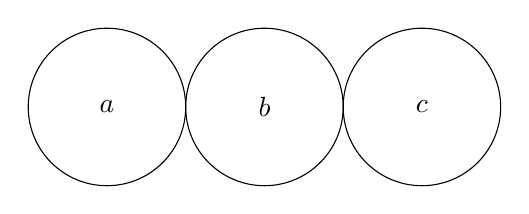
\begin{tikzpicture}
  \draw (0.0,0.0) circle (1cm);
  \draw (2.0,0.0) circle (1cm);
  \draw (4.0,0.0) circle (1cm);
  \node at (0.0,0.0) {$a$};
  \node at (2.0,0.0) {$b$};
  \node at (4.0,0.0) {$c$};
\end{tikzpicture}
\caption{Connectedness and transitivity}
\label{fig:connectedness-transitivity}
\end{figure} 

As discussed by \citet{casati_varzi1999parts}, there are a number of intuitive interactions between the topological notion $\cnst{c}$ and the mereological relations $\sqsubseteq$ and $\cnst{o}$. These intuitive interactions can be formalized as the so-called bridging principles which interrelate the mereological and the topological component of the theory (\citealt{varzi2007spatial}). The main aim of the bridging principles is to secure that, irrespective of their full characterization, $\sqsubseteq$ and $\cnst{c}$ are related in such a manner that a whole and its parts are firmly connected. In particular, the principle of \textsc{integrity} ensures that connectedness is implied by parthood, see \ref{ex:integrity}, and consequently mereological overlap is in fact a form of connection, as guaranteed by the principle of \textsc{unity}, see \ref{ex:unity}. Finally, the principle defined in \ref{ex:monotonicity} secures \textsc{monotonicity}.\footnote{In fact, \ref{ex:monotonicity} implies both \ref{ex:integrity} and \ref{ex:unity} \citep[pp. 981--982]{varzi2007spatial}. However, I provide all the bridging principles for the sake of completeness.}

	\ex. Integrity \citep[p. 981; adapted]{varzi2007spatial}\label{ex:integrity}\\
    $\forall x\forall y[x \sqsubseteq y \rightarrow \cnst{c}(x,y)]$\\
(If an m-individual is part of another m-individual, then they are connected.)

\ex. Unity \citep[p. 981; adapted]{varzi2007spatial}\label{ex:unity}\\
$\forall x\forall y[\cnst{o}(x,y) \rightarrow \cnst{c}(x,y)]$\\
(If two m-individuals overlap, then they are connected.)

\ex. Monotonicity \citep[p. 981; adapted]{varzi2007spatial}\label{ex:monotonicity}\\
$\forall x\forall y\big[x \sqsubseteq y \rightarrow \forall z [\cnst{c}(z,x) \rightarrow \cnst{c}(z,y)]\big]$\\
(If an m-individual is part of another m-individual, then whatever is connected to the former, is also connected to the latter.)

Given these extensions, a number of mereotopological properties like \textsc{internal part} (\cnst{ip}), \textsc{internal overlap} (\cnst{io}), and \textsc{tangential overlap} (\cnst{to}) can be defined. Such notions enable us to draw subtle topological distinctions in order to account for different spatial configurations that entities may be in. For instance, the individual $b$ in \figref{fig:internal-part} is an internal part of the individual $a$ since every entity that is connected to $b$ overlaps with $a$ or, in other words, $a$ includes $b$. On the other hand, though part of $b$ is an internal part of $a$ in \figref{fig:internal-overlap}, there is also a part of $b$ which is not included in $a$. Finally, \figref{fig:tangential-overlap} illustrates a configuration where there is overlap between $a$ and $b$ but there is no internal overlap, i.e., the individuals only share their edges.

\begin{figure}[h!]
\begin{floatrow}
\captionsetup{margin=.05\linewidth}
\ffigbox[.33\textwidth]{\caption{Internal part}\label{fig:internal-part}}
        {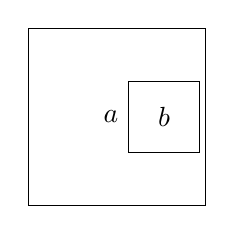
\begin{tikzpicture}[scale=.75]
           \node at (1.4,1.5) {$a$};
           \node at (2.3,1.5) {$b$};
           \draw (0,0) -- (0,3) -- (3,3) -- (3,0) -- (0,0);
           \draw (1.7,2.1) -- (2.9,2.1) -- (2.9,0.9) -- (1.7,0.9) -- (1.7,2.1);
         \end{tikzpicture}}
\ffigbox[.33\textwidth]{\caption{Internal overlap}\label{fig:internal-overlap}}
         {\begin{tikzpicture}[scale=.75]
           \node at (1.5,1.5) {$a$};
           \node at (3.3,1.5) {$b$};
           \draw (0,0) -- (0,3) -- (3,3) -- (3,0) -- (0,0);
           \draw (2.7,2.1) -- (3.9,2.1) -- (3.9,0.9) -- (2.7,0.9) -- (2.7,2.1);
         \end{tikzpicture}}
\ffigbox[.33\textwidth]{\caption{Tangential overlap}\label{fig:tangential-overlap}}
        {\begin{tikzpicture}[scale=.75]
         \node at (1.5,1.5) {$a$};
         \node at (3.6,1.5) {$b$};
         \draw (0,0) -- (0,3) -- (3,3) -- (3,0) -- (0,0);
         \draw (3,2.1) -- (4.2,2.1) -- (4.2,0.9) -- (3,0.9) -- (3,2.1);
         \end{tikzpicture}}
\end{floatrow}
\end{figure}

The relevant definitions are given in \ref{ex:internal-part}--\ref{ex:tangential-overlap}.

\ex. Internal part \citep[p. 55; adapted]{casati_varzi1999parts}\label{ex:internal-part}\\
$\cnst{ip}(x,y) \eqdef x \sqsubseteq y \wedge \forall z[\cnst{c}(z,x) \rightarrow \cnst{o}(z,y)]$

\ex. Internal overlap \citep[p. 55; adapted]{casati_varzi1999parts}\label{ex:internal-overlap}\\
$\cnst{io}(x,y) \eqdef \exists z[\cnst{ip}(z,x) \wedge \cnst{ip}(z,y)]$

\ex. Tangential overlap \citep[p. 55; adapted]{casati_varzi1999parts}\label{ex:tangential-overlap}\\
$\cnst{to}(x,y) \eqdef \cnst{o}(x,y) \wedge \neg \cnst{io}(x,y)$

In addition, within the mereotopological framework standard topological notions can be defined. Assuming \textsc{mereological complement} (${\sim}$), as provided in \ref{ex:mereological-complement}, \ref{ex:interior}--\ref{ex:boundary} give definitions for \textsc{interior} (\cnst{int}), \textsc{exterior} (\cnst{ext}), \textsc{closure} (\cnst{clo}), and \textsc{boundary} (\cnst{b}), respectively.   

\ex. Mereological complement\label{ex:mereological-complement} \citep[p. 45; adapted]{casati_varzi1999parts}\\
${\sim}(x) \eqdef \iota y\forall z[z \sqsubseteq y \leftrightarrow \neg\cnst{o}(z,x)]$

\ex. Interior\label{ex:interior} \citep[p. 58; adapted]{casati_varzi1999parts}\\
$\cnst{int}(x) \eqdef \sqcup X$ where $X = \{y\ :\ \cnst{ip}(y,x) = \cnst{true}\}$

\ex. Exterior\label{ex:exterior} \citep[p. 58; adapted]{casati_varzi1999parts}\\
$\cnst{ext}(x) \eqdef \cnst{int}({ \sim} (x))$

\ex. Closure\label{ex:closure} \citep[p. 58; adapted]{casati_varzi1999parts}\\
$\cnst{clo}(x) \eqdef { \sim}(\cnst{ext}(x))$

\ex. Boundary\label{ex:boundary} \citep[p. 58; adapted]{casati_varzi1999parts}\\
$\cnst{b}(x) \eqdef { \sim}(\cnst{int}(x) \sqcup \cnst{ext}(x))$

\figref{fig:interior}--\ref{fig:closure} illustrate the intended configurations.

\begin{figure}
\begin{floatrow}
  \captionsetup{margin=.05\linewidth}
  \ffigbox[.33\textwidth]{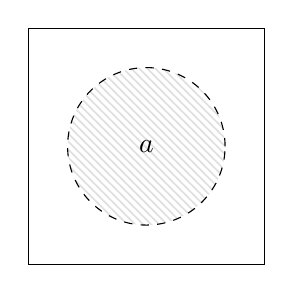
\begin{tikzpicture}
  \draw (0,0) -- (0,3) -- (3,3) -- (3,0) -- (0,0);
  \draw[dashed,pattern=south east lines,pattern color=gray!25] (1.5,1.5) circle (1cm);
  \node at (1.5,1.5) {$a$};
  \end{tikzpicture}}
  {\caption{Interior\label{fig:interior}}}
  \ffigbox[.33\textwidth]{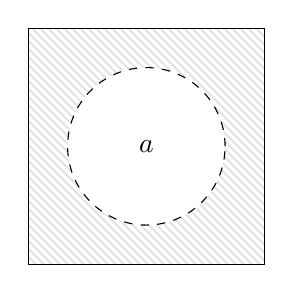
\begin{tikzpicture}
  \draw[pattern=south east lines,pattern color=gray!25] (0,0) -- (0,3) -- (3,3) -- (3,0) -- (0,0);
  \draw[dashed,fill=white] (1.5,1.5) circle (1cm);
  \node at (1.5,1.5) {$a$};
   \end{tikzpicture}}
   {\caption{Exterior\label{fig:exterior}}}
  \ffigbox[.33\textwidth]{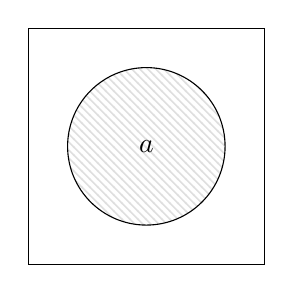
\begin{tikzpicture}
  \draw (0,0) -- (0,3) -- (3,3) -- (3,0) -- (0,0);
  \draw[pattern=south east lines,pattern color=gray!25] (1.5,1.5) circle (1cm);
  \node at (1.5,1.5) {$a$};
  \end{tikzpicture}}
  {\caption{Closure\label{fig:closure}}}
\end{floatrow}
\end{figure}

\iffalse

\begin{figure}[h!]
\RawFloats
\centering
\begin{minipage}[b]{.49\textwidth}
\centering
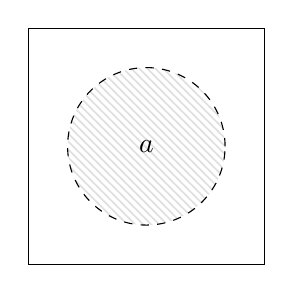
\begin{tikzpicture}
  \draw (0,0) -- (0,3) -- (3,3) -- (3,0) -- (0,0);
  \draw[dashed,pattern=south east lines,pattern color=gray!25] (1.5,1.5) circle (1cm);
  \node at (1.5,1.5) {$a$};
\end{tikzpicture}
\caption{Interior}
\label{fig:interior}
\end{minipage}
\begin{minipage}[b]{.49\textwidth}
\centering
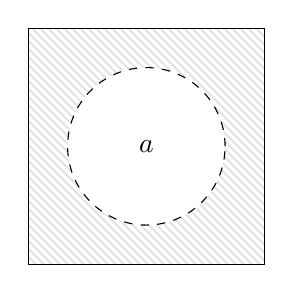
\begin{tikzpicture}
  \draw[pattern=south east lines,pattern color=gray!25] (0,0) -- (0,3) -- (3,3) -- (3,0) -- (0,0);
  \draw[dashed,fill=white] (1.5,1.5) circle (1cm);
  \node at (1.5,1.5) {$a$};
\end{tikzpicture}
\caption{Exterior}
\label{fig:exterior}
\end{minipage}
~
\begin{minipage}[b]{1.0\textwidth}
\vspace{1.0ex}
\centering
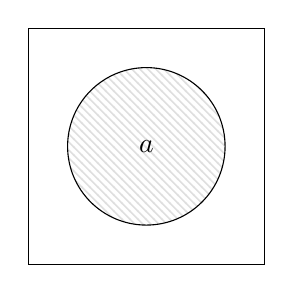
\begin{tikzpicture}
  \draw (0,0) -- (0,3) -- (3,3) -- (3,0) -- (0,0);
  \draw[pattern=south east lines,pattern color=gray!25] (1.5,1.5) circle (1cm);
  \node at (1.5,1.5) {$a$};
\end{tikzpicture}
\caption{Closure}
\label{fig:closure}
\end{minipage}
\end{figure}

\fi

The shaded area in \figref{fig:interior} represents the interior of an object, which is taken to be the sum of an m-individual's internal parts. The dashed line marks the boundary of the object, i.e., the part that is not included in its interior. On the other hand, \figref{fig:exterior} represents the exterior of an object, which again does not comprise the boundary, whereas the solid line in \figref{fig:closure} indicates that both the interior and boundary make up the closure of an entity.

The framework described so far extends standard mereology with the primitive topological relation of connectedness and several derived notions, which allow us to talk about different configurations that entities can be in. Such a system provides means to distinguish between arbitrary and non-arbitrary sums, and consequently to define individuals as integrated wholes, i.e., objects characterized in terms of different degrees of connectedness. The following section will discuss a mereotopological approach to such individuals.

\subsection{Integrated wholes}\label{sec:integrated-wholes}

A great advantage of the mereotopological approach to natural language semantics is that by means of the topological relations defined so far it is possible to capture what it means to be an individual understood as an integrated whole. In particular, a distinction can be drawn between entities which come in one piece, as opposed to pluralities, i.e., scattered entities, which bear no topological commitments. To distinguish the former from the latter, it is essential to introduce the property \textsc{self-connected} (\cnst{sc}). Unlike arbitrary sums, \cnst{sc} entities cannot be divided into separated parts. The definition of \cnst{sc} is provided in \ref{ex:self-connected}.
	
	\ex. Self-connected \citep[p. 57; adapted]{casati_varzi1999parts}\label{ex:self-connected}\\
    $\cnst{sc}(x) \eqdef \forall y \forall z[\forall w(\cnst{o}(w,x) \leftrightarrow (\cnst{o}(w,y) \vee \cnst{o}(w,z))) \rightarrow \cnst{c}(y,z)]$\\
	(An entity is self-connected if and only if any two parts that form the whole of that entity are connected to each other.)
	
    Given the definition in \ref{ex:self-connected}, it is possible to differentiate inseparable individuals from separable ones including arbitrary sums of entities, i.e., disconnected configurations of objects. To illustrate this let us assume a model containing four entities. Specifically, suppose $a$ and $b$ are two halves of a cube, whereas $c$ and $d$ are a pyramid and a sphere, respectively, see \figref{fig:wholes-sums}. Intuitively, there is a difference between the sum $s_1 = a \sqcup b$ and the sum $s_2 = c \sqcup d$. While $s_1$ forms an integrated whole, the plurality $s_2$ is just an arbitrary collection of disconnected objects, and thus it does not make up a solid whole. In other words, $\cnst{sc}(s_1)$ is true, whereas $\cnst{sc}(s_2)$ is false. 
    
\begin{figure}[h!]
\centering
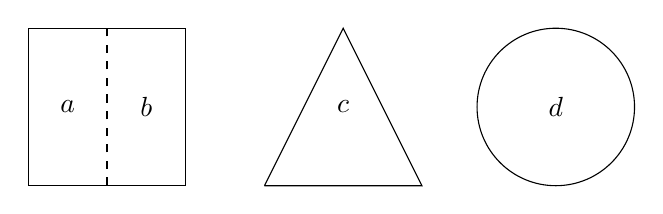
\begin{tikzpicture}
  \draw (0,0) -- (2,0) -- (2,2) -- (0,2) -- (0,0);
  \draw[dashed] (1,0) -- (1,2);
  \draw (3,0) -- (4,2) -- (5,0) -- (3,0);
  \draw (6.7,1) circle (1cm);
  \node at (0.5,1) {$a$};
  \node at (1.5,1) {$b$};
  \node at (4,1) {$c$};
  \node at (6.7,1) {$d$};  
\end{tikzpicture}
\caption{Wholes vs. sums}
\label{fig:wholes-sums}
\end{figure}      
    
    Self-connectedness is a great improvement in the theory of wholeness. However, this notion is still insufficient to capture what it means to be conceptualized as an integrated object since it allows for configurations involving only an external connection holding between individuals. In other words, cases when the closure of one object overlaps the other or vice versa are not ruled out. For instance, \figref{fig:external-connection} depicts two spheres $a$ and $b$ which only touch each other, i.e., their boundaries are connected at a single point. Given the definition of \cnst{sc} in \ref{ex:self-connected}, $a$ and $b$ are self-connected but intuitively such a spatial configuration is not sufficient to count as an integrated whole.
    
\begin{figure}[h!]
\centering
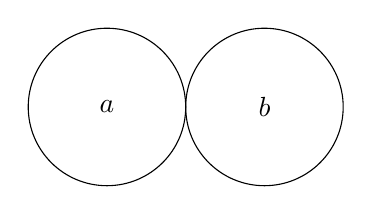
\begin{tikzpicture}
  \draw (0.0,0.0) circle (1cm);
  \draw (2.0,0.0) circle (1cm);
  \node at (0.0,0.0) {$a$};
  \node at (2.0,0.0) {$b$};
\end{tikzpicture}
\caption{External connection}
\label{fig:external-connection}
\end{figure}    
  
In order to rule out cases such as the one illustrated in \figref{fig:external-connection}, a stronger relation is required. Ostensibly, what is necessary is that not only boundaries of parts of a whole are connected to each other, but also that their internal parts are shared. To solve this problem one needs to define an additional restriction on the concept of interior given in \ref{ex:interior}. Accordingly, \citet{casati_varzi1999parts} postulate the property of being \textsc{strongly self-connected} (\cnst{ssc}), as defined in \ref{ex:strongly-self-connected}.\footnote{Notice that on some plausible assumptions concerning boundaries the first conjunct in \ref{ex:strongly-self-connected} is superfluous (for a discussion of various views on boundaries, see \citealt[pp. 61--62, 71--98]{casati_varzi1999parts}).} This refinement will get us much closer to the type of entities we would like to single out, i.e., integrated wholes.

	\ex. Strongly self-connected \citep[p. 60; adapted]{casati_varzi1999parts}\label{ex:strongly-self-connected}\\
    $\cnst{ssc}(x) \eqdef \cnst{sc}(x) \wedge \cnst{sc}(\cnst{int}(x))$\\
    (An m-individual is strongly self-connected if it is self-connected and its interior is self-connected.)
	
	The restriction introduced in \ref{ex:strongly-self-connected} guarantees that not only boundaries of parts are shared but also that the interior of an entity is self-connected. Therefore, the property of \cnst{ssc} rules out objects that merely touch each other, e.g., the spheres in \figref{fig:external-connection}. However, the fact that an entity is strongly self-connected still does not ensure that such an entity is an integrated whole in the sense a theory of wholeness is supposed to capture. For instance, consider the entity $a$, i.e., the left half of the cuboid represented in \figref{fig:strongly-self-connected-part}. Although $a$ qualifies as a strongly self-connected object since any two parts that form its interior are connected, intuitively it cannot be characterized as a whole. Obviously, the reason is that there is yet another half of the cuboid and only the two together make up the entire individual. Consequently, \cnst{ssc} is insufficient for our purposes and an even stronger notion is required to capture what is perceived as an integral whole.

\begin{figure}[h!]
\centering
\begin{tikzpicture}
  \draw (0,0) -- (2,0) -- (2,2) -- (0,2) -- (0,0);
  \draw[dashed] (1,0) -- (1,2);
  \node at (0.5,1) {$a$};
\end{tikzpicture}
\caption{Strongly self-connected part}
\label{fig:strongly-self-connected-part}
\end{figure}

	Describing wholes is about capturing an intuitive notion of unity. This means that a proper definition should accommodate both topological integrity and mereological exhaustivity. For this purpose, \citet{casati_varzi1999parts} introduce the property of being \textsc{maximally strongly self-connected} (\cnst{mssc}), as defined in \ref{ex:maximally-strongly-self-connected}.
	
	\ex. Maximally-strongly-self-connected \citep[p. 60; adapted]{casati_varzi1999parts}\label{ex:maximally-strongly-self-connected}\\
	$\cnst{mssc}(x) \eqdef \cnst{ssc}(x) \wedge \forall y[\cnst{ssc}(y) \wedge \cnst{o}(y,x) \rightarrow y \sqsubseteq x]$\\
    (An m-individual is maximally strongly self-connected if (i)~every part of the individual is connected to (overlaps) the whole (strongly self-connect\-ed) and (ii)~anything else which overlaps it and is strongly self-connected is once again part of it (maximality).)

	More generally one could single out entities that are maximally strongly self-connected relative to a particular property. The relativized \cnst{mssc} property can be characterized as in \ref{ex:maximally-strongly-self-connected-relative}, which provides the final mereotopological definition of what an integrated whole is.
	
	\ex. Maximally strongly self-connected relative to a property \citep[p. 60; adapted]{casati_varzi1999parts}\label{ex:maximally-strongly-self-connected-relative}\\
	$\cnst{mssc}(P)(x) \eqdef P(x) \wedge \cnst{ssc}(x) \wedge \forall y[P(y) \wedge \cnst{ssc}(y) \wedge \cnst{o}(y,x) \rightarrow y \sqsubseteq x]$\\
     (An m-individual is maximally strongly self-connected relative to a property if (i) every part of the individual is connected to (overlaps) the whole (strongly self-connected) and (ii) anything else which has the same property, is strongly self-connected, and overlaps it is once again part of it (maximality).)
	
	If an entity satisfies \cnst{mssc}, then it is the largest entity satisfying that property which is self-connected. For instance, if $P$ is the property of being a cuboid, then the definition in \ref{ex:maximally-strongly-self-connected-relative} will select the largest such entities among those that come in one piece. In particular, it will single out the whole cuboid in \figref{fig:strongly-self-connected-part} as opposed to, e.g., its left half $a$ though $a$ itself also satisfies the property of being a cuboid. That is because $a$ is part of the cuboid whereas the whole cuboid is not part of any other strongly self-connected object.
    
    Though the structure of the mereotopological framework of \citet{casati_varzi1999parts} discussed above is relatively simple, the distinctions developed within it are fine-grained enough for the representation of spatial objects. As standard mereology, mereotopology gives rise to algebraic structures isomorphic to \linebreak Boolean algebras with their bottom element removed. However, such lattice representations are further endowed with regions indicating which elements are associated with the connectedness relation \cnst{c}. For instance, consider \figref{fig:parthood-and-connectedness}. 
     
    \begin{figure}[h!]
\centering
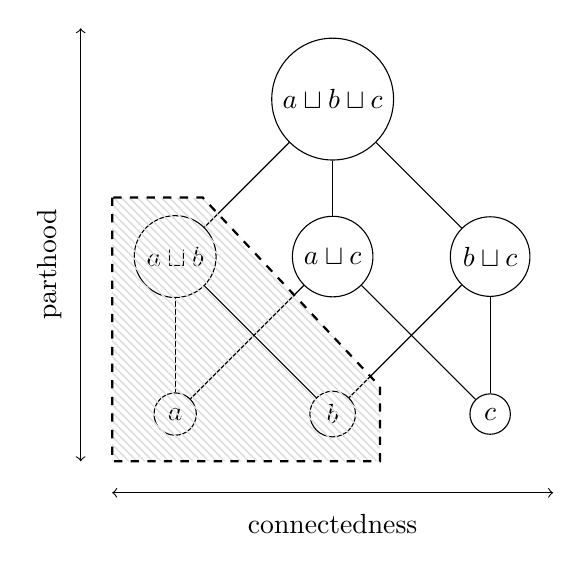
\begin{tikzpicture}[node distance=2cm]
  \node[draw=black,thin,circle,inner sep=3pt] (abc) {$a \sqcup b \sqcup c$};
  \node[draw=black,thin,circle,inner sep=3pt] (ac) [below of=abc] {$a \sqcup c$};
  \node[draw=black,thin,circle,inner sep=3pt] (ab) [left of=ac] {$a \sqcup b$};
  \node[draw=black,thin,circle,inner sep=3pt] (bc) [right of=ac] {$b \sqcup c$};
  \node[draw=black,thin,circle,inner sep=3pt] (a) [below of=ab] {$a$};
  \node[draw=black,thin,circle,inner sep=3pt] (b) [right of=a] {$b$};
  \node[draw=black,thin,circle,inner sep=3pt] (c) [right of=b] {$c$};
  \draw (a) -- (ab);
  \draw (a) -- (ac);
  \draw (b) -- (ab);
  \draw (b) -- (bc);
  \draw (c) -- (ac);
  \draw (c) -- (bc);
  \draw (ab) -- (abc);
  \draw (ac) -- (abc);
  \draw (bc) -- (abc);
  \draw[thick,dashed,pattern=south east lines,pattern color=gray!25] (-2.8,-1.25) -- (-2.8,-4.6) -- (0.6,-4.6) -- (0.6,-3.65) -- (-1.65,-1.25) -- (-2.8,-1.25); 
  \draw[<->] (-3.2,0.9) -- (-3.2,-4.6);
  \draw[<->] (-2.8,-5.0) -- (2.8,-5.0);
  \node at (0.0,-5.4) {connectedness};
  \node[rotate=90] at (-3.6,-2.1) {parthood};
\end{tikzpicture}
\caption{Parthood and connectedness \citep[based on][p. 136]{grimm2012number}}
\label{fig:parthood-and-connectedness}
\end{figure}

Given a model with 3 entities, namely two halves of a cube $a$ and $b$ and a pyramid $c$, the semi-lattice represents all the possible sums generated by the set of corresponding m-individuals. The vertical axis illustrates the parthood relation with individual lines between particular nodes symbolizing $\sqsubseteq$, whereas the horizontal axis represents connectedness. The shaded area then covers those entities in the structure which are connected. In other words, the mereological component of the theory defines part-whole relations between $a$, $b$, and $c$ and all the possible sums thereof, whereas the topological component singles out those parts that form self-connected wholes. In particular, while $a$ in the model is part of $a \sqcup b$ (as well as of itself due to the axiom of reflexivity), it is not part of $b$. However, it is connected to $b$ (as well as to $a \sqcup b$ due the axiom of integrity and to itself -- again reflexivity).
   
    Moreover, as discussed by \citet{grimm2012number}, the subtle niceties between different types of connectedness provide means to capture differences between distinct types of nominals, such as object, substance, and aggregate nouns, as well as eliminate old problems concerning cumulative singular count nouns such as \textit{fence} or \textit{twig} \citep[see, e.g.,][]{zucchi_white2001twigs,rothstein2010counting}. Specifically, among multiple parts that have a property of being, say, a rock only the maximal (improper) part counts as a whole object. Hence, I conclude that compared to standard mereology, mereotopology proves to be a superior theory of parts and wholes and its application in natural language semantics should be considered advantageous. In the next section I will discuss several other kinds of connection. 

\subsection{Other types of connection}\label{sec:other-types-of-connection}

In the previous section, we saw that given the primitive relation \cnst{c} it is possible to derive a notion that can capture what it means to be an integrated whole as opposed to an arbitrary sum, namely the \cnst{mssc} property. This, however, does not deplete the potential of mereotopology in modeling different types of objects and spatial configurations. Based on \cnst{c}, many other types of topological relations representing distinct varieties of connectedness may be defined. In this section, I will discuss some of them.

\begin{sloppypar}
The first auxiliary mode of connection to be discussed is the property of \textsc{firmly connected} (\cnst{fc}), as defined in \ref{ex:firmly-connected}.\footnote{I use the term following \citet{varzi2007spatial}, whereas \citet{casati_varzi1999parts} and \citet{grimm2012degrees,grimm2012number} talk about strong connection. My motivation is mainly to avoid potential confusion with the \cnst{ssc} property which plays a crucial role in defining \cnst{fc} but is distinct from it.} 
\end{sloppypar}

\ex. Firmly connected \citep[p. 1003; adapted]{varzi2007spatial}\label{ex:firmly-connected}\\
$\cnst{fc}(x,y) \eqdef \exists w \exists z[w \sqsubseteq x \wedge z \sqsubseteq y \wedge \cnst{ssc}(w \sqcup z)]$\\
(Two m-individuals are firmly connected if a sum of their parts is strongly self-connected.)

This property holds between two entities when they overlap in a substantive sense. In other words, two m-individuals are firmly connected if their sum is strongly self-connected. Such a definition excludes cases of tangential overlap, i.e., configurations where entities only touch each other, since the \cnst{ssc} property implies that not only the boundaries but also the interiors of m-individuals are connected.

With an additional restriction regarding the local scope of connectedness, the notion of \cnst{fc} seems to be suitable to capture what it means to be conceptualized as a substance, as opposed to an integrated individual that we count as one. Specifically, substances can be represented as comprising of m-individuals that are locally firmly connected, i.e., at a given location an instance of a substance is always firmly connected to another instance of the same substance \citep[pp. 140--142]{grimm2012degrees,grimm2012number}. For instance, a section of mud in a puddle overlaps with other sections of the puddle of mud, which are again mud.  

In contrast to \cnst{fc}, the property \textsc{externally connected} (\cnst{ec}), as defined in \ref{ex:externally-connected}, concerns entities that are merely tangentially connected, i.e., it is only their boundaries that are connected, whereas their interiors do not overlap. This notion enables us to model configurations of entities that are not merged but simply touch each other.

\ex. Externally connected \citep[p. 134; adapted]{grimm2012number}\label{ex:externally-connected}\\
$\cnst{ec}(x,y) \eqdef \cnst{c}(x,y) \wedge \neg \cnst{c}(\cnst{int}(x),\cnst{int}(y))$\\
(Two m-individuals are externally connected if they are connected but it is not the case that their interiors are connected.)

Another topological notion it might be useful to derive is one describing a configuration of objects touching each other in such a way that they form, say, a row. This variety of connectedness can be captured by the property \textsc{by-connected} (\cnst{bc}), as provided by \citet{varzi2007spatial}. It holds between entities that are not connected to each other but are associated by virtue of being connected to another mediating entity. The definition in \ref{ex:by-connected} describes \cnst{bc} as a three-place relation establishing indirect connectedness between the outermost entities within a configuration.

\ex. By-connected \citep[p. 979; adapted]{varzi2007spatial}\label{ex:by-connected}\\
$\cnst{bc}(x,y,z) \eqdef \cnst{c}(x,z) \wedge \cnst{c}(z,y)$\\
(Three m-individuals $x$, $y$, and $z$ are by-connected if $x$ is connected to $z$ and $z$ is connected to $y$.)

A related notion is called \textsc{mediately connected} (\cnst{mc}). This is a binary relation that holds between entities that are not necessarily connected to each other, but are part of a by-connected configuration, e.g, a row of individuals. In other words, there is an object that mediates the connection between two such entities. The formal definition of \cnst{mc} is given in \ref{ex:mediately-connected}.

\ex. Mediately connected \citep[p. 979; adapted]{varzi2007spatial}\label{ex:mediately-connected}\\
$\cnst{mc}(x,y) \eqdef \exists z [\cnst{bc}(x,y,z)]$\\
(Two m-individuals are mediately connected if they are by-connected through a third m-individual.)

\pagebreak To illustrate the \cnst{bc} and \cnst{mc} relations, consider the configuration of two spheres $a$ and $c$ and a cube $b$, as depicted in  \figref{fig:by-connected-and-mediately-connected}. The three entities are by-connected since $a$ is externally connected to $b$ and $b$ is externally connected to $c$. At the same time, the spheres are mediately connected since both $a$ and $c$ are connected to the cube $b$, i.e., $b$ in a way mediates the connection between $a$ and $c$.

\begin{figure}[h!]
\centering
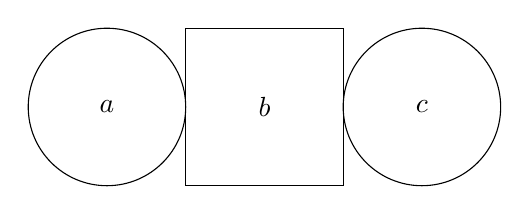
\begin{tikzpicture}
  \draw (0.0,0.0) circle (1cm);
  \draw (1.0,-1.0) -- (3.0,-1.0) -- (3.0,1.0) -- (1.0,1.0) -- (1.0,-1.0);
 \draw (4.0,0.0) circle (1cm);
  \node at (0.0,0.0) {$a$};
  \node at (2.0,0.0) {$b$};
  \node at (4.0,0.0) {$c$};
\end{tikzpicture}
\caption{By-connected and mediately connected}
\label{fig:by-connected-and-mediately-connected}
\end{figure}

As pointed out by \citet[pp. 134--135]{grimm2012number}, the notion of \cnst{mc} may prove useful in modeling natural language expressions denoting entities such as eyes or fingers. Such objects seem to be conceptualized in a particular way which is further reflected in grammar. Specifically, in some languages they belong to a category of inherently plural or dual expressions.

Furthermore, the \cnst{bc} relation can be generalized to hold for any number of entities. This gives rise to the property \textsc{transitively connected} (\cnst{tc}). As defined in \ref{ex:transitively-connected} \citep[see][p. 144]{grimm2012degrees,grimm2012number}, it is intended to determine whether two individuals are connected through a series of mediating entities. For instance, it would hold of two opposite entities in a scenario similar to the one illustrated in  \figref{fig:by-connected-and-mediately-connected} with the exception that between the spheres $a$ and $c$ there is not only the cube $b$, but also a pyramid $d$ such that it touches both $b$ an $c$.

\ex. Transitively connected \citep[p. 15; adapted]{grimm2012degrees}\label{ex:transitively-connected}\\
$\cnst{tc}(x,y,P,C,Z) \eqdef \forall z \in Z[P(z) \wedge (x = z_1 \wedge y = z_n) \wedge Cz_1z_2 \wedge Cz_2z_3 \dots \wedge Cz_{n-1}z_n]$\\
where $Z = \{z_1,z_2,\dots z_n\}$\\
(Entities $x$ and $y$ are transitively connected relative to a property $P$, a connection relation $C$, and a set of entities $Z$, when all members of $Z$ satisfy $P$ and $x$ and $y$ are connected through the sequence of $z_i$s in $Z$.)

The property \cnst{tc} allows for defining the concept of \textsc{cluster} (\cnst{clstr}) \citep[see][p. 144]{grimm2012degrees,grimm2012number}. According to \ref{ex:cluster}, a cluster is a special type of entity that is conceptualized as a plurality of m-individuals that are transitively connected, i.e., they compose a connected sequence. For instance, the sum $a\sqcup b\sqcup c$ in \figref{fig:by-connected-and-mediately-connected} forms a cluster relative to the property of being a three-dimensional geometrical object.

	\ex. Cluster \citep[p. 144; adapted]{grimm2012number}\\
	$\cnst{clstr}(x,P,C) \eqdef \exists Z[x = \bigsqcup Z \wedge \forall z \forall z' \in Z \exists Y[\cnst{tc}(z,z',P,C,Y)]]$\\
	(An entity $x$ is a cluster relative to a property $P$ and a connection relation $C$ iff $x$ is a sum of entities falling under the same property which are all transitively connected relative to some set $Y$ under the same property and connection relation.)\label{ex:cluster}

Though the notions of \cnst{tc} and \cnst{clstr} are intriguing and important mereotopological concepts, the definitions in \ref{ex:transitively-connected} and \ref{ex:cluster} seem to give rise to certain unintended consequences.\footnote{I would like to sincerely thank Nina Haslinger for pointing this out as well as suggesting a solution.} In \ref{ex:transitively-connected}, the argument $Z$ being a set does not have an inherent ordering. However, the indexed variables $z_1,z_2,\dots z_n$ make reference to some ordering of this set. Since there is no quantifier over these variables in \ref{ex:transitively-connected}, the particular indexing assumed for a given case in fact determines whether the relation $\cnst{tc}(x,y,P,C,Z)$ holds or not. For instance, if $Z = \{a,b,c\}$ such that $a$ and $b$ are connected, $b$ and $c$ are connected and no other connections hold, the condition in \ref{ex:transitively-connected} is met for $z_1 = a$, $z_2 = b$, $z_3 = c$ but not for $z_1 = a$, $z_2 = c$, $z_3 = b$. This seems counterintuitive since, given the context of \citet{grimm2012degrees,grimm2012number}, the intention behind \ref{ex:transitively-connected} must be that it is valid whenever there is \textit{some} finite sequence $\langle z_1, \dots, z_n\rangle$ such that $Z = \{z_1, \dots, z_n\}$, $x=z_1$, $y=z_n$ and for every index $i$, such that $1 \leq i < n$, the connection relation $C(z_i, z_{i+1})$ holds. And yet, based on \ref{ex:transitively-connected}, it seems like some particular such sequence must be always contextually given, which means it is unclear how to apply \ref{ex:transitively-connected} in the context of \ref{ex:cluster}.

Another problem is that the definition of a cluster in \ref{ex:cluster} has the following counterintuitive consequence. Let $P = \{z1, z2, z3\}$ and $Z = \{z1, z3\}$ and assume that $z_1$ and $z_2$ are connected, $z_2$ and $z_3$ are connected and nothing else is connected. In such a case, $z_1$ and $z_3$ are transitively connected via the set $Y = \{z_1, z_2, z_3\}$, which is a subset of $P$, so the sum $z1 \sqcup z3$ should form a cluster relative to $P$ and $C$, even though it is not a connected entity.

In order to avoid the problems discussed above, I propose the revised definitions for \cnst{tc} and \cnst{clstr} in \ref{ex:transitively-connected-new} and \ref{ex:cluster-new}, respectively. The main difference between \ref{ex:transitively-connected} and \ref{ex:transitively-connected-new} is that in the revised version the quantification over possible orderings of $Z$ is made explicit, i.e., the parameter $Z$ ranges over sequences rather than unordered sets.\largerpage[2]

\ex. Transitively connected (revised)\\
$\cnst{tc}(x,y,P,C,Z) \eqdef z_1 = x \wedge z_n = y \wedge \forall i[1 \leq i < n \rightarrow C(z_i,z_{i+1})]\\
\wedge \forall i[1 \leq i \leq n \rightarrow P(z_i)]$, where $Z = \langle z_1, \dots, z_n\rangle$\\
(Entities $x$ and $y$ are transitively connected relative to a property $P$, a connection relation $C$, and a finite sequence of entities $Z$, when all members of $Z$ satisfy $P$ and $x$ and $y$ are connected through the sequence of $z_i$s in $Z$.)\label{ex:transitively-connected-new}

Furthermore, the key modification in \ref{ex:cluster-new}, as compared to \ref{ex:cluster}, is that in \ref{ex:cluster-new} the variable $Y$ is restricted to the subsets of $Z$. This excludes configurations such as the unconnected sum $z1 \sqcup z3$ in the scenario discussed above. 

\ex. Cluster (revised)\\
$\cnst{clstr}(x,P,C) \eqdef \exists Z[x = \bigsqcup Z \wedge \forall z \forall z' \in Z \exists Y \subseteq Z[\cnst{tc}(z,z',P,C,Y)]]$\\
(An entity $x$ is a cluster relative to a property $P$ and a connection relation $C$ iff $x$ is a sum of entities falling under the same property which are all transitively connected relative to $Y$ which is a subset of a sequence $Z$ under the same property and connection relation.)\label{ex:cluster-new}

Finally, the weakest variety of connectedness can be captured by the notion of \textsc{proximately connected} (\cnst{pc}).\footnote{In order to refer to a similar concept, \citet{casati_varzi1999parts} use the term quasi-connected. However, I will follow \citeposst{grimm2012number} terminology and formalism here.} This relation concerns entities that are neither contiguous, nor do they touch each other, but rather they are ``very close''. The formula in \ref{ex:proximately-connected} defines \cnst{pc} in terms of the distance function \cnst{d} which yields the distance between two entities it is applied to. For instance, if a sphere $a$ is 1 meter away from a cube $b$, the distance function \cnst{d} would yield 1 meter. The value $n$ is determined with respect to the predicate in question so that entities that satisfy it are conceptualized as being sufficiently near each other relative to the relevant property.

\ex. Proximately connected \citep[p. 135; adapted]{grimm2012number}\label{ex:proximately-connected}\\
$\cnst{pc}(x,y,P) \eqdef \cnst{d}(x,y) \leq n(P)$\\
(Two m-individuals are proximately connected if the distance between them is lesser than or equal to the value determined for a given predicate.)

The overview provided here does not by any means exhaust possible configurations of objects and different types of connectedness. Nonetheless, for our purposes the notions introduced in this section will be absolutely sufficient. The introduced distinctions allow us to differentiate between several types of entities. First, due to the \cnst{mssc} relation it is possible to distinguish between arbitrary sums and solid integrated wholes. On the other hand, the \cnst{fc} property might be useful in capturing the nature of substances, i.e., entities that come in multiple instances which overlap each other. Furthermore, the \cnst{tc} relation enables us to single out entities consisting of connected objects arranged in configurations such as rows and piles, whereas \cnst{pc} provides means to describe entities involving multiple parts remaining in a proximate distance from each other such as complex mechanical devices as well as swarms \citep[see, e.g., ][]{henderson2017swarms}.

\section{Summary}\label{sec:summary-ch6}

In this chapter, I presented a theory of parts and wholes called mereotopology. The described system involves a mereological core devised to capture the intuitive notion of parthood. This allows us to relate elements that are part of certain larger entities with those entities. However, what standard mereology cannot account for are certain relations between parts that result in different spatial configurations. This is where the topological component introduces the notion of connectedness. Based on this primitive concept more sophisticated properties can be derived. From the perspective of this study, the most prominent is the property of being a maximally strongly self-connected individual. This notion enables us to capture integrated wholes, i.e., objects that are conceptualized as coming in one piece. In the next chapter, I will demonstrate how the mereotopological framework introduced here can be used to model individuals in term of integrated wholes as well as continuous fragments of such wholes as integrated parts. Such treatment will allow us to better understand countability and to develop a novel account for subatomic quantification.

	\chapter{Mereotopological account for subatomic quantification}\label{ch:mereotopological-account-for-subatomic-quantification}
	
	Given the mereotopological framework introduced in the previous chapter, let us now attempt to account for some of the relevant expressions employing quantification over parts such as partitives and multiplier phrases as discussed in Chapter \ref{ch:partitives-and-part-whole-structures}, \ref{ch:exploring-topological-sensitivity}, and \ref{ch:multipliers}. The conceptual basis of the general mechanism of subatomic quantification outlined in Chapter \ref{ch:conceptual-background} can now be spelled out formally with the notions of parthood and connectedness playing the central role in modeling the meaning of expressions that provide objects to be counted as well as of those that do the counting. 
	
	In this chapter, I will propose an analysis of different types of partitives and multiplier phrases. I will start with the general discussion of the implausibility of atomicity-based approaches to subatomic quantification. Next, I will turn to my own proposal spelled out in terms of mereotopology, supplemented with additional components such as measure functions, partitions, and the individuation operation. First, I will address the mass/count distinction by distinguishing between different types of nominals, as well as give the meaning of the plural in the spirit of \citet{grimm2012number}. Subsequently, I will turn to defining other semantic objects I assume in the structure of different types of partitives and multiplier phrases including the meanings of different types of partitive words as well as numerical expressions, which I treat as complex constituents comprising a classifier component. Finally, I will propose a compositional analysis of the expressions in question by showing how the pieces fit together.
	
	\section{Doing without atoms}\label{sec:doing-without-atoms}
	
	In standard theories of pluralities and countability the mass/count distinction is often formulated in terms of atomicity \citep[e.g.,][]{link1983logical,landman1991structures,landman2000events,chierchia1998plurality,chierchia2010mass}. Though particular theories differ significantly with respect to the exact character of the alternation, the contrast between count and mass nouns usually boils down to the existence or lack of minimal building blocks in their denotation or, alternatively, to a distinct nature of those building blocks. The approach developed here rejects the view that what counts as one is best represented as an atomic entity. Instead, I build on the mereotopological notion of \cnst{mssc} introduced in  \sectref{sec:integrated-wholes} to capture what can be an object of counting. There are three main motivations behind this decision. The first one is the linguistic relevance of topological relations holding between parts of a whole object as empirically attested in multiple constructions in various languages discussed in Chapters \ref{ch:partitives-and-part-whole-structures} and \ref{ch:exploring-topological-sensitivity}. The second stems from the general counting principles described in  \sectref{sec:general-counting-principles}, which I believe constitute a deeply rooted part of human cognition and as such interact with that part of the language faculty that generates the grammar of countability. Finally, the last reason for abandoning atomicity is simply that it does not seem helpful with respect to subatomic quantification. Before we move on to the proper proposal, let us briefly consider why that is.

	Things that count as one are typically defined as atomic individuals, i.e., entities that have no proper parts, see \ref{ex:atom} for the definition of the notion \textsc{atom} and \ref{ex:atomicity} for an optional mereological axiom of \textsc{atomicity} that delivers atomic domains, i.e., domains consisting of atoms.
	
	\ex. Atom\\
	$\cnst{atom}(x) \leftrightarrow \neg \exists y[y \sqsubset x]$\\
	(An atom is an entity which has no proper parts.)\label{ex:atom}
	
	\ex. Atomicity\\
	$\forall x \exists y[y \sqsubseteq x \wedge \neg \exists z[z \sqsubset y]]$\\
	(For any element, there is a part for which there does not exist a proper part.)\label{ex:atomicity}
	
	At first blush, such an approach to what it means to count as one seems counterintuitive since we know from our everyday life experience that things we count as one very often do have multiple parts. However, one should not confuse intuitive concepts with formal notions devised to represent the semantics of natural language expressions, e.g., the meaning of the English partitive word \textit{part} with $\sqsubseteq$. Thus, my view is that there is nothing wrong in dissociating intuitive entities from their intuitive parts in terms of mereological modeling as long as it serves a certain purpose. For instance, \citet{champollion2010parts,champollion2017parts} assumes that the relation between, say, a teddy bear named Fuzzy Wuzzy and its paw is not mereological parthood. In other words, despite the fact that Fuzzy Wuzzy consists of a number of material parts it is considered a mereological atom, i.e., an inseparable unit in the domain of entities. This might seem plausible since it corresponds to yet another intuition, namely that though we know that things have parts, we seem to ignore this fact when we count those things. However, a significant problem for such an account arises when we decide to quantify not over whole things but over parts of those things. Thus, I will argue for two claims. First, having a notion of atomicity is not enough for a full analysis of quantification of parts. Second, atomicity is actually not needed to analyze quantification over parts since it can be reduced to topological notions which are required independently.
	
	To illustrate this, let us consider the following case involving subatomic quantification. Assume we wanted to count parts of Fuzzy Wuzzy, e.g., its paws. Of course, natural language allows for that since we can say \ref{ex:fuzzy-wuzzy-part}.
	
	\ex. English (Peter Sutton, p.c.)\\
	Exactly two parts of Fuzzy Wuzzy are brown.\label{ex:fuzzy-wuzzy-part}

	The sentence in \ref{ex:fuzzy-wuzzy-part} would be true if, say, Fuzzy Wuzzy's paws were brown where\-as all of its other parts were of a different color. However, if referents of proper names are mereological atoms, there are no parts to be counted since the entity designated by the expression \textit{Fuzzy Wuzzy} cannot be split. Without saying anything else, this is untenable if we want to account for \ref{ex:fuzzy-wuzzy-part}. Consequently, one could follow \citet{link1983logical} and propose to distinguish between a domain of entities and a domain of portions of matter over which a different parthood relation would be defined, i.e., the material parthood relation $\sqsubseteq_m$ as opposed to the individual parthood relation $\sqsubseteq_i$. Assuming the domains are related by a function from entities to portions of matter, one could argue that subatomic quantification is about triggering this mapping and operating on portions of matter corresponding to the mereological atom in the domain of entities. However, such a proposal raises questions. If the domain of portions of matter is atomless, which at first blush might seem intuitive, then how is it possible to count entities of such a domain? Since atomicity is a necessary condition for countability,\footnote{Notice that it is not a sufficient condition due to the existence of object mass nouns which are also assumed to have atomic reference yet are uncountable \citep[see, e.g.,][]{chierchia1998plurality,barner_snedeker2005quantity}.} we need to ensure that at least some portions of matter are atomic. However, this is problematic.\largerpage[-1]
	
	Let us now imagine that for some reason we wanted to count parts of a part of an individual. Again, natural language does allow for that. The sentence in \ref{ex:fuzzy-wuzzy-part-of-part} is perhaps not something one would frequently say but it sounds completely natural and it is definitely interpretable. 
	
		\ex. English (Peter Sutton, p.c.)\\
	Exactly two parts of this part of Fuzzy Wuzzy are brown.\label{ex:fuzzy-wuzzy-part-of-part}
	
	It would be true if, say, exactly two digits of Fuzzy Wuzzy's left paw were brown and the remaining part of the paw were not. Notice that truth-conditionally \ref{ex:fuzzy-wuzzy-part-of-part} is not equivalent to \ref{ex:fuzzy-wuzzy-part}. Consider, for instance, a scenario where the brown parts of Fuzzy Wuzzy included only its head, right leg, and two digits of its left paw. In such a scenario, \ref{ex:fuzzy-wuzzy-part-of-part} would be true but \ref{ex:fuzzy-wuzzy-part} would not. Now, if countable portions of matter are atomic, then the same problem as discussed with respect to atoms in the domain of entities arises. Specifically, if a portion of matter corresponding to Fuzzy Wuzzy's left paw is modeled as having no proper parts, then how can we quantify over its parts? To account for that we would be forced to postulate another domain and relate it with the domain in which the material part corresponding to Fuzzy Wuzzy's paw is an atom. However, this seems weird and even if we did it, the same problem would arise again if we wanted to count parts of a digit of Fuzzy Wuzzy's paw. Consequently, distinguishing between just two distinct parthood relations is not enough. In fact, since there are multiple possible divisions of matter, we might end up establishing numerous or even potentially infinitely many domains in order to be able to define parts as atomic objects in a particular domain. This, of course, is far from desirable and it seems to me that the discussed example strongly suggests that sorting domains does not offer a tenable solution to the issues concerning subatomic quantification and atomicity.
	
	Yet another argument against the two domain view can be put forward based on examples such as \ref{ex:fuzzy-wuzzy-paws}.
	
	    \ex. English (Peter Sutton, p.c.)\\
    Exactly two parts of Fuzzy Wuzzy are brown: his (two) paws.\label{ex:fuzzy-wuzzy-paws} 

    If one said that exactly two parts of Fuzzy Wuzzy are brown and this was true because of his paws, then \ref{ex:fuzzy-wuzzy-paws} would not be straightforwardly true since the paws would be interpreted realtive to a different domain than the two parts. This further suggests that a Linkean approach is not a good path to follow. 
	
	Since sorted domains proved unsatisfactory for our purpose, one might think of another idea. As discussed in  \sectref{sec:mass-parts-quantitifes-and-pieces}, one of the very few attempts to propose a solution to the problem of countability of portions of matter (as opposed to uncountability of matter) preserving atomicity was developed in \citet{chierchia2010mass}.\footnote{Another account worth mentioning was proposed by \citet{landman2016iceberg} but this theory also abandons atomicity.} In this system, an expression such as English \textit{part} is modeled as a variable over partitions of an entity, i.e., an expression of type $\langle e,\langle e,t\rangle\rangle$ that selects an entity and returns a set of relative atoms that are `spatio-temporally included' in that entity. Since in principle such partitioning can be applied recursively, we can obtain parts of parts of entities etc. This seems to be a significant improvement compared to an attempt to account for subatomic quantification in terms of sorted domains and distinct parthood relations. However, there are still several issues with this approach. 
	
	First, as already discussed, an analysis along the lines of \citeauthor{chierchia2010mass}'s proposal fails to account for the fact that parts can be either continuous or discontinuous, and, crucially, natural language turns out to be sensitive to this distinction. Second, the notion ``spatio-temporally included'' introduced above is very loose. Compared to the fine-grained concepts discussed in the previous chapter, it appears to be very unsatisfactory. In general, I agree with \citeauthor{chierchia2010mass}'s ``mereotopological'' intuition; however, its formulation leaves a lot to be desired. For instance, imagine that Fuzzy Wuzzy was left in a car. Does it mean that for linguistic purposes it is now part of that car? Or if an elephant accidentally swallowed Fuzzy Wuzzy in a zoo only to throw it up after some time, would the poor teddy bear be considered part of that elephant in the period between swallowing and throwing up? Intuitively, that does not seem to be the case. Finally, from my point of view postulating partitions of entities is an attempt to compensate deficits of atomicity rather than a genuine development. On the one hand, it seems like circumventing the ban on having proper parts by singular individuals, which are building blocks of denotations of count nouns. On the other, though it seems to point in a desirable direction, it somewhat stops halfway. As we will see, given the potential of a mereotopological account, the vague concept of a partition of entities does not make a tenable alternative. In particular, if maintaining one unified parthood relation proved successful, then partitions of entities could be reformulated in terms of such unified $\sqsubseteq$, as we will see in \sectref{sec:partitions}. Though I will return to partitioning as a useful tool in modeling partitive words denoting continuous parts, I do not find \citeauthor{chierchia2010mass}'s proposal an overall satisfactory analysis.
	
	I believe that at this point it is plausible to conclude that in order to account for subatomic quantification it is desirable to find a substitute for atomicity. One might think that a plausible alternative would be to adopt frameworks that model building blocks of denotations in terms of natural or object units, as proposed by \citet{krifka1989nominal,krifka1995common}. At first blush, this might seem attractive because what counts as one, i.e., an entity to which we can assign the number 1, is not defined in terms of not having proper parts. Thus, in principle accounting for quantification over parts of such an object would not have to face the issues described above. Nonetheless, such an approach would run into a nagging conceptual problem.
	
	Intuitively, it is quite straightforward what a natural unit of, say, entities that have the property of being an apple is. Alternatively, it is clear what kind of concept such entities realize as object units. But what is a natural unit of a part? Or what kind of concept does a part instantiate as an object unit? Given the systems mentioned above, these notions would have to refer in some way to the denotations of partitive words. But it seems to me that this is a very strange way of thinking about parts. However, even if one accepts the existence of natural units or concepts of this sort, other questions arise. Since there are numerous ways how to divide portions of matter making up an entity, does it mean there are numerous natural units or concepts corresponding to such portions, e.g., a natural unit/concept of a tiny part, half, great part, and not-that-small-but-not-that-big part? Can both continuous and discontinuous parts be considered as natural units? Are they realizations of the same concept or two different concepts? Is there a difference between natural units or concepts corresponding to parts of a singularity and those corresponding to parts of a plurality? If yes, then how do quantificational operations know that one is to be selected over the other? If no, then how can we distinguish between the semantic subtleties that the meaning of partitive words are associated with? It feels like all of these questions are quite odd questions but they would need to be addressed seriously in order to account for the data presented in Chapter \ref{ch:exploring-topological-sensitivity}. Therefore, it appears to me that trading in atomicity for natural or object units does not make a satisfactory alternative with respect to subatomic quantification. 
	
	Given the problems considered above, I conclude that an approach based on mereotopology proves more advantageous for accounting for subatomic quantification. Not only does it provide means to better capture what it means to be a whole but also, as we will see, it turns out to be extremely useful in modeling those entities that can be counted. In the following sections, I will introduce a minimal set of tools necessary to model two different types of constructions concerning quantification over parts, namely multiplier phrases and partitives. I treat this repertoire of means alongside the standard principle of Function Application as the first attempt to develop a compositional analysis of the syntactic structures in question that could shed new light on the somewhat neglected phenomenon of subatomic quantification as well as on countability in general. At the same time I believe the real journey begins afterwards.    
	
	\section{Common nouns}\label{sec:common-nouns}\largerpage
	
	I will start my proposal with a brief discussion of the semantics for different types of concrete nouns, i.e., expressions denoting sets of individuals such as apples and teddy bears as well as scattered entities such as juice and rice. Though everything I have to say about the semantics of nouns extends naturally to NPs, for the sake of brevity I will focus only on nouns. In general, I assume that all common nouns of the sort discussed in this study as well as nominals derived from them, e.g., by adjectival modification, are standard $\langle e,t\rangle$ predicates, i.e., functions from entities to truth values. Among such expressions there are some that are countable and some that are not. Though countability is, of course, a grammatical category, I assume that the mass/count distinction correlates with cognitive factors determining how human beings conceptualize things in the world, as discussed in Chapter \ref{ch:conceptual-background}. In particular, I take the counting principles of non-overlap, integrity, and maximality as the benchmark for deciding what is countable and what is not. In other words, I postulate that only nouns whose referents satisfy all three criteria are countable. In the next section, I will propose how the meaning of such predicates can be captured.
	
	\subsection{Count nouns}\label{sec:count-nouns}
	
	Building on \citet{grimm2012number}, I model the distinction between count and mass nouns in terms of mereotopological distinctions developed in the previous chapter. In particular, I propose that defining countable predicates is about ensuring that their extensions include only entities conceptualized as objects, i.e., discrete integrated wholes that are perceived as being disjoint from each other. Intuitively, the core distinction between count nouns, on the one hand, and mass nouns including substance terms, granulars, and object mass nouns, on the other, can be reduced to the fact that the former denote only individuated objects, whereas the latter either do not have integrated wholes in their extension at all, or they do but in addition they also refer to other types of entities. For instance, the noun \textit{apple} simply denotes a set of individuals, i.e., distinct apples. On the other hand, the referents of \textit{juice} do not have properties that integrated wholes have, i.e., they are not constrained as bounded non-overlapping discrete objects. The case of granular terms such as \textit{rice} is somewhat more complicated. Arguably, those predicates do denote integrated wholes since one can point at a single grain of rice and truthfully call it \textit{rice}. Intuitively, grains of rice have similar properties as apples, i.e., they are disjoint, integrated, and mereologically maximal, however \textit{rice} does not refer exclusively to individual grains of rice. In addition, it can also denote arbitrary sums as well as clusters of rice which lack those properties. Likewise, object mass nouns such as \textit{footwear} have both integrated wholes, i.e., individual shoes, as well as groups of such individuals, i.e., pluralities of shoes, in their extensions. Thus, though there are important differences between particular types of mass nouns, they all contrast with count nouns with respect to what kinds of entities fall into a denoted set.
	
	\begin{sloppypar}
	Since mereotopology provides powerful means to distinguish formally between objects conceptualized as integrated wholes and other types of entities, I will use the notion of \cnst{mssc} defined in \ref{ex:maximally-strongly-self-connected} in order to capture the main intuition behind the contrast discussed above. Specifically, I will employ the variant of \cnst{mssc} relativized to a property as provided in \ref{ex:maximally-strongly-self-connected-relative} in \sectref{sec:integrated-wholes} and repeated here as \ref{ex:maximally-strongly-self-connected-relative2}. As discussed in  \sectref{sec:integrated-wholes}, this allows us to distinguish between integrated objects such as individual apples and scattered entities like juice, on the one hand, and arbitrary sums such as pluralities of apples, on the other.
	\end{sloppypar}
	
	\ex. Maximally strongly self-connected relative to a property\label{ex:maximally-strongly-self-connected-relative2}\\
	$\cnst{mssc}(P)(x) \eqdef P(x) \wedge \cnst{ssc}(x) \wedge \forall y[P(y) \wedge \cnst{ssc}(y) \wedge \cnst{o}(y,x) \rightarrow y \sqsubseteq x]$\\
	(An m-individual is maximally strongly self-connected relative to a property if (i) every part of the individual is connected to (overlaps) the whole (strongly self-connected) and (ii) anything else which has the same property, is strongly self-connected, and overlaps it is once again part of it (maximality).)
	
	Given the mereotopological notion of \cnst{mssc}, we can now characterize the subset of predicates that refer exclusively to integrated wholes. In the following text, I use the symbol \cnst{pmssc} to refer to a higher order predicate of which such predicates are true. As stated in \ref{ex:mssc-predicate}, there is nothing in the denotation of a predicate satisfying \cnst{pmssc} that is not an \cnst{mssc} entity.\footnote{For convenience, I use the term \cnst{mssc} entity/individual to refer to objects that are maximally strongly-self connected relative to a relevant property.} This means that, e.g., \textit{apple} does satisfy \cnst{pmssc}, whereas \textit{juice}, \textit{rice}, and \textit{furniture} do not since either they do not refer to \cnst{mssc} individuals at all or they also denote entities that are not \cnst{mssc}.

    \ex. Predicate of \cnst{mssc} individuals\\
	$\cnst{pmssc}(P) \eqdef \forall x[P(x) \rightarrow \cnst{mssc}(P)(x)]$\\
	(Any m-individual of which a predicate satisfying \cnst{pmssc} is true is an \cnst{mssc} m-individual relative to the relevant property.)\label{ex:mssc-predicate}
	
	Let us now consider the semantics of the English count noun \textit{apple}, as provided in \ref{ex:count-noun}.
	
	\ex. Count noun\\
	$\llbracket \text{apple}\rrbracket = \lambda x[\cnst{mssc}(\textsc{apple})(x)]$\label{ex:count-noun}
	
	What the semantics in \ref{ex:count-noun} says is that \textit{apple} is an expression of type $\langle e,t\rangle$ which yields the truth value True for entities that are \cnst{mssc} with respect to the property \textsc{apple}. Given the definition in \ref{ex:maximally-strongly-self-connected-relative2}, \cnst{mssc}(\textsc{apple})(x) entails \textsc{apple}(x) which means that the discussed predicate denotes a set of apples that are integrated wholes. Therefore, the proposed semantics captures the intuition that referents of count nouns constitute discrete objects without any reference to the notion of atomicity.
	
	Since the main topic of this study concerns subatomic quantification, I will refrain from discussing the exact semantics for different types of mass nouns. Nonetheless, the meaning of all of the expressions mentioned above can be captured in terms of mereotopological distinctions. In particular, substance terms such as \textit{juice} can be modeled in terms of m-individuals having a certain property that are firmly connected to distinct m-individuals with the same property, formally involving the \cnst{fc} relation introduced in \ref{ex:firmly-connected} \citep[see][pp. 140--142]{grimm2012number}. On the other hand, granular mass nouns such as \textit{rice} can be accounted for by treating them as aggregates, i.e., expressions that can denote \cnst{mssc} individuals, their sums as well as clusters thereof, i.e., configurations of \cnst{mssc} entities transitively connected via the \cnst{tc} relation defined in \ref{ex:transitively-connected-new} \citep[see][pp. 142--148]{grimm2012number}.\footnote{Clusters can be further relativized to different types of connections, such as external connection, see \cnst{et} in \ref{ex:externally-connected}, and proximate connection, see \cnst{pc} in \ref{ex:proximately-connected} \citep{grimm2012number}.} Finally, object mass nouns such as \textit{footwear} can be thought of as denoting both \cnst{mssc} entities and sums thereof though definitely more work needs to be done with respect to this category.
	
	\begin{sloppypar}
	The mereological approach to nominal semantics allows us to distinguish countable nouns without postulating atomicity. As we will see, this will prove crucial in accounting for subatomic quantification. However, before I move to the discussion of the machinery behind measuring and counting, the issue of number morphology on nouns needs to be addressed. In the next section, I will take up the meaning of the plural.
	\end{sloppypar}
	
	\subsection{Artifacts and functional units}\label{sec:functional-units}
	
	Before I move on to the discussion of plurals, cardinal numerals and multipliers, and partitive words, I would like to address a class of apparent counterexamples to the proposed account. \citet[p. 21]{grimm2012number} explicitly restricts his meretopological approach to natural concrete entities, i.e., referents of expressions such as \textit{cat} and \textit{apple}. Aside from the reasons of simplicity stated by \citeauthor{grimm2012number} for why artifact nouns, e.g., \textit{clock} and \textit{pen}, are excluded from the analysis, there are also other reasons for doing this. In particular, it might seem that lots of artifacts that we count as one do not seem to be \cnst{mssc} individuals. For instance, a clock is a system of connected gears, hands, a spring, and a clock face. For some clocks, these parts may be merely touching, like interlaced cogs. Similarly, a pen can be the main part of the pen and its lid, which can merely touch. Other potential counterexamples include \textit{chain}, which designates a string of interlinked \cnst{mssc} individuals, nouns such as \textit{fence} and \textit{wall}, which might overlap at edges, and count counterparts of object mass nouns, e.g., a pestle and mortar can count as one piece of kitchenware \citep[see][]{sutton_filip2016counting}. 
	
	Admittedly, the examples provided above seem to pose a problem for the semantics of count nouns proposed in \ref{ex:count-noun} and for the principle of integrity in general since, strictly speaking, they are not \cnst{mssc} individuals. One possible reply is that, given the cognitive view of meaning adopted in this book, see \sectref{sec:cognitive-view-of-meaning}, what matters for grammar is how referents of artifact nouns are conceptualized rather than what objects, which we use language to talk about, exactly look like in the mind-external world. This means that there might be mismatches between mereotopological structures in the part of the human mind that is relevant for natural language semantics, on the one hand, and the internal make-up of (at least some) physical entities we use linguistic expressions to refer to, on the other. 
	
	Another possibility is to loosen the relationship between the notion of integrity and the \textsc{mssc} relation. In particular, it is possible that the referents of natural concrete entities exemplified by \ref{ex:count-noun} are only one particular subtype of things conceived of as integrated objects. Although artifactual entities are not integrated in the sense of \cnst{mssc} (in the physical space), there are still other mereotopological notions that might be relevant for the way such entities are conceptualized as integrated wholes. For instance, one could model artifacts as various types of clusters, i.e., collections of parts that (typically) either touch each other or remain in close proximity, see \sectref{sec:other-types-of-connection}. This solution would require some slight amending of the principle of integrity, and consequently the semantics of cardinal numerals and multipliers. However, it would definitely preserve the core idea and the general spirit of the approach. 
	
	Finally, I would like to suggest that it is also possible to have a unified account on which both natural entities and artifacts are modelled in terms of the \cnst{mssc} relation by extending mereotopology to abstract domains. Though this requires several non-standard assumptions, some of which might at first sight seem rather controversial, I believe that it is worth considering since it offers a very promising and advantageous perspective. 

	First of all, notice that artifacts are usually characterized by their intended function, e.g., measuring and indicating time for the clock and writing for the pen. This makes them conceptually different from natural concrete entities, which seem to lack any functional component. \citet{grimm_levin2017artifacts} argue that the semantics of an artifact noun includes an associated event, which often represents the intended function of the corresponding object. This is a very interesting idea and one could extend the framework proposed here with this kind of approach. However, there is yet another account I would like to suggest.
	
	As already mentioned in \sectref{sec:social-roles}, there are reasons to assume that natural language is sensitive to the distinction between individuals and roles, which are certain functions or capacities of entities. \citet{zobel2017sensitivity} provides a number of linguistic phenomena involving, e.g., English and German as-phrases, which demonstrate the relevance of this distinction, and proposes to model roles as independent ontological objects of the primitive type $r$ that can be also associated with individuals that perform them. Though previous research has focused on roles of human individuals, e.g., \textit{judge} \citep{zobel2017sensitivity} and \textit{clergy} \citep{wagiel-toappear-slavic}, it is conceptually conceivable that there might also be ``inanimate'' roles, which would represent functions or capacities of inanimate objects. For instance, consider the contrast in \ref{ex:function-use-as}.
	
	\ex. English (Katie Fraser, p.c.)\label{ex:function-use-as}
	\a. Jenny used that thing as a pen.\label{ex:function-use-as-artifact}
	\b. \#Jenny used that thing as an apple.\label{ex:function-use-as-natural} 
	
	The sentence in \ref{ex:function-use-as-artifact} is perfectly natural since it is easy to imagine that one could use various items for writing, e.g., a stick. On the other hand, \ref{ex:function-use-as-natural} is weird because apples have no intended function unless the context makes it clear that in this particular situation apples are used in a very special way, e.g., as some kind of offering in a religious ritual.\footnote{Of course, there are also nominals that can get coerced to an artifact meaning in a particular situation, e.g. a stone or a stick can have a function if they are used as a skipping stone or a walking stick, respectively \citep[see also][pp. 256--259]{asher2011lexical}. Importantly, however, the function seems to stem from the human intention to use an object in a particular way rather from some intrinsic property of that object.} 
	
	An important result in the last four decades of the study of part-wholes structures is that mereological relations hold not only between concrete physical objects but also between abstract entities such as events \citep{bach1986algebra}, information states \citep{krifka1996parametrized}, times \citep{arstein_francez2003plural}, and degrees \citep{dotlacil_nouwen2016comparative} as well as propositions \citep{lahiri2002questions} and functions \citep{schmitt2013more,schmitt2019pluralities}. Therefore, I see no a priori reason to assume that this cannot be true also for mereotopological notions. Of course, such an approach would require abstracting from the connectedness relation \cnst{c} as a relation between physical objects. Rather, it would need to be viewed as a purely abstract notion that can hold between entities of any type (similarly to the parthood relation $\sqsubseteq$). The core intuition behind such an idea is that the manner in which parts of a whole are arranged can be equally relevant for any type of entity including abstract objects.
	
	Importantly, there is evidence that mereological structures apply also in the domain of roles, see \ref{ex:conjunction}  \citep{wagiel-toappear-slavic}. 
	
	\ex. English \citep{wagiel-toappear-slavic}\label{ex:conjunction} 
	\a. Paul gave 4,000 euros to Tom and Amy.\label{ex:conjunction-individuals}
    \b. Paul earns 4,000 euros as a judge and a lecturer.\label{ex:conjunction-roles}
	
	It is well known that conjunction in examples such as \ref{ex:conjunction-individuals} gives rise to the distributive and the non-distributive reading. Specifically, the sentence can either mean that Tom and Amy got 4,000 euros each or that they got 4,000 euros between them. Interestingly, \ref{ex:conjunction-roles} displays the same type of ambiguity. On the distributive interpretation, Paul earns 4,000 euros working as a judge and 4,000 euros working as a lecturer, i.e., 8,000 euros in total. In addition, the sentence has the non-distributive reading on which Paul earns a total of 4,000 euros for both of those two professional roles.
	
	The existence of mereological structures in the domain of roles opens up the possibility for a topological extension. For the sake of presentation, let us assume that both individuals and roles are conceptualized as occupying positions within regions of space, the former as concrete things located in physical space whereas the latter as abstract entities inhabiting abstract functional space. We could then postulate connected roles if, e.g., two roles involved overlap. Such an extension of the model would allow for developing more complex mereotopological notions including \textsc{mssc}. As a result, an artifact could be modelled as an \textsc{mssc} inanimate role, i.e., abstract integrated functional unit, that can be in turn mapped onto entities that perform that function. This would allow us to talk about functional integrity as a notion that is at the same time independent and closely related to physical integrity.
	
	Since the main focus of this book concerns subatomic quantification, I will not pursue a detailed implementation of the idea of functional integrity here, but instead leave it for future research.\footnote{But see \citet{wagiel-toappear-slavic} for a mereotopological attempt to model social collective nouns as properties of clusters of roles.}  Nonetheless, I conclude that, given the analytical possibilities discussed above, the proposed approach can be extended to account also for potentially problematic artifact nouns without sacrificing its core components. 
	
	\subsection{Pluralization}\label{sec:pluralization}
	
	Following \citet{grimm2012number}, I assume that number morphology is sensitive to the mereotopological structure of referents of the basic, i.e., unmarked, form of a noun.\footnote{Alternatively, one could argue that this kind of information is already encoded in the semantics of the stem \citep[pace, e.g.,][]{pelletier_schubert1989mass,borer2005name}. However, for the sake of brevity I will not explore this hypothesis here.} Specifically, as we saw in the previous section in a language such as English only a subset of nouns can be characterized as denoting single objects conceptualized as \cnst{mssc} individuals. For the purpose of this study, I assume that in general this property corresponds to countability and thus the compatibility of such nouns with the plural morpheme.\footnote{This is, of course, a simplification. As mentioned before, for the sake of simplicity I ignore here collective nouns as well as count abstract nouns. However, I assume that in principle it is possible to extend the core mereotopological concepts to develop a framework based on notions derived from or inspired by \cnst{mssc} that would account for phrases such as \textit{two ideas} and \textit{three committees} \citep[see also][]{grimm2014individuating}.} In particular, the plural marker attaches only to predicates that have exclusively \cnst{mssc} entities in their extensions.\footnote{Without any additional assumptions, this approach fails to account for inherently plural mass nouns such as \textit{leftovers} \citep{acquaviva2008lexical} as well as pluralized mass nouns as observed, e.g., in Greek \citep{tsoulas2009grammar}. However, since the general topic of the meaning of the plural lies beyond the scope of this study, I leave it for future research.} 
	
	Keeping this in mind, the plural can be analyzed as an operation which selects a set of \cnst{mssc} individuals and applies the strict pluralization operation, see \ref{ex:algebraic-closure}--\ref{ex:plural}. 
	
    \ex. Algebraic closure \citep[see][]{link1983logical}\\
    $\text{*}P \eqdef \{x | \exists P' \subseteq P[x = \bigsqcup P']\}$
    \label{ex:algebraic-closure}
    
    \ex. Strict pluralization\\
	${}^+P \eqdef \text{*}P - P$\label{ex:strict-pluralization}
    
	\ex. Plural\\
	$\llbracket \text{PL}\rrbracket = \lambda P : \cnst{pmssc}(P) [{}^+P]$\label{ex:plural}
	
	The semantics in \ref{ex:plural} involves the ${}^+$ operator whose definition is provided in \ref{ex:strict-pluralization}. As one can see, ${}^+$ employs the classical \text{*} operator introduced by \citet{link1983logical}, which is defined as a closure under sum formation, see \ref{ex:algebraic-closure}. Specifically, what ${}^+$ does is that it selects a predicate, applies \text{*} to it and then removes all the \cnst{mssc} individuals from the pluralized set. The selectional requirement of the plural marker is introduced by what I refer to as the \textsc{individuation presupposition} represented by $\cnst{pmssc}(P)$ introduced after a colon following immediately the relevant $\lambda$.\footnote{For notational conventions used in this book see  \sectref{sec:notation}.} The individuation presupposition requires an argument of the $\lambda$ operator to be a predicate denoting only \cnst{mssc} individuals as defined in \ref{ex:mssc-predicate}.
	
	As indicated by \ref{ex:plural}, I adopt here the so-called exclusive analysis of the plural. Within this view, plurals are assumed to refer only within the domain of sums, i.e., singularities are excluded from the denotation, and thus the plural is treated as designating \textit{more than one} (cf. \citealt{hoeksema1983plurality,chierchia1998plurality,chierchia1998reference,grimm2013plurality}; see also \citealt{wagiel2017pairs}).\footnote{This decision is mainly motivated by independent reasons and as far as I can see for the most part nothing hinges on this from the perspective of the phenomena I attempt to account for here.  However, the exclusive analysis will prove advantageous in the context of set partitives. Notice also that many arguments have been proposed in favor of the inclusive view on which singularities are included in the meaning of the plural mainly based on the data concerning downward-entailing environments \citep[see, e.g.,][]{link1983logical,schwarzschild1991meaning,landman2000events,sauerland_et_al2005plural,spector2007aspects,zweig2009number}. However, see \citet{grimm2013plurality} for an analysis of such contexts maintaining the exclusive view.} Hence, what the plural does is that it selects a set including only \cnst{mssc} individuals and yields a new set consisting of all the sums formed by joining the members of the input set. For instance, let us consider the semantics of the bare plural \textit{apples}, see \ref{ex:plural-np}. 
	
	\ex. Plural NP\label{ex:plural-np}\\
	$\llbracket \text{apples}\rrbracket = \llbracket \text{PL}\rrbracket (\llbracket\text{apple}\rrbracket) = \lambda x\big[{}^+\big(\lambda y[\cnst{mssc}(\textsc{apple})(y)\big]\big)(x)\big]$
	
	In this case, the plural morpheme \textit{-s} combines successfully with the noun since the individuation presupposition is satisfied, i.e., \textit{apple} is a predicate of \cnst{mssc} entities. As a result, the set denoted by \textit{apple} is first closed under sum and then all the \cnst{mssc} individuals are removed. Hence, we obtain a new predicate which is true only of entities that are pluralities of apples.
	
	To see how this works, consider the following example. Let us assume a model with three individual apples $a$, $b$, and $c$. Given such a model, the common noun \textit{apple} denotes the set of singular apples as in \ref{ex:plural-np-sg-ex}. On the other hand, its plural counterpart \textit{apples} in \ref{ex:plural-np-pl-ex} denotes the set comprising all the sums obtained from the singular individuals, i.e., pluralities of apples. In both cases, the semantic type of the expression in question is $\langle e,t\rangle$.
	
	\ex. Plural NP\label{ex:plural-np-ex}
	\a. $\llbracket \text{apple}\rrbracket = \{a,b,c\}$\label{ex:plural-np-sg-ex}
	\b. $\llbracket \text{apples}\rrbracket = \{a\sqcup b, a\sqcup c, b\sqcup c, a\sqcup b\sqcup c\}$\label{ex:plural-np-pl-ex}
	
	An important advantage of such treatment of the plural is that it explains why the plural marker does not occur on mass nouns without triggering any additional semantic effect such as a portion interpretation. Or, alternatively, it is not the plural marking that triggers that effect but rather, the application of the Universal Packager is a prerequisite for the plural morpheme to be able to attach to a mass noun.\footnote{I refrain here, from the discussion of the role of the Universal Sorter since it is unclear whether kind-level entities can be considered subject to topological relations. Potentially, subkind readings constitute a problem for the described approach. For sure, more research is required on this topic.} Since packaging restricts the extension of a mass term in such a way that the resulting portion has properties similar to integrated objects, it is plausible to postulate that it does so by applying an \cnst{mssc} constraint or at least some related restriction. In any case, non-coerced mass nouns fail to satisfy the individuation presupposition simply because either they do not refer to \cnst{mssc} individuals at all as in the case of substance terms, or though their denotations include \cnst{mssc} individuals, they also include other entities such as sums (object mass nouns) and clusters (granulars).
	
	Apart from the individuation presupposition, the approach to the meaning of the plural provided here is essentially one of the two standard analyses. However, there is an important comment to be made concerning the morpho-syntax/ semantics interface. Namely, I assume that not all morphological plurals get the interpretation in \ref{ex:plural}. Leaving aside pluralia tantum which would require much unrelated consideration, I posit that only bare plurals are semantic plurals, i.e., expressions on which the plural marker is interpreted. To foreshadow, I will claim that plural morphology in quantificational constructions such as numeral phrases in languages such as English makes by contrast no semantic contribution and is merely triggered syntactically by agreement \citep[see, e.g.,][]{krifka1989nominal,krifka2007masses,ionin_matushansky2006singular,deal2017countability}.
	
	\subsection{Consequences}\label{sec:consequences}
	
	Adopting the mereological account for nominal semantics has some interesting consequences. First, as we saw in \sectref{sec:count-nouns} the notion of \cnst{mssc} allows us to model individuals denoted by singular count nouns without reference to atomicity. Therefore, there is no need to postulate a special category of entities that have no proper parts. To the contrary, unlike atoms \cnst{mssc} objects are viewed as certain configurations of parts, specifically configurations forming integrated wholes. This is a radically different approach from purely mereological theories. In my opinion, its great advantage is that it succeeds in capturing two ontological intuitions concerning individuals at the same time. As we saw in Chapter \ref{ch:conceptual-background}, there are good reasons to believe that cognitive structures underlying conceptualization of solid objects differ from those corresponding to scattered entities. On the other hand, human beings are able to perceive wholes simultaneously as discrete units and as configurations of parts. Unlike atomicity-based theories, a mereotopological account enables us to model natural language expressions in such a way that the former cognitive aspect can be captured without sacrificing the latter. From my point of view, this is an important advantage.
	
	The second favorable consequence of mereotopology is that it provides a very simple and intuitive way to distinguish between integrated sums of parts, i.e., singular individuals, and arbitrary sums, i.e., plural entities. The distinction simply boils down to whether topological notions are involved in the part-whole structure of an entity or not. As \cnst{mssc} individuals, referents of singular count nouns consist of connected elements, whereas pluralities encode no topological relations holding between their parts. Intuitively, the sum of two apples $a$ and $b$ remains the same entity $a\sqcup b$ irrespective of whether $a$ and $b$ touch each other, stay in proximity, or are situated in distant locations. On the other hand, $a$ would cease to exist if its halves were separated from each other by some contextually significant distance.\footnote{Often, when parts remain in proximity it is still possible to retrieve the original part-whole structure from the context. Though the constraints on such a `reconstruction' operation are potentially an interesting topic in cognitive science, I refrain here from any speculations on this issue and focus only on clear cases.} In other words, while plural entities can be modeled in purely mereological terms, singular individuals require an additional topological layer. It seems that such a distinction accounts for the intuition that, contrary to what standard mereology posits, singularities and pluralities are very different types of creatures. However, this approach does not exclude yet another ontological possibility, namely the existence of sums of solid entities that are topologically arranged in a particular way. This fact is of considerable significance since there is linguistic evidence indicating that introducing such type of entities might be necessary for the meaning of certain expressions in natural language. As we saw in  \sectref{sec:italian-irregular-plurals}, referents of Italian irregular plurals make a good candidate for such a class.\footnote{Another kind of expressions that are arguably of this sort are certain types of Slavic derived collectives \citep[see][]{docekal_wagiel2018decomposing,grimm_docekal-toappear-counting}.}
	
	There is another welcome result. The theory adopted here allows for distinguishing between different types of entities in terms of the distinction between mereotopological and purely mereological configurations. This fact in turn enables us to reduce the number of domains. In particular, there is no need to distinguish between the domain of entities and the domain of portions of matter as postulated by \citet{link1983logical}. Since referents of count nouns are not considered mereological atoms, i.e., entities without proper parts, but rather mereotopologically constrained sums of parts they have additional properties compared to arbitrary collections of portions of matter. Those properties are formulated in terms of connection, specifically \cnst{mssc}. Therefore, it is sufficient to assume only one domain of concrete things, namely the domain of entities, and different types of objects populating this domain can be distinguished in terms of different types of either mereological or mereotopological part-whole structures. 
	
	I believe that at this point it is useful to readdress the classical paradox in \ref{ex:ring-paradox} which led \citeauthor{link1983logical} to distinguish between the domain of entities and the domain of portions of matter.
	
	\ex. English \citep[adapted]{link1983logical}\label{ex:ring-paradox}
	\a. This is a gold ring.\label{ex:ring-paradox-ring}
	\b. The ring is new but the gold is old.\label{ex:ring-paradox-gold}
	
	 Assume that \ref{ex:ring-paradox-ring} points at a ring which was recently forged from some old Egyptian gold. If the ring is nothing more than a sum of portions of gold, it is surprising that \ref{ex:ring-paradox-gold} is not contradictory. To the contrary, in the described scenario it is true. In other words, the problem concerns the fact that an object appears to have different properties than the sum of its parts, but in mereological terms the two are identical (see also \citealt{rothstein2010counting,rothstein2017semantics} for discussion).
	
	Mereotopology offers a new explanation for the paradox. What is crucial here is that the ring is not just the sum of portions of gold it is made of. Rather, to be perceived as a ring an entity needs to remain in a particular spatial configuration, i.e., its parts need to be related by a topological relation. Therefore, the reason why \ref{ex:ring-paradox-gold} is not contradictory is that it says that while the parts are old, the configuration is new. For instance, this intuition could be captured by attributing different topological properties to the definite descriptions \textit{the ring} and \textit{the gold}. As a result, even if the extensions of these two expressions involved absolute material overlap, e.g., imagine that at a certain point in time the ring consisted of all of the gold, the two entities could still be differentiated since only the referent of \textit{the ring} would be conceptualized as an integrated whole.\footnote{Of course, it would be a topic for another study to work out what these properties are.}
	
	To sum up, the view developed here offers a radically different perspective on nominal semantics compared to standard approaches which utilize the notion of atomicity. Given the above discussion, I conclude that it turns out to be advantageous both from the conceptual and practical point of view because it better captures intuitions concerning the nature of individuals as well as allows for simpler models with less domains. Soon we will see that since it is free from the deficits of atomicity-based approaches discussed in  \sectref{sec:doing-without-atoms}, it also proves significantly favorable in modeling subatomic quantification. In the following section, I will make a first step towards developing an analysis along those lines. In particular, I will introduce the theoretical background for a unified analysis of numerical expressions.  
	
	\section{Measure functions}\label{sec:measure-functions}
	
	Following \citet{krifka1989nominal,krifka1995common}, I model quantification over both parts and wholes in numeral and measure constructions in terms of extensive measure functions, i.e., operations that directly relate entities to numbers. The core mechanics behind a measure function is that when applied to a plurality of individuals or quantity of substance it maps it onto a real number corresponding to the number of individuals or units making up the plurality or quantity in question. Such operations need to satisfy what we expect from counting, i.e., they need to be additive. The definition in \ref{ex:mf-additive} ensures that no entity will be counted twice.
	
	\ex. Additive measure function\\
	$\mu$ is an additive measure function iff it satisfies the following requirement\\
	$\forall x\forall y\big[\neg\cnst{o}(x,y) \rightarrow [\mu(x \sqcup y) = \mu(x) + \mu(y)]\big]$\\
	(The measure of a sum consisting of non-overlapping parts equals the arithmetic sum of the measures of parts.)\label{ex:mf-additive}
	
	Assuming supplementation for the join operation as defined in \ref{ex:supplementation} in  \sectref{sec:mereology} and repeated here in \ref{ex:mf-supplementation} alongside the Archimedean property of measure functions, see \ref{ex:mf-archmimedean-property}, it can be demonstrated that an additive Archimedean measure function is monotonic, see \ref{ex:mf-monotonicity}  \citep[see][]{schwarzschild2002grammar}.
	
	\ex. Supplementation\\
	$\forall x\forall y[x \sqsubset y \rightarrow \exists z[z \sqsubseteq y \wedge \neg\cnst{o}(z,x)]]$\\
	(Whenever a thing has a proper part, it has more than one.)\label{ex:mf-supplementation}
	
	\ex. Archimedean property\\
	$\forall x\forall y[\mu(x) > 0 \wedge y \sqsubseteq x \rightarrow \mu(y) > 0]$\\
	(If a measure of a thing is greater than zero, then a measure of its part is also greater than zero.)\label{ex:mf-archmimedean-property}
	
	\ex. Monotonicity\\
	$\forall x\forall y[x \sqsubset y \rightarrow \mu(x) < \mu(y)]$\\
	(A measure of a whole is greater than a measure of its proper part.)\label{ex:mf-monotonicity}
	
	Examples of extensive additive measure functions include \textsc{liter}, \textsc{meter}, and \textsc{calorie}, whereas measure functions such as \textsc{degree-celsius} and \textsc{carat} are non-additive.\footnote{This distinction corresponds to the monotonicity/non-monotonicity distinction in \citet{schwarzschild2002grammar}. In the following part of the chapter, I will focus only on additive/monotonic measure functions.} For instance, for an entity $x$ the measure function \textsc{liter} yields a number of liters corresponding to the volume of that entity. In other words, it measures the quantity of space occupied by its argument in units of liters. Analogously, \textsc{meter} and \textsc{calorie} return the number of meters and calories of a particular entity, respectively. 
	
	\subsection{Counting operation}\label{sec:counting-operation}
	
	With this machinery in place, we can now start developing an account for counting. Let us begin with an operation to which I will refer as $\mu_\#$. Its formal definition is provided in \ref{ex:mf-hash}.\footnote{The symbol $\#$ in the subscript indicates quantification in terms of number of elements.} 
	
	\ex. Measure function $\mu_\#$\\
	$\mu_\#$ is an additive measure function standardized by the following requirement\\
	$\forall x[\mu_\#(x) = 1$ iff $\cnst{mssc}(x)]$\label{ex:mf-hash}
	
	In  \sectref{sec:general-counting-principles}, I demonstrated that counting and measuring differ in that the former is topology-sensitive, whereas the latter is not. Despite this fact, for convenience I will talk about measure functions when referring to both operations yielding a cardinality of objects as well as operations giving a measure in terms of, e.g., volume. Given the definitions introduced above, the counting operation $\mu_\#$ defined in \ref{ex:mf-hash} is a kind of measure function. Nevertheless, it is crucial to emphasize that it is a special kind of measure function. Similarly to other additive measure functions, it cares about non-overlap, but in addition it is also sensitive to the mereotopological structure of the entities that it applies to. In particular, as specified in \ref{ex:mf-hash} it assigns the value 1 exclusively to \cnst{mssc} individuals.\footnote{In the original theory of \citet{krifka1989nominal} the equivalent of $\mu_\#$ measures in terms of natural units, hence the \cnst{nu} operation. On the other hand, \citet{krifka1995common} introduces the \cnst{ou} and \cnst{ku} operations (for `object unit' and `kind unit', respectively), whereas in newer versions of the theory \citep[e.g.,][]{krifka2007masses} the \cnst{ac} measure function (for `atomic count') is defined to count atoms.} This fact makes it distinctively different from measure functions such as \textsc{liter} which ignore whether their arguments refer to integrated entities that come in one piece.
	
	To see the measure function $\mu_\#$ at work, let us consider the example provided in \ref{ex:counting-via-hash}. Assume that there are two distinct \cnst{mssc} individuals $a$ and $b$, i.e., $a \neq b$. In such a case, after we apply $\mu_\#$ to the sum of $a$ and $b$, the returned value will be 2 which of course is a correct result.
	
	\ex. Counting via $\mu_\#$\\
	$\cnst{mssc}(a) \wedge \cnst{mssc}(b) \wedge \neg\cnst{o}(a,b) \rightarrow \mu_\#(a \sqcup b) = 2$\\
	(If both $a$ and $b$ are \cnst{mssc} and they do not overlap, i.e., they are not identical, then the measure function $\mu_\#$ applied to the sum of $a$ and $b$ yields the number 2.)\label{ex:counting-via-hash}
	
	The measure function $\mu_\#$ seems to do what we would expect an operation intended to capture the core intuitions concerning counting to do. However, there is yet another improvement to be implemented. As we discussed in  \sectref{sec:integrated-wholes}, it is desirable to relativize \cnst{mssc} to a particular property in order to avoid ending up with the single integrated whole corresponding to the entire material universe. Therefore, a proper device intended to account for counting should also be relativized to a property so that it does not count absolutely \cnst{mssc} entities but rather objects that are \cnst{mssc} with respect to a particular characteristic, e.g., apples. This can be ensured by introducing a new operation to which I will refer as $\#$. As can be seen in the definition in \ref{ex:mf-hash(P)}, it is similar to $\mu_\#$ in that the notion of \cnst{mssc} plays a crucial role here. 
	
	\ex. Measure function $\#(P)$\\
	$\#(P)$ is an additive measure function standardized by the following requirement\\
	$\forall P\forall x[\#(P)(x) = 1$ iff $\cnst{mssc}(P)(x)]$\label{ex:mf-hash(P)}
	
	Importantly, $\#$ differs from $\mu_\#$ in that it takes a property $P$ and yields a measure function that returns a number of \cnst{mssc} individuals relative to $P$. For instance, assume there are two distinct apples $a$ and $b$. Then, $\#$ can yield a measure function that will count entities that are \cnst{mssc} with respect to the property of being an apple. As a result, we obtain the number 2.
	
	Before we move on to introducing another measure function that will prove useful for modeling multiplier phrases, let us discuss the mechanism of contextual conditioning which will allow us to account for proportional partitive words.
	
	\subsection{Contextual conditioning}\label{sec:contextual-conditioning}
	
	The evidence presented in Chapter \ref{ch:partitives-and-part-whole-structures} shows that cross-linguistically partitive words can appear both in entity and mass partitives, on the one hand, and set partitives, on the other. In general, in the first two cases the partitive word quantifies over portions of matter constituting either a particular individual or a quantity of substance, whereas in the third situation it quantifies over integrated wholes making up a plurality. To account for this double compatibility a procedure is required which will determine what is to be measured or counted when. For this purpose, I build on \citeposst{bale_barner2009interpretation} proposal that assumes a generalized context-dependent measure function $\mu$. Such an approach posits a mechanism of contextual conditioning along the lines defined in \ref{ex:contextual-conditioning-mf}. The core of the idea is that particular measure functions are ordered and depending on a context those that are ranked higher in the series are favored over those that are ranked lower. 
	
	\ex. Contextual conditioning \citep[p. 245; adapted]{bale_barner2009interpretation}\\
	$\mu$ is interpreted as one of the measure functions $m_z$ in the series\\ $\langle m_1, m_2, m_3\dots m_n\rangle$ such that the argument for $\mu$ is in the range of $m_z$;\\ furthermore, contextually $m_z$ is preferred to $m_y$ if $z<y$\label{ex:contextual-conditioning-mf}
	
	\citeauthor{bale_barner2009interpretation} use the mechanism in \ref{ex:contextual-conditioning-mf} to account for various meanings of \textit{more} observed in comparative constructions such as \textit{X has more NP than Y}. Specifically, depending on the NP comparison may be specified in terms of cardinality, volume, intensity etc. For the purpose of this study, I will make use of the very same mechanism for a procedure determining that partitive words can quantify over portions of matter in entity and mass partitives and over individuals in set partitives. In particular, I propose a partial ordering of measure functions, as provided in \ref{ex:partial-ordering-mf}. 
	\ex. Partial ordering of measure functions\\
	$m_1 = \#(P) < m_n \in \textsc{volume}$\\
	where \textsc{volume} is a set of measure functions measuring entities in terms of volume including \textsc{m$^3$}, \textsc{liter}, \textsc{pint} etc.\label{ex:partial-ordering-mf} 
	
	The first measure function in the series, i.e., the one ranked highest, is the measure function $\#(P)$ which is devised to count integrated wholes. I remain agnostic with respect to the exact position in the ranking other measure functions occupy, but for our purposes establishing the ordering between $\#(P)$ and measure functions measuring in terms of volume is certainly sufficient.
	
	To anticipate, the contextually conditioned generalized measure function $\mu$ can cover the meanings of partitive words in entity and mass partitives, on the one hand, and set partitives, on the other. In particular, $\mu$ is interpreted as a measure function quantifying over units of volume when the partitive word combines with a DP involving a singular count noun which refers to an individual as well as with a DP with a mass term referring to a quantity of substance. On the other hand, when the partitive word combines with a DP comprising a regular plural noun, $\mu$ is interpreted an operation counting individuated integrated wholes. This is because whenever the context allows for it, $\#(P)$ is preferred over the functions from the set \textsc{volume}, e.g., \textsc{cm$^3$}. An additional positive consequence of the adopted mechanism of contextual conditioning is that it allows for quantification over individuals in partitives with object mass nouns in the embedded DP \citep[see][]{barner_snedeker2005quantity,bale_barner2009interpretation}.
	
	\subsection{Counting essential parts}\label{sec:counting-essential-parts}
	
	The final component of the analysis related to measure functions has to do with modeling multipliers. As we saw in Chapter \ref{ch:multipliers}, multipliers quantify over cognitively salient parts of individuals. In order to capture this intuition, I propose an additional measure function for which I will use the $\boxplus$ symbol.\footnote{There is a mnemonic here. The $\boxplus$ symbol is a square constituted by four smaller squares each of which is a part of the whole with comparable properties. Hence, $\boxplus$ represents a type of object multiplier phrases usually refer to.} This operation takes a property and yields an additive measure function $\boxplus(P)$ which counts essential parts of a whole. The formal definition of $\boxplus(P)$ is provided in \ref{ex:mf-boxplus(P)}.
	
	\ex. Measure function $\boxplus(P)$\\
    $\forall P\forall x[\cnst{mssc}(P)(x) \rightarrow \boxplus(P)(x) = \#(\lambda y[y \sqsubseteq x \wedge \cnst{essential}(P)(y)])]$\label{ex:mf-boxplus(P)}
	
	Notice that the $\boxplus(P)$ measure function quantifies only over parts of \cnst{mssc} individuals as ensured by the antecedent in the requirement. Furthermore, the consequent imposes that $\boxplus(P)$ employs $\#$ in order to count the number of parts of $x$ that are essential for an ascription of $P$ to some entity. Then, since there are no other $P$ objects overlapping with $x$, these must be parts that are essential for $P$ to hold of $x$. The parthood relation captures the intuition that only entities within the part-whole structure of an object are subject to quantification and the use of improper parthood, i.e., $\sqsubseteq$, rather than $\sqsubset$ is to account for cases of homogeneous entities without any distinguishable salient parts such as individuated portions of coffee or martini. In particular, one might want to talk about a single portion as opposed to a double portion rather than to unrelated two portions, since there is a clear semantic contrast between \textit{single coffee} $\sim$ \textit{double coffee} $\sim$ \textit{two coffees}.\footnote{It is possible that \ref{ex:mf-boxplus(P)} is too strong to account for examples like \textit{double coffee} since it requires conceptualizing the referents of such expressions as \textsc{mssc} individuals. However, I will leave this issue for future research.}
	
	As witnessed by comparing \ref{ex:mf-hash(P)} and \ref{ex:mf-boxplus(P)}, the main difference between $\#(P)$ and $\boxplus(P)$ lies in what type of objects they map onto numbers. The former simply associates any \cnst{mssc} object with a number, whereas the latter counts only what I refer to as an essential part of an entity, i.e., a cognitively salient element. The notion \cnst{essential} in \ref{ex:mf-boxplus(P)} is relativized to a property and can be defined as in \ref{ex:essential-parts}. 
	
	\ex. Essential parts\\
	$\cnst{essential}(P)$ is true of an \cnst{mssc} part of an entity in the extension of $P$ that is essential for that entity to be considered as having a property $P$\label{ex:essential-parts}
	
	I keep the definition in \ref{ex:essential-parts} somewhat vague on purpose since what is considered essential for an entity to be perceived as having a certain property is often not entirely clear and may differ with respect to a particular context. For instance, as we discussed in Chapter \ref{ch:multipliers} multiplier phrases such as \textit{double garage} can denote objects of a different internal structure as long as they can hold two vehicles. Nevertheless, one important feature of an essential part is that it is an integrated and recognizable entity within a whole that can be easily individuated against other parts.
	
	An example of an essential part would be a patty in a hamburger. Intuitively, it makes the most important element of the whole sandwich. Out of the blue, it seems that the crucial part of a bed is an area covered with a mattress on which a person can sleep. Finally, in a natural context the most salient piece of, say, a shotgun is its barrel since it guarantees functionality as well as constitutes a significant portion of the weapon. However, notice that the broad definition in \ref{ex:essential-parts} also covers self-sufficient parts, i.e., parts that have a property comparable, i.e., very similar or identical, to the property of a whole. I argue that a self-sufficient part can be considered an extreme case of an essential part. If for some reason it is considered that what is essential cannot be reduced to one particular element, then $\cnst{essential}(P)$ yields an \cnst{mssc} part that resembles the object it is a part of. For instance, let us once again consider the case of \textit{double crown} discussed in Chapter \ref{ch:multipliers}. Although there can be multiple cognitively salient parts within the make-up of a crown, e.g., jewels, orbs, crosses, or \textit{fleurs-de-lis}, intuitively no such element is essential for a thing to be considered a crown. On the other hand, an object such as the Pschent or papal tiara counts as a double or triple crown, respectively, because it comprises parts with comparable properties as the whole. Similar cases arguably involve objects such as doors and layers, thus a double door involves two connected door leaves and a double layer is an entity consisting of two merged layers. For the reasons discussed above, I leave the issue concerning when an essential part is a self-sufficient part vague and dependent on how a particular artifact is conceptualized.
	
	All things considered, given \ref{ex:mf-boxplus(P)} and \ref{ex:essential-parts} the $\boxplus(P)$ measure function returns a number of essential parts in each object being a member of a given set. The properties of such a device might help us to account for the interpretation of multiplier phrases. With the set-up and all the relevant ingredients necessary to account for the numerical expressions I am interested here in place, let us now propose the semantics for cardinals and multipliers that will allow us to account for the observed phenomena in count explicit and proportional partitives as well as in multiplier phrases.
	
	\section{Numerical expressions}\label{sec:numerical-expressions}
	
	In the history of formal semantics spanning over almost half a century there were not that many expressions that received as much attention as numerals. Though a lot of revealing research has been done in this field (see, e.g., \citealt{horn1972semantic,barwise_cooper1981generalized,scha1981distributive,krifka1999least,landman2003predicate,landman2004indefinites,hofweber2005number,ionin_matushansky2006composition,geurts2006take,nouwen2010two,kennedy2013scalar,rothstein2013fregean,rothstein2017semantics} to name just a few influential studies), in my opinion there is a shared misconception concerning numerals since they are commonly treated as simplex, i.e., non-decomposable, expressions.\footnote{A notable exception is the theory of \citet{kennedy2013scalar} who proposes that numerals are generalized quantifiers over degrees and discusses their possible semantic decomposition.} On the other hand, it has been observed that in a language such as English cardinals have multiple uses and therefore it is misleading to search for ``the'' meaning of numerals but rather it is more appropriate to talk about multiple meanings associated with such expressions \citep[e.g.,][]{bultinck2005numerous,geurts2006take}. The interplay of these two aspects results in treating cardinal numerals either as ambiguous or postulating some shifting mechanism to account for at least some of the uses. However, I believe there are good reasons to claim that the assumption that numerals are simplex is incorrect. 
	
	In my opinion, the prevailing view most probably stems from the limited scope of the mainstream research on numerals. In particular, most work on numerical quantification has been done on the basis of English data and since English lacks a rich morphology, certain semantic distinctions are not marked by means of different formal exponents. However, even in English there are complex numericals such as \textit{twice}, \textit{twofold}, \textit{twosome}, and adjectival \textit{two-time}, but this set of expressions for the most part has been surprisingly neglected in the study of numerical quantification. On the other hand, evidence from languages that have a broader repertoire of derivational means suggests that numerals are in fact compositional. For instance, recent research on cardinals as well as derivationally more complex numerical expressions in Slavic and Semitic indicates that different numerical affixes correspond to distinct semantic operations responsible for deriving various meanings (see, e.g., \citealt{docekal2012atoms,docekal2013numerals,docekal_wagiel2018event} for Czech, \citealt{wagiel2014boys,wagiel2015sums,wagiel-toappear-grammatical} for Polish, \citealt{khrizman2015cardinal} for Russian and \citealt{fassi_fehri2016semantic,fassi_fehri2018constructing} for Arabic). 
	
	In the following sections, I posit a compositional account for numerical expressions in natural language. I assume that a prerequisite for such an approach is that it accounts for the three counting principles discussed in  \sectref{sec:general-counting-principles}. In particular, it needs to be guaranteed that the numerical expression ignores overlapping, non-integrated, and non-maximal entities. In other words, it needs to be devised in such a way that it counts right.
	
	\subsection{Numeral roots}\label{sec:numeral-roots}
	
	Many numerical expressions in numerous languages are morphologically complex and can be sequenced into separate morphemes including numeral roots and various additional affixes. In this study, I follow my previous work in arguing that it is plausible to treat numeral roots as names of natural numbers, i.e., expressions referring to abstract objects of type $n$, see \ref{ex:numeral-root-general} \citep{wagiel2015sums,wagiel2020entities,wagiel2020several,wagiel-toappear-grammatical}. For instance, the English root $\sqrt{\textit{tw}}$ as in, e.g., \textit{two} and \textit{twenty}, simply names the integer 2, as specified in \ref{ex:numeral-root-tw}.  
	
	\ex. Numeral root\label{ex:numeral-root}
	\a. $\llbracket \sqrt{\text{Numeral}}\rrbracket = n$\label{ex:numeral-root-general}
	\b. $\llbracket \sqrt{\text{tw}}\rrbracket = 2$\label{ex:numeral-root-tw}
	
	Furthermore, I assume that virtually all meanings numerical expressions can have can be derived from this basic semantics by application of additional operations encoded by different types of classifiers. Those classifiers can be either introduced overtly by a particular morpheme or silent. For the sake of coherence and in order to stay as close to the main argument as possible, in the following sections I will focus on derivations of only two kinds of numerical expressions, namely cardinals and multipliers.\footnote{For some preliminary proposals of how to treat compositionally other complex numerical expressions in Slavic, see \citet{wagiel2015sums,wagiel2020entities,wagiel2020several}.}
	
	\subsection{Cardinals}\label{sec:cardinals}
	
	I propose that cardinals are born as singular terms, specifically as names of numbers at type $n$. This meaning is preserved in contexts clearly calling for numerical arguments such as the mathematical statements in \ref{ex:cardinals-singular-terms} (see \citealt{rothstein2017semantics} for extensive discussion of such environments). However, the singular term semantics can also serve as a basis to derive expressions that are more abstract than number-denoting.  
	
	\ex. English \citep{rothstein2013fregean}\label{ex:cardinals-singular-terms}
	\a. Two plus two is four.
	\b. Two is the only even prime number.
	
	Since this study concerns subatomic quantification, in the following part of this section I will restrict my proposal to the use of numerals as nominal modifiers. In particular, I posit that in attributive position the meaning associated with the numeral root is shifted to an expression of type $\langle\langle e,t\rangle,\langle e,t\rangle\rangle$, i.e., the type of a predicate modifier \citep[see][]{ionin_matushansky2006composition}. I postulate that this shift is performed by a classifier element which I will refer to as CL$_\#$ (see also \citealt{sudo2016semantic} for a similar proposal based on Japanese data). As suggested by the abbreviation and provided in \ref{ex:classifier-hash}, CL$_\#$ is an expression of type $\langle n,\langle\langle e,t\rangle,\langle e,t\rangle\rangle\rangle$, i.e., a function from numbers to predicate modifiers, that introduces the $\#$ operation. 
	
	\ex. Classifier$_\#$\\
	$\llbracket \text{CL}_\#\rrbracket = \lambda n \lambda P : \cnst{pmssc}(P)\ \lambda x [\text{*}P(x) \wedge \#(P)(x) = n]$\label{ex:classifier-hash}
	
	Notice, however, that triggering $\#$ is not the only thing CL$_\#$ does. In order to ensure that counting goes right, the classifier imposes a particular constraint on predicates it can select, specifically via the individuation presupposition it selects only predicates that denote exclusively \cnst{mssc} individuals. Consequently, the resulting cardinal will not be compatible with mass nouns or pluralia tantum since they do not fulfill this requirement. Notice also that a predicate $P$ in the first conjunct is pluralized by the classical * operator. Such a semantics guarantees that an integer $n$ will be associated with the number of \cnst{mssc} individuals making up a plurality in the extension of $P$, see \ref{ex:mf-hash}--\ref{ex:mf-hash(P)}. The use of * rather than the strict pluralization operator ${}^+$ postulated for semantic plurals, see \ref{ex:strict-pluralization}, is motivated by the existence of the numeral \textit{one} which requires singularities.
	
	Given the semantics of CL$_\#$ proposed above, it is straightforward how particular cardinals are derived. When the classifier combines with a numeral root, e.g., $\sqrt{\textit{tw}}$, the number variable in \ref{ex:classifier-hash} is saturated by a particular integer and this gives rise to a full-fledged attributive numeral as exemplified in \ref{ex:cardinal-numeral}. 
	
	\ex. Cardinal numeral\\
	$\llbracket \text{two} \rrbracket = \llbracket \text{CL}_\# \rrbracket(\llbracket \sqrt{\text{tw}} \rrbracket) = \lambda P : \cnst{pmssc}(P)\ \lambda x [\text{*}P(x) \wedge \#(P)(x) = 2]$\label{ex:cardinal-numeral}
	
	Given the formula above, \textit{two} in a phrase such as \textit{two apples} takes a property of being an apple and yields a set of pairs of objects that are \cnst{mssc} with respect to that property, i.e., a set of pairs of apples. Admittedly, the way it is ensured in \ref{ex:cardinal-numeral} that cardinals do not combine with mass terms is by stipulating the individuation presupposition $\cnst{pmssc}(P)$. Notice, however, that in Chapter \ref{ch:conceptual-background} I argued extensively that a requirement like this stems form the general counting principles, which in turn arguably result from the way human cognition works. Therefore, the proposed denotation of cardinals seems to relate to more general facts regarding human mind, which I believe provides a valuable perspective. 
	
	In general, I take \ref{ex:cardinal-numeral} to be a welcome result. However, an important comment is required. For the semantics in \ref{ex:cardinal-numeral} to work, one needs to assume that the morphological plural on the noun that the cardinal modifies is not interpreted semantically since otherwise the pluralized property would fail to satisfy the individuation presupposition. In other words, the source of plurality is the * operator introduced by CL$_\#$, whereas the number marker on the noun is a mere agreement plural triggered syntactically with no semantic contribution \citep[see][]{krifka1989nominal,ionin_matushansky2006composition}. At first sight this might seem implausible, but there are well-documented cases of mismatches between the plural as a morpho-syntactic category and the semantic notion of plurality, as in \ref{ex:zero-1.0} (see \citealt{nouwen2016plurality} for an overview). Furthermore, there are examples of languages such as Finnish, Hungarian, and Turkish that despite having plural morphology do not employ it in numeral phrases or employ it only with numerals higher than `four', as in Russian and BCS.\footnote{I simplify here for the sake of brevity since, e.g., Turkish was argued to have semantically number-neural singular count nouns \citep[e.g.,][]{gorgulu2012semantics}. For a general discussion on different strategies languages use to combine cardinals with nouns and a proposal of an alternative approach see \citet{bale_gagnon_khanjian2011crosslinguistic}. One thing that should be mentioned as a potential problem for the proposed approach concerns collective modification below the numeral, e.g., \textit{two parallel streets} and \textit{two similar objects} (though see \citealt{ionin_matushansky2018cardinals} for a proposed solution). However, since this study does not focus on such expressions, I leave this issue for future research.}
	
	\ex. English (\citealt{krifka1989nominal}; adapted)\label{ex:zero-1.0}
	\a. zero \{cows/*cow\}\label{ex:zero}
	\b. 1.0 \{cows/*cow\}\label{ex:1.0}
	
	However, it is important to emphasize that if it turned out that the assumption that cardinals combine with semantically singular nouns is untenable, this would not be a serious problem for the proposed account. An alternative would be to rework the semantics of CL$_\#$ in \ref{ex:classifier-hash} on the assumption of defining a function that applies to sets of pluralities and returns the set of \cnst{mssc} individuals relative to that set, which would be the mereotopological equivalent of \citeposst{chierchia2010mass} approach. Without going into details, let us call such an operation \cnst{obj}. Applying it would give us an alternative denotation of CL$_\#$, as provided in \ref{ex:classifier-hash-alt}, and consequently, no need for the number vacuousness assumption in numeral phrases.\footnote{I would like to thank Peter Sutton for this suggestion.} 
	
	\ex. Classifier$_\#$ (alternative)\\
	$\llbracket \text{CL}_\#\rrbracket = \lambda n \lambda P : \cnst{pmssc}(P)\ \lambda x [P(x) \wedge \#\big(\cnst{obj}(P)\big)(x) = n]$\label{ex:classifier-hash-alt}
	
	The treatment postulated in \ref{ex:cardinal-numeral} builds on a well-established way of thinking about cardinals since the idea that numerals are in fact names of numbers dates back to \citet{frege1884grundlagen}. An early formal semantic account for cardinals proposed by \citet{scha1981distributive} assumes a complex syntactic structure for numerical determiners decomposing them into the bottom-most Number projection which is interpreted in terms of reference to an integer and the Numeral and Det projections above which transform a singular term into a predicate based upon that integer and generalized quantifier, respectively. Finally, in a recent theory of counting and measuring by \citet{rothstein2012numericals,rothstein2013fregean,rothstein2017semantics} it has been acknowledged that when used as singular terms in examples such as \ref{ex:cardinals-singular-terms} cardinals seem to refer to abstract objects rather than anything else and this meaning should be accounted for by a special shifting operation.
	
	Apart from providing an explanation for why cardinals are incompatible with mass terms, an important advantage of the semantics developed here is that it also allows for a unified analysis of numerical expressions in classifier and non-classifier languages.\footnote{See, e.g., \citet{kobuchi-philip2006identity} and \citet{wagiel_caha2020universal} for some arguments why this is desirable.}  In the next section, I will extend the proposed classifier semantics for numerals to multipliers.
	
	\subsection{Multipliers}\label{sec:multipliers}\largerpage[1.5]

	As we saw in Chapter \ref{ch:multipliers}, multipliers are similar to cardinals in that they both do what a counting expression does, i.e. establish a one-to-one correspondence between entities and natural numbers. On the other hand, the two expressions in question differ significantly in that the former do not count whole individuals but rather quantify over certain parts thereof. Furthermore, they appear to be merged with the modified noun before other quantifiers, and thus their scope is significantly limited since they allow for modification by numerals and by the universal quantifier. In other words, they do not infer a plurality of objects, instead they imply that an object involves a plurality of parts having particular features. These facts suggest that the analysis of multipliers should resemble that of cardinals and at the same time differ in such a way that would capture the relevant distinctions.
	
	The morphological evidence from Slavic presented in Chapter \ref{ch:multipliers} strongly suggests that just like cardinals multipliers should be treated as complex compositional expressions. Just like in the previous section, I propose that multipliers are decomposable into two elements. In a language such as Polish, the first is the name of a number corresponding to a numeral root present in the morphological make-up of the multiplier, whereas the second is a special classifier introduced by the multiplicative affix. I will refer to that classifier as CL$_\boxplus$. As indicated by the superscript, this element introduces the $\boxplus$ operation defined in \ref{ex:mf-boxplus(P)} in \sectref{sec:counting-essential-parts} above, see \ref{ex:classifier-boxplus}. 
	
	\ex. Classifier$_\boxplus$\\
	$\llbracket \text{CL}_\boxplus\rrbracket = \lambda n \lambda P : \cnst{pmssc}(P)\ \lambda x [P(x) \wedge \boxplus(P)(x) = n]$\label{ex:classifier-boxplus}
	
	As CL$_\#$, CL$_\boxplus$ is a function from numbers to predicate modifiers, i.e., an expression of type $\langle n,\langle\langle e,t\rangle,\langle e,t\rangle\rangle\rangle$. It also involves the individuation presupposition which accounts for the fact that multipliers can only modify expressions denoting \cnst{mssc} individuals such as count nouns and mass terms coerced by the Universal Packager. However, unlike CL$_\#$ the element CL$_\boxplus$ does not pluralize predicates it applies to. This is an important difference between the two classifiers since it explains why multiplier phrases do not denote pluralities and allow for numeral modification.
	
	Again, it is straightforward how to get a multiplier by combining the meaning of a numeral root, see \ref{ex:numeral-root}, with the semantics of CL$_\boxplus$ in \ref{ex:classifier-boxplus} above. For instance, consider the denotation of the Polish multiplier \textit{podwójny} `double' in \ref{ex:multiplier}.  
	
	\ex. Polish multiplier\\
	$\llbracket \text{podwójny} \rrbracket = \llbracket \text{CL}_\boxplus \rrbracket(\llbracket \sqrt{\text{dw}} \rrbracket) = \lambda P : \cnst{pmssc}(P)\ \lambda x [P(x) \wedge \boxplus(P)(x) = 2]$\label{ex:multiplier}
	
	The number referred to by the numeral root $\sqrt{\textit{dw}}$ simply saturates the first argument slot in \ref{ex:classifier-boxplus} and as a result an expression of type $\langle\langle e,t\rangle,\langle e,t\rangle\rangle$ is obtained, see \ref{ex:multiplier}. The derived predicate modifier selects for a set that has only \cnst{mssc} individuals in their extensions and returns a subset of such \cnst{mssc} individuals that have two essential parts. Such a predicate can further serve as an argument for another quantificational expression, e.g., a cardinal numeral.
	
	The proposed semantics appears to successfully account for the subset of data I focus on here, namely multiplier phrases involving concrete nouns. Furthermore, as indicated in  \sectref{sec:less-obvious-cases} it also offers a way of thinking about examples I do not deal with here. In particular, after extending the ontology with primitive semantic types for events and roles a very similar mechanism can be proposed to account for the meaning of NPs like \textit{double murder} and \textit{double president}. Such considerations, however, reach far beyond the main topic of this study and I will refrain from discussing an exact implementation of the idea. Instead, in the following section I will present a brief overview of how the proposed semantics fits into a bigger typological picture and how cross-linguistic data supports the treatment of cardinals and multipliers as complex expressions.

	\subsection{Cross-linguistic support}\label{sec:cross-linguistic-support}
	
    	The structure of cardinal numerals proposed above is further supported by several empirical findings made in linguistic typology. First, it has been observed that cross-linguistically numerals and classifiers are always adjacent \citep{greenberg1972numeral}.  \tabref{tab:orderings-numerals-classifiers} provides the four attested orderings of the numeral, the classifier, and the noun, out of six logically possible patterns. Notice that in the missing two the noun would separate the numeral and classifier.

	\begin{table}[h]
		\centering
		\begin{tabular}{ll}
			\lsptoprule
			\textsc{language} & \textsc{ordering} \\ \midrule
			Vietnamese                                          & [\textsc{num}-\textsc{clf}]-\textsc{n} \\
			Thai                                                & \textsc{n}-[\textsc{num}-\textsc{clf}] \\
			Ibibio                                              & [\textsc{clf}-\textsc{num}]-\textsc{n} \\
			Bodo                                                & \textsc{n}-[\textsc{clf}-\textsc{num}] \\ \lspbottomrule
		\end{tabular}
        \caption{Attested relative orderings of numerals and classifiers \citep{greenberg1972numeral}}
		\label{tab:orderings-numerals-classifiers}
	\end{table}

	Second, in classifier languages classifiers are often suffixes on numerals as witnessed, e.g., in \ref{ex:classifiers-suffixes-japanese} and \ref{ex:classifiers-suffixes-yucuna} (see \citealt{aikhenvald2000classifiers} for more data).
	
	\ex. Japanese \citep{sudo2016semantic}\label{ex:classifiers-suffixes-japanese}
	\bg.[] ichi-rin-no hana\\
	one-\textsc{clf}-\textsc{gen} flower\\
	`one flower'
	
	\ex. Yucuna \citep[p. 106]{aikhenvald2000classifiers}\label{ex:classifiers-suffixes-yucuna}
	\bg.[] pajluhua-na yahui\\
	one-\textsc{clf} dog\\
	`one dog'
	
	Furthermore, intriguing data from partly classifier languages such as Mi'gmaq and Chol show that it can be the case that in a single language some cardinals require classifiers in order to combine with nouns whereas others do not, see \ref{ex:partly-classifier-languages} \citep{bale_coon2014classifiers}. This further suggests that the classifier makes a constituent with the numeral and compensates its semantic deficits.
	
	\ex. Mi'gmaq \citep{bale_coon2014classifiers}\label{ex:partly-classifier-languages}
	\ag. na'n \minsp{(*} te's)-ijig ji'nm-ug\\
	five {} \textsc{clf}-\textsc{agr} man-\textsc{pl}\\
	`five men'
	\bg. asugom \minsp{*(} te's)-ijig ji'nm-ug\\
	six {} \textsc{clf}-\textsc{agr} man-\textsc{pl}\\
	`six men'

	Finally, it has been observed that in genetically and typologically diverse languages there exists an alternation between attributive and specialized so-called counting cardinals, i.e., referential expressions that cannot be used as modifiers, see \tabref{tab:attributive-counting-numerals-across-languages} (\citealt{hurford1998interaction,hurford2001languages}; see also \citealt{wagiel_caha2020universal}). This fact demonstrates that in some cases an exponent of the name of a number can be formally distinct from a related attributive expression. All things considered, I take the data discussed here to indicate that the analysis postulated for cardinals is on the right track.

	\begin{table}[h]
		\centering
		\begin{tabular}{llll}
			\lsptoprule
			\textsc{language}  & \textsc{number} & \textsc{attributive} & \textsc{counting} \\ \midrule
			German    & 2      & zwei                 & zwo             \\
			Maltese   & 2      & żewg                 & tnejn            \\
			Chinese   & 2      & li{\v{a}}ng          & {\`{e}}r         \\
			Hungarian & 2      & két                  & kettö            \\
			Basque    & 2      & bi                   & biga             \\ \lspbottomrule
		\end{tabular}
        \caption{Attributive and counting numerals across languages \citep{hurford2001languages}}
		\label{tab:attributive-counting-numerals-across-languages}
	\end{table}

	Moreover, the semantics postulated in \ref{ex:multiplier} can be further supported by the fact that in many languages the numeral root can be easily distinguished in the morphological make-up of multipliers. As we saw in Chapter \ref{ch:multipliers}, Slavic multipliers are morphologically complex expressions derived from numeral roots by means of affixation which I argue encodes the classifier element CL$_\boxplus$. Though many European languages borrowed their multipliers from Latin, the existence of multiplicative affixes is by no means a Slavic idiosyncrasy since similar patterns can be observed in Baltic and Finnic, as witnessed by the correspondences given in \tabref{tab:multipliers-across-languages}.

	\begin{table}[h]
		\centering
		\begin{tabular}{llll}
			\lsptoprule
			\textsc{language}  & \textsc{number} & \textsc{cardinal} & \textsc{multiplier} \\ \midrule
			Russian   & 2 & dva      & dvojnoj                \\
			Lithuanian    & 2 & du      & dvigubas                   \\
			Finnish & 2 & kaksi      & kaksinkertainen                  \\ \lspbottomrule
		\end{tabular}
        \caption{Multipliers across languages}
		\label{tab:multipliers-across-languages}
	\end{table}

	I conclude that the proposed account is plausible both in terms of what multipliers mean, i.e., what kind of semantic effects they give rise to, and what they often look like, i.e., their morphological complexity in some languages suggests their semantic decomposability. The system developed here is advantageous in that the same compositional mechanism allows for accounting for different numerical expressions. Though in this study I focus only on cardinals and multipliers, after extending it with additional classifiers a number of other numerals can be derived by its means (see \citealt{docekal2012atoms,docekal2013numerals,wagiel2014boys,wagiel2015sums,wagiel2020several,docekal_wagiel2018event} for a discussion of other types of complex numerals in Slavic). This unified treatment also explains why only one ordering of cardinals and multipliers is possible. However, before we discuss how a multiplier phrase modified by a cardinal is composed step by step from the pieces defined here, let us introduce additional tools to account for explicit and set partitives.
	
	\section{Partitives}\label{sec:partitives-analysis}
	
	The main data set presented in Chapter \ref{ch:partitives-and-part-whole-structures} concerned different types of partitives in various languages. In this study, I do not attempt to provide a detailed analysis of the syntax-semantics interface regarding partitive constructions. Rather, based on the cross-linguistic evidence I focus on general issues concerning the interaction between partitivity, topological sensitivity and countability. In particular, I will postulate a minimal set of ingredients necessary for an attempt to explain what happens in count explicit partitives and different types of proportional partitives involving topology-neutral as well as topology-sensitive partitive words. However, before I propose particular denotations of selected expressions of that type, there are several semantic components to comment on.
	
	\subsection{Partitivity}\label{sec:partitivity}
	
	An important component of partitive constructions considers what kind of DP can be combined with the partitive word. As already mentioned in  \sectref{sec:partitives}, partitives are subject to the so-called Partitive Constraint which disallows certain expressions from the embedded DP \citep[e.g.,][]{jackendoff1977x-bar,selkirk1977some,barwise_cooper1981generalized,ladusaw1982semantic}. I will follow here the semantic reanalysis of the Partitive Constraint, as proposed by \citet{de_hoop1997semantic}, see \ref{ex:partitive-constraint}, which states that the whole downstairs DP is an expression of type $e$.
	
	\ex. Partitive Constraint (\citealt{de_hoop1997semantic}; adapted)\\
	In a partitive, the embedded DP must be entity-denoting, i.e., definite or specific.\label{ex:partitive-constraint}

	The formulation in \ref{ex:partitive-constraint} means that the semantics of the element combining with the embedded DP needs to be devised in such a way that it does not take sets as its input but rather individual things. Consequently, since \citet{barker1998partitives} it is commonly assumed that the preposition \textit{of} in English partitives is a function from entities to sets of their parts, i.e., type $\langle e,\langle e,t\rangle\rangle$, expressing partialness by means of proper parthood.\footnote{But see \citet{ionin_matushansky_ruys2006parts} and \citet{marty2017implicatures} for a treatment based on improper parthood.} Specifically, the semantics of partitive \textit{of} establishes the $\sqsubset$ relation between entities stating that each member of the output set is a proper part of the input entity. 
	
	However, as we saw in Chapter \ref{ch:partitives-and-part-whole-structures} and \ref{ch:exploring-topological-sensitivity}, there are languages that do not employ prepositions in partitive constructions. For instance, Russian, Hungarian, and Basque make use of case marking instead, whereas Japanese and Chinese can wield a number of strategies to express partitivity including classifier structures. Moreover, in German and Brazilian Portuguese NPs can be modified by adjectival half-words in order to yield proportional meaning. These facts seem to suggest that from a cross-linguistic perspective the mapping between semantics and morphology is not that obvious. After all, given that $\sqsubset$ is introduced by some other element, it is not clear what the exact semantic contribution of part-words is since they seem to do precisely the same thing. Therefore, for convenience I incorporate the general partitive semantics into the meaning of partitive words themselves, see \ref{ex:partitivity}.\largerpage[-1]
	
	\ex. Partitivity\\
	$\llbracket \text{PART}\rrbracket = \lambda y \lambda x [x \sqsubset y]$\label{ex:partitivity}
	
	Since I will focus here on the composition of German and Polish partitives, the reason behind this move is mainly to avoid an unnecessary detour into the semantics of case.\footnote{See \citet{kagan2013semantics} for a detailed discussion of some aspects of the meaning of genitive case in Russian.} However, if required the distribution of particular components to be discussed below could be rearranged so that, say, the genitive case in a language such as German and Polish is associated with the semantics in \ref{ex:partitivity}, whereas particular partitive words contribute additional meaning or are treated as void.
	
	Notice that since I assume only one domain, i.e., the domain of entities, with one parthood relation $\sqsubseteq$ defined over it, the partitivity semantics in \ref{ex:partitivity} simply employs the basic mereological notion of proper parthood, which unlike $\sqsubseteq$ is not reflexive. As a result, there is no need to distinguish between entity and set partitives in terms of different parthood relations. Consequently, it is straightforward to expect that in general partitive words are able to combine both with expressions referring to singularities and with those denoting pluralities. As witnessed in  \sectref{sec:the-analogy}, this kind of behavior is exactly what is observed cross-linguistically.
	
	As we saw, the semantic re-formulation of the Partitive Constraint in \ref{ex:partitive-constraint} urges us to ensure that the downstairs DP position in partitives is occupied by an expression of type $e$. Putting aside the straightforward case of proper names, in the next sections I will discuss two mechanisms how to guarantee adequate extensions of definites and specific indefinites, namely maximization and choice functions, respectively.
	
	\subsection{Maximization}\label{sec:maximization}
	
	In order to account for definite DPs, I assume the standard maximization operation \cnst{max}, see \ref{ex:maximization-operator} \citep[cf.][]{sharvy1980more,link1983logical}, which yields the unique maximal entity in the denotation of a predicate.\footnote{In the literature, the symbol $\sigma$ is often used instead of \cnst{max}.} 
	
	\ex. Maximization operator\\
	$\cnst{max}(P) = \iota x[P(x) \wedge \forall y[P(y) \rightarrow y \sqsubseteq x]]$\\
	defined if there is a unique $x$ in $P$ of which all other  things are a part; otherwise undefined\\
	(If defined, $\cnst{max}(P)$ is the element in $P$ which all other things in $P$ are part of.)\label{ex:maximization-operator}
	
    In other words, \cnst{max} maps any set which may include singularities, pluralities, or both onto the element that all other elements in that set are part of. In cases it selects a pluralized predicate, it returns the supremum, i.e., the largest plurality in the set. On the other hand, if \cnst{max} is applied to a singular predicate, it returns a singularity, provided that that predicate denotes a singleton, i.e., there is only one relevant entity in a given context. Maximality thus allows for a unified account for both singular and plural definite DPs.

	In article languages such as English and German, the \cnst{max} operator is introduced by the definite article, e.g., \textit{the} and \textit{der}/\textit{die}/\textit{das}/\textit{die}, respectively. On the other hand, for article-less languages such as Polish I assume a DP projection over NP headed by a silent determiner that can be interpreted as a definite article \citep[e.g.,][]{veselovska1995phrasal,progovac1998determiner,rutkowski2002noun}. The semantics for such an overt or covert definite DP head is given in \ref{ex:definite-article}.
	
	\ex. Definite article\\
	$\llbracket \text{DEF}\rrbracket = \lambda P[\cnst{max}(P)]$\label{ex:definite-article}
	
	Let us now contemplate how the proposed semantics delivers the meaning of definite singulars and plurals. Assuming a model for \ref{ex:definite-singular-dp} with a unique apple $a$, the noun \textit{apple} denotes a singleton set involving $a$, see \ref{ex:definite-singular-sg}. After the NP is merged with the determiner the resulting DP \textit{the apple} in \ref{ex:definite-singular-def-sg} simply refers to $a$. On the other hand, in a model with three apples $a$, $b$, and $c$ the pluralized noun \textit{apples} denotes the set of all pluralities derived from $a$, $b$, and $c$, see \ref{ex:definite-plural-pl}, whereas the definite \textit{the apples} has only the maximal sum in its extension, see \ref{ex:definite-plural-def-pl}. This shows that the mechanics of \cnst{max} captures the intuition that singular definites such as \textit{the apple} are true of a unique apple, whereas a definite plural DP like \textit{the apples} corresponds to a plurality consisting of all the apples.
	
	\ex. Definite singular DP\label{ex:definite-singular-dp}
	\a. $\llbracket \text{apple}\rrbracket = \{a\}$\label{ex:definite-singular-sg}
	\b. $\llbracket \text{DEF apple}\rrbracket = a$\label{ex:definite-singular-def-sg}

	\ex. Definite plural DP\label{ex:definite-plural-dp}
	\a. $\llbracket \text{PL apple}\rrbracket = \{a\sqcup b, a\sqcup c, b\sqcup c, a\sqcup b\sqcup c\}$\label{ex:definite-plural-pl}
	\b. $\llbracket \text{DEF [PL apple]}\rrbracket = a\sqcup b\sqcup c$\label{ex:definite-plural-def-pl}
	
	The \cnst{max} operation allows us to model the meaning of both singular and plural definites in partitives in accordance with the Partitive Constraint. In order to account for specific indefinites, I assume choice functions which will be briefly described in the next section.
	
	\subsection{Choice functions}\label{sec:choice-functions}
	
	A choice function is an operator selecting a member from a set \citep{reinhart1997quantifier,kratzer1998scope}. On the adopted view, the choice function variable remains free at the level of semantic composition and its value is provided by the context, i.e., the choice of a particular member of a given set may vary depending on extra-linguistic circumstances. In general, choice functions can be applied to any kind of set. As a result, they have been widely used in cross-linguistic research on different types of specific indefinites \citep[see, e.g.,][]{matthewson1998interpretation,kratzer_shimoyama2002indeterminate,alonso-ovalle_menendez-benito2003some,yanovich2005choice,wagiel2020several}. In this study, however, I will limit my focus to the domain of entities. In particular, I embrace an approach that a choice function \cnst{ch} over entities is an expression of type $\langle\langle e, t\rangle, e\rangle$ such that when it is applied to a non-empty set of entities $P$, it yields a specific entity from $P$ relative to a particular context, see \ref{ex:choice-function}.
	
	\ex. Choice function\\
	For any $\cnst{ch}_{\langle\langle e, t\rangle, e\rangle}$ and $P_{\langle e, t\rangle}$, $\cnst{ch}$ is a choice function if $P(\cnst{ch}(P)) = \cnst{true}$\label{ex:choice-function}
	
	I assume that choice functions are introduced by a specificity element which can either be expressed formally or be silent. For instance, in Russian it is encoded by a special suffix on indefinite pronouns \citep[see, e.g.,][]{yanovich2005choice} but lack any exponent in case an indefinite DP including a common noun gets a specific interpretation. Either way, the specificity element takes a predicate as its input and applies \cnst{ch} on that predicate as specified in \ref{ex:specificity-element}.
	
	\ex. Specificity element\\
	$\llbracket \text{SPEC}\rrbracket = \lambda P [\cnst{ch}(P)]$\label{ex:specificity-element}
	
	Provided a model with three apples $a$, $b$, and $c$, the denotations of singulars and plurals are exactly as such cases discussed above, see \ref{ex:specific-indefinite-singular-sg} and \ref{ex:specific-indefinite-plural-pl}, whereas the extensions of specific indefinites can be as follows. For instance, in a given context \textit{apple} can be interpreted as referring to a certain apple, say, $b$ in \ref{ex:specific-indefinite-singular-spec-sg}. Analogously, the plural \textit{apples} can be understood to designate a specific though indefinite plurality of apples, e.g., $a\sqcup b$ in \ref{ex:specific-indefinite-singular-spec-sg}.\footnote{Of course, SPEC and DEF extend also to mass nouns.}
	
	\ex. Specific indefinite singular DP\label{ex:specific-indefinite-singular}
	\a. $\llbracket \text{apple}\rrbracket = \{a,b,c\}$\label{ex:specific-indefinite-singular-sg}
	\b. $\llbracket \text{SPEC apple}\rrbracket = b$ (in a certain context)\label{ex:specific-indefinite-singular-spec-sg}
	
	\ex. Specific indefinite plural DP\label{ex:specific-indefinite-plural}
	\a. $\llbracket \text{PL apple}\rrbracket = \{a\sqcup b, a\sqcup c, b\sqcup c, a\sqcup b\sqcup c\}$\label{ex:specific-indefinite-plural-pl}
	\b. $\llbracket \text{SPEC [PL apple]}\rrbracket = a\sqcup b$ (in a certain context)\label{ex:specific-indefinite-plural-spec-pl}
	
	The discussed mechanism will allow us to account for specific DPs in partitives. However, for the sake of brevity, in the following sections I will focus only on constructions involving definite DPs downstairs. For the treatment of specific indefinites in the embedded DP, it is sufficient to substitute the choice function for the maximization operator.
	
	\subsection{Topology-sensitive transitivity}\label{sec:set-partitive-constraint}
	
	Having provided means to ensure that the complement of the partitive component is of type $e$, let us return to the meaning of partitive words in different constructions. One of the observations discussed in Chapter \ref{ch:partitives-and-part-whole-structures} concerned the cross-linguistic analogy between entity and set partitives. In particular, in languages such as German and Polish the same partitive word can combine with both singular and plural DPs. In the first case, it gives rise to a part-of-a-singularity reading, whereas in the latter configuration a part-of-a-plurality interpretation is inferred. This suggests that either the meanings of partitive words are general enough to cover both readings or such expressions are ambiguous cross-linguistically. 
	
	Furthermore, in  \sectref{sec:ambiguity-or-indeterminacy} I showed that at least in German it is implausible to postulate ambiguity since partitive words can give rise to both discussed readings simultaneously in partitives with coordinated structures involving singular and plural DPs. Therefore, the data suggest that the proper treatment should be formulated in terms of one general meaning. Given that no sorted domains are postulated and singular individuals are distinguished from plural entities in terms of the distinction between mereotopological as opposed to purely mereological configurations, respectively, the partitivity semantics introduced in \ref{ex:partitivity} is exactly what we need. However, utilizing one unified parthood relation for singularities and pluralities in both entity and set partitives turns out to be problematic in one respect.
	
	The issue is the following. If there is only one domain with one parthood relation, there is nothing that stops set partitives from referring to an arbitrary material part of any singular entity making up a plurality. For instance, given the plurality of apples $a\sqcup b\sqcup c\sqcup d$ a part-word taking that plurality as an argument could return some part of, say, $b$. However, this is not how set partitives are interpreted. To the contrary, under ordinary circumstances they denote a set of individual parts of a plurality, e.g., in the above example the extension could include $a\sqcup b$, $b\sqcup c$, $a\sqcup b\sqcup c$ etc. In order to exclude material part interpretations, I postulate a special condition, which I call \textsc{topology-sensitive transitivity}, as formulated in \ref{ex:set-partitive-contraint}, where $\cnst{imssc}(x)$ refers \cnst{mssc} individuals, see \ref{ex:mssc-individuals}.\footnote{I would like to thank Adam Przepiórkowski and Peter Sutton for their suggestions concerning the formalization of the condition.} 
	
	\ex. Topology-sensitive transitivity\\
	$\forall x \forall y \forall z[ [x \sqsubset y \wedge y \sqsubset z] \rightarrow [x \sqsubset z \leftrightarrow \neg\cnst{imssc}(y)] ]$\label{ex:set-partitive-contraint}
	
	\ex. \cnst{mssc} individual\\
	$\cnst{imssc}(x) \leftrightarrow \exists P[\cnst{mssc}(P)(x)]$\label{ex:mssc-individuals}
	
	The condition in \ref{ex:set-partitive-contraint} has the following effect. If $y$ is not an \cnst{mssc} individual, then transitivity works as usual. However, if $y$ is an \textsc{mssc} individual, then transitivity is blocked. Hence, topology-sensitive transitivity ensures that an entity that is part of a plurality is either an \cnst{mssc} individual or a sum of such individuals. In other words, \ref{ex:set-partitive-contraint} excludes all material parts from the denotations of set partitives.
	
	It is worth noting that an important consequence of adopting \ref{ex:set-partitive-contraint} is that in a certain sense we have abandoned the unconditioned transitivity of parthood. Though it is definitely not a mainstream assumption, the behavior of explicit set partitives described above suggests that it is empirically correct as far as natural language is concerned (see also \citealt{moltmann1997parts} for related arguments). Moreover, given the evidence for the significance of topological notions for grammar examined in Chapter \ref{ch:exploring-topological-sensitivity} it would not be surprising that topological sensitivity applies also to some primitive notions governing linguistic part-whole structures. 
	
	I conclude that topology-sensitive transitivity guarantees the proper interpretation of partitives involving plural DPs. It seems that postulating this restriction is a necessary move for an analysis of partitive constructions building on the unified parthood relation. However, I believe that it is not a big price to pay compared to the gains such an approach can offer. In the next section, I will readdress the issue of partitioning discussed briefly in  \sectref{sec:doing-without-atoms}, in order to provide a background for the analysis of particular types of partitive words. The notion of partition will turn out useful in modeling continuous parts.
	
	\subsection{Partitions}\label{sec:partitions}\largerpage
	
	As the evidence discussed in this study indicates, quantification over both wholes and parts can only operate on sets consisting of disjoint members, i.e., entities that do not share a part. However, since there are numerous ways how to divide a thing into parts, many of such divisions would yield multiple entities that do overlap. But such divisions are undesirable since only those sets can serve as the domain of subatomic quantification that comprise separate, i.e., non-overlapping, continuous parts. For instance, if one counted one half of a teddy bear as one, another half as two, and its head and right paw as three and four, one would count some things multiple times. By doing so they would violate one of the crucial counting principles and, as a result, fail to establish a one-to-one correspondence between discrete entities and numbers. In order to avoid that, a mechanism ruling out undesirable divisions is required. Such a mechanism is supposed to guarantee that the domain of quantification does not include overlapping parts. In other words, what we want is an operation that will be able to carve up a whole into distinct separate entities. For this purpose, I will make use of a device well-known in the study of pluralities, namely partitions \citep[see, e.g,][]{schwarzschild1996pluralities,chierchia2010mass}. 
	
	The partitioning operation $\pi$ is a function of type $\langle\langle e, t\rangle, \langle e, t\rangle\rangle$ which selects a set of entities, i.e., a predicate $P$, and yields its subset $\pi(P)$, i.e., a set of those elements in $P$ that do not overlap. Given the standard mereological definition of overlap, see \ref{ex:overlap}, partitioning imposes a condition that no two members of a partition $\pi(P)$ share a part. The formal definition of the partitioning operation $\pi$ is provided in \ref{ex:partition}.\footnote{Notice that this definition diverges from what is usually expected from partitions, i.e., not only non-overlap but also complete cover. In that sense, $\pi$ does not deliver proper partitions, as defined in set theory. However, for the sake of convenience I will continue to use the term following some other authors \citep[e.g.,][]{scontras2014semantics}.}

	\ex. Partitioning function $\pi$\\
	For all properties $P$, $\pi(P)$ is a subset of $P$ such that for any $x$ and $y$ in $\pi(P)$ the following requirement is satisfied\\
	$\neg \exists z[z \sqsubseteq x \wedge z \sqsubseteq y]$\\
	(No two members of a partition overlap.)\label{ex:partition}

	To see how partitioning works let us consider what happens when $\pi$ is applied to the set A in \ref{ex:partitioning-set}. As a result, we get \ref{ex:partitioning-partition} which includes only those members of A that do not share a part. On the other hand, the set B in \ref{ex:partitioning-non-partition} does not satisfy the condition defined in \ref{ex:partition} since $a\sqcup b$ and $a\sqcup c$ share a part, namely $a$. Therefore, although B is a subset of A, it is not its partition.\largerpage
	
	\ex. Partitioning in context\label{ex:partitioning}
	\a. $\text{A} = \{a \sqcup b, a \sqcup c, a \sqcup d, b \sqcup c, b \sqcup d, c \sqcup d, a \sqcup b \sqcup c, a \sqcup b \sqcup d, a \sqcup c \sqcup d, \\ b \sqcup c \sqcup d, a \sqcup b \sqcup c \sqcup d\}$\label{ex:partitioning-set}
	\b. $\pi(\text{A}) = \{a\sqcup b, c\sqcup d\}$\label{ex:partitioning-partition}
	\b. $\text{B} = \{a\sqcup b, a\sqcup c\}$\label{ex:partitioning-non-partition}
	
	It is important to emphasize that \ref{ex:partitioning-partition} represents only one of numerous possible partitions. For many sets there are multiple subsets that would satisfy the non-overlap requirement after applying $\pi$. Depending on the context some of those possible partitions may be considered more natural than others since a particular arrangement of parts making up an entity may suggest a particular division. For instance, a teddy bear consists of cognitively salient elements recognizable as legs, paws, a head, and a body. The fact that we perceive the whole in such a structured way may result in partitioning the set of material parts of the toy in question accordingly.  However, different partitions are not excluded, e.g., into its left and right half or its brown and white part. Crucially, once a particular partition is established in a given context it is fixed. This seems to be a welcome result since it satisfies the intuition that, despite multiple possible divisions of a whole into parts, once a choice concerning a particular division has been made, it cannot be altered. Figuratively speaking, one cannot change what is being counted while already counting.
	
	\subsection{Individuation}\label{sec:individuation}
	
	The partitioning function $\pi$ guarantees that a reference set is free of entities sharing a part. This is an important improvement since it accounts for the ban of overlap in the domain of quantification. However, as discussed in Chapter \ref{ch:conceptual-background} there are two more principles that need to be accommodated within a theory of countability, namely the conditions of integrity and maximality. Since in this study I am primarily concerned with subatomic quantification, I will focus on what makes some part \textit{a} part, i.e., on how to model the contrast between an arbitrary material portion of a whole and a stable integrated and recognizable entity within a whole. In order to do so, we need a more fine-grained device than mere partitioning. For this purpose, I assume an additional semantic element which I will refer to as the individuating element (IND). This operation is a function of type $\langle\langle e,t\rangle,\langle e,t\rangle\rangle$ which selects a set of entities and returns a subset of the input consisting of non-overlapping integrated objects. This can be achieved by incorporating into the semantics of IND two components, specifically the partitioning function $\pi$ and the mereotopological \cnst{mssc} relation. To be precise, I propose that IND introduces the \cnst{mssc} restriction relative to a partitioned property, as defined in \ref{ex:individuating-element}. Consequently, IND turns a set consisting of different types of entities into a set including only \cnst{mssc} individuals.\footnote{One might wonder whether the combination of contextual partitioning would suffice with a weaker notion of \cnst{ssc}, recall \ref{ex:strongly-self-connected} in \sectref{sec:integrated-wholes}. There are two reasons why I use \cnst{mssc} instead. First, the aim of this study is to provide a unified account for both quantification over wholes and subatomic quantification. More importantly, however, though in fact partitioning plus \cnst{ssc} yields a set of disjoint entities, i.e., non-overlapping parts of the whole, it does not guarantee that that one cannot count \cnst{ssc} parts of those entities, i.e., parts of those non-overlapping parts, as one. Arguably, in many cases it would not matter, but there are some cases where it would, see \sectref{sec:general-counting-principles}.}
	
	\ex. Individuating element\\
	$\llbracket \text{IND}\rrbracket = \lambda P \lambda x[\cnst{mssc}\big(\pi(P)\big)(x)]$\label{ex:individuating-element}
	
	In general, an idea of an individuating operation is by no means new. In fact, theories postulating similar operators in order to account for the mass/count distinction date back at least to \citet{sharvy1979indeterminacy}. For instance, one of the most prominent and innovative systems was developed by \citet{borer2005name} who proposes that count syntax involves a classifier element, which is absent in mass expressions. It is introduced by a null head merged in the region between the NP and DP and expresses division by partitioning the  domain of reference encoded by the nominal stem. In a similar vein, \citet{bale_barner2009interpretation} posit a count noun functional head interpreted as a function from unindividuated denotations to individuated denotations. Admittedly, a closely related idea to IND was proposed by \citet[p. 97]{scontras2014semantics} for atomizers such as \textit{grain} in, e.g., \textit{grain of rice}. On his view, partitioning is defined in such a way that it applies to a kind and the result is a set of \cnst{mssc} instantiations of that kind. However, what is new about the notion I propose is that, as we will see, it allows for the individuation of material parts of individuals, something that \citeauthor{scontras2014semantics}'s system fails to account for, unless postulating kinds corresponding to denotations of particular partitive words, which seems both conceptually undesirable and empirically inappropriate. Given the linguistic relevance of subatomic quantification discussed in Chapters \ref{ch:partitives-and-part-whole-structures}, \ref{ch:exploring-topological-sensitivity}, and \ref{ch:multipliers} I argue that the semantics proposed in \ref{ex:individuating-element} proves to be more advantageous.
	
	Despite the fact that in many cases the individuating element is silent, postulating it is well motivated by the restricted meaning of partitive words in count explicit and proportional partitives, as we saw from the contrasts provided in Chapter \ref{ch:partitives-and-part-whole-structures}. Though bare topology-neutral expressions of that kind can denote both contiguous and discontiguous entities such as scattered portions of matter and arbitrary sums of individuals, the moment they combine with the cardinal numeral they can refer exclusively to entities perceived as integrated objects. Furthermore, as discussed in Chapter \ref{ch:exploring-topological-sensitivity}, Polish and German provide evidence that there are expressions that encode the individuating element formally. In particular, as witnessed by the morphological complexity of Polish topology-sensitive partitive words such as \textit{połówka} and \textit{ćwiartka} as opposed to topology-neutral \textit{połowa} and \textit{ćwierć} there are good reasons to postulate that the suffix \textit{-k-} is the exponent of IND. Similarly, German stacked \textit{eine} in proportional partitives of the the type \textit{die eine Hälfte} DP also appears to express the semantics in \ref{ex:individuating-element}.
	
	The next section will provide the semantics of some of the various types of partitive words discussed in Chapters \ref{ch:partitives-and-part-whole-structures} and \ref{ch:exploring-topological-sensitivity}.
	
	\subsection{Partitive words}\label{sec:partitive-words}
	
	Having defined the generalized contextually conditioned measure functions $\mu$ in \ref{ex:contextual-conditioning-mf} as well as the individuating element IND in \ref{ex:individuating-element}, we are ready to propose the semantics of both topology-neutral and topology-sensitive partitive words. Let us start with German \textit{Teil}. As discussed in \sectref{sec:partitivity}, for convenience I assume that parthood or, more precisely, proper parthood is encoded in the semantics of partitive words. Thus, the meaning of \textit{Teil} is given in \ref{ex:german-topology-neutral-teil}. 
	
	\ex. German topology-neutral part-word \textit{Teil}\\
	$\llbracket \text{Teil}\rrbracket = \lambda y \lambda x [x \sqsubset y]$\label{ex:german-topology-neutral-teil}
	
	\begin{sloppypar}
	The purely mereological nature of $\sqsubset$ makes it a topology-neutral expression which can denote a set of scattered entities, arbitrary sums, or integrated individuals. This characteristic corresponds to the compatibility of \textit{Teil} with explicit entity, set, and mass partitives reported in \sectref{sec:the-analogy}. On the other hand, the constraint on set partitives postulated in \ref{ex:set-partitive-contraint} guarantees that when it selects a plural genitive DP, it does not yield an arbitrary material part or parts of an \cnst{mssc} individual making up a plurality. However, when \textit{Teil} combines with a count singular DP, the resulting set can consist of various parts of the relevant object since the proposed semantics bears no topological commitments with respect to the to spatial arrangement of portions of matter the whole phrase denotes. In other words, explicit entity partitives can refer to continuous as well as discontinuous parts.
	\end{sloppypar}
	
	However, as we saw in \sectref{sec:partitivity-and-countability}, in count explicit partitives the numeral in accordance with the counting principle of integrity can quantify only over contiguous portions of matter. This means that in such a syntactic configuration the possible denotation of \textit{Teil} is significantly restricted. In other words, the part-word that is normally topology-neutral is shifted into a topologically sensitive expression that yields a set of those parts of the relevant whole that are spatially integrated. I propose that this shift is performed by a silent IND element. As specified in \ref{ex:individuating-element}, IND applies \cnst{mssc} to a partition of the set denoted by the input predicate. As a result, all of those parts denoted by the phrase combining with \textit{Teil} that are overlapping as well as discontinuous are excluded from the extension of the shifted expression. All the details concerning composition will be discussed in \sectref{sec:composition}.
	
	Let us now turn to different types of Polish half-words. In general, the semantics of topology-neutral \textit{połowa} given in \ref{ex:polish-topology-neutral-polowa} is quite similar to the one of \textit{Teil}.  
	
	\ex. Polish topology-neutral half-word \textit{połowa}\\
	$\llbracket \text{połowa}\rrbracket = \lambda y \lambda x [x \sqsubset y \wedge \mu(x) \approx \mu(y) \times 0.5]$\label{ex:polish-topology-neutral-polowa}
	
	Both \textit{Teil} and \textit{połowa} are expressions of type $\langle e,\langle e,t\rangle\rangle$, i.e., functions that take an entity and yield a set of its parts. Furthermore, as in the case of \textit{Teil} nothing restricts \textit{połowa} from selecting any particular type of thing, i.e., it is perfectly compatible with individuals, scattered entities, and pluralities of objects. Finally, the resulting set involves both continuous and discontinuous halves. The main difference between the two is that \textit{połowa} is a proportional expression which denotes only those parts that constitute a certain portion of a whole. This is captured by the generalized measure function $\mu$. Given the mechanism of contextual conditioning defined in \ref{ex:contextual-conditioning-mf}, $\mu$ returns an integer corresponding to a number of individuals if its argument is a plurality, whereas when applied to a singular individual or scattered entity, it yields a value corresponding to the measure of its volume in some contextually salient units, e.g., cm$^3$. Since as discussed in \sectref{sec:inherent-vagueness} half-words are inherently vague and can indicate parts that are either smaller or greater than an exact half, the approximately equal relation $\approx$ is preferred over $=$ in the formula in \ref{ex:polish-topology-neutral-polowa}. Overall, what \textit{połowa} does is that it selects an entity of any sort and returns a set of its continuous and discontinuous parts such that they constitute approximately 50\% of the total cardinality or volume of that entity.\largerpage
	
	Compared to \textit{połowa}, its topology-sensitive counterpart \textit{pół} fails to combine with predicates denoting scattered entities and arbitrary sums of individuals. Given the framework developed here, it is possible to account for its distributional restrictions discussed in \sectref{sec:polish-half-words} in terms of mereotopological distinctions. In particular, I propose that the semantics of \textit{pół}, see \ref{ex:polish-topology-sensitive-pol}, is almost identical to \ref{ex:polish-topology-neutral-polowa} with the exception that it involves a special selectional requirement which I refer to as the \textsc{integrated individual presupposition}. Specifically, \ref{ex:polish-topology-sensitive-pol} presupposes that the first argument, i.e., $y$, is an individual that is \cnst{mssc} relative to some property, recall \ref{ex:mssc-individuals}. 
	
	\ex. Polish topology-sensitive half-word \textit{pół}\\
	$\llbracket \text{pół}\rrbracket = \lambda y : \cnst{imssc}(y)\ \lambda x [x \sqsubset y \wedge \mu(x) \approx \mu(y) \times 0.5]$\label{ex:polish-topology-sensitive-pol}

	The integrated individual presupposition in \ref{ex:polish-topology-sensitive-pol} explains why \textit{pół} does not combine with plural and mass DPs, since these expressions do not refer to \cnst{mssc} individuals in their extensions. Therefore, \textit{pół} can only head proportional entity partitives and after it takes an integrated object, it yields a set that consists of various continuous as well as discontinuous halves of that object.
	
	Finally, it is time to account for the most formally as well as semantically complex of the Polish half-words, namely \textit{połówka}. As we saw in \sectref{sec:polish-half-words}, it is a morphologically complex expression involving a special suffix \textit{-k-} shared with a number of derived partitive words in Polish such as \textit{ćwiartka} `quarter' and \textit{cząstka} `part'. All of those expressions are similar to \textit{pół} in that they require \cnst{mssc} individuals as their inputs. However, they differ in that their denotation consist only of continuous parts. Therefore, I propose that the suffix \textit{-k-} in fact introduces the semantics of the IND element specified in \ref{ex:individuating-element}, see \ref{ex:polish-individuating-suffix}. Thus, the half-word \textit{połówka} is a complex expression derived from the meaning encoded in a simpler topology-sensitive partitive word.
	
	\ex. Polish individuating suffix \textit{-k-}\\
	$\llbracket \text{-k-}\rrbracket = \llbracket \text{IND}\rrbracket = \lambda P \lambda x[\cnst{mssc}\big(\pi(P)\big)(x)]$\label{ex:polish-individuating-suffix}
	
	Given both the morphological complexity as well as semantic behavior of \textit{połówka} discussed in detail in  \sectref{sec:continuous-discontinuous-parts}, I postulate that proportional partitive constructions headed by \textit{połówka} are derived from partitives headed by \textit{pół} via the derivational suffix \textit{-k-}.\footnote{More precisely, I assume that in terms of morphology \textit{połówka} is derived from \textit{pół} rather than from \textit{połowa} and that the element \textit{-ów-} in \textit{połówka} is semantically vacuous. Such an analysis seems to be corroborated by the fact that the morpheme \textit{-ów-} appears sometimes as a linking element in Polish deadjectival nominalizations such as \textit{złoty} `golden; złoty (Polish currency)'~$\sim$~\textit{złotówka} `1-złoty coin'. Notice the ungrammaticality of \textit{*złotowy}.} The resulting expression is a topology-sensitive half-word with the semantics in \ref{ex:polish-topology-sensitive-polowka}.
	
	\ex. Polish topology-sensitive half-word \textit{połówka}\\
	$\llbracket \text{połówka DP}\rrbracket = \llbracket \text{-k-}\rrbracket(\llbracket \text{pół DP}\rrbracket)$\label{ex:polish-topology-sensitive-polowka}
	
	The meaning defined above ensures that \textit{połówka} not only selects entities that are \cnst{mssc} individuals but also denotes only parts that are spatially continuous. The first aspect is ensured by the integrated individual presupposition encoded in \textit{pół}, whereas the semantics of \textit{-k-} guarantees the latter. In particular, the partitioning function $\pi$ provides a contextually salient partition of the set delivered by the partitive headed by \textit{pół}. Thus, the \cnst{mssc} operation is relativized to a property from whose denotation all overlapping parts have been eliminated as a result of partitioning. Ultimately, the resulting set involves only disjoint integrated parts, exactly as desired.
	
	At first blush, it might seem odd to propose that the suffix \textit{-k-} combines with the entire proportional partitive DP rather than with the sole half-word to which it linearly attaches. However, there is an independent reason suggesting that such an analysis is on the right track. The suffix \textit{-k-} in Polish is polyfunctional and appears also in a number of other morphological environments. Among others, it is used to derive group numerals, see \ref{ex:polish-numerals} \citep[see][]{wagiel2015sums}.\footnote{Notice that the attachment of \textit{-k-} triggers standard Polish morphophonological alternations represented orthographically in \ref{ex:polish-numerals} as \textit{ę}~:~\textit{ą} and \textit{ć}~:~\textit{t}.} 
	
	\ex. Polish\label{ex:polish-numerals}
	\ag. pięć dziewczyn\\
	five girls\textsc{.gen}\\
	`five girls'\label{ex:polish-numerals-basic}
	\bg. piątka dziewczyn\\
	five\textsc{.group} girls\textsc{.gen}\\
	`(group of) five girls'\label{ex:polish-numerals-group}
	
	The form \textit{pięć} in \ref{ex:polish-numerals-basic} is a basic cardinal numeral meaning simply `five'. Attaching the suffix \textit{-k-} in \ref{ex:polish-numerals-group} changes it to \textit{piątka}, which is an obligatorily collective numerical expression probably best paraphrased as `group of five'. Slavic collectivizers of this type are typically analyzed via some sort of group-forming operation, e.g., \citeposst{landman1989groupsi} $\uparrow$ operator \citep[see, e.g.][]{docekal2012atoms,docekal2013numerals,wagiel2015sums}. In particular, $\uparrow$ applies to a sum of entities and returns a group, i.e., a plural individual consisting of those entities that behaves as a unit in its own right. This, however, requires the meaning of the suffix \textit{-k-} to take the entire NP as its argument rather than the numeral, contrary to what the linear morpheme ordering suggests. In other words, in order to interpret \ref{ex:polish-numerals-group} as `group of five girls', \textit{-k-} needs to be interpreted above `five girls'.

	For the reason described above, in the next section I will follow the account in \ref{ex:polish-topology-sensitive-polowka}. However, it is important to emphasize that having the suffix \textit{-k-} interpreted above the partitive DP is not a crucial assumption of the proposed analysis. Rather its key component is the association of \textit{-k-} with the semantics of the individuating element IND, as defined in \ref{ex:individuating-element}. For instance, an alternative to the treatment in \ref{ex:polish-individuating-suffix} would be to make the semantics of \textit{-k-} more complex so that it can take \textit{pół} as its argument. For instance, consider \ref{ex:polish-individuating-suffix-alt}.\footnote{I would like to thank Peter Sutton for suggesting this.}
	
	\ex. Polish individuating suffix \textit{-k-} (alternative)\\
	$\llbracket \text{-k-}\rrbracket = \lambda R \lambda y : \cnst{imssc}(y)\ \lambda x[\llbracket \text{IND}\rrbracket(R(y))(x)] = \\ = \lambda R \lambda y : \cnst{imssc}(y)\ \lambda x[\cnst{mssc}\big(\pi(R(y))\big)(x)]$\label{ex:polish-individuating-suffix-alt}
	
	The semantics in \ref{ex:polish-individuating-suffix-alt} enables the meaning of IND to compose with a function from entities to predicates. If $R$ is an expression of type $\langle e,\langle e,t \rangle\rangle$, we obtain an alternative analysis of \textit{połówka} in \ref{ex:polish-topology-sensitive-polowka-alt}, which does not rely on \textit{-k-} being interpreted above the partitive DP and allows it to combine with \textit{pół} directly.
	
    \ex. Polish topology-sensitive half-word \textit{połówka} (alternative)\\
	$\llbracket \text{połówka}\rrbracket = \llbracket \text{-k-}\rrbracket(\llbracket \text{pół}\rrbracket) = \\ = \lambda y : \cnst{imssc}(y)[\cnst{mssc}\big(\pi([x \sqsubset y \wedge \mu(x) \approx \mu(y) \times 0.5])\big)]$\label{ex:polish-topology-sensitive-polowka-alt}
	
	Yet another approach would be to combine \textit{-k-} with \textit{pół} via Function Composition, rather than in terms of the perhaps more familiar Function Application rule. Though I leave this option unexplored here, I believe that in principle it would not be a problem to pursue such an alternative.
	
	Having developed all the machinery necessary to account for subatomic quantification in natural language, let us see how the pieces fit together. In the next section, I will walk through the derivation of different types of partitives including German explicit and set partitives and Polish proportional partitives as well as multiplier phrases. The section will be concluded by a proposal how the system developed here could be extended to Italian count explicit partitives involving irregular plurals.
	
	\section{Composition}\label{sec:composition}
	
	In the previous sections, I provided all the ingredients necessary for an analysis of natural language expressions utilizing subatomic quantification. Now, let us see how those elements interact. I will start with the simplest cases of explicit entity and set partitives. Next, I will walk through the most complex case of count explicit partitives, which involves the interplay of almost all postulated components. Subsequently, I will discuss the difference between topology-neutral and topology-sensitive proportional partitives. Finally, I will present the derivation of multiplier phrases modified by numerals. As in the previous sections, I will illustrate how the proposed system works on the German and Polish data. For all partitives, I provide examples involving embedded definite DPs. Though for the sake of brevity I do not provide explicit derivations, I assume that for specific DPs nothing changes except from the use of a choice function, see \ref{ex:choice-function}, instead of the maximization operator. 
	
	\subsection{Explicit entity partitives}\label{sec:explicit-entity-partitives}
	
	I begin with a relatively simple example of a German explicit entity partitive as the one provided in \ref{ex:derivation-explicit-entity-partitive}. The analysis of this case will allow us to see how the essential components introduced in previous sections interact with each other and as such it will serve as a reference point for other more complex cases. 
	
	\ex. Explicit entity partitive\label{ex:derivation-explicit-entity-partitive}
	\bg.[] Teil des Apfels\\
	part the\textsc{.gen} apple\textsc{.gen}\\
	`part of the apple'
	
	All things considered, I assume that what gets interpreted at the level of semantic composition is the structure in \figref{fig:derivation-explicit-entity-partitive-tree}.\footnote{For the sake of simplicity, I ignore the genitive case marking here.} The whole phrase is an expression of type $\langle e,t\rangle$ which gets a part-of-a-singularity reading. The description of the whole derivation is provided in \ref{ex:derivation-explicit-entity-partitive-interpretation}.

\begin{figure}
\qtreecenterfalse\centering
    \Tree[.$\langle e,t\rangle$ {${\langle e,\langle e,t\rangle\rangle}$\\\textit{Teil}} [.$e$ {$\langle\langle e,t\rangle,e\rangle$\\\text{DEF}} {$\langle e,t\rangle$\\\textit{Apfel}} ] ]
    \caption{Structure of \ref{ex:derivation-explicit-entity-partitive}}
    \label{fig:derivation-explicit-entity-partitive-tree}
\end{figure}    
	
	\ex. Interpretation\label{ex:derivation-explicit-entity-partitive-interpretation}
	\a. $\llbracket \text{Apfel}\rrbracket = \lambda x [\cnst{mssc}(\textsc{apple})(x)]$\label{ex:derivation-explicit-entity-partitive-a}
	\b. $\llbracket \text{DEF}\rrbracket = \lambda P [\cnst{max}(P)]$\label{ex:derivation-explicit-entity-partitive-b}
	\b. Function Application\\
	$\llbracket \text{DEF Apfel}\rrbracket = \cnst{max}(\llbracket \text{Apfel}\rrbracket) = \\
    = \cnst{max}\big(\lambda x [\cnst{mssc}(\textsc{apple})(x)]\big)$\label{ex:derivation-explicit-entity-partitive-c}
	\b. $\llbracket \text{Teil}\rrbracket = \lambda y \lambda x [x \sqsubset y]$\label{ex:derivation-explicit-entity-partitive-d}
	\b. Function Application\\
	$\llbracket \text{Teil [DEF Apfel]}\rrbracket = \lambda x [x \sqsubset \llbracket \text{DEF Apfel}\rrbracket] =\\
	= \lambda x \big[x \sqsubset \cnst{max}\big(\lambda y [\cnst{mssc}(\textsc{apple})(y)]\big)\big]$\label{ex:derivation-explicit-entity-partitive-e}

	The predicate \textit{Apfel} in \ref{ex:derivation-explicit-entity-partitive-a} denotes a set of \cnst{mssc} individuals that have a property of being an apple. If in a given context this set is a singleton, the maximization operation \cnst{max} introduced by the definite article in \ref{ex:derivation-explicit-entity-partitive-b} selects the unique maximal element from that set, e.g., it turns $\{a\}$ into $a$, see \ref{ex:derivation-explicit-entity-partitive-c}. Subsequently, the part-word \textit{Teil} with the semantics specified in \ref{ex:derivation-explicit-entity-partitive-d} selects that entity and returns a set of its material parts. Since there are no additional restrictions, the resulting phrase represented in \ref{ex:derivation-explicit-entity-partitive-e} denotes all possible divisions of the apple in question including various overlapping continuous as well as discontinuous parts. This is exactly what we expect from the extension of a topology-neutral explicit entity partitive.
	
	\subsection{Explicit set partitives}\label{sec:explicit-set-partitives}
	
	The next example to be discussed is the German explicit set partitive \ref{ex:derivation-explicit-set-partitive}. An analysis of such a construction should account for the fact that it can get only a part-of-a-plurality interpretation. 
	
	\ex. Explicit set partitive\label{ex:derivation-explicit-set-partitive}
	\bg.[] Teil der Äpfel\\
	part the\textsc{.gen} apples\textsc{.gen}\\
	`some of the apples'

I assume the semantic structure in \figref{fig:derivation-explicit-set-partitive-tree} for the phrase in question. The only difference between \figref{fig:derivation-explicit-set-partitive-tree} and \ref{fig:derivation-explicit-entity-partitive-tree} from the previous section is that the set partitive tree involves the PL node which introduces the pluralization of the predicate whereas the entity partitive tree does not. How the structure corresponding to the phrase in \ref{ex:derivation-explicit-set-partitive} is interpreted is demonstrated in \ref{ex:derivation-explicit-set-partitive-interpretation}.

\begin{figure}
    \qtreecenterfalse\centering
    \Tree[.$\langle e,t\rangle$ {${\langle e,\langle e,t\rangle\rangle}$\\\textit{Teil}} [.$e$ {$\langle\langle e,t\rangle,e\rangle$\\\text{DEF}} [.$\langle e,t\rangle$ {$\langle\langle e,t\rangle,\langle e,t\rangle\rangle$\\\text{PL}} {$\langle e,t\rangle$\\\textit{Apfel}} ] ] ]
    \caption{Structure of \ref{ex:derivation-explicit-set-partitive}}
    \label{fig:derivation-explicit-set-partitive-tree}
\end{figure}    

	\ex. Interpretation\label{ex:derivation-explicit-set-partitive-interpretation}
	\a. $\llbracket \text{Apfel}\rrbracket = \lambda x [\cnst{mssc}(\textsc{apple})(x)]$\label{ex:derivation-explicit-set-partitive-interpretation-a}
	\b. $\llbracket \text{PL}\rrbracket = \lambda P : \cnst{pmssc}(P)\ \lambda x[{}^+P(x)]$\label{ex:derivation-explicit-set-partitive-interpretation-b}
	\b. Function Application: presupposition satisfied\\
	$\llbracket \text{PL Apfel}\rrbracket = \lambda x[{}^+\llbracket \text{Apfel}\rrbracket(x)] = \\
	= \lambda x\big[{}^+\big(\lambda y[\cnst{mssc}(\textsc{apple})(y)]\big)(x)\big]$\label{ex:derivation-explicit-set-partitive-interpretation-c}
	\b. $\llbracket \text{DEF}\rrbracket = \lambda P [\cnst{max}(P)]$\label{ex:derivation-explicit-set-partitive-interpretation-d}
	\b. Function Application\\
	$\llbracket \text{DEF [PL Apfel]}\rrbracket = \cnst{max}(\llbracket \text{PL Apfel}\rrbracket) = \\
	= \cnst{max}\Big(\lambda x\big[{}^+\big(\lambda y[\cnst{mssc}(\textsc{apple})(y)]\big)(x)\big]\Big)$\label{ex:derivation-explicit-set-partitive-interpretation-e}
	\b. $\llbracket \text{Teil}\rrbracket = \lambda y \lambda x [x \sqsubset y]$\label{ex:derivation-explicit-set-partitive-interpretation-f}
	\b. Function Application\\
	$\llbracket \text{Teil [DEF [PL Apfel]]}\rrbracket = \lambda x \big[x \sqsubset \llbracket \text{DEF [PL Apfel]}\rrbracket\big] = 
	\\= \lambda x \Big[x \sqsubset \cnst{max}\Big(\lambda y\big[{}^+\big(\lambda z[\cnst{mssc}(\textsc{apple})(z)]\big)(y)\big]\Big)\Big]$\label{ex:derivation-explicit-set-partitive-interpretation-g}

	As in \ref{ex:derivation-explicit-entity-partitive-interpretation}, the noun in \ref{ex:derivation-explicit-set-partitive-interpretation-a} denotes a set of individuals that are \cnst{mssc} relative to the property \textsc{apple}. Since the plural NP in \ref{ex:derivation-explicit-set-partitive} is semantically interpreted, the plural marker contributes the meaning in \ref{ex:derivation-explicit-set-partitive-interpretation-b}. Specifically, it takes the predicate \textsc{apfel} and applies the strict pluralization operation ${}^+$. As a result, the extension of \ref{ex:derivation-explicit-set-partitive-interpretation-c} consists of sums of apples. Next, the definite article yields the maximal sum plurality from the set which will serve as the argument of \textit{Teil}, see \ref{ex:derivation-explicit-set-partitive-interpretation-d}--\ref{ex:derivation-explicit-set-partitive-interpretation-f}. Finally, after the entity variable is saturated as in \ref{ex:derivation-explicit-set-partitive-interpretation-g}, the explicit set partitive denotes a set of overlapping parts of the largest plurality of apples in a given context. Topology-sensitive transitivity defined in \ref{ex:set-partitive-contraint} ensures that this set consists only of parts that are either \cnst{mssc} entities or sums thereof, i.e., material proper parts of particular individuals are not included. This is a welcome result.

\subsection{Count explicit partitives}\label{sec:count-explicit-partitives}

	The last type of explicit partitive construction to be considered here concerns the significantly more complex example in \ref{ex:derivation-count-explicit-partitive}.  
	
	\ex. Count explicit partitive\label{ex:derivation-count-explicit-partitive}
	\bg.[] zwei Teile des Apfels\\
	two parts the\textsc{.gen} apple\textsc{.gen}\\
	`two parts of the apple'

In general, I assume the  structure for count explicit partitives along the lines in \figref{fig:derivation-count-explicit-partitive-tree}. Notice that in accordance with the semantics of cardinals proposed in \sectref{sec:cardinals}, the numeral root and CL$_\#$ form a constituent. Furthermore, unlike in the explicit partitive examples in \figref{fig:derivation-explicit-entity-partitive-tree} and \ref{fig:derivation-explicit-set-partitive-tree} in order to ensure that counting is possible, I postulate that there is a special IND node present in the tree representing semantic composition, see \sectref{sec:individuation}. In the discussed German example, IND has no formal exponent. However, I argue that the semantic evidence implies that though null it is interpreted. In particular, depending on the context, explicit entity partitives can designate either contiguous or discontiguous parts. On the other hand, count explicit partitives refer only to pluralities of integrated parts. Thus, the presence of the numeral licenses the obligatory occurrence of IND. This of course is in accordance with the counting principles discussed in Chapter \ref{ch:conceptual-background} and requires a formal account. The exact step-by-step derivation is given in \ref{ex:derivation-count-explicit-partitive-interpretation}.

\begin{figure}
    \qtreecenterfalse\centering
    \Tree[.$\langle e,t\rangle$ [.$\langle\langle e,t\rangle,\langle e,t\rangle\rangle$ {$n$\\$\sqrt{\textit{zw}}$} {$\langle n, \langle\langle e,t\rangle,\langle e,t\rangle\rangle\rangle$\\\text{CL$_\#$}} ] [.$\langle e,t\rangle$ {$\langle\langle e,t\rangle,\langle e,t\rangle\rangle$\\\text{IND}} [.$\langle e,t\rangle$ {${\langle e,\langle e,t\rangle\rangle}$\\\textit{Teil}\\`part'} [.$e$ {$\langle\langle e,t\rangle,e\rangle$\\\text{DEF}} {$\langle e,t\rangle$\\\textit{Apfel}\\`apple'} ] ] ] ]
    \caption{Structure of \ref{ex:derivation-count-explicit-partitive}}
    \label{fig:derivation-count-explicit-partitive-tree}
\end{figure}

	\ex. Interpretation of \ref{ex:derivation-count-explicit-partitive}\label{ex:derivation-count-explicit-partitive-interpretation}
	\a. $\llbracket \text{Apfel}\rrbracket = \lambda x [\cnst{mssc}(\textsc{apple})(x)]$\label{ex:derivation-count-explicit-partitive-interpretation-a}
	\b. $\llbracket \text{DEF}\rrbracket = \lambda P [\cnst{max}(P)]$\label{ex:derivation-count-explicit-partitive-interpretation-b}
	\b. Function Application\\
	$\llbracket \text{DEF Apfel}\rrbracket = \cnst{max}(\llbracket \text{Apfel}\rrbracket) = \cnst{max}\big(\lambda x [\cnst{mssc}(\textsc{apple})(x)]\big)$\label{ex:derivation-count-explicit-partitive-interpretation-c}
	\b. $\llbracket \text{Teil}\rrbracket = \lambda y \lambda x [x \sqsubset y]$\label{ex:derivation-count-explicit-partitive-interpretation-d}
	\b. Function Application\\
	$\llbracket \text{Teil [DEF Apfel]}\rrbracket = \lambda x [x \sqsubset \llbracket \text{DEF Apfel}\rrbracket] =\\
	=\lambda x \big[x \sqsubset \cnst{max}\big(\lambda y [\cnst{mssc}(\textsc{apple})(y)]\big)\big]$\label{ex:derivation-count-explicit-partitive-interpretation-e}
	\b. $\llbracket \text{IND}\rrbracket = \lambda P \lambda x[\cnst{mssc}\big(\pi(P)\big)(x)]$\label{ex:derivation-count-explicit-partitive-interpretation-f}
	\b. Function Application\\
	$\llbracket \text{IND [Teil [DEF Apfel]]}\rrbracket = \\
    = \lambda x\big[\cnst{mssc}\big(\pi(\llbracket \text{Teil [DEF Apfel]}\rrbracket)\big)(x)\big] = \\
	= \lambda x\Big[\cnst{mssc}\Big(\pi\big(\lambda z\big[z \sqsubset \cnst{max}\big(\lambda y [\cnst{mssc}(\textsc{apple})(y)]\big)(z)\big]\big)\Big)(x)\Big]$\label{ex:derivation-count-explicit-partitive-interpretation-g}
	\b. $\llbracket \text{$\sqrt{\text{zw}}$}\rrbracket = 2$\label{ex:derivation-count-explicit-partitive-interpretation-h}
	\b. $\llbracket \text{CL$_\#$}\rrbracket = \lambda n \lambda P : \cnst{pmssc}(P)\ \lambda x [\text{*}P(x) \wedge \#(P)(x) = n]$\label{ex:derivation-count-explicit-partitive-interpretation-i}
	\b. Function Application\\
	$\llbracket \text{$\sqrt{\text{zw}}$ CL$_\#$}\rrbracket = \lambda P : \cnst{pmssc}(P)\ \lambda x [\text{*}P(x) \wedge \#(P)(x) = \llbracket \text{$\sqrt{\text{zw}}$}\rrbracket] = \\
    = \lambda P : \cnst{pmssc}(P)\ \lambda x [\text{*}P(x) \wedge \#(P)(x) = 2]$\label{ex:derivation-count-explicit-partitive-interpretation-j}
	\b. Function Application: presupposition satisfied \\
	$\llbracket \text{[$\sqrt{\text{zw}}$ CL$_\#$] [IND [Teil [DEF Apfel]]]}\rrbracket = \\ 
    = \lambda x \big[\text{*}\llbracket \text{IND [Teil [DEF Apfel]]}\rrbracket(x) \\ \wedge
	\#(\llbracket \text{IND [Teil [DEF Apfel]]}\rrbracket)(x) = 2\big] = \\
    \lambda x \Big[\text{*}\Big(\lambda w \big[\cnst{mssc}\Big(\pi\big(\lambda z\big[z \sqsubset \cnst{max}\big(\lambda y [\cnst{mssc}(\textsc{apple})(y)]\big)(z)\big]\big)\Big)\big](w)\Big)(x)\\ \wedge  \#\Big(\lambda w\big[\cnst{mssc}\big(\pi\big(\lambda z[z \sqsubset \cnst{max}\big(\lambda y [\cnst{mssc}(\textsc{apple})(y)]\big)(z)]\big)\big)\big](w)\Big)(x) = 2\Big]$\label{ex:derivation-count-explicit-partitive-interpretation-k}

	The steps in  \ref{ex:derivation-count-explicit-partitive-interpretation-a}--\ref{ex:derivation-count-explicit-partitive-interpretation-e} are exactly the same as in the case of the explicit entity partitive derived in \ref{ex:derivation-explicit-entity-partitive-interpretation}, i.e., starting from the predicate of \cnst{mssc} individuals we end up with the node denoting a set of overlapping continuous and discontinuous parts of a contextually unique apple. Given the counting principles of non-overlap, integrity, and maximality, that expression cannot serve as the domain of quantification since its extension resembles those of mass terms. In particular, it includes both scattered entities and entities that are not disjoint. In Chapter \ref{ch:conceptual-background}, I argued that the deeply rooted mechanism of counting is based upon an algorithm that establishes a one-to-one correspondence with numbers only for discrete objects, i.e., non-overlapping integrated entities in their mereological maximality, and that the same applies to subatomic quantification. Therefore, if parts are to be counted, it needs to be ensured that they constitute entities of that sort. This is what the individuating element IND introduced in \ref{ex:derivation-count-explicit-partitive-interpretation-f} is for. IND combines with the set of overlapping parts and partitions it in such a way that the new set consists only of disjoint parts. However, non-overlap itself does not guarantee that parts are integrated. This is why IND restricts the denotation of \ref{ex:derivation-count-explicit-partitive-interpretation-e} even further by applying the \cnst{mssc} constraint. As a result, the expression in \ref{ex:derivation-count-explicit-partitive-interpretation-g} denotes a set of objects that are \cnst{mssc} with respect to the property of being a disjoint proper part of a contextually unique apple. In other words, \ref{ex:derivation-count-explicit-partitive-interpretation-g} refers to a set of integrated parts that can be put in a one-to-one-correspondence with numbers.
	
	As proposed in \sectref{sec:cardinals}, 
    the cardinal numeral \textit{zwei} is a complex expression consisting of a numeral root simply naming the integer 2, see \ref{ex:derivation-count-explicit-partitive-interpretation-h}, which serves as an argument for the classifier element CL$_\#$, see \ref{ex:derivation-count-explicit-partitive-interpretation-i}. As indicated in \ref{ex:derivation-count-explicit-partitive-interpretation-j}, the whole cardinal is a predicate modifier that for a predicate of \cnst{mssc} entities returns a set of two-element sums of such individuals. This is ensured by the following elements. The individuation presupposition restricts the predicate arguments to those that denote only \cnst{mssc} entities. On the other hand, the first conjunct of the assertion of CL$_\#$ pluralizes the predicate by means of the classical * operator, and thus provides sums for the $\#(P)$ measure function which yields the number of individuals that are \cnst{mssc} relative to the property the whole cardinal modifies. After the predicate variable gets saturated by the entity partitive individuated by IND, the resulting count explicit partitive in \ref{ex:derivation-count-explicit-partitive-interpretation-k} returns a set of pairs of non-overlapping integrated parts of a contextually unique apple. And that is exactly what we want.
	
	Though the computation in \ref{ex:derivation-count-explicit-partitive-interpretation} gets quite complex, I believe that the underlying mechanism deriving count explicit partitives is quite simple. Its great advantage is that it allows us to account for the semantic subtleties concerning topological issues highlighted by the novel data I presented in Chapters \ref{ch:partitives-and-part-whole-structures} and \ref{ch:exploring-topological-sensitivity} via the interplay of the semantics of partitives, the individuating element, and cardinals. In the following sections, I will go in detail through the proposed account for the contrast between Polish topology-neutral and topology-sensitive half-words discussed in  \sectref{sec:partitive-words}.
	
	\subsection{Topology-neutral proportional partitives}\label{sec:topology-neutral-proportional-partitives}
	
	Let us now turn to Polish proportional partitives. First, I will discuss the step-by-step derivation of the least complex case, i.e., entity partitives involving the topology-neutral half-word \textit{połowa} exemplified by the phrase in \ref{ex:topology-neutral-proportional-entity-partitive}. 
	
	\ex. Topology-neutral proportional entity partitive\label{ex:topology-neutral-proportional-entity-partitive}
	\bg.[] połowa jabłka\\
	half$_2$ apple\textsc{.gen}\\
	`half of the apple'

In general, such expressions are very similar to German explicit entity partitives such as those discussed in \sectref{sec:explicit-entity-partitives}. The semantic tree corresponding to \ref{ex:topology-neutral-proportional-entity-partitive} is provided in \figref{fig:topology-neutral-proportional-entity-partitive-tree} and \ref{ex:topology-neutral-proportional-entity-partitive-interpretation} demonstrates how the structure is interpreted.\footnote{As in German explicit partitives, I ignore case marking at the level of semantic composition.}

\begin{figure}
    \qtreecenterfalse\centering
    \Tree[.$\langle e,t\rangle$ {${\langle e,\langle e,t\rangle\rangle}$\\\textit{połowa}\\`half'} [.$e$ {$\langle\langle e,t\rangle,e\rangle$\\\text{DEF}} {$\langle e,t\rangle$\\\textit{jabłko}\\`apple'} ] ]
    \caption{Structure of \ref{ex:topology-neutral-proportional-entity-partitive}}
    \label{fig:topology-neutral-proportional-entity-partitive-tree}
\end{figure}
	
	\ex. Interpretation of \ref{ex:topology-neutral-proportional-entity-partitive} \label{ex:topology-neutral-proportional-entity-partitive-interpretation}
	\a. $\llbracket \text{jabłko}\rrbracket = \lambda x [\cnst{mssc}(\textsc{apple})(x)]$\label{ex:topology-neutral-proportional-entity-partitive-interpretation-a}
	\b. $\llbracket \text{DEF}\rrbracket = \lambda P [\cnst{max}(P)]$\label{ex:topology-neutral-proportional-entity-partitive-interpretation-b}
	\b. Function Application\\
	$\llbracket \text{DEF jabłko}\rrbracket = \cnst{max}(\llbracket \text{jabłko}\rrbracket) = \cnst{max}\big(\lambda x [\cnst{mssc}(\textsc{apple})(x)]\big)$\label{ex:topology-neutral-proportional-entity-partitive-interpretation-c}
	\b. $\llbracket \text{połowa}\rrbracket = \lambda y \lambda x [x \sqsubset y \wedge \mu(x) \approx \mu(y) \times 0.5]$\label{ex:topology-neutral-proportional-entity-partitive-interpretation-d}
	\b. Function Application\\
	$\llbracket \text{połowa [DEF jabłko]}\rrbracket = \lambda x [x \sqsubset \llbracket \text{DEF jabłko}\rrbracket \\
	\wedge \mu(x) \approx \mu(\llbracket \text{DEF jabłko}\rrbracket) \times 0.5] = \\
	= \lambda x \Big[x \sqsubset \cnst{max}\big(\lambda y [\cnst{mssc}(\textsc{apple})(y)]\big) \\
	\wedge \mu(x) \approx \mu\Big(\cnst{max}\big(\lambda y [\cnst{mssc}(\textsc{apple})(y)]\big)\Big) \times 0.5\Big]$\label{ex:topology-neutral-proportional-entity-partitive-interpretation-e}

	Analogously to German \textit{Apfel}, the predicate \textit{jabłko} in \ref{ex:topology-neutral-proportional-entity-partitive-interpretation-a} is true of entities that are \cnst{mssc} with respect to the property \textsc{apple}. Though Polish lacks articles, as indicated in \sectref{sec:maximization} 
    I assume the silent definite element DEF specified in \ref{ex:topology-neutral-proportional-entity-partitive-interpretation-b} which applies the maximization operator \cnst{max} to the set denoted by \textit{jabłko}. If it is a singleton, then the definite DP refers to the unique individual from that set, see \ref{ex:topology-neutral-proportional-entity-partitive-interpretation-c}. The denotation of the half-word \textit{połowa} is very similar to that of a part-word with the exception that it indicates how big the parts it denotes are, see \ref{ex:topology-neutral-proportional-entity-partitive-interpretation-d}. It takes the \cnst{mssc} entity denoted by the definite DP as it first argument, and the resulting proportional partitive denotes a set of parts of a contextually unique apple. The mechanism of contextual conditioning accounts for the fact that the generalized measure function $\mu$ measures its argument in terms of volume. Thus, each part in the denotation of the whole proportional partitive constitutes approximately 50\% of the volume of that apple. Notice that among the members of the set there are continuous as well as discontinuous halves, many of which overlap. Such a denotation is incompatible with cardinal numerals. In order to deliver countable entities, the individuating element IND needs to be applied similarly as in count explicit partitives discussed in  \sectref{sec:count-explicit-partitives}.
	
	Since the half-word \textit{połowa} is topologically neutral, there are no restrictions concerning its distribution. Hence, it can also combine with plurals as in \ref{ex:topology-neutral-proportional-set-partitive}. 

	\ex. Topology-neutral proportional set partitive\label{ex:topology-neutral-proportional-set-partitive}
	\bg.[] połowa jabłek\\
	half$_2$ apples\textsc{.gen}\\
	`half of the apples'

I assume the semantic structure of the phrase in \figref{fig:topology-neutral-proportional-set-partitive-tree} and the interpretation in \ref{ex:topology-neutral-proportional-set-partitive-interpretation}.

\begin{figure}
    \qtreecenterfalse\centering
    \Tree[.$\langle e,t\rangle$ {${\langle e,\langle e,t\rangle\rangle}$\\\textit{połowa}\\`half'} [.$e$ {$\langle\langle e,t\rangle,e\rangle$\\\text{DEF}} [.$\langle e,t\rangle$ {$\langle\langle e,t\rangle,\langle e,t\rangle\rangle$\\\text{PL}} {$\langle e,t\rangle$\\\textit{jabłko}\\`apple'} ] ] ]
    \caption{Structure of \ref{ex:topology-neutral-proportional-set-partitive}}
    \label{fig:topology-neutral-proportional-set-partitive-tree}
\end{figure}
    
	\ex. Interpretation of \ref{ex:topology-neutral-proportional-set-partitive}\label{ex:topology-neutral-proportional-set-partitive-interpretation}
	\a. $\llbracket \text{jabłko}\rrbracket = \lambda x [\cnst{mssc}(\textsc{apple})(x)]$\label{ex:topology-neutral-proportional-set-partitive-interpretation-a}
	\b. $\llbracket \text{PL}\rrbracket = \lambda P : \cnst{pmssc}(P)\ \lambda x[{}^+P(x)]$\label{ex:topology-neutral-proportional-set-partitive-interpretation-b}
	\b. Function Application: presupposition satisfied\\
	$\llbracket \text{PL jabłko}\rrbracket = \lambda x[{}^+\llbracket \text{jabłko}\rrbracket(x)] =\\
    = \lambda x\big[{}^+\big(\lambda y[\cnst{mssc}(\textsc{apple})(y)]\big)(x)\big]$\label{ex:topology-neutral-proportional-set-partitive-interpretation-c}
	\b. $\llbracket \text{DEF}\rrbracket = \lambda P [\cnst{max}(P)]$\label{ex:topology-neutral-proportional-set-partitive-interpretation-d}
	\b. Function Application\\
	$\llbracket \text{DEF [PL jabłko]}\rrbracket = \cnst{max}(\llbracket \text{PL jabłko}\rrbracket) = \\
    = \cnst{max}\Big(\lambda x\big[{}^+\big(\lambda y[\cnst{mssc}(\textsc{apple})(y)]\big)(x)\big]\Big)$
	\b. $\llbracket \text{połowa}\rrbracket = \lambda y \lambda x [x \sqsubset y \wedge \mu(x) \approx \mu(y) \times 0.5]$\label{ex:topology-neutral-proportional-set-partitive-interpretation-e}
	\b. Function Application\\
	$\llbracket \text{połowa [DEF [PL jabłko]]}\rrbracket = \lambda x [x \sqsubset \llbracket \text{DEF [PL jabłko]}\rrbracket \\
	\wedge \mu(x) \approx \mu(\llbracket \text{DEF [PL jabłko]}\rrbracket) \times 0.5] =\\
	= \lambda x \Big[x \sqsubset \cnst{max}\Big(\lambda y\big[{}^+\big(\lambda z[\cnst{mssc}(\textsc{apple})(z)]\big)(y)\big]\Big) \\
	\wedge \mu(x) \approx \mu\Big(\cnst{max}\big(\lambda x\big[{}^+\big(\lambda y[\cnst{mssc}(\textsc{apple})(y)]\big)(x)\big]\big)\Big) \times~0.5\Big]$\label{ex:topology-neutral-proportional-set-partitive-interpretation-f}

	The sole difference between topology-neutral proportional entity and set partitives is that in the case of the latter the noun is pluralized. The plural marker in \ref{ex:topology-neutral-proportional-set-partitive-interpretation-b} applies to the predicate of \cnst{mssc} individuals in \ref{ex:topology-neutral-proportional-set-partitive-interpretation-a} and yields a set consisting of sums formed from those singularities. Subsequently, given topology-sensitive transitivity and the mechanism of contextual conditioning the measure function $\mu$ in \ref{ex:topology-neutral-proportional-set-partitive-interpretation-f} is interpreted as $\#$, i.e., counts the number of \cnst{mssc} parts of its arguments. As a result, the whole construction denotes plural entities whose cardinality corresponds to approximately 50\% of the total number of individuals of the maximal sum of apples. 
	
	Despite the straightforward differences resulting from the distinct semantics of part- and half-words, the denotations of topology-neutral explicit and proportional partitives are very much alike. If not modified by a cardinal, both types of expressions can refer to overlapping continuous and discontinuous parts of a singularity as well as to overlapping parts of a plurality. On the other hand, topology-sensitive partitives are significantly more restricted. In the following section, I focus on demonstrating how exactly.
	
	\subsection{Topology-sensitive proportional partitives}\label{sec:topology-sensitive-proportional-partitives}
	
	An important insight concerning the Polish topology-sensitive half-word \textit{pół} presented in \sectref{sec:polish-half-words} is that it does not appear in set and mass partitives. It is not a weird property of one partitive word since the same behavior is shared, e.g., with the quarter-word \textit{ćwierć}. In any case, I argue that this distributional constraint results from a particular topological restriction imposed on the arguments of \textit{pół}. An example of a topology-sensitive proportional partitive is provided in \ref{ex:topology-sensitive-proportional-entity-partitive}.
	
	\ex. Topology-sensitive proportional entity partitive\label{ex:topology-sensitive-proportional-entity-partitive}
	\bg.[] pół jabłka\\
	half$_1$ apple\textsc{.gen}\\
	`half of the apple'

    The structure of \ref{ex:topology-sensitive-proportional-entity-partitive} I assume at the level of semantic composition is given in \figref{fig:topology-sensitive-proportional-entity-partitive-tree}. The complete derivation is presented in \ref{ex:topology-sensitive-proportional-entity-partitive-interpretation}.
	
	\ex. Interpretation of \ref{ex:topology-sensitive-proportional-entity-partitive} \label{ex:topology-sensitive-proportional-entity-partitive-interpretation}
	\a. $\llbracket \text{jabłko}\rrbracket = \lambda x [\cnst{mssc}(\textsc{apple})(x)]$\label{ex:topology-sensitive-proportional-entity-partitive-interpretation-a}
	\b. $\llbracket \text{DEF}\rrbracket = \lambda P [\cnst{max}(P)]$\label{ex:topology-sensitive-proportional-entity-partitive-interpretation-b}
	\b. Function Application\\
	$\llbracket \text{DEF jabłko}\rrbracket = \cnst{max}(\llbracket \text{jabłko}\rrbracket) = \\
    = \cnst{max}\big(\lambda x [\cnst{mssc}(\textsc{apple})(x)]\big)$\label{ex:topology-sensitive-proportional-entity-partitive-interpretation-c}
	\b. $\llbracket \text{pół}\rrbracket = \lambda y :  \cnst{imssc}(y)\ \lambda x [x \sqsubset y \wedge \mu(x) \approx \mu(y) \times 0.5]$\label{ex:topology-sensitive-proportional-entity-partitive-interpretation-d}
	\b. Function Application: presupposition satisfied\\
	$\llbracket \text{pół [DEF jabłko]}\rrbracket = \lambda x [x \sqsubset \llbracket \text{DEF jabłko}\rrbracket \\
	\wedge \mu(x) \approx \mu(\llbracket \text{DEF jabłko}\rrbracket) \times 0.5] = \\
	= \lambda x \Big[x \sqsubset \cnst{max}\big(\lambda y [\cnst{mssc}(\textsc{apple})(y)]\big) \\
	\wedge \mu(x) \approx \mu\Big(\cnst{max}\big(\lambda y [\cnst{mssc}(\textsc{apple})(y)]\big)\Big) \times 0.5\Big]$\label{ex:topology-sensitive-proportional-entity-partitive-interpretation-e}
	
	\begin{figure}[h]
    \qtreecenterfalse\centering
    \Tree[.$\langle e,t\rangle$ {${\langle e,\langle e,t\rangle\rangle}$\\\textit{pół}\\`half'} [.$e$ {$\langle\langle e,t\rangle,e\rangle$\\\text{DEF}} {$\langle e,t\rangle$\\\textit{jabłko}\\`apple'} ] ]
    \caption{Structure of \ref{ex:topology-sensitive-proportional-entity-partitive}}
    \label{fig:topology-sensitive-proportional-entity-partitive-tree}
\end{figure}

	The derivation in \ref{ex:topology-sensitive-proportional-entity-partitive-interpretation} is almost identical to its twin counterpart in \ref{ex:topology-neutral-proportional-entity-partitive-interpretation}. However, notice that in \ref{ex:topology-sensitive-proportional-entity-partitive-interpretation-d} there is a tiny but crucial difference in the semantics of \textit{pół} as proposed in \ref{ex:polish-topology-sensitive-pol}. Specifically, \textit{pół} incorporates the integrated individual presupposition, which requires the first argument to be an integrated entity. This constrains the distribution of \textit{pół} to count singulars since plurals and mass terms denote arbitrary sums and scattered entities, respectively, i.e., things distinct from \cnst{mssc} objects. However, \textit{pół} does not impose any topological restriction on parts of the relevant individual it yields. The semantics of the whole partitive in \ref{ex:topology-sensitive-proportional-entity-partitive-interpretation-e} thus states that the denoted set includes both continuous and discontinuous halves. However, as we saw in Chapter \ref{ch:exploring-topological-sensitivity} there are also partitive words that are restrictive with respect to the topological properties of entities they deliver.
	
	This brings us finally to the most intriguing case of Polish proportional partitives headed by the topology-sensitive half-word \textit{połówka} such as the one in \ref{ex:topology-sensitive-individuating-proportional-partitive}. 

	\ex. Topology-sensitive individuating proportional partitive\label{ex:topology-sensitive-individuating-proportional-partitive}
	\bg.[] połówka jabłka\\
	half$_3$ apple\textsc{.gen}\\
	`half of the apple'
    
    Though I restrict my focus here to the structure and the interpretation of this example, see \figref{fig:topology-sensitive-individuating-proportional-partitive-tree} and \ref{ex:topology-sensitive-individuating-proportional-partitive-interpretation}, respectively, as we saw in \sectref{sec:more-topology-sensitive-partitive-words} there are also other expressions that behave similarly, e.g., the part-word \textit{cząstka} and quarter-word \textit{ćwiartka}.
    
\begin{figure}
    \qtreecenterfalse\centering
    \Tree[.$\langle e,t\rangle$ {$\langle\langle e,t\rangle,\langle e,t\rangle\rangle$\\\textit{-k-}} [.$\langle e,t\rangle$ {${\langle e,\langle e,t\rangle\rangle}$\\$\sqrt{\textit{pół}}$} [.$e$ {$\langle\langle e,t\rangle,e\rangle$\\\text{DEF}} {$\langle e,t\rangle$\\\textit{jabłko}\\`apple'} ] ] ]
    \caption{Structure of \ref{ex:topology-sensitive-individuating-proportional-partitive}}
    \label{fig:topology-sensitive-individuating-proportional-partitive-tree}
\end{figure}
	
	\ex. Interpretation of \ref{ex:topology-sensitive-individuating-proportional-partitive}\label{ex:topology-sensitive-individuating-proportional-partitive-interpretation}
	\a. $\llbracket \text{jabłko}\rrbracket = \lambda x [\cnst{mssc}(\textsc{apple})(x)]$\label{ex:topology-sensitive-individuating-proportional-partitive-interpretation-a}
	\b. $\llbracket \text{DEF}\rrbracket = \lambda P [\cnst{max}(P)]$\label{ex:topology-sensitive-individuating-proportional-partitive-interpretation-b}
	\b. Function Application\\
	$\llbracket \text{DEF jabłko}\rrbracket = \cnst{max}(\llbracket \text{jabłko}\rrbracket) = \cnst{max}(\lambda x [\cnst{mssc}(\textsc{apple})(x)])$\label{ex:topology-sensitive-individuating-proportional-partitive-interpretation-c}
	\b. $\llbracket \sqrt{\text{pół}}\rrbracket = \lambda y : \cnst{imssc}(y)\ \lambda x [x \sqsubset y \wedge \mu(x) \approx \mu(y) \times 0.5]$\label{ex:topology-sensitive-individuating-proportional-partitive-interpretation-d}
	\b. Function Application: presupposition satisfied\\
	$\llbracket \text{$\sqrt{\text{pół}}$ [DEF jabłko]}\rrbracket = \\
    = \lambda x [x \sqsubset \llbracket \text{DEF jabłko}\rrbracket \wedge \mu(x) \approx \mu(\llbracket \text{DEF jabłko}\rrbracket) \times 0.5] = \\
	\lambda x \Big[x \sqsubset \cnst{max}\big(\lambda y [\cnst{mssc}(\textsc{apple})(y)]\big) \\
	\wedge \mu(x) \approx \mu\Big(\cnst{max}\big(\lambda y [\cnst{mssc}(\textsc{apple})(y)]\big)\Big) \times 0.5\Big]$\label{ex:topology-sensitive-individuating-proportional-partitive-interpretation-e}
	\b. $\llbracket \text{-k-}\rrbracket = \llbracket \text{IND}\rrbracket = \lambda P \lambda x[\cnst{mssc}\big(\pi(P)\big)(x)]$\label{ex:topology-sensitive-individuating-proportional-partitive-interpretation-f}
	\b. Function Application\\
	$\llbracket \text{IND [$\sqrt{\text{pół}}$ [DEF jabłko]]}\rrbracket = \\
    = \lambda x[\cnst{mssc}\big(\pi(\llbracket \text{$\sqrt{\text{pół}}$ [DEF jabłko]}\rrbracket)\big)(x)] = \\
	= \lambda x\Big[\cnst{mssc}\Big(\pi\big(\lambda z \Big[z \sqsubset \cnst{max}\big(\lambda y [\cnst{mssc}(\textsc{apple})(y)]\big) \\
	\wedge \mu(x) \approx \mu\Big(\cnst{max}\big(\lambda y [\cnst{mssc}(\textsc{apple})(y)]\big)\Big) \times 0.5\Big]\big)\Big)(x)\Big]$\label{ex:topology-sensitive-individuating-proportional-partitive-interpretation-g}

	The only difference between \ref{ex:topology-sensitive-proportional-entity-partitive-interpretation} and \ref{ex:topology-sensitive-individuating-proportional-partitive-interpretation} lies in that in the former the half-word \textit{pół} is used whereas the latter involves the derivationally complex \textit{połówka}. Thus, the composition in \ref{ex:topology-sensitive-individuating-proportional-partitive-interpretation-a}--\ref{ex:topology-sensitive-individuating-proportional-partitive-interpretation-c} remains unchanged and I will start the discussion from the step in \ref{ex:topology-sensitive-individuating-proportional-partitive-interpretation-d}. As proposed in \ref{ex:polish-topology-sensitive-polowka}, the morphological complexity of \textit{połówka} translates into its semantic complexity. In particular, I assume that the root $\sqrt\textit{pół}$ is a topologically sensitive expression introducing the integrated individual presupposition, see \ref{ex:topology-sensitive-individuating-proportional-partitive-interpretation-d}, which ensures that that the half-word combines only with \cnst{mssc} individuals. On the other hand, the suffix \textit{-k-} is interpreted as the individuating element IND, see \ref{ex:topology-sensitive-individuating-proportional-partitive-interpretation-e}, i.e., it restricts the denotation of the partitive to non-overlapping continuous parts. As a result, the whole phrase refers to integrated halves of a contextually unique apple that can be subject to counting. 
	
	This concludes the analysis of distinct types of partitive constructions. The relevance of Polish topology-sensitive individuating proportional partitives is that they show that IND can be formally expressed. As demonstrated in  \sectref{sec:cross-linguistic-parallels}, there are more constructions in different natural languages that can be considered as involving formal exponents of IND. Though I will refrain here from further investigation, if the analysis proposed here is on the right track, I expect to find even more such expressions cross-linguistically. In the next section, I will move on to another type of construction involving subatomic quantification, namely multiplier phrases.
	
	\subsection{Multiplier phrases}\label{sec:multiplier-phrases}
	
	In the previous sections, I discussed the composition of different kinds of partitives. The only construction involving numerical expressions discussed so far was the German count explicit partitive in \ref{ex:derivation-count-explicit-partitive} where the cardinal modified an entity partitive headed by the part-word \textit{Teil}. In this section, I will discuss in detail the semantics of constructions involving derived numerical expressions specialized precisely for subatomic quantification, namely multipliers. In order to present the overall picture, I will consider multiplier phrases modified by cardinals exemplified by \ref{ex:multiplier-phrase-modified-by-a-cardinal}. 
	
	\ex. Multiplier phrase modified by a cardinal\label{ex:multiplier-phrase-modified-by-a-cardinal}
	\bg.[] trzy podwójne hamburgery\\
	three double\textsc{.pl} hamburgers\\
	`three double hamburgers'

I posit that the semantic structure underlying such expressions is essentially as in \figref{fig:multiplier-phrase-modified-by-a-cardinal-tree}, whereas in \ref{ex:multiplier-phrase-modified-by-a-cardinal-interpretation} I provide an exact step-by-step derivation of the main example.

\begin{figure}
    \qtreecenterfalse\centering
    \Tree[.$\langle e,t\rangle$ [.$\langle\langle e,t\rangle,\langle e,t\rangle\rangle$ {$n$\\$\sqrt{\text{trz}}$} {$\langle n,\langle\langle e,t\rangle,\langle e,t\rangle\rangle\rangle$\\\text{CL$_\#$}} ] [ [.$\langle\langle e,t\rangle,\langle e,t\rangle\rangle$ {$n$\\$\sqrt{dw}$} {$\langle n,\langle\langle e,t\rangle,\langle e,t\rangle\rangle\rangle$\\\text{CL$_\boxplus$}} ] {$\langle e,t\rangle$\\\textit{hamburger}\\`hamburger'} ] ]
    \caption{Structure of \ref{ex:multiplier-phrase-modified-by-a-cardinal}}
    \label{fig:multiplier-phrase-modified-by-a-cardinal-tree}
\end{figure}
	
	\ex. Interpretation  of \ref{ex:multiplier-phrase-modified-by-a-cardinal}\label{ex:multiplier-phrase-modified-by-a-cardinal-interpretation}
	\a. $\llbracket \text{hamburger}\rrbracket = \lambda x [\cnst{mssc}(\textsc{hamburger})(x)]$\label{ex:multiplier-phrase-modified-by-a-cardinal-interpretation-a}
	\b. $\llbracket \sqrt{\text{dw}}\rrbracket = 2$\label{ex:multiplier-phrase-modified-by-a-cardinal-interpretation-b}
	\b. $\llbracket \text{CL$_\boxplus$}\rrbracket = \lambda n \lambda P : \cnst{pmssc}(P)\ \lambda x [P(x) \wedge \boxplus(P)(x) = n]$\label{ex:multiplier-phrase-modified-by-a-cardinal-interpretation-c}
	\b. Function Application\\
	$\llbracket \text{$\sqrt{\text{dw}}$ CL$_\boxplus$}\rrbracket = \lambda P : \cnst{pmssc}(P)\ \lambda x [P(x) \wedge \boxplus(P)(x) = \llbracket \sqrt{\text{dw}}\rrbracket] = \\ 
	= \lambda P : \cnst{pmssc}(P)\ \lambda x [P(x) \wedge \boxplus(P)(x) = 2]$\label{ex:multiplier-phrase-modified-by-a-cardinal-interpretation-d}
	\b. Function Application: presupposition satisfied\\
	$\llbracket \text{[$\sqrt{\text{dw}}$ CL$_\boxplus$] hamburger}\rrbracket = \\
    = \lambda x [\llbracket \text{hamburger}\rrbracket(x) \wedge \boxplus(\llbracket \text{hamburger}\rrbracket)(x) = 2] = 
	\\
	= \lambda x [\cnst{mssc}(\textsc{hamburger})(x) \wedge \boxplus\big(\cnst{mssc}(\textsc{hamburger})\big)(x) = 2]$\label{ex:multiplier-phrase-modified-by-a-cardinal-interpretation-e}
	\b. $\llbracket \text{$\sqrt{\text{trz}}$}\rrbracket = 3$\label{ex:multiplier-phrase-modified-by-a-cardinal-interpretation-f}
	\b. $\llbracket \text{CL$_\#$}\rrbracket = \lambda n \lambda P : \cnst{pmssc}(P)\ \lambda x [\text{*}P(x) \wedge \#(P)(x) = n]$\label{ex:multiplier-phrase-modified-by-a-cardinal-interpretation-g}
	\b. Function Application\\
	$\llbracket \text{$\sqrt{\text{trz}}$ CL$_\#$}\rrbracket = \lambda P : \cnst{pmssc}(P)\ \lambda x [\text{*}P(x) \wedge \#(P)(x) = \llbracket \text{$\sqrt{\text{trz}}$}\rrbracket] = \\
	= \lambda P : \cnst{pmssc}(P)\ \lambda x [\text{*}P(x) \wedge \#(P)(x) = 3]$\label{ex:multiplier-phrase-modified-by-a-cardinal-interpretation-h}
	\b. Function Application: presupposition satisfied \\
	$\llbracket \text{[$\sqrt{\text{trz}}$ CL$_\#$] [[$\sqrt{\text{dw}}$ CL$_\boxplus$] hamburger]}\rrbracket = \\
    = \lambda x \big[\text{*}\llbracket \text{[$\sqrt{\text{dw}}$ CL$_\boxplus$] hamburger}\rrbracket(x) \\
	\wedge \#(\llbracket \text{[$\sqrt{\text{dw}}$ CL$_\boxplus$] hamburger}\rrbracket)(x)~=~3\big] = \lambda x \Big[\text{*}\Big(  \\
	\lambda y [\cnst{mssc}(\textsc{hamburger})(y) \wedge \boxplus\big(\cnst{mssc}(\textsc{hamburger})\big)(y)~=~2]\Big) (x) \wedge \\ \#\Big(\lambda y [\cnst{mssc}(\textsc{hamburger})(y) \wedge \boxplus\big(\cnst{mssc}(\textsc{hamburger})\big)(y) = 2]\Big)(x)\\ = 3\Big]$\label{ex:multiplier-phrase-modified-by-a-cardinal-interpretation-i}

	In analogy to the previous cases, the noun \textit{hamburger} is a predicate of type $\langle e,t\rangle$ denoting a set of entities that are \cnst{mssc} with respect to the property \textsc{hamburger}, i.e., singular hamburgers. On the other hand, as suggested by morphology the multiplier in \ref{ex:multiplier-phrase-modified-by-a-cardinal-interpretation-d} consists of the classifier element CL$_\boxplus$ of type $\langle n,\langle\langle e,t\rangle,\langle e,t\rangle\rangle\rangle$, whose number argument, see \ref{ex:multiplier-phrase-modified-by-a-cardinal-interpretation-c}, is saturated by the number 2 referred to by the numeral root in \ref{ex:multiplier-phrase-modified-by-a-cardinal-interpretation-b}. Due to the individuation presupposition in the semantics of CL$_\boxplus$ the resulting numerical expression is a predicate modifier selecting only predicates of \cnst{mssc} individuals. Since the noun \textit{hamburger} satisfies this requirement, it can serve as the argument for the multiplier. After the two combine in \ref{ex:multiplier-phrase-modified-by-a-cardinal-interpretation-e}, the resulting multiplier phrase, i.e., a function from entities to truth values, denotes a set of singular hamburgers such that each includes two patties. This meaning stems from the fact that the $\boxplus(P)$ measure function defined in \ref{ex:mf-boxplus(P)} returns 2 as the number of parts that are essential for the property \textsc{hamburger}, and given the relevant extra-linguistic factors such a part happens to be a patty. Notice also that the fact that the first conjunct in \ref{ex:multiplier-phrase-modified-by-a-cardinal-interpretation-e} is not pluralized, unlike in cardinals, results in that the multiplier phrase is a predicate of \cnst{mssc} entities, i.e., it denotes singular double hamburgers. As such it can be modified by the cardinal numeral.
	
	Given the compatible expression, the cardinal in \ref{ex:multiplier-phrase-modified-by-a-cardinal-interpretation-h} is ready for the saturation of the predicate variable. It itself is a complex expression of type $\langle\langle e,t\rangle,\langle e,t\rangle\rangle$ consisting of the numeral root in \ref{ex:multiplier-phrase-modified-by-a-cardinal-interpretation-f}, whose denotation, i.e., the number 3, serves as the argument for the classifier element CL$_\#$. After the cardinal composes with the multiplier phrase in \ref{ex:multiplier-phrase-modified-by-a-cardinal-interpretation-i}, what we obtain is a set of triples of hamburgers with two essential parts each. Counting is done by the measure function $\#(P)$ which puts \cnst{mssc} individuals in a one-to-one correspondence with numbers and yields the integer corresponding to the total number of objects in a plurality delivered by the * operator introduced in the first conjunct. The result is exactly what we wanted to derive, i.e., a set of pluralities consisting of three double hamburgers.
	
	This concludes the analysis of some of the expressions involving subatomic quantification. In this study, I focused on several different types of partitives as well as multiplier phrases. I proposed that though both types of constructions quantify over parts of entities, they employ different means to achieve the goal. While partitives employ the proper parthood relation $\sqsubset$ and in more complicated cases also the individuating element IND and cardinals, multipliers utilize a special measure function $\boxplus(P)$ dedicated to counting essential parts of integrated wholes. In the next section, I will briefly suggest how the analysis I proposed could be extended to cover more peculiar examples such as Italian partitives involving irregular plurals.
	
	\section{Possible extensions}\label{sec:possible-extensions}
	
	The last part of this chapter concerns a brief informal discussion of possible extensions of the system developed here to other types of constructions in different languages. Though mereotopological structures proposed in this book could interact with other semantic phenomena making the empirical landscape even more complex, I believe that the perspective argued for in this chapter offers an inspiring perspective for the study of such possible interactions. 
	
	\subsection{Topology-sensitive partitives in other languages}\label{sec:topology-sensitive-partitives-in-other-languages}
	
	In principle, a number of distinct kinds of topology-sensitive proportional partitives discussed in  \sectref{sec:cross-linguistic-parallels} could be accounted for by incorporating the meaning of the individuating element IND into the semantics of some morpheme. For instance, if the approach proposed here is on the right track and there are no additional facts I have not reported here concerning phrases such as \ref{ex:german-topology-sensitive-proportional-partitive}, a straightforward application of the analysis appears to be plausible. Recall that the phrase is reported to felicitously refer only to a half of the flag that constitutes a continuous part of the whole, see \sectref{sec:cross-linguistic-parallels}. It seems that the morpheme \textit{eine} is what encodes IND, which accounts for the reported results of the flag test.
	
	\ex. German topology-sensitive proportional partitive\label{ex:german-topology-sensitive-proportional-partitive}
	\bg.[] die eine Hälfte der Fahne\\
	the one half the\textsc{.gen} flag\\
	`the half of the flag'
	
    Similar, in principle the account developed here could be extended to English constructions such as \ref{ex:english-topology-sensitive-proportional-partitive}. However, most probably this case would be more challenging since it might be necessary to capture interactions between the partitive word and the determiner, on the one hand, as well as with the preposition \textit{of}, on the other.
    
    \ex. English topology-sensitive proportional partitive\\
    a half of the flag\label{ex:english-topology-sensitive-proportional-partitive}
    
	Furthermore, it might turn out that a similar analysis is appropriate for the Mandarin classifier construction in \ref{ex:mandarin-topology-sensitive-proportional-partitive}. Here, the classifier \textit{mi{\`{a}}n} is arguably responsible for introducing IND.\pagebreak
	
	\ex. Mandarin topology-sensitive proportional partitive\label{ex:mandarin-topology-sensitive-proportional-partitive}
	\bg.[] b{\`{a}}n-mi{\`{a}}n gu{\'{o}} q{\'{i}}\\
	half-\textsc{clf} national flag\\
	`a half of the national flag'
	
	Of course, much more work needs to be done to verify whether what I proposed in fact accounts for the data from German, Mandarin, and other languages displaying a similar pattern. However, I believe that at this stage of the research it is a plausible hypothesis to postulate that what makes topology-sensitive partitives different from their topology-neutral counterparts is the fact that the former involve a formal exponent of IND. 
    
    The next section will be dedicated to the discussion of how the proposed analysis could be applied to yet another type of expression.
	
	\subsection{Italian partitives with irregular plurals}\label{sec:italian-partitives-with-irregular-plurals}
	
	The last case of a possible extension of the developed system to be discussed here concerns count explicit partitives involving irregular plurals in Italian, such as those in \ref{ex:italian-partitive-irregular-plurals}. 
	
	\ex. Italian partitive with irregular plurals\label{ex:italian-partitive-irregular-plurals}
	\bg.[] due   parti delle  mura\\
	two parts of-the wall\textsc{.coll}\\
	`two parts of the walled complex'
	
	In Chapter \ref{ch:partitives-and-part-whole-structures}, a considerable amount of attention was dedicated to the intriguing effect these expressions give rise to. We saw that at least a subset of Italian irregular plurals does not merely encode plurality but also implies a certain spatial configuration that the individual entities making up a sum remain in. Arguably, this kind of behavior can be captured in terms of the topological notion of connection. The Italian data served as a crucial source of evidence for the role of integrity in quantification over parts. In particular, the evidence strongly suggests that entities are countable as long as they are conceptualized as spatially continuous regardless whether they are singularities or pluralities.
	
	Given the arguments in favor of the connected nature of pluralities denoted by the relevant class of Italian irregular plurals, I postulate that it is plausible to model them in terms of clusters \citep[see][p. 144]{grimm2012number}. As discussed in \sectref{sec:other-types-of-connection}, a cluster is a special type of plural individual that consists of a number of topologically arranged objects. It is defined in terms of the \cnst{tc} relation formulated in \ref{ex:transitively-connected-new} in \sectref{sec:other-types-of-connection}, repeated here as \ref{ex:transitively-connected-new2}. Specifically, the definition in \ref{ex:cluster-new} in \sectref{sec:other-types-of-connection}, repeated here as \ref{ex:cluster-new2}, states that an entity is a cluster if it involves a plurality of individuals that are transitively connected, i.e., form a connected sequence.  
	
	\ex. Transitively connected (revised)\\
    $\cnst{tc}(x,y,P,C,Z) \eqdef z_1 = x \wedge z_n = y \wedge \forall i[1 \leq i < n \rightarrow C(z_i,z_{i+1})]\\
    \wedge \forall i[1 \leq i \leq n \rightarrow P(z_i)]$, where $Z = \langle z_1, \dots, z_n\rangle$\\
    (Entities $x$ and $y$ are transitively connected relative to a property $P$, a connection relation $C$, and a finite sequence of entities $Z$, when all members of $Z$ satisfy $P$ and $x$ and $y$ are connected through the sequence of $z_i$s in $Z$.)\label{ex:transitively-connected-new2}
	
	\ex. Cluster (revised)\\
    $\cnst{clstr}(x,P,C) \eqdef \exists Z[x = \bigsqcup Z \wedge \forall z \forall z' \in Z \exists Y \subseteq Z[\cnst{tc}(z,z',P,C,Y)]]$\\
    (An entity $x$ is a cluster relative to a property $P$ and a connection relation $C$ iff $x$ is a sum of entities falling under the same property which are all transitively connected relative to $Y$ which is a subset of a sequence $Z$ under the same property and connection relation.)\label{ex:cluster-new2}
    
    Intuitively, clusters are entities that are conceptualized as bundled pluralities whose minimal units are cognitively not salient enough or insignificant to be considered objects in their own rights. For instance, a pile of rice or a heap of gravel constitute clusters since each minimal unit, i.e., a grain or a pebble, in a pile or a heap is connected to another minimal unit. Since \cnst{tc} is relativized to a connection, clusters can involve bundled pluralities of entities that are externally or even proximately connected.\footnote{Those connection can be formally captured by the notions of \cnst{ec} and \cnst{pc} introduced in \ref{ex:externally-connected} and \ref{ex:proximately-connected}, respectively.} In the case of Italian irregular plurals, the former would correspond, e.g., to the referents of \textit{mura} `walls (in a complex)', whereas the latter might be useful to model the denotation of, e.g., \textit{ossa} `bones (in a skeleton)'.
    
	If the proposed analysis of Italian irregular plurals in terms of clusters is correct, one would probably need to elaborate on the meaning of cardinal numerals. Notice that clusters can consist of parts that are \cnst{mssc} entities, e.g., individual bones, as well as sequences of individuals, e.g., pluralities of transitively connected bones. This might require to develop a more general device able to capture more fine-grained shades of integrity than the current formulation of the individuation presupposition. Though such an enterprise lies beyond the scope of this study and I leave it for future research, I believe that the account proposed here provides an inspiring background for such an attempt.
	
	\section{Summary}\label{sec:summary-ch7}
	
	In this chapter, I presented a formal account for subatomic quantification in natural language grounded in the conceptual framework described in Chapter \ref{ch:conceptual-background}. I rejected atomicity as a useful concept for that purpose and instead proposed an analysis based on notions developed within mereotopology, i.e., the theory of wholes extending standard mereology with topological distinctions, introduced in Chapter \ref{ch:theory-of-parts-and-wholes}. The mereotopological account for nominal semantics allows us to get rid of atomicity as an undesirable notion as well as to distinguish between singularities and pluralities in terms of the distinction between part-whole structures that either involve or do not involve the topological notion of connectedness. In particular, I adopted a view on which singular count nouns denote sets of integrated objects modeled in terms of \cnst{mssc} individuals that can be pluralized in order to yield sets of pluralities of such entities. On the other hand, I postulated a compositional semantics for numerical expressions such as cardinals and multipliers that involves numeral roots treated here as names of numbers as well as classifiers that turn expressions of type $n$ into predicate modifiers. In particular, I proposed that those classifier elements employ measure functions, i.e., operations that relate entities with integers. While cardinals utilize a measure function that simply counts \cnst{mssc} entities, multipliers involve quantification over essential parts of an individual. Compatibility of the numerical expressions in question is ensured by the individuation presupposition that requires the nodes cardinals and multipliers combine with to be predicates of \cnst{mssc} objects.
	
	Another component of the analysis regarded the semantics of partitive words. Given the advantages of mereotopology, it was possible to model subatomic quantification without postulating sorted domain with different parthood relations defined over them. Instead, particular partitive words were treated as expressions employing the unified parthood relation. Specifically, what they do is that they select an entity and return a set of its parts. Different types of partitive words differ with respect to the nature of those parts. For instance, part-words denote sets of any proper parts, whereas half-words refer to parts that constitute approximately 50\% of the cardinality of a plurality or the volume of an \cnst{mssc} individual or a scattered entity such as substance. On the other hand, topology-neutral partitive words denote all kinds of overlapping continuous as well as discontinuous parts, and thus are compatible with singular count nouns, mass terms, and plurals, whereas denotations of topology-sensitive partitive words are more restricted. For instance, the Polish half-word \textit{pół} introduces the integrated individual presupposition, which imposes a constraint that it can only select \cnst{mssc} entities. This fact explains why it does not combine with mass and plural complements. On the other hand, morphologically complex \textit{połówka} is a compositional expression involving the suffix \textit{-k-}, which I argue is a formal exponent of the individuating element that partitions the set of parts so that overlapping halves are excluded as well as removes those parts that are discontinuous. As a result, the extension of a partitive headed by \textit{połówka} involves only a set of disjoint integrated halves that could serve as an argument for cardinals. 
	
	Though the individuating element is formally expressed in the morphology of some Polish partitive words, it can also be silent. I argued that that is the case in, e.g., German count explicit partitives since, given the counting principles postulated in Chapter \ref{ch:conceptual-background}, one can only count non-overlapping continuous parts as one. The chapter was concluded by considerations how the proposed system could be extended to some of the other expressions discussed in this study including Italian partitives involving irregular plurals, which could be analyzed as clusters, i.e., bundled pluralities of transitively connected entities. However, the precise implementation of the suggested ideas is left for future research.

\chapter{Conclusion}\label{ch:conclusion}

The research on different aspects of quantification and part-whole structures in natural language is abundant and since the early days of formal semantics it has continually led to a better understanding of certain properties of the language faculty. Nevertheless, one perspective seems to be somewhat neglected, namely to what extent the way in which the relationships between parts within a whole are conceptualized is relevant for grammar. The main aim of this book was to contribute to our understanding of quantification in natural language by exploring the so far understudied domain of subatomic quantification, i.e., quantification over parts of singular individuals. The mainstream perspective is that singular individuals are atomic building blocks of the denotations of singular count nouns. The consequence of such an atomicity-based approach is that such entities are also assumed to lack linguistically relevant internal structure. I provided what I believe is compelling evidence for an alternative view. 

The relevance of the phenomenon of subatomic quantification for natural language semantics suggests that the material part-whole structure of singular individuals is linguistically accessible. Therefore, the denotations of nouns such as \textit{cat} and \textit{apple} are treated as consisting of mereological atoms, i.e., entities with no proper parts. Instead, I argued for an approach which allows us to distinguish between different types of part-whole structures based on the way in which parts are arranged with respect to each other. In order to support this view, I explored various aspects of meaning of a broad range of linguistic expressions, such as different types of partitive constructions, certain types of adjectives, as well as multipliers, from a cross-linguistic perspective. 

One of the key findings presented in this book is the significance of the topological notion of integrity with respect to part-whole structures encoded in nominal semantics. Non-trivial properties of different types of expressions investigated in this book suggest that there is one unified parthood relation for various types of entities. At the same time, different part-whole structures result from distinct topological relations holding between particular elements. Entities conceptualized as integrated wholes, i.e., objects whose parts stick together, differ from those whose parts are not bound by any topological constraints or, alternatively, are arranged in some other type of spatial configuration. This concerns both wholes, e.g., the prototypical referents of singular count nouns and regular plurals, and parts, e.g., spatially continuous pieces as opposed to arbitrary discontinuous portions of matter. 

The major claim of the book is that subatomic quantification is subject to the very same constraints as quantification over wholes. Specifically, only entities that are conceptualized as non-overlapping integrated contiguous objects can be counted as one, be it either wholes or parts. In order to capture this generalization, I proposed a universal mechanism which allows for counting of both entire objects and their parts. Its formal implementation is based on the theory of wholes called mereotopology, which extends standard mereological parthood with topological notions such as connectedness. Building on this framework, I developed a system which derives the predicted semantics of representative constructions discussed in the empirical part of the book. Different aspects of their meaning arise as a result of the interaction between topology, partitivity, and numerical quantification. An important advantage of the proposed approach is that it does not define countability in terms of atomicity, since devising counting as quantification over mereological atoms, i.e., entities that have no proper parts, is very problematic for subatomic quantification.

This chapter concludes the book by summarizing its empirical insights as well as theoretical contributions to the study of quantification in natural language. First, I will provide an overall summary, then I will discuss some of the open questions and possible topics for future investigations.

\section{Overall summary}\label{sec:overall-summary}

As outlined in Chapter \ref{ch:introduction}, this book was intended to contribute to the field of formal semantics by exploring subatomic quantification. Throughout its pages, I provided a broad range of novel evidence indicating its significance in natural language and developed a mereotopological approach accounting for the observed phenomena. The book is divided into two conceptual parts. In the first part comprising Chapters \ref{ch:partitives-and-part-whole-structures}, \ref{ch:exploring-topological-sensitivity}, and \ref{ch:multipliers}, I provided a broad range of evidence indicating that natural language involves elaborate means to express subatomic quantification. The second part involving Chapters \ref{ch:conceptual-background}, \ref{ch:theory-of-parts-and-wholes}, and \ref{ch:mereotopological-account-for-subatomic-quantification} was dedicated to developing a conceptual framework that would provide means to model quantification over both wholes and parts, and a formal approach based on it that would account for a representative subset of the observed phenomena.

The data discussed in Chapter \ref{ch:partitives-and-part-whole-structures} provide cross-linguistic evidence that the same partitive word, e.g., \textit{part}, \textit{half}, and \textit{most}, can simultaneously appear both in entity and set partitives, i.e., constructions that refer to parts of singularities and pluralities and typically combine with singular and plural DPs, respectively. This fact indicates that such expressions are able to operate both at the atomic and subatomic level depending on what structure is provided by the embedded DP \citep[see][]{moltmann1997parts,moltmann1998part}. On the other hand, explicit partitives modified by cardinal numerals can only quantify over material parts of singular individuals, irrespective of whether the complement DP is singular or plural, see  \tabref{tab:properties-of-partitive-words2}, where `bare' and `count' refer to bare explicit and count explicit partitives, respectively. This might suggest that since partitive words have distinct properties in different structures, they differ significantly after all \citep{schwarzschild1996pluralities}.

    \begin{table}[h!]
    \centering
\begin{tabular}{lcccc}
\lsptoprule
                           & \multicolumn{2}{c}{\textsc{singulars}}          & \multicolumn{2}{c}{\textsc{plurals}} \\
                           & bare & count & bare & count \\ \midrule
subatomic quantification   & $\checked$                   & $\checked$                    & *                              & $\checked$ \\
quantification over wholes & *                              & *                               & $\checked$                   & * \\ \lspbottomrule
\end{tabular}
\caption{Properties of partitive words in explicit partitives}
\label{tab:properties-of-partitive-words2}
\end{table}

Nonetheless, the crucial piece of data coming from Italian partitives involving irregular plurals, i.e., expressions that imply not only plurality, but also cohesion or integrity of parts \citep{ojeda1995semantics,acquaviva2008lexical}, provides evidence to the contrary. In particular, when such a partitive is modified by the cardinal numeral, the whole phrase can get either a part-of-a-singularity reading or a part-of-a-plurality interpretation as long as the parts making up the plurality constitute an integrated entity. Therefore, countability results from the interplay between the meaning of a particular partitive word and the semantic properties of a singular or plural DP it combines with. If a plural expression denotes a plural entity constituted by a cohesive, i.e., spatially related, sum of parts, quantification over continuous parts of such a sum is possible, see \tabref{tab:properties-of-italian-parte2}.
	
    \begin{table}[h!]
    \centering
\begin{tabular}{lcccccc}
\lsptoprule
                           & \multicolumn{2}{c}{\textsc{singulars}}          & \multicolumn{2}{c}{\textsc{regular pl}}    & \multicolumn{2}{c}{\textsc{irregular pl}}  \\
                           & bare & count & bare & count & bare & count \\ \midrule
subatomic quantification   & $\checked$                   & $\checked$                    & *                              & $\checked$                    & $\checked$                   & $\checked$                    \\
quantification over wholes & *                              & *                               & $\checked$                   & *                               & $\checked$                   & $\checked$                    \\ \lspbottomrule
\end{tabular}
\caption{Properties of Italian \textit{parte} `part' in explicit partitives}
\label{tab:properties-of-italian-parte2}
\end{table}

Furthermore, I showed that at least in some languages the parallelism between entity and set partitives cannot be explained in terms of semantic ambiguity of partitive words. Instead, I argued that what allows for the cross-linguistically widely attested distribution of those expressions is the fact that singulars and plurals actually involve part-whole structures that are based on the same unified parthood relation. Crucially, what distinguishes the two is an additional notion that is responsible for how parts are topologically arranged with respect to each other. In other words, I posited that the intuitive distinction between integrated wholes and arbitrary sums of parts is reflected in grammar by the syntactic distinction between count singulars and regular plurals, respectively. In addition, the evidence from Italian irregular plurals shows that there are natural language expressions designating entities that are similar to plurals in that they comprise a number of integrated objects, but at the same time their sum is arranged in such a way that it constitutes a cluster.

Chapter \ref{ch:exploring-topological-sensitivity} was dedicated to the systematic exploration of the role the topological notion of integrity plays with respect to part-whole structures and subatomic quantification in particular. I provided evidence that shows that the distinction between topology-neutral and topology-sensitive partitive words is lexicalized in Polish. Specifically, Polish has three morphologically distinct half-words, i.e., \textit{połowa}, \textit{pół}, and \textit{połówka}, all `half'. When applied to a DP denoting an entity, they all yield its part constituting approximately 50\% of the whole. However, where they differ is the type of entity they select for as well as the type of part they return. Given different distributional and referential properties of each expression in question, I interpreted the alternation in terms of topological sensitivity. While the half-word \textit{połowa} is topology-neutral, i.e., it simply measures halves of any type of entity and yields a topologically indeterminate portion of a whole, \textit{pół} and \textit{połówka} are semantically more complex. Similarly to its topology-neutral counterpart, in the case of \textit{pół} the outcome of quantification is either a continuous or a discontinuous half. However, unlike \textit{połowa} it selects only for integrated wholes, i.e., individuated entities that come in one piece. On the other hand, the meaning of the morphologically most complex \textit{połówka} is even more restricted. While it shares selectional restrictions with \textit{pół}, in addition it imposes topological constraints on the extension of the resulting partitive construction. As a result, the whole partitive can only be true of a continuous integrated part constituting approximately 50\% of the volume of an individuated object, see \tabref{tab:denotations-of-polish-half-words2}.

\begin{table}[h!]
			\centering
			\begin{tabular}{lcc}
				\lsptoprule
				& \textsc{continuous part} & \textsc{discontinous part} \\ \midrule
				połowa  & $\checked$    & $\checked$      \\
				pół     & $\checked$    & $\checked$      \\
				połówka & $\checked$    & *                 \\ \lspbottomrule
			\end{tabular}
			\caption{Denotations of Polish half-words}\label{tab:denotations-of-polish-half-words2}
		\end{table}

Similar alternations are attested in different classes of other partitive expressions in Polish, e.g., piece-words and quarter-words. In each of the examined cases, the notion of integrity played a crucial role in predicting possible denotations of distinct types of partitives. Even more interestingly, cross-linguistic investigation revealed that the phenomenon observed is not a Polish idiosyncrasy. Instead, it appears in several other languages. Though the means particular languages employ to express certain spatial configurations differ, e.g., English utilizes determiners whereas Mandarin uses classifier semantics, the resulting effect is similar and demonstrates the relevance of the topological notion of integrity in subatomic quantification.    

In addition, I discussed the contrast between two types of Polish whole-adjec\-tives \citep[see][]{moltmann1997parts,morzycki2002wholes}, i.e., \textit{cały} `whole' and \textit{kompletny} `complete, which emphasizes two distinct aspects of wholeness, namely maximality and integrity. While the former involves both, the latter does imply that no part is missing but does not indicate that they remain in a particular topological configuration, see \ref{tab:interpretations-of-polish-whole-adjectives2}. The significance of the presented data lies primarily in revealing the relevance of topological relations holding between parts of individuals forcing us to recognize that natural language semantics is sensitive to whether parts come in one piece or constitute discontinuous entities. 

		\begin{table}[h!]
			\centering
			\begin{tabular}{lcc}
				\lsptoprule
				      & \textsc{maximality} & \textsc{integrity} \\ \midrule
				cały  & $\checked$    & $\checked$  \\
				kompletny & $\checked$   & * \\ \lspbottomrule
			\end{tabular}
			\caption{Interpretations of Polish whole-adjectives}
            \label{tab:interpretations-of-polish-whole-adjectives2}
		\end{table}

The final piece of data was discussed in Chapter \ref{ch:multipliers}. It concerns a neglected class of numerical expressions, namely multipliers such as English \textit{double}, that display non-trivial quantificational properties. Specifically, I provided evidence demonstrating that multipliers are specialized for subatomic quantification, i.e., they count cognitively salient parts that are essential for a whole to be considered having a certain property. In many cases, those parts are self-sufficient, i.e., have themselves a property comparable to that of the whole, but sometimes they are just intuitively the most salient elements. Though the distribution of multipliers involves also abstract entities denoted by event nominals as well as role nouns, I argued that the semantic behavior observed in combination with singular count nouns constitutes the basic quantificational mechanism that can be further extended to other types of entities. Interestingly, when the multiplier combines with the mass term, it forces a portion, i.e., count interpretation of the modified noun.

Furthermore, I discussed Slavic multipliers that display morphological complexity suggesting semantic compositionality. For instance, the Russian multiplier \textit{dvojnoj} `double' consists of the numeral root corresponding to the number 2 as well as some additional morphology including a special multiplicative affix. This fact indicates that multipliers share with cardinals reference to integers, but differ in that they are devised to count entities of a different type, see \tabref{tab:properties-of-cardinals-and-multipliers2}. In particular, cardinals are semantically equipped to count wholes. Though they can be used in subatomic quantification, e.g., in count explicit partitives, this is only possible when they combine with a partitive word. In such a case, however, entities designated by the whole partitive phrase are treated as objects in their own right. Hence, the source of subatomic quantification is the partitive, and the cardinal simply counts provided entities in their relative entirety. On the other hand, multipliers always quantify over parts of objects referred to by a modified nominal. Given the cross-linguistically widespread appearance of multipliers, the examined data set shows that analogously to cardinals, whose purpose is to count wholes, natural language developed expressions dedicated to numerical subatomic quantification.

    \begin{table}[h!]
    \centering
\begin{tabular}{lcc}
\lsptoprule
                           & \textsc{cardinals} & \textsc{multipliers}  \\ \midrule
subatomic quantification   & *               & $\checked$    \\
quantification over wholes & $\checked$               & *    \\ \lspbottomrule
\end{tabular}
\caption{Properties of cardinals and multipliers}
\label{tab:properties-of-cardinals-and-multipliers2}
\end{table}

In Chapter \ref{ch:conceptual-background}, I provided a general conceptual framework intended as a basis for developing a formal account for subatomic quantification in natural language. I suggested how the linguistic evidence discussed in Chapters \ref{ch:partitives-and-part-whole-structures}, \ref{ch:exploring-topological-sensitivity}, and \ref{ch:multipliers} could be linked with insights provided by cognitive psychology. Specifically, extensive research on perception and cognitive development indicates that since early childhood we conceptualize objects, i.e., integrated wholes, in a different way than other types of entities. Furthermore, even young children possess the ability to simultaneously perceive a whole as an object in its own right, as well as a collection of parts, and this capacity guides their linguistic development. Finally, human number sense seems to be sensitive to the intuitive notion of integrity. Specifically, young children always count each separate integrated physical entity as one. 

Based on both linguistic and psychological evidence, I presented three claims constituting the conceptual core of the book. I postulated that natural language is sensitive to the topological notion of integrity, which manifests itself in how nominal lexicon is classified into different grammatical categories. For instance, count singular nouns designate entities conceptualized as integrated wholes. On the other hand, plural nominals presuppose parts of their referents to be integrated wholes but impose no topological constraints on them, i.e., denote arbitrary sums of individuals. The second claim concerns the general counting principles, i.e., a set of rules constraining what can be counted. Specifically, the principle of non-overlap ensures that enumerated entities are disjoint, i.e., each thing can be counted once and once only. The principle of maximality demands that counting involves entities in their mereological entirety, i.e., no part is left out. Finally, the principle of integrity guarantees that an entity that can be put in a one-to-one correspondence with numbers needs to be conceptualized as an object that comes in one piece. All things considered, the general counting principles ensure that only sets consisting exclusively of elements that are conceptualized as discrete integrated objects can be enumerated. Importantly, there is no reference to atomicity in the postulated quantificational mechanism. Finally, the third claim extends the general counting principles to subatomic quantification. I posit that the set of constraints described above is a universal mechanism applicable both at the level of wholes and at the level of parts.

In Chapter \ref{ch:theory-of-parts-and-wholes}, I introduced a theory of wholes called mereo\-topology which enhances standard mereology based on the parthood relation with additional topological features (\citealt{casati_varzi1999parts}; for linguistic application, see \citealt{grimm2012degrees,grimm2012number}). Within this framework, the primitive notion of connectedness enables us to derive complex notions capturing distinct configurations of parts within a part-whole structure. One such notion is a property of being maximally strongly self-connected (\textsc{mssc}), which allows us to capture an intuition on what it means to be an integrated whole. Specifically, an \textsc{mssc} entity is an object whose every part overlaps the whole, and anything else that has a relevant property and overlaps it is part of it. Such a perspective seems to correspond neatly to the intuitive view on individuals as configurations of parts arranged in a certain manner rather than atomic elements with no proper parts, and thus constitutes an advantageous alternative for accounts based on atomicity. This alternative view turns out to be of significant value in modeling quantification over both wholes and parts.

Finally, in Chapter \ref{ch:mereotopological-account-for-subatomic-quantification} I developed a formal account for subatomic quantification based on the conceptual background and mereo\-topological notion of \textsc{mssc} discussed above. In particular, I argued that an approach building on \textsc{mssc} entities instead of atoms is more auspicious in modeling quantification over parts. For instance, a significant advantage of a mereotopological account is that it does not require postulating sorted domains with different parthood relations defined over them \citep{link1983logical}. The distinction between part-whole structures associated with singular count nouns and regular plurals can be recast in terms of connectedness. While the former encode that the elements of their denotations are \textsc{mssc} entities, the latter require parts of their referents to be such individuals but impose no topological constraints on pluralities thereof. Furthermore, I proposed that numerical expressions including cardinals and multipliers are complex semantic expressions derived from names of numbers via different overt or covert classifiers specialized in counting distinct types of objects, e.g., \textsc{mssc} entities and cognitively salient parts thereof, respectively. The last piece of the puzzle concerned how to capture different semantic interpretations of distinct types of topology-neutral and topology-sensitive partitive words. For this purpose, I proposed a special individuating element that can be either expressed formally, e.g., as a special suffix on Polish topology-sensitive partitive words, or remain null. In any case, what this individuating element does is that it partitions the set of entities denoted by a partitive and introduces the \textsc{mssc} constraint relative to a given partition. This guarantees that the extension of a whole partitive involves only non-overlapping continuous parts. Such integrated parts are conceptualized as objects in their own right within a part-whole structure of an individual, and thus can be quantified over, similarly to other \textsc{mssc} entities. With these components in place, I provided step-by-step derivations of multiplier phrases as well as different types of partitives that account for distinct interpretations of constructions involving topology-neutral and topology-sensitive partitive words. In the proposed system, distinct semantic effects arise as a result of different interactions between partitivity, topology, and quantification. Its great advantage is that it provides an explanation for the topological phenomena concerning reference to continuous and discontinuous parts in different types of partitives, an issue that previous approaches failed not only to account for but even to acknowledge \citep[e.g.,][]{chierchia2010mass}.

\section{Open questions and future research}\label{sec:open-questions-and-future-research}

The account developed in this book provides an explanation for a number of phenomena in natural language. I believe its contribution is valuable both from a theoretical perspective and in terms of data it covers. However, some questions remain and many issues require further investigation. One of the most serious challenges concerns the interpretation of count explicit partitives with the embedded plural DP, as discussed in \sectref{sec:partitivity-and-countability}. Unlike standard explicit set partitives, such expressions only get a part-of-a-singularity reading. I argued that this effect is due to the general counting principles which require that a counted entity constitutes an integrated whole. Since pluralities fail to satisfy this condition, the only possibility how a relevant phrase could be interpreted involves quantification over material parts. Nonetheless, the issue concerning the interpretation of the morpho-syntactic plural on the downstairs nominal remains open. The question of what the exact semantic contribution of number in such a structure is (if any) requires further investigation. It might be the case that in such constructions the plural is semantically void. However, there is the intuition that within a set of parts denoted by a count explicit partitive each element is part of a different object. At this point, I can only hypothesize that the mechanism deriving this effect is pragmatic in nature. However, it might also be the case that the plural is interpreted as a distributive operator, analogously to what has been postulated to account for covariational uses of \textit{different} \citep[see, e.g.,][]{beck2000semantics,brasoveanu2008sentence,dotlacil2010anaphora}. Before a detailed analysis could be proposed, definitely more research is required.

As indicated in \sectref{sec:possible-extensions}, the proposed account can be easily extended to topology-sensitive partitives in other languages than Polish and German as well as to other types of constructions involving subatomic quantification. However, the question whether such an extension is empirically appropriate will in each case require careful consideration. After examining the cross-linguistic data presented in  \sectref{sec:cross-linguistic-parallels}, at first sight it seems plausible that, e.g., in English explicit and proportional partitives it is the determiner that introduces the individuating element. It appears that the same semantics is associated with a special classifier that follows a partitive word in Mandarin. However, more tests need to be applied to reveal the real nature of the interaction between topology, partitivity, and the determiner or classifier semantics, respectively. 

A further issue concerns a detailed analysis of Italian irregular plurals \citep{ojeda1995semantics,acquaviva2008lexical}. Though the data from count explicit partitives involving such expressions were of great significance for capturing the nature of the interaction between partitivity and numerical quantification, the proper semantic treatment of such constructions would require accommodating more complex topological notions. Although this task calls for another enterprise, I believe this study provides a neat framework for pursuing it, see  \sectref{sec:italian-partitives-with-irregular-plurals}. A potentially interesting topic concerns the investigation into partitives in languages displaying the collective-singulative number alternation \citep{grimm2012degrees,grimm2012number}. Moreover, if the proposed analysis is on the right track, effects similar to what we have observed in partitives with irregular plurals in Italian should also be detectable in Slavic partitives with topologically sensitive derived mass nouns that denote a plurality of discrete objects forming a cluster \citep{grimm_docekal-toappear-counting} as well as swarm nouns \citep{henderson2017swarms}. A pilot study concerning Czech and Polish suggests that this is in fact the case, yet more work needs to be done before a conclusion can be drawn.

So far, whole-adjectives have not received a lot of attention in the semantic literature. In this book, I argued that different types of Polish expressions of this kind provide evidence for distinguishing between maximality and integrity, see \sectref{sec:integrity-vs-maximality}. However, a detailed analysis of the meaning of whole-adjectives awaits to be developed. As a starting point, one could consider an interaction between universal quantification at the subatomic level and the individuating element encoding topological integrity or some similar component. The idea that whole-adjectives could be interpreted as universal quantifiers over parts has already been proposed \citep{moltmann1997parts}. Nevertheless, careful investigations into scope dependencies and related factors are required in order to test whether such treatment is empirically plausible (see \citealt{morzycki2002wholes} for potentially problematic data).

Another area where the proposed perspective could be applied concerns adverbials quantifying over parts of a singularity such as \textit{mostly}, \textit{wholly}, \textit{largely} \citep[see][]{morzycki2002wholes} as well as \textit{all wet} \citep[see][pp. 162--170]{schwarzschild1996pluralities}. Such explorations would most probably require extending the account advocated here with the insights of the prolific research on scale structures \citep[e.g.,][]{kennedy_mcnally1999event,kennedy_mcnally2005scale}. If both approaches turn out to be compatible, it potentially opens up a new perspective on the opposition between partial and total predicates, e.g., \textit{dirty}, \textit{wet}, and \textit{touch}, as opposed to \textit{clean}, \textit{dry}, and \textit{eat} \citep[e.g.,][]{yoon1996total,rotstein_winter2004total}.

A separate subject concerns the interpretation of multipliers with event nominals, role and abstract nouns as well as collectives. In  \sectref{sec:less-obvious-cases}, I suggested that extending ontology with additional types for events as well as social roles will allow us to extend the basic mechanism proposed to account for the semantic behavior of multipliers modifying concrete nouns to more abstract types of objects. However, the exact implementation of the idea requires careful consideration and rigorous study. It might turn out that a more general notion is necessary or, alternatively, that several derived concepts will prove more advantageous in tackling the distribution of multipliers across the board. In any case, figuring this out seems to be an intriguing challenge that would almost certainly provide a novel perspective on quantification in natural language.

If the approach I have argued for is correct, I expect that scrupulous cross-linguistic investigation will reveal even more types of constructions indicating the relevance of topological relations within part-whole structures. Though a number of directions worth examining has already been indicated, e.g., adjectival half-words in German and Romance, I believe that there are even more parts of the lexicon that are sensitive to topological relations at the subatomic level. One potential example is a class of expressions I refer to as verbs of separation such as \textit{separate}, \textit{dismantle}, and \textit{dissolve}, mentioned briefly in  \sectref{sec:aggregate-meaning}. At first blush, their meaning seems to affect the topological component of part-whole structures. Examining them from the perspective developed here might be a promising enterprise that would shed light on subatomic quantification in the verbal domain. It seems that an especially auspicious area of research concerns Slavic verbal morphology with its various prefixes and aspectual distinctions \citep[e.g.,][]{filip1999aspect}.

\begin{sloppypar}
Furthermore, I believe that rigorous experimental investigation could also shed new light on subatomic quantification, as it did in other areas of the field. For instance, what would be of significant interest is the exploration of the relative strength of topological inferences in different types of constructions cross-linguistically. It might be informative to compare structures that encode the individuating element formally such as Polish and German topology-sensitive proportional partitives with constructions where a similar effect arises pragmatically. 
\end{sloppypar}

To conclude, I hope that this study provides a valuable perspective on previously neglected semantic phenomena in natural language. Though I presented a number of novel observations concerning distinct types of relatively well-studied constructions as well as genuine insights concerning expressions that so far have not received attention in the study of meaning, I expect that many more obscure regions await to be explored. I believe that a detailed map of the phenomena related to subatomic quantification in natural language can only emerge as a result of careful systematic typological as well as experimental research. This is, however, where other journeys are to begin.


% copy the lines above and adapt as necessary

%%%%%%%%%%%%%%%%%%%%%%%%%%%%%%%%%%%%%%%%%%%%%%%%%%%
%%             Backmatter                       %%%
%%%%%%%%%%%%%%%%%%%%%%%%%%%%%%%%%%%%%%%%%%%%%%%%%%%

% \is{some term| see {some other term}}
\il{some language| see {some other language}}
\issa{some term with pages}{some other term also of interest}
\ilsa{some language with pages}{some other lect also of interest}
% % There is normally no need to change the backmatter section
% There is normally no need to change the backmatter section. 
% The most relevant files are main.tex and the files in the folder chapters/

\backmatter
\phantomsection%this allows hyperlink in ToC to work
{\sloppy\printbibliography[heading=references]}
\cleardoublepage

\phantomsection
\addcontentsline{toc}{chapter}{\lsIndexTitle}
\addcontentsline{toc}{section}{\lsNameIndexTitle}
\ohead{\lsNameIndexTitle}
{\sloppy\printindex}
\cleardoublepage
%
% \phantomsection
% \addcontentsline{toc}{section}{\lsLanguageIndexTitle}
% \ohead{\lsLanguageIndexTitle}
% \printindex[lan]
% \cleardoublepage
%
% \phantomsection
% \addcontentsline{toc}{section}{\lsSubjectIndexTitle}
% \ohead{\lsSubjectIndexTitle}
% \printindex[sbj]
% \ohead{}

\end{document}
